% Copyright (C) 2014-2020 by Thomas Auzinger <thomas@auzinger.name>

\documentclass[draft,final]{vutinfth} % Remove option 'final' to obtain debug information.

% Load packages to allow in- and output of non-ASCII characters.
\usepackage{lmodern}        % Use an extension of the original Computer Modern font to minimize the use of bitmapped letters.
\usepackage[T1]{fontenc}    % Determines font encoding of the output. Font packages have to be included before this line.
\usepackage[utf8]{inputenc} % Determines encoding of the input. All input files have to use UTF8 encoding.

% Extended LaTeX functionality is enables by including packages with \usepackage{...}.
\usepackage{amsmath}    % Extended typesetting of mathematical expression.
\usepackage{amssymb}    % Provides a multitude of mathematical symbols.
\usepackage{mathtools}  % Further extensions of mathematical typesetting.
\usepackage{microtype}  % Small-scale typographic enhancements.
\usepackage[inline]{enumitem} % User control over the layout of lists (itemize, enumerate, description).
\usepackage{multirow}   % Allows table elements to span several rows.
\usepackage{booktabs}   % Improves the typesettings of tables.
\usepackage{subcaption} % Allows the use of subfigures and enables their referencing.
\usepackage[ruled,linesnumbered,algochapter]{algorithm2e} % Enables the writing of pseudo code.
\usepackage[usenames,dvipsnames,table]{xcolor} % Allows the definition and use of colors. This package has to be included before tikz.
\usepackage{nag}       % Issues warnings when best practices in writing LaTeX documents are violated.
\usepackage{todonotes} % Provides tooltip-like todo notes.
\PassOptionsToPackage{hyphens}{url}
\usepackage{hyperref}  % Enables cross linking in the electronic document version. This package has to be included second to last.
%\usepackage[hidelinks]{hyperref} % hidelinks for print version

\hypersetup{bookmarksdepth=3}


%--------% my own settings
\usepackage[sort&compress, capitalise, noabbrev]{cleveref} % options: sort, compress and noabbrev
\usepackage{graphics}
\usepackage{multirow}
\usepackage{tikz}
\usepackage{adjustbox}
\usepackage{float}
\usepackage{graphicx}
\usepackage{rotating}
% algorithms
\usepackage{algorithmic}
\floatname{algorithm}{Procedure}

\renewcommand{\algorithmicrequire}{\textbf{Input:}}
\renewcommand{\algorithmicensure}{\textbf{Output:}}

\newcommand*\circled[1]{\tikz[baseline=(char.base)]{
    \node[shape=circle,draw,inner sep=1pt] (char) {#1};}}

\usepackage{caption}
\usepackage{subcaption}

\usepackage{makecell} % http://mirrors.ibiblio.org/CTAN/macros/latex/contrib/makecell/makecell.pdf

%\renewcommand{\arraystretch}{1.5}

\newcommand{\blue}[1]{\textcolor{blue}{#1}}
\newcommand{\red}[1]{\textcolor{red}{#1}}

%\usepackage[digitsep={,}]{siunitx} %didnt work
\usepackage{sistyle}
\SIthousandsep{,}

\usepackage{epstopdf}

\usepackage{footnote}
\makesavenoteenv{tabular}
\makesavenoteenv{table}

\usepackage[flushleft]{threeparttable} %for footnotes right after the table

\usepackage{doi}

% change caption fontsize
\captionsetup[figure]{font=small,labelfont=small}
\captionsetup[table]{font=small,labelfont=small}

\DeclareUnicodeCharacter{FB01}{fi}

%--------%

\usepackage[acronym,toc]{glossaries} % Enables the generation of glossaries and lists fo acronyms. This package has to be included last.

% Define convenience functions to use the author name and the thesis title in the PDF document properties.
\newcommand{\authorname}{Isabell Lederer} % The author name without titles.
\newcommand{\thesistitle}{Selection Guidelines for Backdoor-based Model Watermarking} % The title of the thesis. The English version should be used, if it exists.

% Set PDF document properties
\hypersetup{
    pdfpagelayout   = TwoPageRight,           % How the document is shown in PDF viewers (optional).
    linkbordercolor = {Melon},                % The color of the borders of boxes around crosslinks (optional).
    pdfauthor       = {\authorname},          % The author's name in the document properties (optional).
    pdftitle        = {\thesistitle},         % The document's title in the document properties (optional).
    pdfsubject      = {Subject},              % The document's subject in the document properties (optional).
    pdfkeywords     = {a, list, of, keywords} % The document's keywords in the document properties (optional).
}

\setpnumwidth{2.5em}        % Avoid overfull hboxes in the table of contents (see memoir manual).
\setsecnumdepth{subsection} % Enumerate subsections.

\nonzeroparskip             % Create space between paragraphs (optional).
\setlength{\parindent}{0pt} % Remove paragraph identation (optional).

\makeindex      % Use an optional index.
\makeglossaries % Use an optional glossary.
%\glstocfalse   % Remove the glossaries from the table of contents.

% Set persons with 4 arguments:
%  {title before name}{name}{title after name}{gender}
%  where both titles are optional (i.e. can be given as empty brackets {}).
\setauthor{}{\authorname}{BSc}{female}
\setadvisor{Ao.Univ.Prof. Dipl.-Ing. Dr.techn.}{Andreas Rauber}{}{male}

% For bachelor and master theses:
\setfirstassistant{Univ.Lektor Mag.rer.soc.oec. Dipl.-Ing.}{Rudolf Mayer}{}{male}
%\setsecondassistant{Pretitle}{Forename Surname}{Posttitle}{male}
%\setthirdassistant{Pretitle}{Forename Surname}{Posttitle}{male}

% For dissertations:
%\setfirstreviewer{Pretitle}{Forename Surname}{Posttitle}{male}
%\setsecondreviewer{Pretitle}{Forename Surname}{Posttitle}{male}

% For dissertations at the PhD School and optionally for dissertations:
%\setsecondadvisor{Pretitle}{Forename Surname}{Posttitle}{male} % Comment to remove.

% Required data.
\setregnumber{01526148}
\setdate{15}{09}{2021} % Set date with 3 arguments: {day}{month}{year}.
\settitle{\thesistitle}{Selection Guidelines for Backdoor-based Model Watermarking} % Sets English and German version of the title (both can be English or German). If your title contains commas, enclose it with additional curvy brackets (i.e., {{your title}}) or define it as a macro as done with \thesistitle.
\setsubtitle{}{} % Sets English and German version of the subtitle (both can be English or German).

% CHOOSE TITLE -----------------------------------------
% 1) Watermarking Machine Learning models: Guidelines on how to choose a fitting method
% 2) Watermarking Machine Learning models: Selection Guidelines for Backdoor-based Model Watermarking
% 3) Selection Guidelines for Backdoor-based Model Watermarking
% -------------------------------------------------------

% Select the thesis type: bachelor / master / doctor / phd-school.
% Bachelor:
%\setthesis{bachelor}
%
% Master:
\setthesis{master}
\setmasterdegree{dipl.} % dipl. / rer.nat. / rer.soc.oec. / master
%
% Doctor:
%\setthesis{doctor}
%\setdoctordegree{rer.soc.oec.}% rer.nat. / techn. / rer.soc.oec.
%
% Doctor at the PhD School
%\setthesis{phd-school} % Deactivate non-English title pages (see below)

% For bachelor and master:
\setcurriculum{Technical Mathematics}{Technische Mathematik} % Sets the English and German name of the curriculum.

% For dissertations at the PhD School:
\setfirstreviewerdata{Affiliation, Country}
\setsecondreviewerdata{Affiliation, Country}

\begin{document}

\frontmatter % Switches to roman numbering.
% The structure of the thesis has to conform to the guidelines at
%  https://informatics.tuwien.ac.at/study-services

\addtitlepage{naustrian} % German title page (not for dissertations at the PhD School).
\addtitlepage{english} % English title page.
\addstatementpage

%\begin{danksagung*}
%\end{danksagung*}

\begin{acknowledgements*}
In the process of planning, writing and elaborating this thesis, I received broad support from a multitude of people to whom I would like to express my gratitude and acknowledgement.

It goes without saying that I am exceptionally thankful for the guidance by Rudolf Mayer. His advice on methodical approach and research were of fundamental importance, and I highly appreciate his consistent and constructive feedback as well as his collegial ways. Equally, I would like to express my sincere appreciation for the supervision by professor Andreas Rauber and his essential consultation throughout the entire progression of this thesis.

I gratefully address my dear fellow students, especially Karine and Nemanja, my colleagues at SBA Research, and those at the TUtheTOP alumni club for their cordial companionship, motivational support and honest feedback. Many thanks to Tanja and Monika for proofreading this thesis.

I would like to thank my friends and family for the continuous motivation, the interest in the subject area, which is foreign to many of them, and the constant participation, especially on particularly challenging days. I am grateful for my brother’s enthusiasm for what I do and his sincere admiration in seeing me evolve. I thank Alina for reminding me that life is not all about work and taking me out for various activities.

A very special thank you goes, of course, to my partner Florian, who not only endures my ups and downs but also supports me in all my projects, regardless of how big and ambitious they are. I am enormously thankful for his always encouraging words and his great cooking.

Above all, I would like to thank my mother, whose fundamentally positive, unwavering view of the future has given me the will, self-confidence and perseverance without which I would undoubtedly not have been able to cope with the numerous and occasionally hopeless seeming tasks and challenges of my educational path to date, as well as of my private and professional life.
\end{acknowledgements*}

\begin{kurzfassung}
Da die kommerzielle Nutzung von maschinellem Lernen (ML) immer weiter verbreitet ist und die steigende Komplexität von ML-Modellen aufwendiger und damit teurer zu trainieren wird, wächst auch die Dringlichkeit, geistiges Eigentums in diesen Modellen zu schützen. Im Vergleich zu Technologien, die sich auf ein solides Verständnis von Bedrohungen, Angriffen und Verteidigungsmöglichkeiten zum Schutz ihres geistigen Eigentums stützen können, ist die Forschung in dieser Hinsicht bei ML noch sehr fragmentiert. Dies ist mitunter auf das Fehlen einer einheitlichen Sichtweise und einer gemeinsamen Taxonomie dieser Aspekte zurückzuführen.

In dieser Arbeit werden die Erkenntnisse zum Schutz des geistigen Eigentums in ML systematisiert, wobei der Schwerpunkt auf Bedrohungen und Angriffen liegt, die für einige der bisher bestehenden Systeme festgestellt wurden, sowie auf den bisher vorgeschlagenen Schutzmaßnahmen. Wir entwickeln ein umfassendes Bedrohungsmodell für das geistige Eigentum in ML und kategorisieren Angriffe und Abwehrmaßnahmen in einer einheitlichen und konzisen Taxonomie, um auf diese Weise die Brücke zwischen ML und zukunftsweisender Sicherheit zu schlagen.

Später konzentrieren wir uns auf Backdoor-basiertes Watermarking für Deep Neural Networks zur Bildklassifizierung und definieren verschiedene Parameter für eine umfassende Studie dieser Ansätze. Dies ist von grundlegender Bedeutung für die Bewertung der verschiedenen Methoden und die Formulierung des Leitfadens. Schließlich wählen wir eine Teilmenge dieser Parameter aus und vergleichen die Methoden, um eine Empfehlung für eine Watermarking-Methode auf Basis eines ML-Settings zu geben.
\end{kurzfassung}

\begin{abstract}
With commercial uses of Machine Learning (ML) becoming more wide-spread, while at the same time ML models becoming more complex and expensive to train, the Intellectual Property Protection (IPP) of trained models is becoming a pressing issue. Unlike other domains that can build on a solid understanding of the threats, attacks and defences available to protect their IP, the research in this regard in ML is still very fragmented. This is also due to a lack of a unified view and a common taxonomy of these aspects.

In this thesis, we systematise findings on IPP in ML, focusing on threats and attacks identified on these systems and defences proposed to date. We develop a comprehensive threat model for IP in ML, and categorise attacks and defences within a unified and consolidated taxonomy, thus bridging research from both the ML and security communities.

Later on, we focus on backdoor-based watermarking approaches for Deep Neural Networks for image classification and define different parameters and settings for a comprehensive study of these approaches. This will be fundamental for evaluating the different methods and formulating the selection guidelines. Finally, we choose a subset of these parameters and compare the methods in order to provide a recommendation for a watermarking method based on the ML setting.
\end{abstract}

% Select the language of the thesis, e.g., english or naustrian.
\selectlanguage{english}

% Add a table of contents (toc).
\tableofcontents % Starred version, i.e., \tableofcontents*, removes the self-entry.

% Switch to arabic numbering and start the enumeration of chapters in the table of content.
\mainmatter

%Ideen:
% - Problem definition a subsection somewhere.
% - Mache bei den subsections, vorallem black-box watermarking zuerst eine allgemeine übersicht, was es so gibt, und danach erst genauer drauf eingehen und die paper beschreiben...

\chapter{Introduction}
\label{ch:intro}

In many Machine Learning (ML) settings, training an effective model from scratch, especially complex and powerful models such as a Deep Neural Network (DNN), is (i) computationally very expensive, (ii) requires expertise for setting parameters, and (iii) the amount of data needed is often not accessible or expensive to obtain. Security concerns become more prominent when these models are made available to other parties or customers, e.g. in Machine Learning as a Service (MLaaS), or when otherwise licensing model use. Thus, model owners that have invested significant resources to train a model and want to offer it to customers start to consider Intellectual Property Protection (IPP) methods, e.g. watermarking for verifying the ownership, and model access control for preventing unauthorised usage of a model. In the last few years, we, therefore, have seen an increase in research on IPP techniques for ML models. Many watermarking methods, requiring either black-box or white-box access, have recently been proposed, based on techniques such as backdoor embedding via data poisoning and regularisation.
At the same time, several studies have shown the vulnerability of some of these schemes against novel attacks. Similar observations hold true for model access control techniques. A comprehensive overview of the field, including a unified nomenclature and taxonomy, as well as an empirical evaluation, is still missing.
%The need for a survey and systematisation of knowledge, based on a systematic review, is therefore undisputed. 


Our contributions, in this thesis, are:
\begin{itemize}
    \item A systematic overview on research related to IPP of ML, focusing on watermarking and fingerprinting, in particular, based on a methodological literature review
    \item A taxonomy to categorise model watermarking and fingerprinting schemes, based on a methodological literature review and a categorisation of 26 approaches
    \item An analysis of vulnerability to attacks designed to break the IPP schemes, based on a methodological literature review
    \item An implementation and evaluation of selected state-of-the-art backdoor-based watermarking schemes by training 191 models
    \item Guidelines on how to choose a fitting backdoor-based watermarking scheme for a given setting
\end{itemize}

%\section{Methodological Approach} \red{TODO}
%\paragraph{Creating a systematic overview on research related to IPP of ML, focusing on watermarking and fingerprinting, in particular, based on a methodological literature review} In the first step, we do an extensive literature search, following the guidelines of Kitchenham et al. \cite{kitchenham_guidelines_2007}.
%
%\paragraph{Defining a taxonomy to categorise model watermarking and fingerprinting schemes} We define a common taxonomy for watermarking and fingerprinting schemes, as the taxonomy in the literature is not consistent.
%
%\paragraph{Categorisation of \red{XX} approaches by a set of characteristics identified by a methodological comparison}
%
%\paragraph{Analysis of vulnerability to attacks designed to break the IPP schemes, based on a methodological literature review}
%
%\paragraph{Implementing and evaluating state-of-the-art backdoor-based watermarking schemes}
%
%\paragraph{Defining guidelines on how to choose a fitting backdoor-based watermarking scheme for a given setting}
%

The remainder of this thesis is structured as follows. 
Our research methodology is described in \cref{ch:methodology}.
\Cref{ch:background} provides definitions and background to machine learning, deep neural networks, watermarking, and fingerprinting.
\Cref{ch:taxonomy} introduces our taxonomy of IPP methods, the threat model and attacks.
\Cref{ch:sota} provides an overview on state-of-the-art watermarking and fingerprinting approaches and discusses the vulnerability to various attacks.
Our research questions and study settings are defined in \cref{ch:study_setting}.
\Cref{ch:empirical_comparison} provides an empirical comparison of the chosen backdoor-based watermarking methods, including the implementation and evaluation.
Conclusions, selection guidelines and future work are discussed in \cref{ch:conclusions}.
Appendix~\ref{sec:dependencies} provides a detailed list of dependencies.
Additional figures are provided in Appendix~\ref{sec:appendix:additional-figures}.

%\Cref{sec:relatedWork} provides an overview on related surveys.
%Our research methodology is described in \cref{sec:method}.
%\cref{sec:background} provides definitions and background to machine learning, deep neural networks, watermarking, and fingerprinting.
%\cref{sec:ippOverview} introduces our taxonomy of IPP methods, the threat model and attacks.
%\cref{sec:watermarking,sec:fingerprinting} then discuss current approaches for watermarking and fingerprinting schemes, while
%\cref{sec:otherIPP} discusses proactive IPP methods such as access control.
%\cref{sec:attacks} provides a taxonomy of currently known attacks, and which methods are vulnerable to them.
%\cref{sec:guidelines} provides guidelines for choosing fitting IPP methods in various scenarios, before we provide conclusions in \cref{sec:conclusions}.
%Appendix~\ref{appendix:machineLearning} provides detailed preliminaries.
%Additional figures are provided in Appendix~\ref{appendix:additionalFigures}.

\chapter{Methodology}
\label{ch:methodology}

In this chapter, we describe the methodological approach for the literature search, describe the system used behind the literature search and give an idea on the scale of this topic. Furthermore, we are going to introduce the methodology for the empirical evaluation.

% \subsection{Research Questions} \label{appendix:method:rq}
% not adapted...
% Research questions aim to provide a structure and help the reader to follow. We defined the following research questions which will lead through the paper:
% \begin{enumerate}
%     \item What are the key characteristics of proposed watermarking and fingerprinting methods?
%     \item Can the watermarking method be extended to fingerprinting?
%     \item How are the different methods comparable?
%     \item What are the methods vulnerable to?
%     \item Do other IP protection methods exist besides of watermarking and fingerprinting?
% \end{enumerate}

\section{Literature search} \label{appendix:method:search}

\begin{figure} %h!
 \centering
 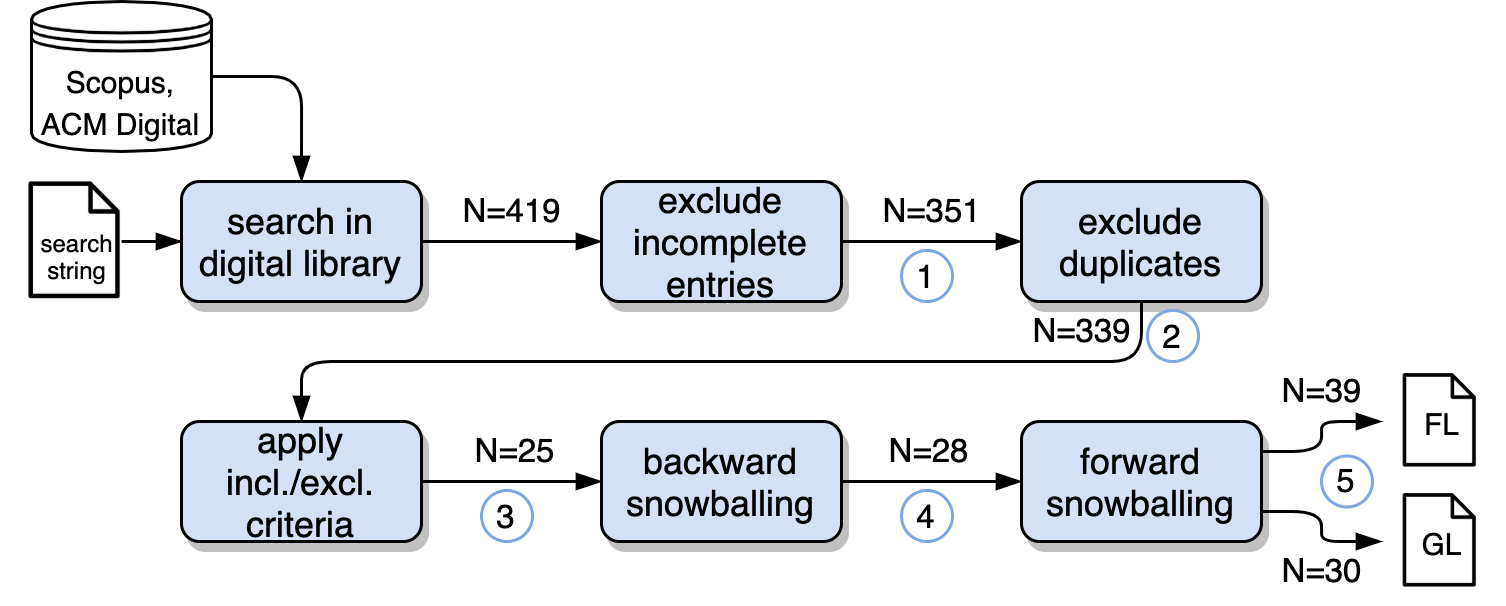
\includegraphics[width = 0.7\textwidth]{images/search-process.png}
 \caption{Literature search process workflow. In every step we denote the number of publications by $N=x$. The numbers 1 to 6 correspond to the CSV-files which contain all the retrieved literature in the particular step.}
 \label{fig:search-process}
\end{figure}

In preparation for this master thesis, we performed an extensive literature search and documented every step to make it reproducible. \cref{fig:search-process} shows the workflow of our literature search process. The complete documentation of the search process including the search strings and results with the retrieved literature will be made available in the GitHub project \url{https://github.com/mathebell/model-watermarking}.

We distinguish between the following types of publications: \textit{formal literature} (FL), i.e. peer-reviewed literature such as book sections, conference papers, journal articles, and \textit{grey literature} (GL), i.e. literature that did not undergo a peer-review process, such as pre-prints (published on repositories such as arXiv, or university repositories, author's websites, etc.) However, in its definition, grey literature does not only consist of pre-prints but can also be formed by blogs, interviews, wikis and many more document types \cite{mahood_searching_2014}, \cite{noauthor_greynet_nodate}. In this thesis, as the subject of watermarking of ML models has not produced such types of GL yet, it does however only consist of pre-prints.

\begin{figure} 
 \centering
 \begin{subfigure}[b]{0.48\linewidth}
 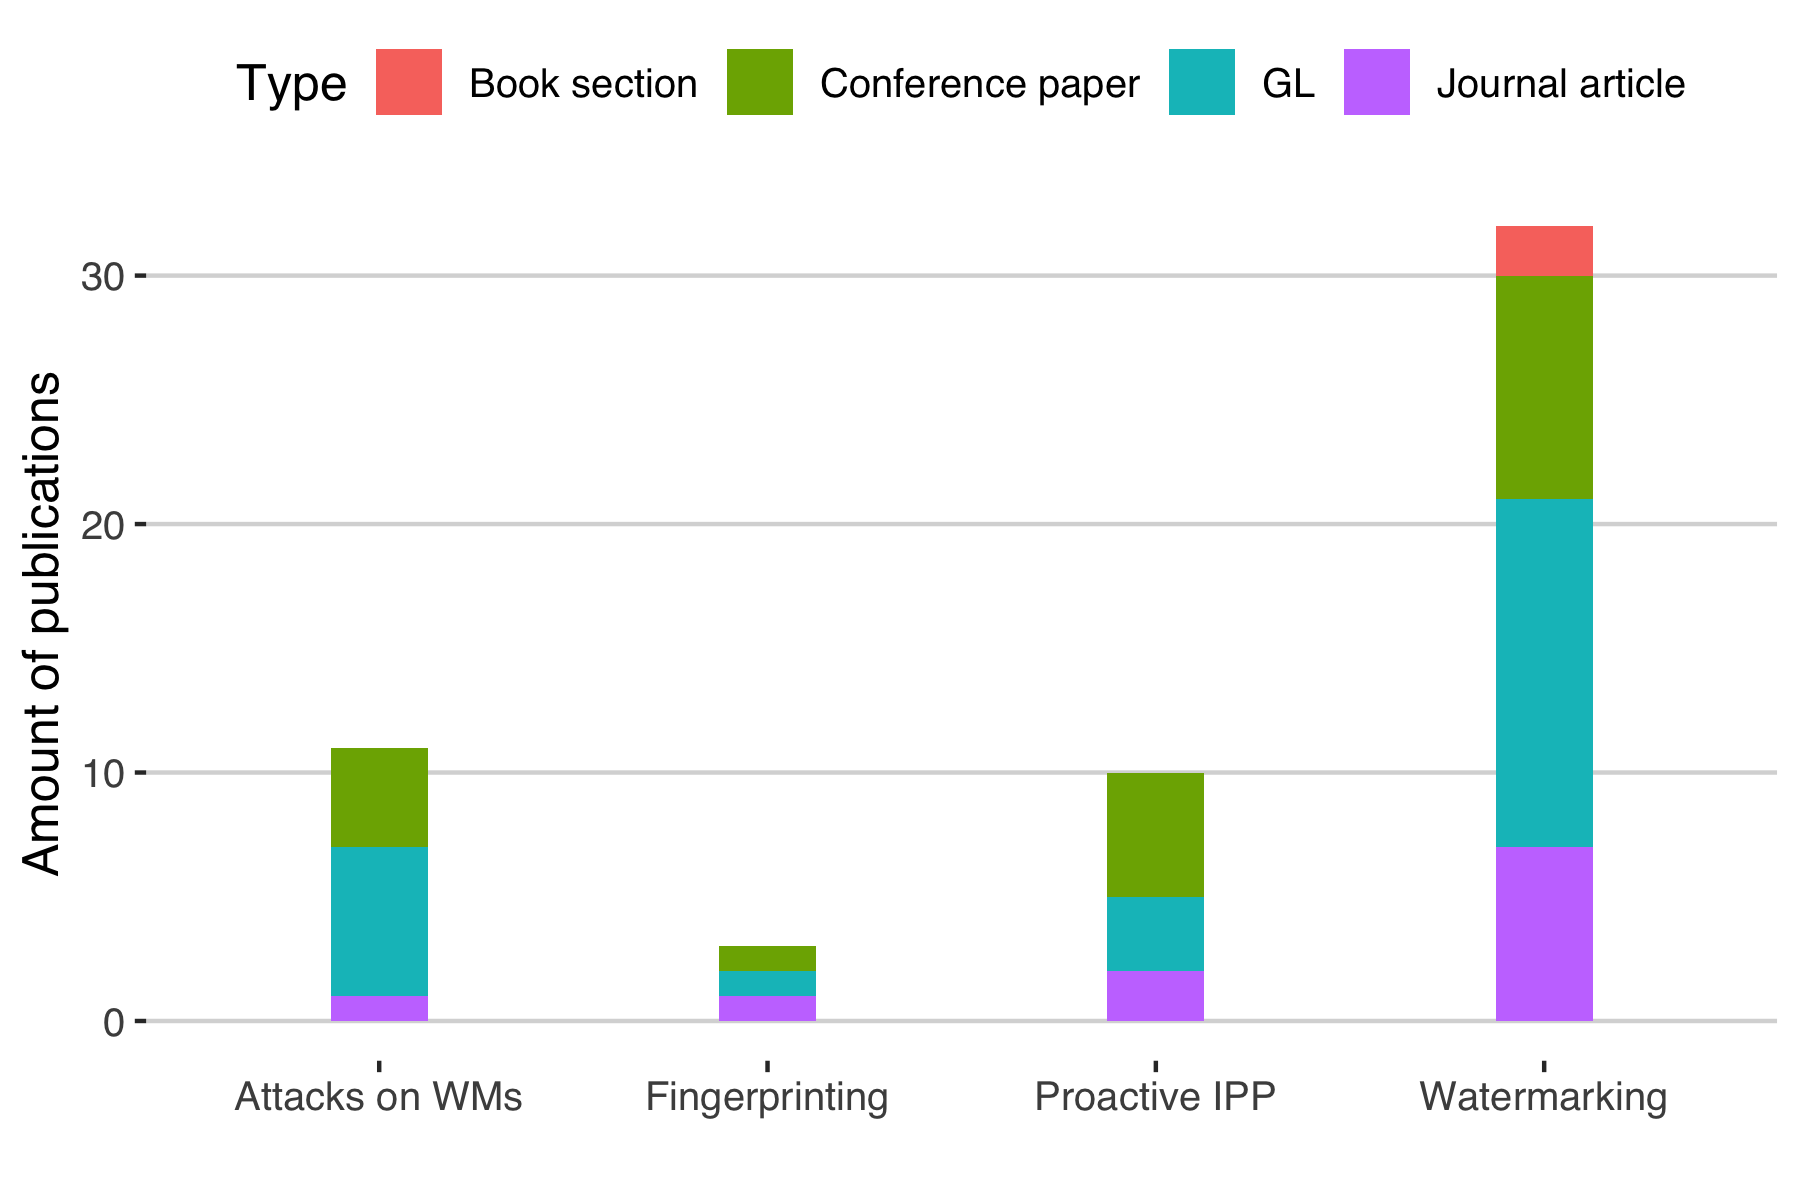
\includegraphics[width =\linewidth]{images/literature_types.png}
 \caption{Across different topics regarding ML IPP}
 \label{fig:aufteilung}
 \end{subfigure}
 \hfill
 \begin{subfigure}[b]{0.48\linewidth}
 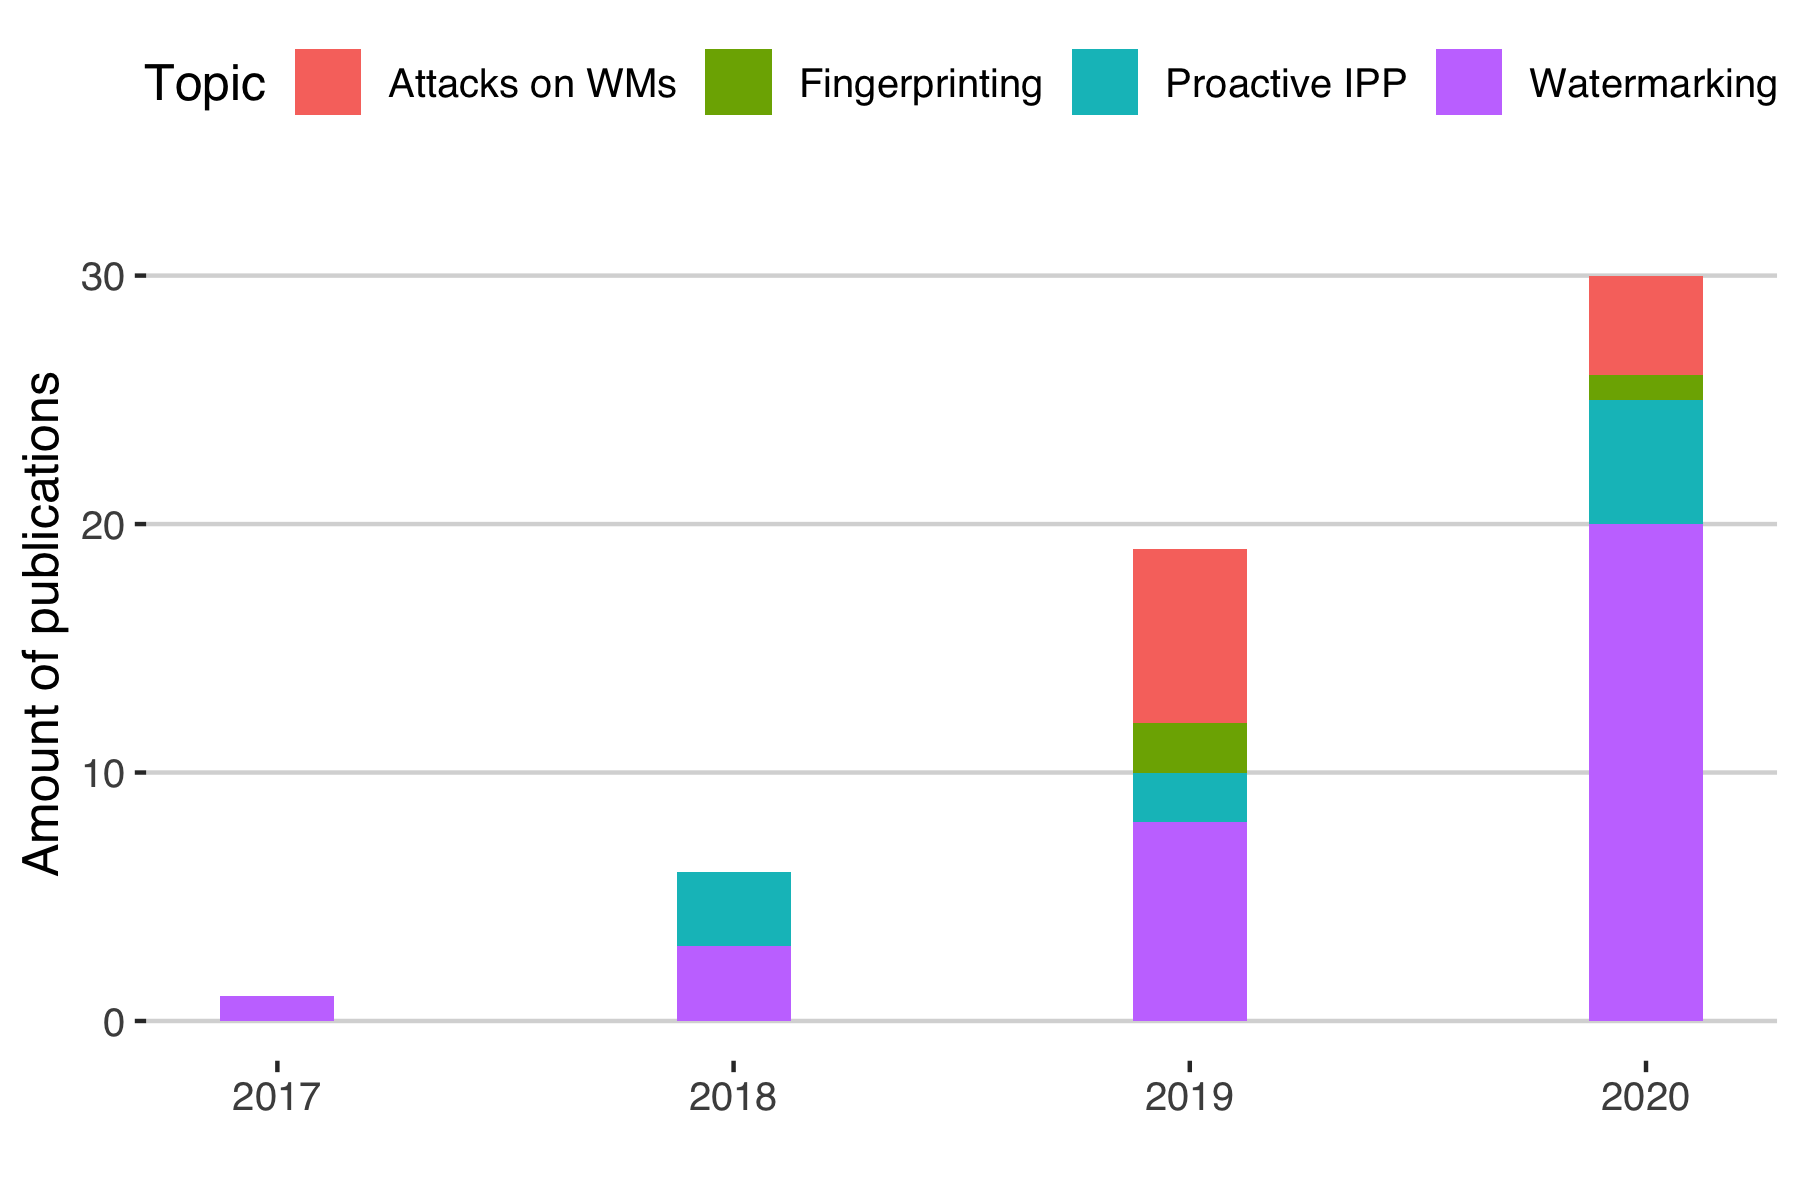
\includegraphics[width = \linewidth]{images/literature_years.png}
 \caption{Across the years for different topics}
 \label{fig:aufteilung-jahre}
 \end{subfigure}
 \caption{Literature distribution}
 \end{figure}

\cref{fig:aufteilung} shows the distribution of publications across the different topics in the various literature types. \textit{Attacks on WMs} include papers that propose attacks specifically crafted to disable a watermarking method or render it useless. \textit{Fingerprinting} and \textit{Watermarking} includes papers proposing a fingerprinting or watermarking method for ML models. \textit{Proactive IPP} includes papers on unrobust models and model access methods (cf. \cref{fig:overview}); these are not in the focus and are not discussed in more detail in this thesis. We can see that most papers were published regarding watermarking; however, there is also a significant number of papers on attacks published. Note, that some publications include both a novel attack to a scheme and a novel watermarking scheme, which is immune to this attack. Also, not all publications covering attacks are classified as such, as there is often a specific attack to a scheme, and a novel scheme immune to this attack, proposed in the same publication.

\cref{fig:aufteilung-jahre}, on the other hand, shows the distribution of publications across the publishing years. We see a rise in interest for this topic, with papers on attacks being mostly published in the last two years only.

\subsection{Inclusion/exclusion criteria} \label{appendix:method:criteria}

In order to provide reproducible documentation of the literature research, we defined the following inclusion and exclusion criteria to find the most relevant literature for the topic of IPP of ML models. Our inclusion criteria are:
\begin{itemize}
    \item Literature which proposes an IPP scheme for ML models
    \item Literature which proposes an attack on an IPP scheme for ML models
    \item Literature which evaluates or compares earlier schemes
\end{itemize}

Our exclusion criteria are:
\begin{itemize}
    \item (Near) Duplicates \footnote{If the titles are different but the content is very similar, we include all versions of the literature and note that. Later on, we will cite only the most complete version as suggested by Kitchenham et al. \cite{kitchenham_guidelines_2007}.}
    \item Literature which only \textit{uses} ML for multimedia watermarking, such as image watermarking
    \item Literature that only \textit{applies} previously published IP protection schemes, without a novel or large-scale evaluation
\end{itemize}

\section{Empirical evaluation}

As a first step we formulate research questions and define a study setting in \cref{ch:study_setting}, which includes benchmark architectures and datasets. We choose watermarking methods according to our defined selection criteria (cf. \cref{ch:study_setting}) and implement them in \cref{sec:implementation}. Afterwards, we analyse them based on experiments in \cref{sec:evaluation}. We synthesise our findings, answer the research questions and formulate selection guidelines in \cref{ch:conclusions}.

%1. research questions
%2. define study setting by choosing benchmark architectures and datasets
%3. choose wm methods
%4. implement wm methods
%5. run experiments
%6. synthesize finding -> answer research questions

%For the empirical evaluation of the chosen backdoor-based watermarking methods, we, first, define the study setting depending on the previously found key parameters. in order to find answers to our research questions. The research questions and the study setting are discussed in \cref{ch:study_setting}. Afterwards, we are going to implement the watermarking methods in a common framework, and evaluate and compare the methods regarding three main requirements for model watermarking in \cref{ch:empirical_comparison}.
%TODO: in general, this chapter could need a few more references to concepts / statements; I marked a few bit down the text, but there are other occasions where it fits

\chapter{Background}
\label{ch:background}

This chapter aims to equip the reader with the necessary background for the rest of the work. The definitions are formulated in a mathematical way. We expect the reader to be familiar with the notation.

\section{Machine Learning}
\label{sec:machinelearning}

\textit{Machine Learning} (ML) is a subfield of Artificial Intelligence (AI) and was defined by Tom Mitchell as "the study of computer algorithms that allow computer programs to automatically improve through experience" \cite{mitchell_machine_1997}.

The main objective in ML is the problem $\mathcal{P}$, i.e. the task that the ML model is trained to solve. %Such a problem $\mathcal{P}$ could be, e.g., classifying handwritten digits (image classification), grouping people based on different properties in order to identify outliers (clustering, anomaly detection) or solving a maze.
Common problems in ML are \cite{mohri_foundations_2018}:
% mehr oder weniger kopiert aus \cite{mohri_foundations_2018}
\begin{itemize}
    \item \textit{Classification}: "this is the problem of assigning a category to each example. For example, document classification consists of assigning a category such as politics, business, sports, or weather to each document, while image classification consists of assigning to each image a category such as car, train, or plane. The number of categories in such tasks is often less than a few hundred, but it can be much larger in some difficult tasks such as in text classification or speech recognition."
    % todo some math behind classification?
    \item \textit{Regression}: "this is the problem of predicting a real value for each item. Examples of regression include prediction of stock values or that of variations of economic variables. In regression, the penalty for an incorrect prediction depends on the magnitude of the difference between the true and predicted values, in contrast with the classification problem, where there is typically no notion of similarity between various categories."
    \item \textit{Clustering}: "this is the problem of partitioning a set of items into homogeneous subsets. Clustering is often used to analyse very large data sets. For example, in the context of social network analysis, clustering algorithms attempt to identify natural communities within large groups of people."
    %\item \textit{Dimensionality reduction}: this problem consists of transforming an initial representation of items into a lower-dimensional representation while preserving some properties of the initial representation. A common example is the Principal Component Analysis (PCA).
\end{itemize}

These problems are usually assigned to one of the three main categories in ML (cf. \cref{fig:machine_learning_structure}):

\begin{enumerate}
    \item \textbf{Supervised Learning} -- the model learns to make predictions based on a set of labelled data, e.g. classification or regression.
    \item \textbf{Unsupervised Learning} -- the model learns to find patterns in an unlabelled dataset, e.g. clustering or dimensionality reduction.
    \item \textbf{Reinforcement Learning} -- the model learns to master a task based on a feedback loop, e.g. playing a game.
\end{enumerate}

\begin{figure} %[H]
    \centering
    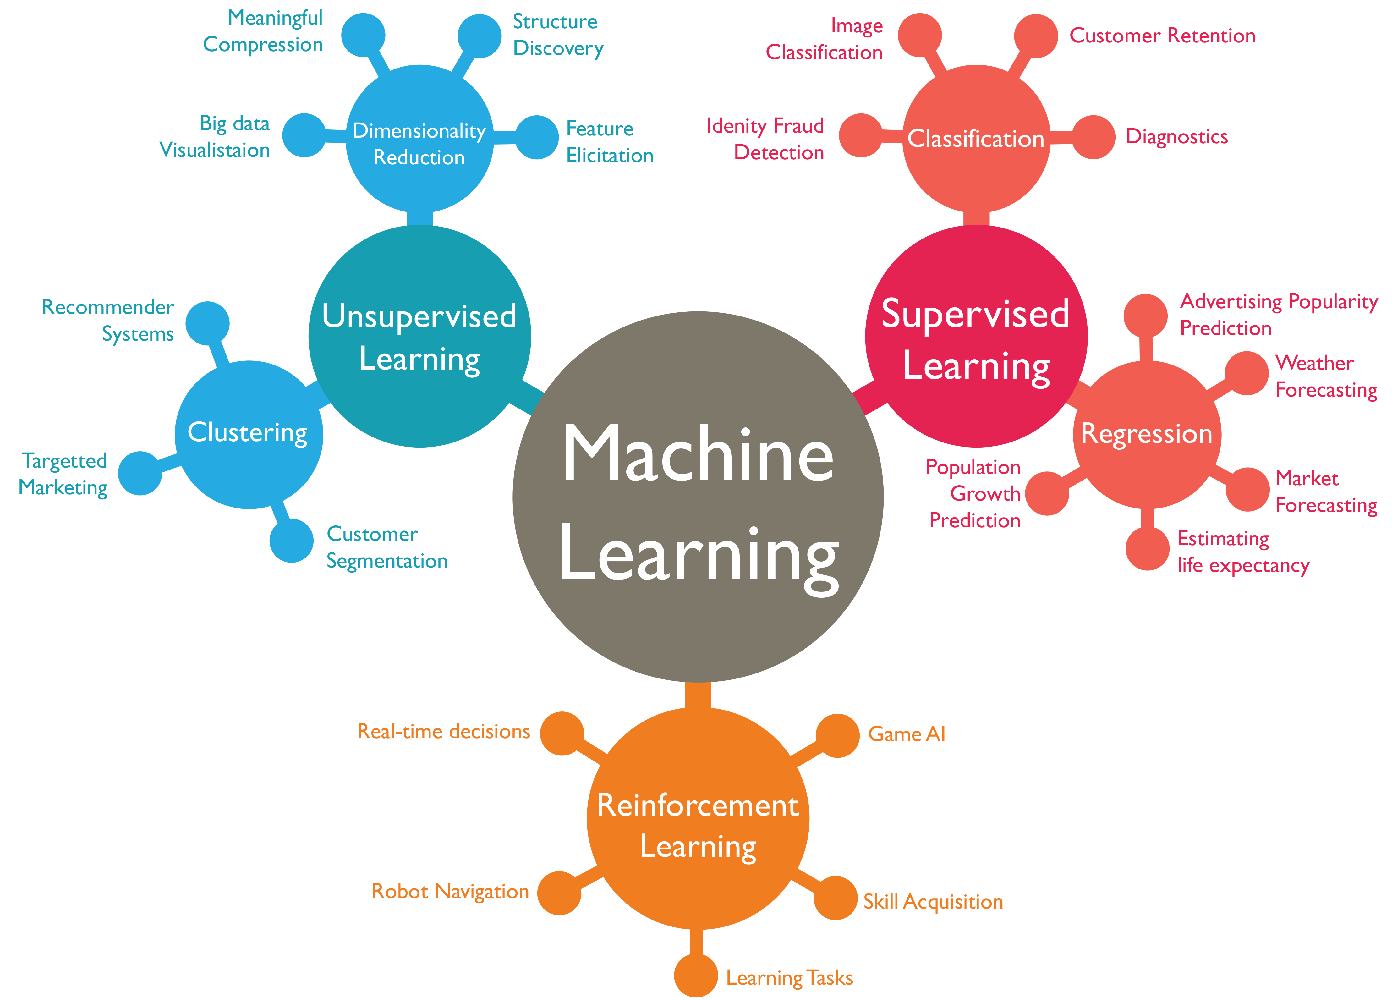
\includegraphics[width=.75\linewidth]{images/machine-learning.png}
    \caption{Three main categories of ML, their algorithms and use cases. Source: \cite{shewan_10_nodate}}
    \label{fig:machine_learning_structure}
\end{figure}

%Current research on Model Watermarking and therefore the thesis focuses on image classification. Image classification or image recognition is the most common application for Supervised Learning. Before we will dive into image classification and neural networks, w
We define typical terminology for Machine Learning \cite{mohri_foundations_2018}:
% mehr oder weniger kopiert aus \cite{mohri_foundations_2018}
\begin{itemize}
    \item \textit{Examples}: "Items or instances of data used for learning or testing. In image classification, these examples are images which we will use for learning and testing."
    \item \textit{Labels}: "Values or categories assigned to examples. In image classification, examples are assigned specific categories, for instance, car, train or plane."
    \item \textit{Parameters:} are values that control the behaviour of an ML model and are the instances that are updated during model training. We denote parameters, often also called \textit{weights}, by a vector $\mathbf{w}$, but also $\theta$ is a commonly used notation. 
    \item \textit{Hyperparameters}: "Free parameters that are not determined by the learning algorithm, but rather specified as inputs to the learning algorithm, such as the learning rate or the batch size."
    \item \textit{Training set}: "Examples or example-label pairs used to train a learning algorithm."
    \item \textit{Validation set}: "Examples or example-label pairs used to select appropriate values for the learning algorithm’s hyperparameters", or early stopping. Early stopping is a mechanism to stop training when the validation set performs best, in order to prevent from overfitting (cf. \cref{sec:overfitting}).
    \item \textit{Test set}: "Examples or example-label pairs used to evaluate the effectiveness of a learning algorithm. The test set is separate from the training and validation set and is not made available in the learning stage." The training, validation and test sets are pairwise disjoint subsets of the dataset. In Supervised Learning, the training, validation and test sets consist of example-label pairs, in unsupervised learning, on the other hand, only of examples.
    \item \textit{Loss function}: "A function, that measures the difference, or \textit{loss}, between a predicted label and a true label." We denote the loss function as $\mathcal{L}(\mathbf{w})$, where $\mathbf{w}$ is the ML model's parameter vector, since we usually want to minimise the loss function according to the model's parameters $\mathbf{w}$ (cf. \cref{eq:regression_loss}). However, in practice, the loss function is computed with the input of the true label and predicted label, and could therefore be denoted as $\mathcal{L}(y,\hat{y})$, where $y$ is the true and $\hat{y}$ the predicted label.
\end{itemize}

\subsection{Supervised Machine Learning}

In this work, we focus on Supervised Learning, especially image classification with Deep Learning (cf. \cref{sec:deep-learning}).
Let $\mathbf{X} \in \mathcal{D} \subset \mathbb{R}^n$, $n \geq 1$ be an input data point from a dataset $\mathcal{D}$ and $y$ the corresponding label, then we denote $f: \mathbb{R}^n \to \mathbb{R}$ as the function that maps the label to the example $f(\mathbf{X})=y$. We therefore train a supervised model $\mathcal{F}_{\mathbf{w}} : \mathbb{R}^n  \to \mathbb{R}$ to predict the data as well as possible, i.e. $\mathcal{F}_{\mathbf{w}}(\mathbf{X}) \approx f(\mathbf{X}), \; \forall \mathbf{X} \in \mathcal{D}$ with the trained parameter (weight) vector $\mathbf{w} \in \mathbb{R}^m$. The goal is to train the model in such a way that it predicts the right label also for unseen data, i.e. data that was not in the training set. %We define the model's \textit{accuracy}, or \textit{performance}, $\mathrm{Acc}(\mathcal{F}_{\mathbf{w}})$ and \textit{accuracy error} $\epsilon$ as
%\begin{align}
%  \mathrm{Acc}(\mathcal{F}_{\mathbf{w}}) = %\mathrm{Pr}(\mathcal{F}_{\mathbf{w}}(\mathbf{X}) = f(\mathbf{X})) %= 1 - \epsilon \quad \forall \mathbf{X} \in  \mathbb{R}^n,
%\end{align}
%where $\mathrm{Pr}(\cdot)$ denotes the probability of an event.

\begin{table} %[H]
    \centering
    \begin{tabular}{|c|c|c|}
    \hline
         & Predicted Yes & Predicted No \\
         \hline
       Actual Yes  &  {\color[HTML]{036400} True Positive (TP)} & {\color[HTML]{CB0000} False Negative (FN)} \\
       \hline
       Actual No & {\color[HTML]{CB0000} False Positive (FP)} & {\color[HTML]{036400} True Negative (TN)} \\ \hline
    \end{tabular}
    \caption{Confusion matrix of a two-class problem.}
    \label{tab:confusion_matrix}
\end{table}

In practice, the \textit{performance} of different models is compared via the model's \textit{accuracy} on the test set, the test accuracy, i.e. the fraction of total records that are correctly predicted by the model. The \textit{accuracy error} is then the difference between $100\%$ and the accuracy. In notation of the confusion matrix (cf. \cref{tab:confusion_matrix}) the accuracy on the dataset $\mathcal{D}$ is computed as
\begin{align}
    \mathrm{Accuracy}(\mathcal{F}_{\mathbf{w}}, \mathcal{D}) = \frac{TP+TN}{TP+TN+FP+FN}.
\end{align}

In the context of watermarking, we will use the terms false positive and false negative regularly, however, with a slightly different meaning. A watermarking method should have both a low false positive and a low false negative rate when triggering watermarks. We will explain the terms in \cref{sec:requirements}.

For classification problems with a large number of classes, the \textit{top N accuracy} is commonly used, since the model might not be able to predict the right class exactly, but the right class might be among the top $N$ predictions. The previously explained accuracy is then the top 1 accuracy as the prediction is only counted as TP or TN when it hits exactly the right class. For the top 3 accuracy, the prediction is counted as a TP or TN also when the true class is not the first, but among the first 3 predictions.

During model training, the model parameters are learned based on the training data. Some learning algorithms iteratively adapt their parameters, by minimising some kind of a loss function. Training accurate models often requires multiple training iterations, but not always as (simple cases of) linear regression can be solved non-iteratively as well.

There is a number of different ML models, e.g. \textit{Linear Regression}, \textit{Decision Tree} \cite{breiman_classification_2017}, \textit{k-Nearest Neighbor} (k-NN) \cite{altman_introduction_1992}, \textit{Perceptron} \cite{freund_large_1999}, etc. In the text below, we describe linear regression and perceptron in more detail.

\paragraph{Linear Regression} In a general formulation, linear regression finds the best fit line through the data, i.e. it finds the ideal parameter vector $\mathbf{w}=(w_0, w_1, \dots, w_{m-1})^\top \in \mathbb{R}^{m}$ (here $m=n+1$), so that for unknown data $\mathbf{X}=(x_1, x_2, \dots, x_n)^\top \in \mathbb{R}^n$ the real value is predicted by
\begin{align}
    \mathcal{F}_{\mathbf{w}}(\mathbf{X}) &= \sum_{i=1}^{n} w_i x_i + w_0 \\
    &= \mathbf{w}^\top \mathbf{X} + w_0,
\end{align}
where $w_0$ is the so-called \textit{bias} and often denoted as $b$.
This is done by minimising the mean squared error, which acts as loss function $\mathcal{L}$. Let the labelled training set $\mathcal{D} = \{(\mathbf{X}^1, y^1), (\mathbf{X}^2, y^2), \dots, (\mathbf{X}^k, y^k)\}$ be of size $k$, then the corresponding optimisation problem is
\begin{align} \label{eq:regression_loss}
    \min_{\mathbf{w} \in \mathbb{R}^m} \mathcal{L}(\mathbf{w}) = \min_{\mathbf{w} \in \mathbb{R}^m} \frac{1}{k} \sum_{j=1}^k \left(\mathbf{w}^\top \mathbf{X}^j + w_0 - y^j \right)^2.
\end{align}

\begin{figure}
    \centering
    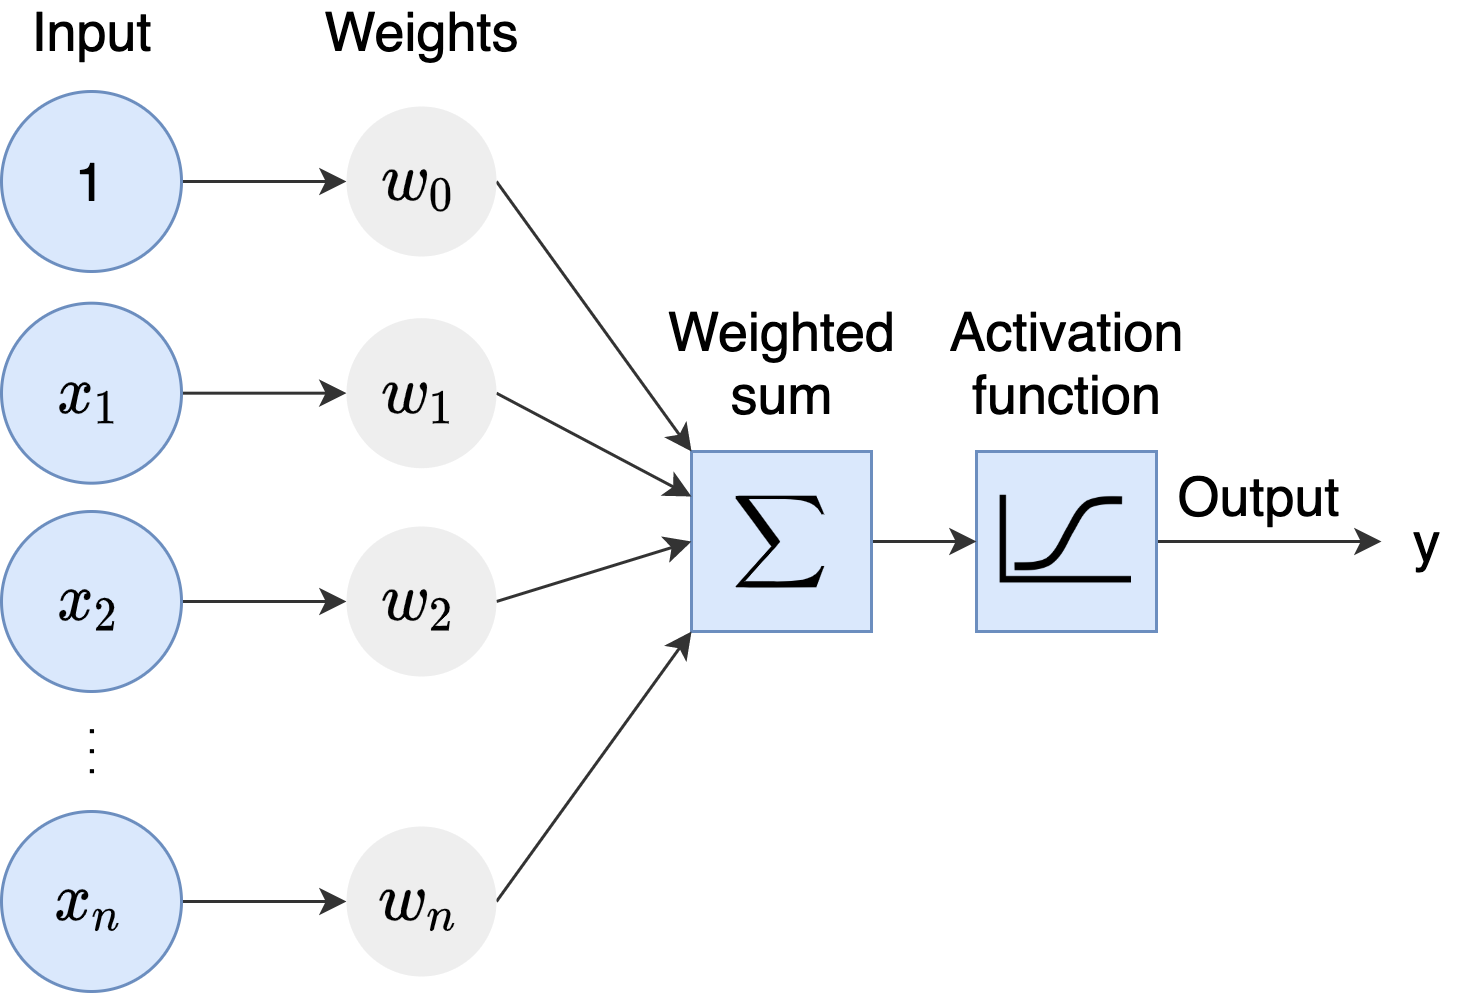
\includegraphics[width=0.7 \linewidth]{images/perceptron.png}
    \caption{A perceptron}
    \label{fig:perceptron}
\end{figure}

%All of the classifiers discussed below are categorised as \textit{Artificial Neural Networks} (ANNs), or just neural networks. An ANN, motivated by the human brain, is a collection of \textit{nodes}, or \textit{neurons}, which are connected through \textit{layers}. A layer consists of several nodes and, in its simplest form, a feed-forward layer, passes the information to (and only to) the next layer.

\paragraph{Perceptron} A \textit{perceptron} is a binary classifier and builds the basis for an \textit{Artificial Neural Network} (ANNs). An ANN, motivated by the human brain, is a collection of \textit{nodes}, or \textit{neurons}, which are connected through \textit{layers}. A layer consists of several nodes and, in its simplest form, a feed-forward layer, passes the information to (and only to) the next layer. 
Perceptron is the simplest form of ANN. It consists of only one neuron and outputs either $0$ or $1$. \cref{fig:perceptron} shows a perceptron that takes $n$-dimensional data as input. The output is computed by a linear combination of the input $\mathbf{X}=(x_1,x_2,\dots,x_n$) using the weights $\mathbf{w}=(w_0, \dots, w_n)$ 
\begin{align}
    \sum_{i=1}^n w_i x_i + w_0 = \mathbf{w}^\top \mathbf{X} + w_0
\end{align}
and applying a threshold step function with the threshold s
\begin{align}
    y = 
        \begin{cases}
        1 & \mathrm{for}\; \mathbf{w}^\top \mathbf{X} + w_0 \geq s\\
        0 & \mathrm{for}\;  \mathbf{w}^\top \mathbf{X} + w_0 < s
        \end{cases}.
\end{align}
During training, the weights of the perceptron are updated iteratively. Given a dataset consisting of example-label pairs $\mathcal{D} = \{(\mathbf{X}^1, y^1), (\mathbf{X}^2, y^2), \dots, (\mathbf{X}^k, y^k)\}$, we pass each example through the perceptron and update the weights according to the prediction. Let $\hat{y}^i$ be the predicted label for the input $\mathbf{X}^i$, then the weights are updated by
\begin{align*}
w_i^{\mathrm{new}} = w_i + \alpha (y^i - \hat{y}^i)x_i, \quad i=1, \dots n, 
\end{align*}
where $\alpha$ is the learning rate, which is an instance of the hyperparameters. This process is repeated until the prediction is correct for all examples in the dataset.
More complex types of ANNs are discussed in the following section.

% http://alexlenail.me/NN-SVG/LeNet.html
\subsubsection{Deep Learning} \label{sec:deep-learning}
\begin{figure} %[H]
    \centering
    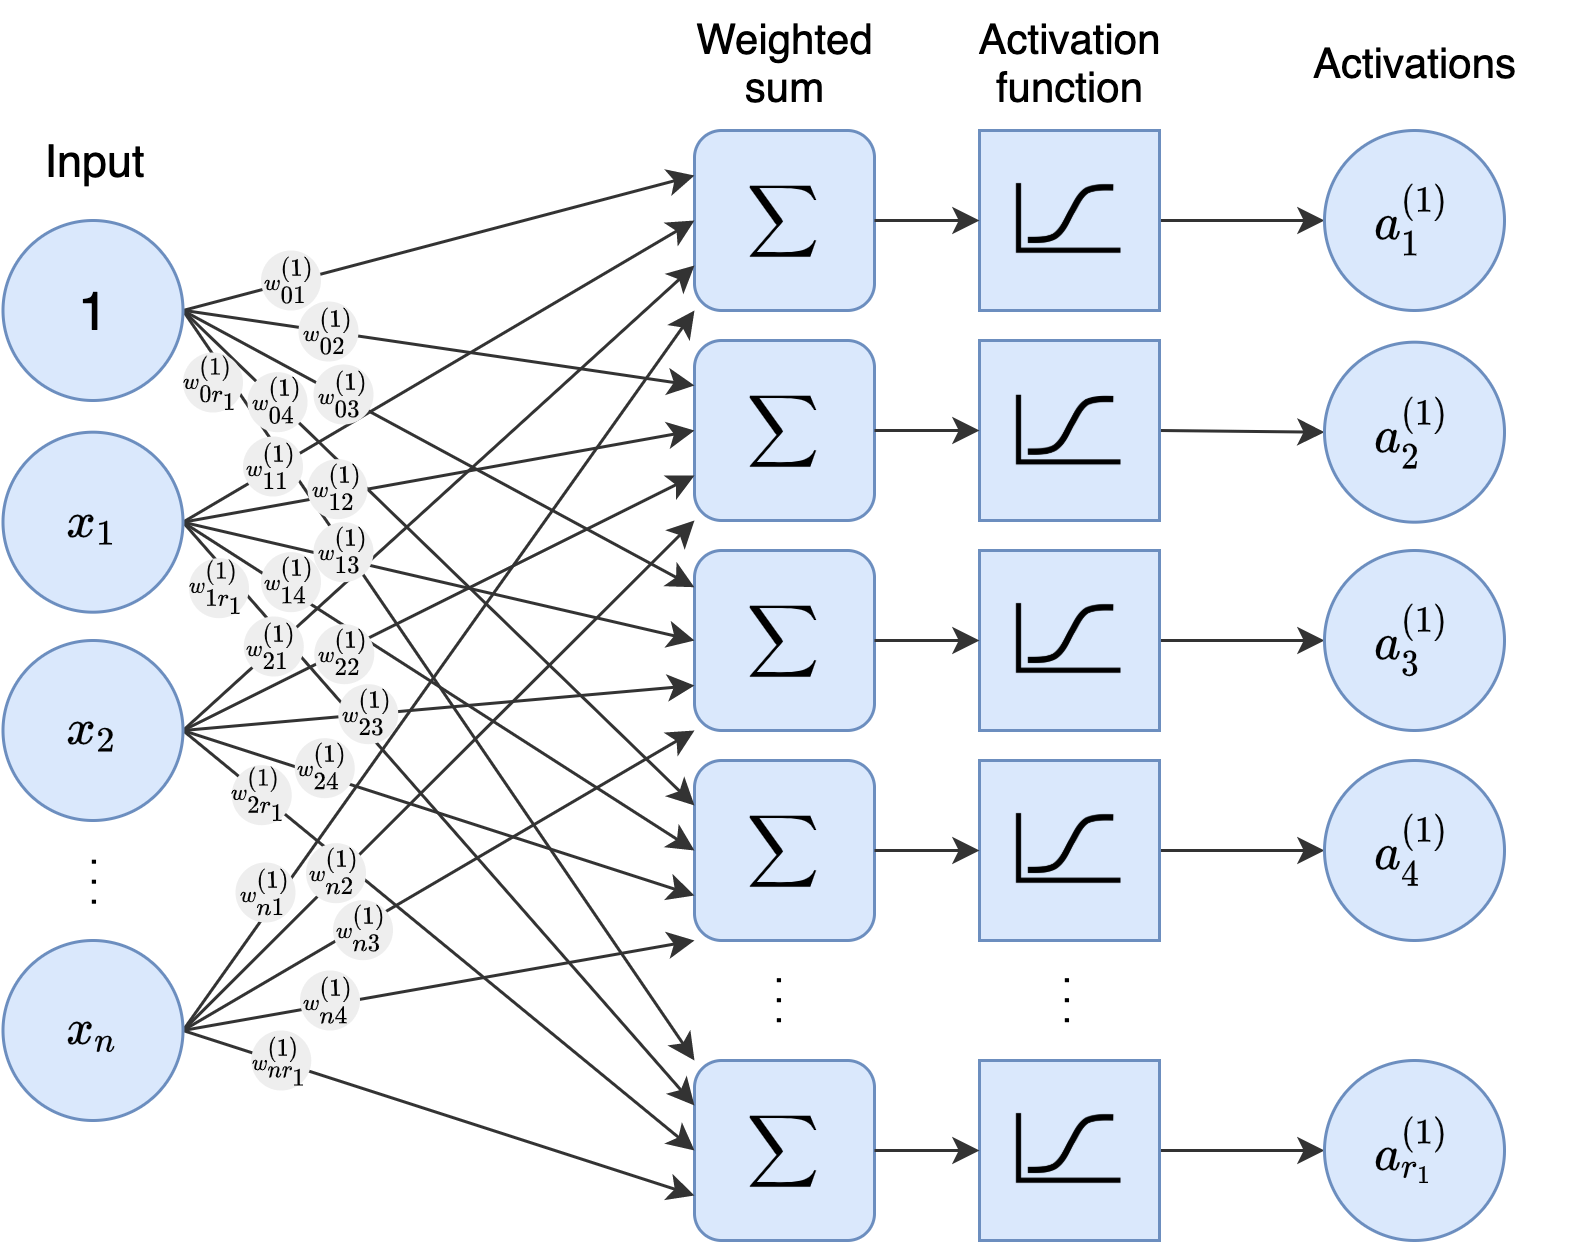
\includegraphics[width = 0.9\linewidth]{images/MLP.png}
    \caption{Computation of first layer in an MLP.}
    \label{fig:MLP}
\end{figure}

Deep Learning \cite{goodfellow_deep_2016} (DL) is a type of Machine Learning that achieves remarkable results on many tasks, by dividing a problem into many sub-problems. The basis for Deep Learning is a \textit{Multi-Layer Perceptron} (MLP). An MLP is a perceptron with at least one hidden layer. The hidden layer is again composed of perceptrons, as it is visualised in \cref{fig:MLP}. A feed-forward \textit{Deep Neural Network} (DNN) is an MLP with multiple (at least two) hidden layers. In general, the term DNN can be any ANN, not only MLP, with more than one hidden layer.
%The input layer is connected via hidden layers to the output layer which indicates the predicted label. \Cref{fig:neural_network} shows an illustration of a DNN.

We will now explain the computations in an MLP, but first we have to define the notation. We denote the model's parameters or weights with $\mathbf{w}$, but also $\theta$ is frequently used in other literature. As shown in \cref{fig:MLP}, we denote the input to a neural network as $\mathbf{X}= \left(x_1, x_2, \dots, x_n \right)^\top \in \mathbb{R}^n$, the weights connecting the input to the first node of the first hidden layer as $\mathbf{w}_1^{(1)} = \left(w_{11}^{(1)}, w_{21}^{(1)}, \dots, w_{n1}^{(1)} \right)^\top$, the weights connecting the input to the second node of the first hidden layer as $\mathbf{w}_2^{(1)} = \left(w_{12}^{(1)}, w_{22}^{(1)}, \dots, w_{n2}^{(1)} \right)^\top$, etc. Let $n$ be the size of the input and $r_1$ the size of the first hidden layer, then the weights for the first hidden layer can be combined into a matrix (and also analogously for all the other layers):
\begin{align}
\mathbf{W}^{(1)} = \left(\mathbf{w}_1^{(1)}, \dots ,\mathbf{w}_{r_1}^{(1)} \right) = \left(
\begin{array}{ccc} 
w_{11}^{(1)} & \cdots & w_{1r_1}^{(1)} \\ 
\vdots & \ddots & \vdots \\ 
w_{n1}^{(1)} & \cdots & w_{nr_1}^{(1)} \\ 
\end{array}
\right)
\end{align}

The first hidden layer's activations are denoted as $\mathbf{a}^{(1)} = \left(a_1^{(1)}, a_2^{(1)}, \dots, a_{r_1}^{(1)}\right)^\top$, the second hidden layer's nodes as $\mathbf{a}^{(2)} = \left(a_1^{(2)}, a_2^{(2)}, \dots, a_{r_2}^{(2)}\right)^\top$. The weights connecting $\mathbf{a}^{(1)}$ to $\mathbf{a}^{(2)}$ are denoted as $\mathbf{W}^{(2)}$. And finally, if the neural network consists of $L$ hidden layers, then the last hidden layer $\mathbf{a}^{(L)}$ is connected to the output layer $\mathbf{a}^{(O)}$ through $\mathbf{W}^{(L)}$. Let the size of the $l$-th layer be $r_l$.

With $g$ being the activation function, the first hidden layer's nodes are then computed as
\begin{align} 
    a_1^{(1)} &= g\left(\sum_{i=1}^{n} w_{i1}^{(1)} x_i + w_{01}^{(1)} \right) = g\left( {\mathbf{w}_1^{(1)}}^\top \mathbf{X} + w_{01}^{(1)} \right), \label{eq:first_layer_comp_1} \\
    &\vdots \nonumber \\
    a_{r_1}^{(1)} &= g\left(\sum_{i=1}^{n} w_{ir_1}^{(1)} x_i + w_{0r_1}^{(1)} \right) = g\left( {\mathbf{w}_{r_1}^{(1)}}^\top \mathbf{X} + w_{0r_1}^{(1)} \right), \label{eq:first_layer_comp_r1}
\end{align}
and directly fed into the computation for the second hidden layer:
\begin{align}
    a_1^{(2)} &= g\left(\sum_{j=1}^{r_1} w_{j1}^{(2)} a_j^{(1)} + w_{01}^{(2)} \right) = g\left(\sum_{j=1}^{r_1} w_{j1}^{(2)} g\left(\sum_{i=1}^{n} w_{ij}^{(1)} x_i + w_{0j}^{(1)} \right) + w_{01}^{(2)} \right), \label{eq:second_layer_comp_1} \\
    &\vdots \nonumber \\
    a_{r_2}^{(2)} &= g\left(\sum_{j=1}^{r_1} w_{jr_2}^{(2)} a_j^{(1)} + w_{0r_2}^{(2)} \right) = g\left(\sum_{j=1}^{r_1} w_{jr_2}^{(2)} g\left(\sum_{i=1}^{n} w_{ij}^{(1)} x_i + w_{0j}^{(1)} \right) + w_{0r_2}^{(2)} \right). \label{eq:second_layer_comp_r2}
\end{align}
Iteratively, we obtain the formula for the $l$-th node in the output layer:
\begin{align}
a_l^{(O)} &= g\left(\sum_{m=l}^{r_{L}} w_{ml}^{(O)} a_m^{(L)} + w_{0l}^{(O)} \right) \label{eq:last_layer_comp_1} \\
&= g\left(\sum_{m=l}^{r_L} w_{ml}^{(O)} \cdots g\left(\sum_{j=1}^{r_1} w_{jk}^{(2)} g\left(\sum_{i=1}^{n} w_{ij}^{(1)} x_i + w_{0j}^{(1)} \right) + w_{0k}^{(2)} \right) \cdots + w_{0l}^{(O)} \right) \label{eq:last_layer_comp_2}
\end{align}

The activation function $g$ decides, depending on the weighted sum, if a node should be activated or not, i.e. if the output of the node will be used for further computations or not. Common activation functions are the \textit{Heaviside step function}
\begin{align}
    g(x) = 
        \begin{cases}
        1 & \mathrm{for}\;  x \geq 0 \\
        0 & \mathrm{for}\; x < 0
        \end{cases},
\end{align}
a piecewise linear function, e.g., 
\begin{align}
    g(x) = 
        \begin{cases}
        1 & \mathrm{for}\; x \geq \frac{1}{2} \\
        x + \frac{1}{2} & \mathrm{for}\;  -\frac{1}{2} < x < \frac{1}{2} \\
        0 & \mathrm{for}\; x \leq -\frac{1}{2}
        \end{cases},
\end{align}
the \textit{sigmoid function} (which is used as a symbolic example in \cref{fig:MLP})
\begin{align}
    g(x) = \frac{1}{1+e^{-t}},
\end{align}
or, also a piecewise linear function, the \textit{Rectified Linear Unit} (ReLU) activation function
\begin{align}
    g(x) = \mathrm{max}(0,x).
\end{align}
The latter one is commonly used in Deep Learning, as only the neurons with a positive value are activated and therefore not all of them get activated at once as they would with a sigmoid function, being far more computationally efficient. There exist many other variations of ReLU, e.g. \textit{leaky ReLU} \cite{maas_rectifier_2013} and \textit{parameterised ReLU} (PReLU) \cite{he_delving_2015}, just to name a few. Leaky ReLU activates neurons also with a negative value, but weights it small:
\begin{align}
    g(x) = 
        \begin{cases}
        x & \mathrm{for}\;  x > 0 \\
        0.01x & \mathrm{for}\; x \leq 0
        \end{cases}
\end{align}
The PReLU takes the idea further and introduces a parameter which is learned during training:
\begin{align}
    g(x) = 
        \begin{cases}
        x & \mathrm{for}\;  x > 0 \\
        ax & \mathrm{for}\; x \leq 0,
        \end{cases}
\end{align}
with $a$ being the additional.

In order to solve the classification problem, we need a loss function that will be minimised during model training.
%Compared to the loss function in \cref{eq:regression_loss}, we cannot measure a "distance" between the predicted value and the true value by computing the mean squared error. Therefore, t
The function that is commonly used in classification is the \textit{Categorical Cross Entropy loss} function. It is used whenever an output vector is returned instead of one label. First, the \textit{Softmax} function $S$ is applied to the output vector to get output probabilities, i.e. values between 0 and 1, with the highest value corresponding to the model's prediction:
\begin{align}
    S\left(a^{(O)}_i\right) = \frac{\exp a^{(O)}_i}{\sum_j \exp a^{(O)}_j}
\end{align}
Given the input $\mathbf{X}$, a one-hot encoded label vector $\mathbf{y}=(y_1,y_2, \cdots, y_C) \in \{0,1\}^C$, where $C$ is the number of classes in the model, and the output vector of the model $\mathcal{F}_{\mathbf{W}}(\mathbf{X})=\mathbf{a}^{(O)}(\mathbf{X})$, the categorical cross entropy loss is then computed by
\begin{align}
    \mathcal{L}(\mathcal{F}_{\mathbf{W}}(\mathbf{X}), \mathbf{y}) &= - \sum_{i}^C y_i \log \left( \frac{\exp a^{(O)}_i(\mathbf{X})}{\sum_j \exp a^{(O)}_j(\mathbf{X})} \right) \\
    &= - \log \left( \frac{\exp a^{(O)}_p(\mathbf{X})}{\sum_j \exp a^{(O)}_j(\mathbf{X})} \right) \\
    &= - \log \left( S\left(a^{(O)}_p\right) \right),
\end{align}
with $p$ being the position in the output vector corresponding to the true label. The second equation holds since the label vector is one-hot encoded and all of the other terms are cancelled out. Therefore, the cross entropy loss returns high values for a small value in the output probabilities vector and vice versa, working as a penalty function. A perfect prediction with a one-hot encoded output probabilities vector would results in a loss of zero, which the model aims to learn during training. 

Since the output vector $\mathbf{a}^{(O)}$ mainly depends on the weights $\mathbf{W} = (\mathbf{W}^{(1)}, \mathbf{W}^{(2)}, \dots, \mathbf{W}^{(L)})$ of the DNN, we can formulate the optimisation problem for the DNN as
\begin{align}
    \min_{\mathbf{W} \in \mathbb{R}^{m}} \mathcal{L}(\mathbf{W},\mathcal{F}_{\mathbf{W}}(\mathbf{X}), \mathbf{y}) = \max_{\mathbf{W} \in \mathbb{R}^{m}} \log \left( \frac{\exp a^{(O)}_p}{\sum_j  \exp a^{(O)}_j} \right),
\end{align}
where here $\mathbf{W} \in \mathbb{R}^m$ denotes the flattened version of the matrix $\mathbf{W}$ with length $m = nr_1 + \sum_{i=2}^L r_{i-1}r_i$.

In order to solve this optimisation problem, a multitude of optimisation algorithms has been introduced \cite{goodfellow_deep_2016}. \textit{Gradient descent} is the most basic gradient-based optimisation algorithm and forms the basis for the more advanced ones. The algorithm updates the parameters after computing the gradients based on the whole training set and is therefore not recommended to use with large datasets. Let $\mathcal{D} = \{(\mathbf{X}^1, y^1), (\mathbf{X}^2, y^2), \dots, (\mathbf{X}^k, y^k)\}$ the training set, then the update rule for the parameters is as follows
\begin{align}
    \mathbf{W}^{\mathrm{new}} = \mathbf{W} + \alpha \nabla_{\mathbf{w}} \sum_{i=1}^k \mathcal{L}(\mathbf{W},\mathcal{F}_{\mathbf{W}}(\mathbf{X}^i), y^i),
\end{align}
where $\alpha$ denotes the learning rate. The algorithm converges even with a fixed learning rate, provided that the gradients of the loss function are Lipschitz continuous.

A more commonly used algorithm is the \textit{Stochastic Gradient Descent} (SGD), which estimates the gradients based on a batch of training samples. Given a batch of $m$ training samples $\{(\mathbf{X}^1, y^1), (\mathbf{X}^2, y^2), \dots, (\mathbf{X}^m, y^m)\}$, the gradient estimate is computed by
\begin{align}
    \hat{\mathbf{g}} = \frac{1}{m} \sum_{i=1}^m \mathcal{L}(\mathbf{W},\mathcal{F}_{\mathbf{W}}(\mathbf{X}^i), y^i)
\end{align}
and the parameters are updated after running through a batch by
\begin{align}
    \mathbf{W}^{\mathrm{new}} = \mathbf{W} - \alpha \hat{\mathbf{g}}.
\end{align}

Another widely used algorithm is the \textit{Adam} optimiser \cite{kingma_adam_2015}, which is an extension of the SGD. Adam is an adaptive gradient descent algorithm, i.e. it adapts the learning rate per parameter. Some models tend to perform better optimised with Adam than with SGD.

\textit{Learning rate schedulers} adapt the (global) learning rate during training, dependent on the number of iterations, according to a pre-defined schedule. Two commonly used learning rate schedulers are \texttt{MultiStepLR} and \texttt{CosineAnnealingLR}. \textit{MultiStepLR} reduces the learning rate every $n$ epochs by a rate of, e.g., 0.1. The learning rate gets smaller every $n$ epochs. \textit{CosineAnnealingLR}, however, has a schedule that decreases the learning rate but also increases, in an overall downward trend.

\textit{Convolutional Neural Networks} (CNNs) \cite{krizhevsky_imagenet_2017} are a special type of DNNs where the hidden layers consist of convolutional, pooling and feed-forward layers. CNNs achieved a breakthrough in image recognition. The convolutional filters are applied to the image and enhance special features in an image, e.g. edges, lines or different shapes, and make it therefore possible to learn how to distinguish between objects. A schematic view of this process is shown in \cref{fig:cnn_features}.

\begin{figure}
    \centering
    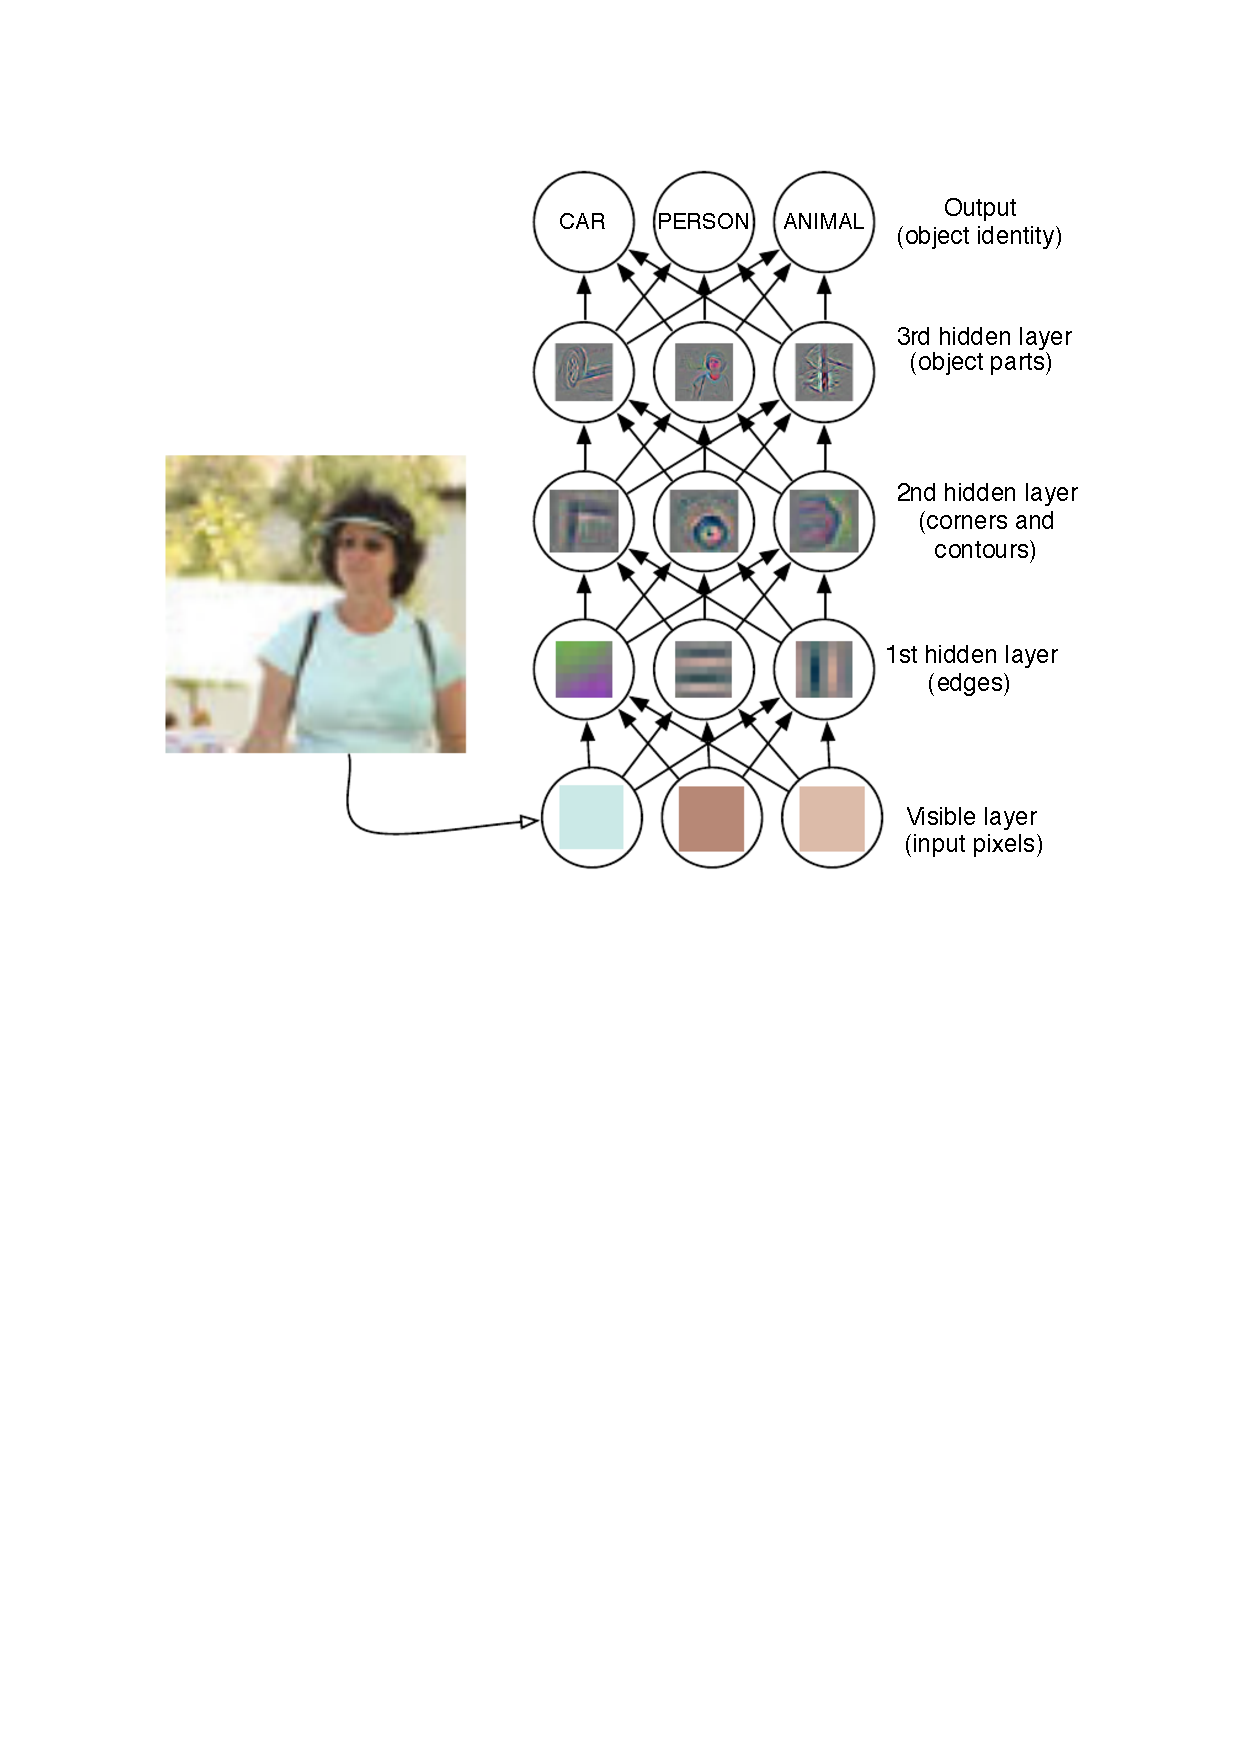
\includegraphics[width=0.7 \textwidth]{images/cnn_features.pdf}
    \caption{Convolutional filters in a Deep Neural Network enhancing features in an image. Usually, the first layers recognise simple features such as lines and corners by comparing the contrast of neighbouring pixels. With this information, the following layers are responsible for recognising whole object parts. In this manner, feeding the pixel information from the input through a series of layers consisting of convolutional, pooling and feed-forward layers, eventually results in a class prediction. Source: \cite{goodfellow_deep_2016}}
    \label{fig:cnn_features}
\end{figure}

Convolutional layers \cite{goodfellow_deep_2016} differ in computation compared to ordinary feed-forward layers as shown before in \cref{eq:first_layer_comp_1,,eq:first_layer_comp_r1,eq:second_layer_comp_1,eq:second_layer_comp_r2,eq:last_layer_comp_1,eq:last_layer_comp_2}. Convolutional layers consist of one of more convolutional \textit{filters} or \textit{kernels}. As the name already indicates, the layer performs a mathematical operation called convolution, which we would like to explain in detail. The following definitions are adapted from \cite{goodfellow_deep_2016}. The \textit{continuous mathematical convolution} is an operation on two functions of real arguments, say $f,g: \mathbb{R}^n \to \mathbb{C}$, and computed as
\begin{align}
    (f \ast g) (x) := \int_{\mathbb{R}^n} f(y) g(x-y)dy.
\end{align}
The mathematical convolution is a weighted mean value, for which every $f(y)$ is weighted by $g(x-y)$. If we deal with discrete functions, which for computational reasons is necessary, we define the \textit{discrete mathematical convolution} as
\begin{align}
    (f \ast g) [x] := \sum_{y=-\infty}^{\infty} f[y] g[x-y].
\end{align}
In Machine Learning, however, a \textit{convolution} performs a slightly different operation. Since we usually deal with multi-dimensional input data, e.g. images, of finite size, let the input $\mathbf{X} \in \mathbb{R}^{n \times n}$ and the kernel $\mathbf{K} \in \mathbb{R}^{m \times m}$ be two-dimensional and finite. Then, the convolution is computed as
\begin{align}
    (\mathbf{I} \ast \mathbf{K})[i,j] = \sum_m \sum_n \mathbf{I}[i+m,j+n] \mathbf{K}[m,n], \quad 1 \leq i,j \leq n-m+1
\end{align}
and the output is called \textit{feature map}. A schematic view of the computation is shown in \cref{fig:convolution}. Depending on the values of a kernel, the image is processed in a different way, in order to enhance the special features in an image. Those values of a kernel are iteratively updated during training, i.e. the model learns how to enhance features in order to distinguish between different objects. In this way, a CNN is able to classify images depending on special features in an image and therefore better at generalisation compared to image classification with an MLP.

%\red{TODO: show convolution filters for enhancement of horizontal/vertical lines}

Pooling layers \cite{goodfellow_deep_2016} serve as a summary of information after a convolutional layer. They reduce the dimension of data and help to make the representation become invariant to small changes in the input. Common pooling techniques are \textit{max} and \textit{average} pooling. Max pooling takes the maximum value within a rectangular neighbourhood and average pooling takes the average value.

%\red{TODO: Show 1-2 examples of current CNN architectures (do you show that later?)}


\begin{figure}
    \centering
    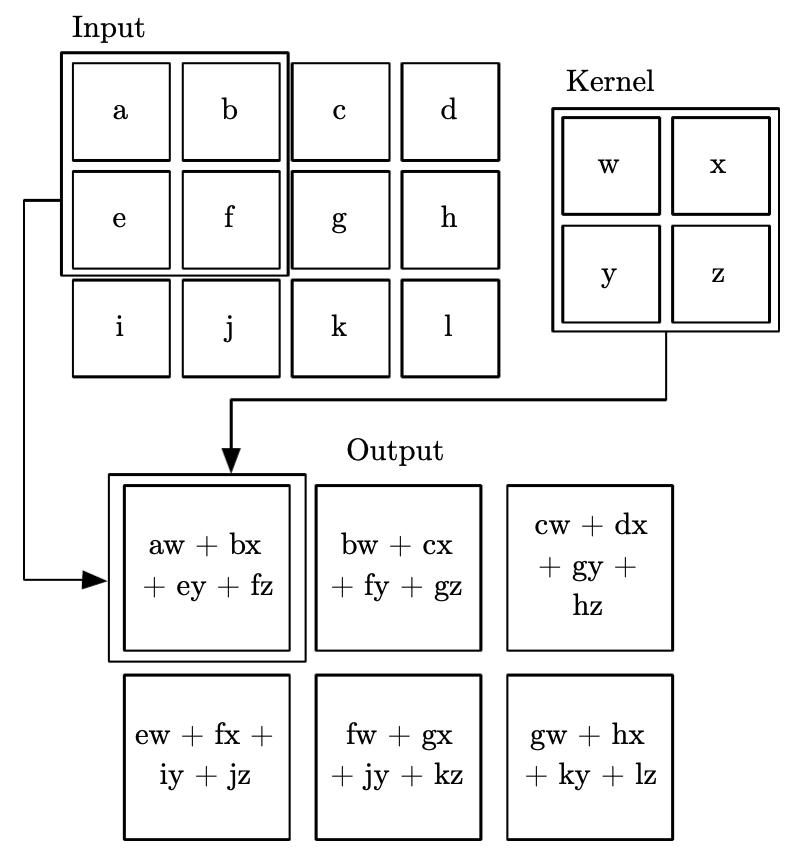
\includegraphics[width= 0.5 \textwidth]{images/convolution_deeplearning.png}
    \caption{Computation of convolutional filter with padding 1. Padding means how much the filter shifts on the input during the computation. With padding 2, e.g., the filter would move forward two values instead of one, in order to compute the next output value. Source: \cite{goodfellow_deep_2016}}
    \label{fig:convolution}
\end{figure}

\textit{Recurrent Neural Networks} \cite{rumelhart_learning_1986} (RNNs) are another special type of DNNs where the connections between neurons are not only limited to the neighbouring layer, like in feed-forward neural networks but can be connected to any other neuron and therefore forming a "memory" for the network. RNNs support sequential data and are especially important for non-static problems like speech recognition. Famous RNNs are the Long Short-Term Memory Network (LSTM) \cite{hochreiter_longshorttermmemory_1997} and Gated Recurrent Unit (GRU) \cite{cho_learning_2014}. \cref{fig:lstm_gru} shows an illustration for LSTM and GRU. LTSMs and GRUs have internal mechanisms called \textit{gates} that can regulate the flow of information. The gates are trained to distinguish which data in a sequence is important and which is not.

%source: https://towardsdatascience.com/illustrated-guide-to-lstms-and-gru-s-a-step-by-step-explanation-44e9eb85bf21
\begin{figure}
    \centering
    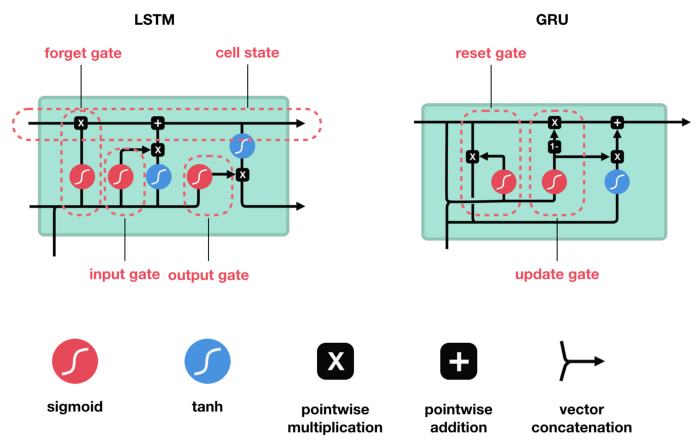
\includegraphics[width= 0.8 \linewidth]{images/LSTM_and_GRU.png}
    \caption{LSTM and GRU. Source: \cite{phi_illustrated_2018}}
    \label{fig:lstm_gru}
\end{figure}


%Common algorithms in Supervised Learning are \textit{Support Vector Machine} (SVM), \textit{Random Forest} and \textit{(Artificial) Neural Networks} (ANNs), especially \textit{Deep Neural Networks} (DNNs). A DNN is an feed-forward ANN with multiple fully-connected hidden layers. 


%https://towardsdatascience.com/https-medium-com-piotr-skalski92-deep-dive-into-deep-networks-math-17660bc376ba


%TODO: present examples of CNNs: LeNet \cite{lecun_gradient-based_1998}, AlexNet \cite{krizhevsky_imagenet_2017}, VGG \cite{simonyan_very_2014}, ResNet \cite{he_deep_2016} and DenseNet \cite{huang_densely_2017}, GoogLeNet
%TODO: examples RNN: Long Short-Term Memory Network (LSTM) \cite{hochreiter_long_1997} and Gated Recurrent Unit (GRU) \cite{cho_learning_2014}

%TODO: describe Graph Neural Networks, because it will be mentioned later. Daryna wrote: A \textit{Graph Neural Network} (GNN) is used to process the data represented in a graph structure \cite{scarselli_graph_2009}. The most famous application of such type of networks is Social Network Analysis (SNA). GNNs allows performing node classification, link prediction, or complete graph classification.


\subsubsection{Fine-Tuning}
% Fine-tuning with new data: Ross Girshick, Jeff Donahue, Trevor Darrell, and Jitendra Malik. 2014. Rich feature hierarchies for accurate object detection and semantic segmentation. In Proceedings of the IEEE conference on computer vision and pattern recognition. 580–587.
The process of \textit{Fine-Tuning} \cite{girshick_rich_2014}, training a model on different training data with a smaller learning rate, can be used for either improving the model or when using it for a slightly different purpose, in \textit{Transfer Learning} \cite{pan_survey_2010}. In this thesis, we use it either to embed a watermark or as a malicious modification to a well-trained model to remove unwanted information, e.g. a watermark.

\subsubsection{Overfitting} \label{sec:overfitting}
In training an ML model, \textit{overfitting} \cite{ying_overview_2019} is a common phenomenon. Overfitting means that the model is well-trained on the training data, but performs poorly on data that it has not seen before, e.g. the test set. Usually, this happens when the architecture is complex, but there is too little training data available. In this sense, the model has enough degrees of freedom so that it can "memorise" the training data rather than learn how to generalise.

One technique to prevent overfitting in ML models is \textit{regularisation} \cite{ying_overview_2019}. During model training, a \textit{parameter regulariser} is used. A regulariser is an additional term in a loss function, often in the form of a penalty term that controls the magnitude of the parameter values. The loss function $\mathcal{L}(\mathbf{w})$ with a regulariser is defined as
\begin{equation}
    \mathcal{L}(\mathbf{w}) = \mathcal{L}_0(\mathbf{w}) + \lambda \mathcal{L}_R(\mathbf{w}),
\end{equation}
where $\mathbf{w}$ is the parameter vector, $\mathcal{L}_0$ is the original loss function, $\mathcal{L}_R$ the regularisation term, and $\lambda$ an adjustable parameter. Several regularisers have been studied in the literature, e.g. the  $L_2$-regularisation, also called Ridge regularisation, or the $L_1$-regularisation, also called LASSO regularisation.

Another technique to prevent overfitting is \textit{early-stopping} \cite{ying_overview_2019}. During model training, the time when the model starts to overfit can be detected. It happens when the test or validation accuracy stops improving, but the train accuracy still does. With early-stopping, we stop the training when the validation loss is minimal. Since we only know that the validation loss is at its minimum when we train several iterations after we reached the minimum. An additional parameter for early-stopping is the \textit{patience}, the number of training iterations after the minimal validation loss was found, to confirm that this is indeed the right timing to stop training.

\subsubsection{Parameter Pruning}
Parameter pruning \cite{han_learning_2015} is a model compression technique, i.e. it is used to compress the model in order to reduce the storage and computation of the model. It has been shown that by applying parameter pruning, the number of parameters drops by a magnitude without any significant accuracy loss. The model parameters with the smallest absolute value are set to zero because one assumes that the weights with minimal values hold no or negligible information and can be cut out. In this thesis, we consider parameter pruning as either a targeted attack, as the attacker could assume that the pruned weights hold watermark information or as an accidental attack when the attacker wants to drop redundant parameters for storage reasons.

\subsection{Further ML techniques}
In the following, we introduce ML techniques that are mentioned in the thesis, but not as much of importance to the core work.

\textit{Federated Learning} \cite{yang_federated_2019} is an ML technique where multiple parties are involved in training the model on their data, without exchanging the data among each other, mostly for privacy-preserving goals.

\textit{Generative Adversarial Networks} (GANs) \cite{goodfellow_generative_2014} are an ML architecture that uses two DNNs to learn a task -- one DNN actually learns the task (the generator) and the other evaluates it (the discriminator). For instance, a common application area is picture generation. The generator learns to create pictures from scratch of, e.g. humans, and the discriminator evaluates its performance by comparing a set of real samples with the generated set. The discriminator has two possible outputs "real" and "fake". The goal of a GAN is that the discriminator outputs "real" for the images generated with the generator.

% todo: include img for GAN?

% autoencoder kommt vor in \cite{namba_robust_2019}
An \textit{autoencoder} is a special ANN that is commonly used for dimensionality reduction, that is to find a low-dimensional representation of high-dimensional data in an unsupervised manner. This is achieved by learning to copy its input to its output. It consists of an encoder and a decoder, and an internal (hidden) layer that describes a code learned to represent the input.

Knowledge \textit{Distillation} \cite{hinton_distilling_2015} is a type of compression technique that uses knowledge of a neural network (teacher network) to train a new smaller network (student network). A smaller model is computational less expensive and thus more appealing.

%Daryna wrote: Knowledge distillation~\cite{bucilua_model_2006,hinton_distilling_2015} is a model compression~\cite{cheng_survey_2017} method that allows to train a smaller network, using an already trained bigger network without decreasing accuracy. Usually, the bigger and smaller network are called teacher and student network, respectively. The main idea of this approach is that the student network is learning to duplicate the outputs of the teacher network on \textit{each} layer, not only the final output. This approach assumes white-box access to the teacher network, i.e. the architecture and model's weights \unsure{parameters is likely the better term} should be known.

\textit{Adversarial Examples} \cite{szegedy_intriguing_2014} are a kind of input that is created to fool a model. Usually, an original input (e.g. an image) is perturbed by some specially crafted noise such that the model is unable to classify the generated input correctly. The perturbation is kept minimal, to ideally not be noticeable by a human, or detection methods. Several methods to create Adversarial Examples have been proposed, the most well-known likely being the Fast Gradient Sign Method (FGSM) \cite{goodfellow_explaining_2015}.

\subsection{Model Extraction Attack}

A specific attack against the IP of ML models is the so-called \textit{Model Extraction Attack} (or Model Stealing Attack) \cite{tramer_stealing_2016}, which aims to reveal a model's internal characteristic or copy a complete model by only querying its API service. The target can be the architecture, parameters, decision boundary, functionality, or training hyper-parameters of the model.
% \cite{szyller_dawn_2020} has a nice section for model extraction.

\section{Watermarking} \label{sec:background:watermarking}
Digital watermarking is a well-studied procedure in e.g. multimedia Intellectual Property Protection (IPP) \cite{kahng_watermarking_1998} or relational databases \cite{kamran_comprehensive_2018}. The main idea is to embed a piece of signature in the data, e.g. image or audio, to deter malicious usage. This signature is often intended to be unnoticeable, however, perceptible watermarks are also commonly used in the multimedia domain; examples are logos or copyright notices that are added to images or videos to identify the author.
Non-perceptible watermarks, on the other hand, aim to avoid changing the perceptible impression of the data. This is also the type of watermark that we consider for the IPP of ML models. Digital watermarking is thus a form of steganography or information hiding, i.e. the practice of concealing a message within another message.
The hidden information must be embedded in such a way that no algorithm can remove or overwrite the watermark. Some recent digital watermarking techniques, e.g. for images, make use of DNNs in the embedding process \cite{zhong_automated_2020}; similarly, also attacks targeted to remove such watermarks are increasingly using deep learning techniques \cite{sharma_robust_2020}.

%Quiring et al. \cite{quiring_adversarial_2018}, for example, combines methods from model stealing to generate a \textit{substitute} model of a watermark detector, and then generates adversarial examples against this model, to obtain images with minimal perturbations that evade detection.

%Something like this should be somewere... but skipped for now
%Watermarking schemes for relational databases can as simplistic approach also be employed for white-box watermarking of ML models, as the parameters of these models can in most cases be represented as relational data.

In this thesis, we discuss (ML) model watermarking, i.e. the IP that has to be protected is an ML model. Model watermarking is related to multimedia or relational data watermarking, but the techniques differ since the protecting instance changed. 
Research on watermarking DNNs predominantly addresses image classification (cf. \cref{ch:sota}). The introduced terminology is thus strongly influenced by this application of ML, but we believe that the concepts are transferable to other input types as well.

At this point, we want to define the terminology that is common in model watermarking and is used throughout this work. A typical watermarking workflow is shown in \cref{fig:watermarking_workflow}. Watermark \textit{embedding} describes the process in which the watermark is placed into the model, e.g. via fine-tuning. We call watermark \textit{extraction} the process in which the embedded watermark is extracted from the model, but neither in a permanent (which is called \textit{watermark removal}) nor in a malicious way (which is called \textit{watermark detection}). Watermark extraction means that we want to identify if any, and which watermark is placed. 

Finally, during watermark \textit{verification}, the extracted watermark is compared to the model owner's watermark in order to prove ownership. Following certain rules (e.g. thresholding the watermark accuracy or (bit) error rate), it is then decided if the watermarks are the same.

\begin{figure}
    \centering
    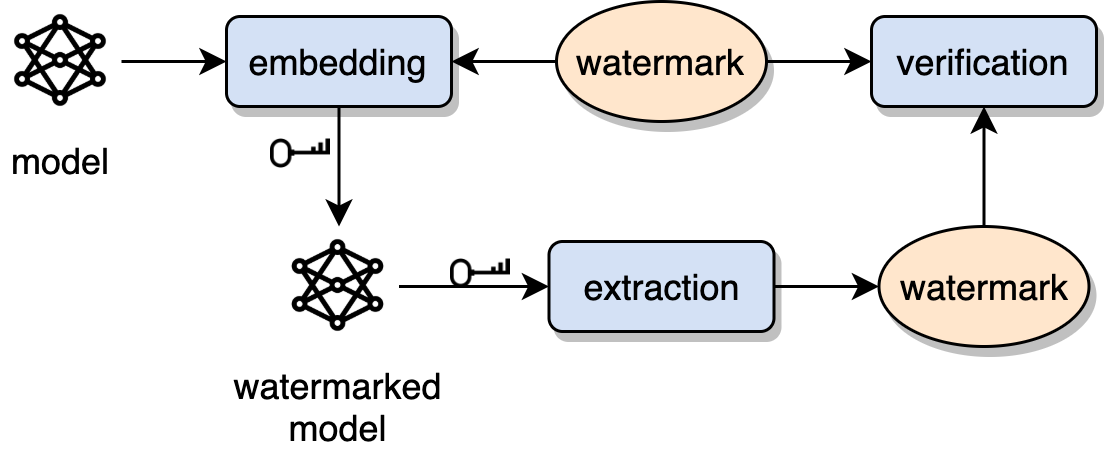
\includegraphics[width= 0.7\linewidth]{images/watermarking_workflow.png}
    \caption{A typical watermarking workflow}
    \label{fig:watermarking_workflow}
\end{figure}

\section{Fingerprinting}
We can consider fingerprinting as an extension of watermarking. While watermarking has the purpose to verify the \textit{owner} of a digital resource, fingerprinting wants to further trace back to the \textit{(malicious) recipient} of the resource. Therefore, fingerprinting techniques should be capable of embedding multiple, but unique, fingerprints in order to identify the recipient. These multiple fingerprints may be embedded in the same model, or in different versions of the model before distributing it.
%
Similar to watermarking, fingerprinting is already widely used in multimedia areas like images, audio and video \cite{lach_fpga_1998}, % Researchers extended the idea also to 
relational databases \cite{yingjiu_li_fingerprinting_2005}, and other digital data types.



%TODO: as discussed, move to a later section; also, distinguish between the concrete attacks that you have here, vs. what you call attacks in chapter 5 (SotA); in chapter 5, you rather have the *goal/aim* of the attack (or maybe the class), and here you have a specific attack (instance) (that might also achieve multiple goals at the same time..)
%----> done

%\section{Attacks}
%One of the most important requirements for a watermarking method is robustness (cf. \cref{sec:requirements}). In order to test robustness of the considered watermarking methods, we will perform two attacks, namely \textit{Fine-Tuning} and \textit{Parameter Pruning}. We have chosen those attacks, because a) these are the most common attacks performed in related work, and b) these are common steps to take when using a pre-trained model, e.g. in a transfer learning setting. A model user, regardless of whether malicious or not, could use fine-tuning for transferring the model to their task, and parameter pruning to compress the model.

%\subsubsection{Fine-Tuning}
% https://ruder.io/transfer-learning/
% https://machinelearningmastery.com/transfer-learning-for-deep-learning/
% https://medium.com/@14prakash/transfer-learning-using-keras-d804b2e04ef8
% https://builtin.com/data-science/transfer-learning

% Karen Simonyan and Andrew Zisserman. 2015. Very deep convolutional net- works for large-scale image recognition. In Proc. of ICLR.

%Transfer learning: Maxime Oquab, Leon Bottou, Ivan Laptev, and Josef Sivic. 2014. Learning and transferring mid-level image representations using convolutional neural net- works. In Proceedings of the IEEE conference on computer vision and pattern recognition.
%Some watermarking methods use fine-tuning \cite{girshick_rich_2014} to embed a watermark in a pre-trained model. Fine-tuning can be also seen as potential threat for the embedded watermark. Fine-Tuning can be either a targeted attack or an accidental attack: the attacker could perform fine-tuning for the purpose of Transfer Learning, or for purposely trying to remove the watermark by training on non-watermarked data. We will test the watermarking methods on the robustness against fine-tuning attacks 

%a model means that an already trained model is trained further on additional data with a smaller learning rate, usually for the purpose of Transfer Learning. In watermarking, some watermarking methods use fine-tuning to embed a watermark in a pre-trained model. We will mainly use fine-tuning as an attack and test the robustness of the watermarking methods, as we expect the (malicious) user to perform fine-tuning either for transfer learning or for purposely trying to remove the watermark. \red{CITE}

%\subsubsection{Parameter pruning}
% Song Han, Jeff Pool, John Tran, and William Dally. 2015. Learning both weights and connections for efficient neural network. In Advances in Neural Information Processing Systems. 1135–1143.



\chapter{Taxonomy of IPP for ML models}
\label{ch:taxonomy}

% ------ IPP overview figure
\begin{figure*}[t]

\begin{tikzpicture}
\node[inner sep=0pt] (overview) at (0,0) {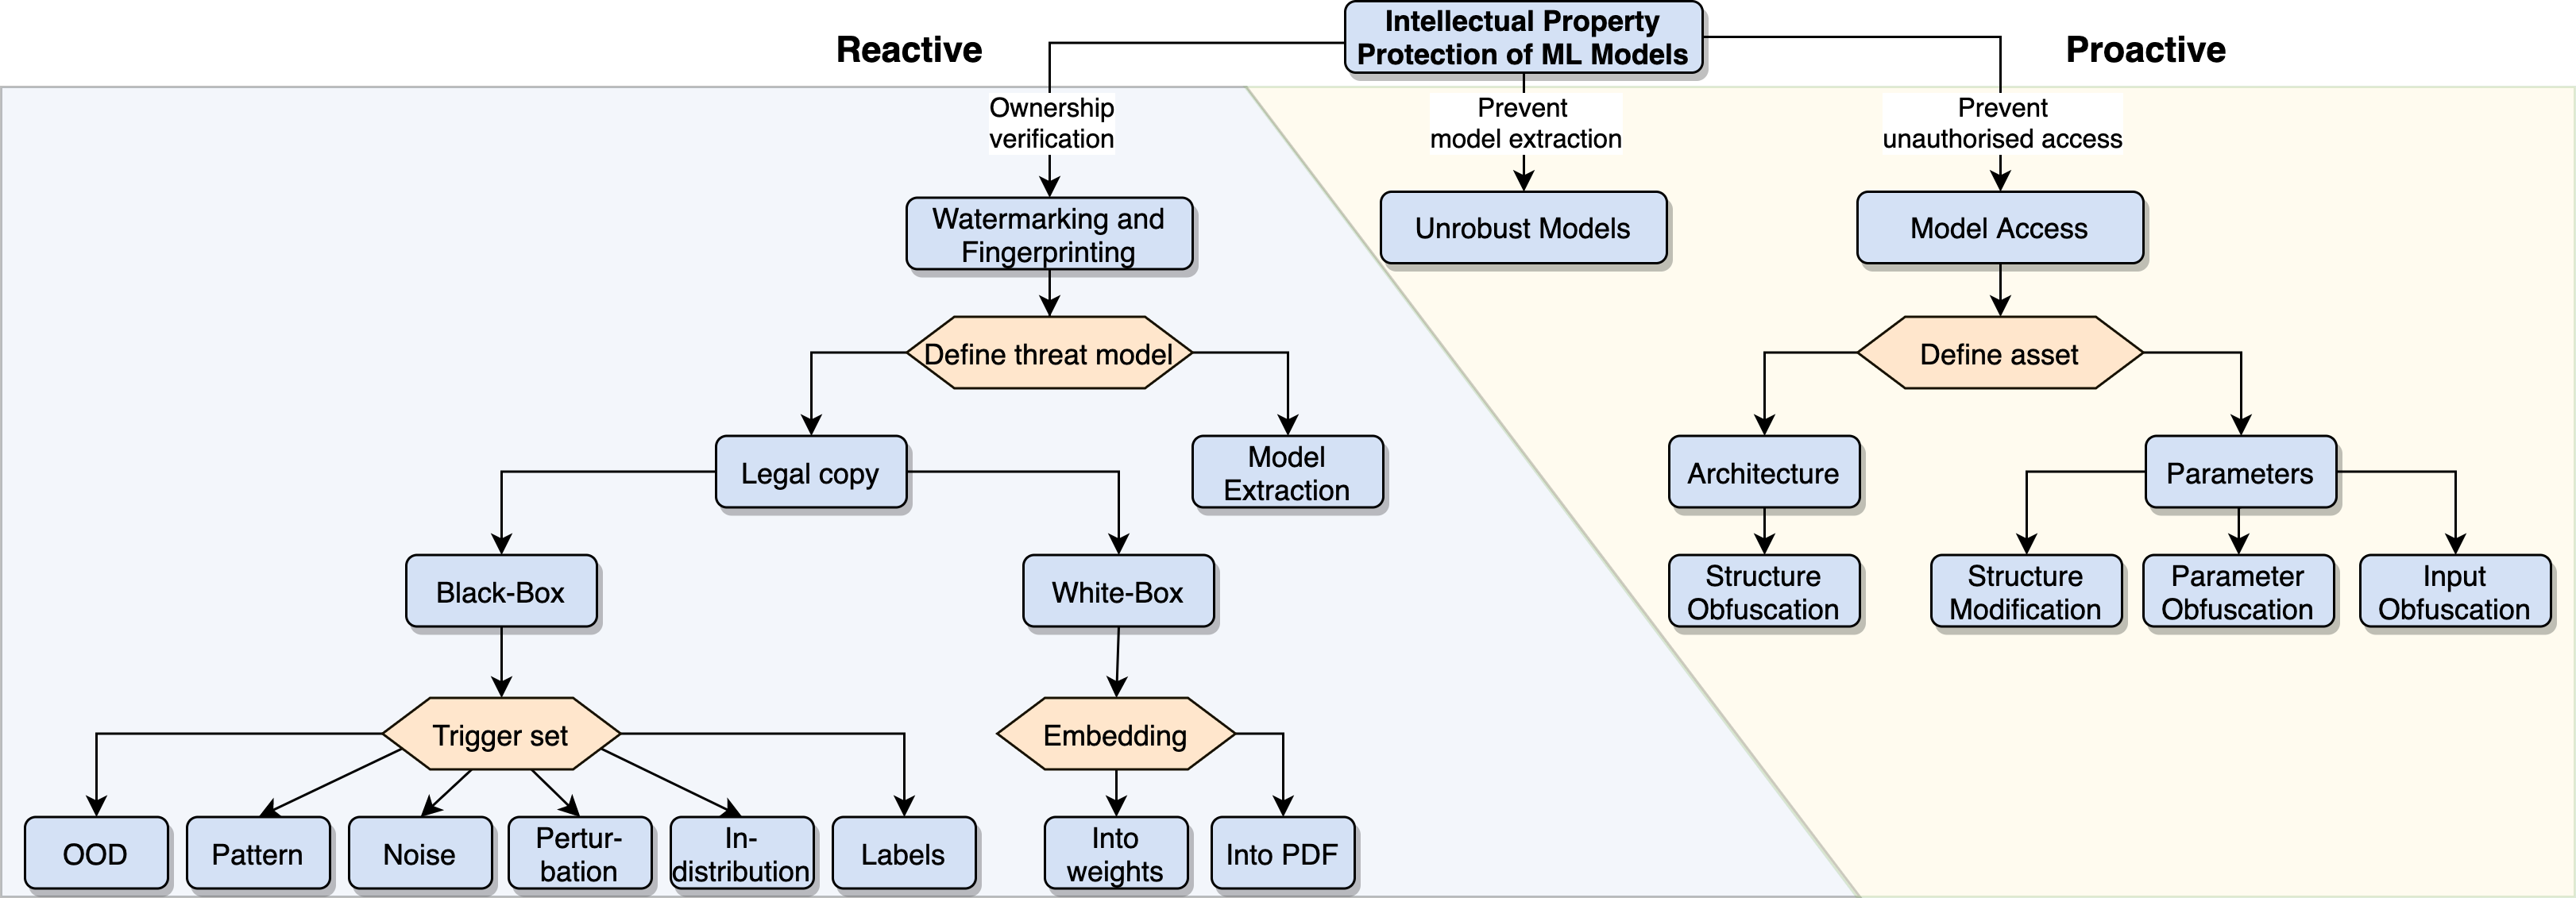
\includegraphics[width=\textwidth]{images/IPP_overview.png}};
%OOD:
\node[inner sep=0pt] (cite1) at (-8.65,-3.25) {\tiny \cite{adi_turning_2018}};
\node[inner sep=0pt] (cite2) at (-8.4,-3.25) {\tiny \cite{zhang_protecting_2018}};
\node[inner sep=0pt] (cite22) at (-8.1,-3.25) {\tiny \cite{yang_effectiveness_2019}};
%pattern:
\node[inner sep=0pt] (cite3) at (-7.7,-3.25) {\tiny \cite{zhang_protecting_2018}};
\node[inner sep=0pt] (cite4) at (-7.4,-3.25) {\tiny \cite{li_piracy_2020}};
\node[inner sep=0pt] (cite5) at (-7.1,-3.25) {\tiny \cite{guo_watermarking_2018}};
\node[inner sep=0pt] (cite6) at (-6.8,-3.25) {\tiny \cite{guo_evolutionary_2019}};
%noise:
\node[inner sep=0pt] (cite7) at (-6.25,-3.25) {\tiny \cite{zhang_protecting_2018}};
\node[inner sep=0pt] (cite8) at (-5.95,-3.25) {\tiny \cite{zhu_secure_2020}};
%perturbation:
\node[inner sep=0pt] (cite9) at (-5.3,-3.25) {\tiny \cite{merrer_adversarial_2019}};
\node[inner sep=0pt] (cite10) at (-5.0,-3.25) {\tiny \cite{li_how_2019}};
\node[inner sep=0pt] (cite11) at (-4.7,-3.25) {\tiny \cite{chen_blackmarks_2019}};
\node[inner sep=0pt] (cite12) at (-5.1,-3.45) {\tiny FP: \cite{zhao_afa_2019}};
\node[inner sep=0pt] (cite13) at (-4.7,-3.45) {\tiny \cite{lukas_deep_2020}};
%in-distr.:
\node[inner sep=0pt] (cite14) at (-3.85,-3.25) {\tiny \cite{namba_robust_2019}};
%trigger labels:
\node[inner sep=0pt] (cite15) at (-3,-3.25) {\tiny \cite{zhong_protecting_2020}};
\node[inner sep=0pt] (cite16) at (-2.7,-3.25) {\tiny \cite{zhang_deeptrigger_2020}};
\node[inner sep=0pt] (cite16) at (-2.4,-3.25) {\tiny \cite{xu_identity_2020}};

%into weights:
\node[inner sep=0pt] (cite17) at (-1.65,-3.25) {\tiny \cite{uchida_embedding_2017}};
\node[inner sep=0pt] (cite18) at (-1.35,-3.25) {\tiny \cite{wang_robust_2020}};
\node[inner sep=0pt] (cite19) at (-1.05,-3.25) {\tiny \cite{wang_watermarking_2020}};
\node[inner sep=0pt] (cite20) at (-0.75,-3.25) {\tiny \cite{feng_watermarking_2020}};
%into pdf:
\node[inner sep=0pt] (cite21) at (-0.3,-3.25) {\tiny \cite{rouhani_deepsigns_2019}};
\node[inner sep=0pt] (cite22) at (0.2,-3.25) {\tiny FP: \cite{chen_deepmarks_2019}};
%Model Extraction:
\node[inner sep=0pt] (cite23) at (1,-1.4) {\tiny \cite{jia_entangled_2020}}; 
\node[inner sep=0pt] (cite24) at (1.3,-1.4) {\tiny \cite{szyller_dawn_2020}};
% man könnte noch diese hinzufügen, aber lasse ich für die version erstmal...
%\node[inner sep=0pt] (cite241) at (1.6,-1.4) {\tiny \cite{wu_watermarking_2020}};
%\node[inner sep=0pt] (cite242) at (1.9,-1.4) {\tiny \cite{zhang_model_2020}};

% Unrobust models
 \node[inner sep=0pt] (cite25) at (1.7,1.15) {\tiny \cite{szentannai_preventing_2019}};
 
%Structure Obfuscation:
\node[inner sep=0pt] (cite101) at (3.35,-1.4) {\tiny \cite{xu_deepobfuscation_2018}};
 
% Structure Modification:
\node[inner sep=0pt] (cite102) at (5.2,-1.4) {\tiny \cite{fan_rethinking_2019}};

% Parameter Encryption & Obfuscation:
\node[inner sep=0pt] (cite103) at (6.13,-1.4) {\tiny \cite{gomez_security_2019}};
\node[inner sep=0pt] (cite104) at (6.43,-1.4) {\tiny \cite{chakraborty_hardware-assisted_2020}};
\node[inner sep=0pt] (cite105) at (6.73,-1.4) {\tiny \cite{alam_deep-lock_2020}};
\node[inner sep=0pt] (cite106) at (7.03,-1.4) {\tiny \cite{tang_deep_2020}};
\node[inner sep=0pt] (cite107) at (7.33,-1.4) {\tiny \cite{lin_chaotic_2020}};

%Input Obfuscation:
\node[inner sep=0pt] (cite108) at (8.1,-1.4) {\tiny \cite{aprilpyone_training_2020}};
\node[inner sep=0pt] (cite109) at (8.4,-1.4) {\tiny \cite{chen_protect_2018}};

\end{tikzpicture}

%    \caption{Taxonomy of IPP protection mechanisms for ML models.}
    \caption{Taxonomy of Intellectual Property Protection mechanisms for Machine Learning models. Note: not all considered papers are referenced in this diagram.}
        \label{fig:overview}
\end{figure*}
% ------ end

In this section, we provide a comprehensive taxonomy of IPP methods for ML models, the threat model and attacks.

We first define our threat model, to then discuss potential schemes to mitigate risks of those threats.
We then provide an overview of attacks against those IPP mechanisms.

\section{Threat Model}
\label{sec:threatmodel}

To define a threat model we first need to understand the motives of an attacker (or adversary or malicious user).
The model owner, i.e. the person that invested resources to obtain an ML model for a specific task, wants to offer the model to some target audience for use.
The most prominent reasons for an attacker to redistribute such a model would be (i) having no (or not enough) training data, expertise, time or computational power to train such a model themself, and/or (ii) the unwillingness to agree with the license terms of the obtained model or the fees for using it in a Machine Learning as a Service (MLaaS) setting.
We call the model that has to be protected the \textit{target model}, and the attacker's model, which arises from the target model, the \textit{adversary model}. As a threat model, we consider either one of the following situations:
% 
\begin{enumerate}
    \item \textbf{Legal copy:} The model owner distributes the model publicly, either for free, e.g. via a platform such as Model Zoo \cite{noauthor_model_nodate}, but with a restrictive license, or for a fee. The attacker then obtains this model and redistributes it via a lucrative API service.
    \item \textbf{Illegal copy:} The model owner distributes the model as a pay-per-query API service. The attacker then performs a Model Extraction Attack and provides his own lucrative API service.
\end{enumerate}

Regardless of how the attacker obtained the model, in both cases, the IP of the model owner is illegally utilised. For both cases, we will discuss methods to protect the IP of the model owner. It is important to differentiate between those two cases, as this has a large impact on selecting potential defence mechanisms. 

\section{IPP Methods}
We developed a comprehensive taxonomy of IPP methods for ML models, depicted in \cref{fig:overview}.

A principal categorisation of model watermarking methods is by \textit{white-box} or \textit{black-box} watermarking methods. White-box approaches embed the watermark in the model parameters or other model characteristics. With that in mind, the model owner would need the get the stolen copy from the attacker for the watermark verification process. This scenario seems unrealistic in most settings (e.g. an attacker offering an API service based on the model never discloses the model itself), and is the likely reason why black-box watermarking tends to be more popular, as the model owner can verify ownership with as little as a set of trigger inputs and the corresponding responses of the adversary model.

A further distinction is between (i) \textit{reactive methods}, which try to react to a threat event, or (ii) \textit{proactive methods}, which means the defender takes initiative, to prevent a threat event.
%Reactive methods include watermarking and fingerprinting, while proactive methods include model access control.
Regarding the goal of the protection, we distinguish methods that enable to verify the ownership of a model, by \textit{model watermarking} and \textit{model fingerprinting}, and are thus \textit{reactive}, and methods that, e.g., want to prevent unauthorised model access, and are thus \textit{proactive}. %TODO: Mimosanet
Ownership verification is a weak form of protection, as it requires the unauthorised usage of the model to be known (or at least suspected), and further requires some form of access to the model. Model access control, on the other hand, shall prevent such illegal use, by rendering the model useless to unauthorised users. This is comparable to preventing unauthorised use of, e.g., software.

Watermarking against the threat of a model extraction attack is mostly achieved by special black-box watermarking techniques that survive such an attack, i.e. the hidden information is "stolen" along with the model itself. In case a user initially obtained a legal copy of the ML model but is then using it in a way not according to the licensing terms, more techniques are available. White-box approaches for this case embed the ownership information directly into the model parameters, or in their probability density function (PDF). Black-box approaches mostly rely on specific input samples, so-called \textit{trigger sets}, that will cause the model to behave in a way that is unexpected for the task, and unknown to the attacker. The techniques mainly differ in the way these triggers are constructed.

Model access control methods can be distinguished by the asset they want to protect. Most work focuses on the protection of the model parameters, either by encryption, other obfuscation techniques, or requiring a specific method to transform the inputs. If the model structure (or architecture) is to be protected, obfuscation techniques for those are employed.

\section{Attack Model} \label{sec:attack-model}
%TODO: make more generic, for all IPP

In \cref{sec:attacks} we will introduce specific attacks against IPP mechanisms, namely \textit{detection}, \textit{overwriting}, \textit{invalidation} and \textit{removal}. Therefore, this section provides the attack models to which we will refer later on. Let us assume that the attacker obtains a legal copy of the target model, and either knows or assumes that the model has an IPP in place.

We consider the following cases as attack models for watermarking:

\begin{itemize}
    \item  
\textbf{Watermark detection:} The attacker wants to detect if there is a watermark in the model, e.g. to then perform a targeted watermark removal or overwriting. If the watermark is not secured with an additional mechanism (e.g. a private key for extraction), the attacker could also claim ownership.
\item \textbf{Watermark overwriting:} The attacker wants to overwrite an existing watermark by placing their own watermark and making the model owner's watermark useless.
\item \textbf{Watermark invalidation:} The attacker wants to disable the watermark function, without actually removing it from the model, so that it cannot be verified. 
%\footnote{An example is an ensemble attack where API services do not respond relying on a single model's prediction, but on several different models so that when triggering, the expected trigger label is not revealed \cite{hitaj_evasion_2019}.}
\item \textbf{Watermark removal:} The attacker wants to modify the model in a way such that the model owner's watermark extraction algorithm will no longer result in proving correct ownership, ownership of the real model owner.
\end{itemize}

Most of these attacks are also valid against \textit{fingerprinting}.

Against \textbf{model access control} mechanisms, an attacker mostly would want to \textbf{remove} or \textbf{invalidate} (or potentially overwrite) the mechanism to gain unauthorised access to use the model (as black-box) or to reveal either the model architecture or model parameters for other purposes.


\chapter{State of the Art: Model Watermarking, Fingerprinting and Attacks}
\label{ch:sota}

%In order to prove ownership the watermarking method has to have a low false positive rate. Suppose that we allow at most $\Delta$ misclassifications among $N$ trigger images. Assuming independence between the classification of each trigger image, we can calculate the probability of successful watermark verification by
%\begin{align*}
%    \mathrm{Pr} = \sum_{\delta = 0}^{\Delta} \begin{pmatrix} N \\ \delta
%    \end{pmatrix} (1-\rho)^{\delta}\rho^{N-\delta},
%\end{align*}
%with $\rho$ being the accuracy of the model on the trigger set \cite{guo_evolutionary_2019, rouhani_deepsigns_2019, guo_watermarking_2018}.

% Isabell: nicht low false negative rate?
% Rudi: Ja, ein false positive hält einen nicht davon ab, ownership zu zeigen. Eigentlich ist es aber wohl besser zu sagen, dass beides niedrig sein muss. Weil wenn ich nur TN niedrig haben will und das ausreicht, kann man einen sehr trivialen detector bauen, der immer richtig ist...

There are several connotations of watermarking, and generally, information hiding, along the machine learning process, as depicted in \cref{fig:watermarking-ml-process}.
% TODO: There was another paper with a similiar idea
Sablayrolles et al. \cite{sablayrolles_radioactive_2020} propose a technique that \textit{traces data usage}; it marks (training) data in a special way, so that a ML model trained on that data will bear a watermark that can be identified  (cf. \circled{1} in \cref{fig:watermarking-ml-process}).
The main body of work, and the focus of this section, consider ML models as the objects that need protection and in which the watermark is embedded  (cf. \circled{2} in \cref{fig:watermarking-ml-process}).
Abdelnabi et al. \cite{abdelnabi_adversarial_2020} propose a special form of watermarking. Their scheme is not watermarking a \textit{model}, but the \textit{output} of a text generating model (cf. \circled{3} in \cref{fig:watermarking-ml-process}). They assume that an attacker could use the model for generating whole articles. In such a case, the watermark can be extracted from the generated text and prove the illegitimate usage of the model.
In some settings, it is further considered that a marked output (prediction, or data) is generated with the explicit goal to trace the usage of this data, e.g. for training by an attacker (cf. \circled{4} in \cref{fig:watermarking-ml-process}). This is a special form of \circled{1}, as the data origin is different, and of \circled{2}, as the adversary model is \textit{implicitly marked} (cf. %. Most methods following this approach are described in 
\cref{sec:wm:countering_extraction}).

We want to point out that information hiding techniques for ML models may have other applications than watermarking. For instance, Song et al. \cite{song_machine_2017} propose a technique to hide data from a private training dataset in the internals of a model (e.g. the weights) trained upon said dataset. 
This way, an attacker that does not have direct access to the training data, but can only let their model be trained on the data by the data owner, can exfiltrate this data via the derived machine learning model, i.e. perform a data exfiltration attack  (cf. \circled{5} in \cref{fig:watermarking-ml-process}).
We, however, consider techniques which hide information about a lawful owner of the model. 
\begin{figure}
\centering
    % ------ ML process overview figure

\begin{tikzpicture}
\node[inner sep=0pt] (mlProcess) at (-2.1,0) {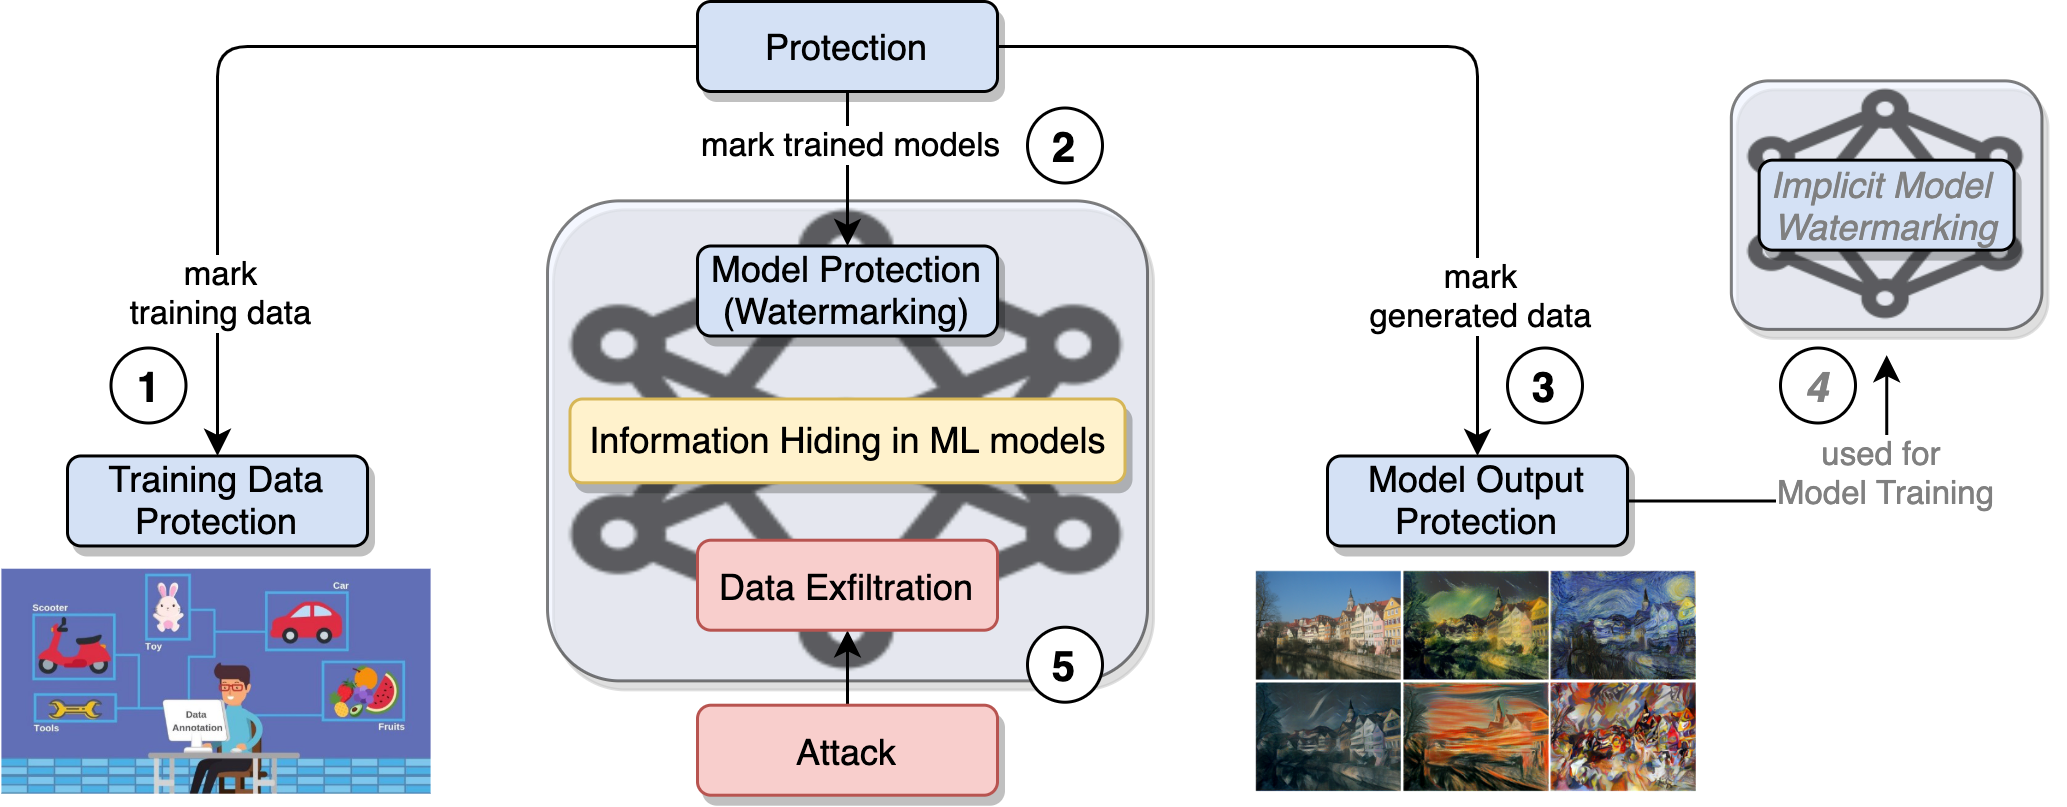
\includegraphics[width=\linewidth]{images/Watermarking_aspects.png}};

%MarkTrainingData:
\node[inner sep=0pt] (cite200) at (-7.5,0.1) {\tiny \cite{sablayrolles_radioactive_2020}};
%MarkOutputData:
% marks output, doesn't talk about model training
\node[inner sep=0pt] (cite211) at (0.7,0.1) {\tiny \cite{abdelnabi_adversarial_2020}};

%specifically for model training!
\node[inner sep=0pt] (cite212) at (4.5,0.35) {\tiny \cite{szyller_dawn_2020}};

% marks all output for surrogate model training
\node[inner sep=0pt] (cite213) at (4.5,0.1) {\tiny \cite{zhang_model_2020}};
\node[inner sep=0pt] (cite214) at (4.5,-0.15) {\tiny \cite{wu_watermarking_2020}};
%OtherInformationHiding
\node[inner sep=0pt] (cite225) at (-2.5,-1.8) {\tiny \cite{song_machine_2017}};
\end{tikzpicture}
    \caption{Different notions of information hiding along a ML process}
    \label{fig:watermarking-ml-process}
\end{figure}

The vast majority of watermarking methods for ML models is designed specifically for DNNs. The main reason for this is not only the high value of DNNs, as they require large datasets and long training time, but also the number of "degrees of freedom" in a DNN. Large DNNs thus have, compared to other ML models, more "space" for hiding marks. 
Most authors evaluate the schemes on image classification task. However, some authors extend the methods to other tasks, like audio classification \cite{jia_entangled_2020}, image captioning \cite{lim_protect_2020}, image processing \cite{quan_watermarking_2020, wu_watermarking_2020, zhang_model_2020} (where the output is an image/data, rather than a prediction), or specific learning settings, such as GANs \cite{skripniuk_black-box_2020}, Federated Learning with DNNs \cite{atli_waffle_2020},
%\footnote{Preceding master thesis in \cite{xia_watermarking_2020}}
Graph Neural Networks \cite{zhao_watermarking_2020}, and Deep Reinforcement Learning \cite{behzadan_sequential_2019}.

\section{Requirements} \label{sec:requirements}
A watermarking scheme should fulfil a couple of requirements. Literature is not coherent in the naming of these requirements of watermarking (and fingerprinting) methods, and we, therefore, aim at providing a common nomenclature. 
To this end, we collect all the requirements that were proposed in the papers included in our literature review and list them in \cref{tab:requirement}, identifying also terms used as synonyms, along with references to the respective publications.

\begin{table*}[t]
\centering
% No punctuation in last sentence + caption should be set as an inverted pyramid. see IEEE editorial style manual: http://journals.ieeeauthorcenter.ieee.org/wp-content/uploads/sites/7/IEEE-Editorial-Style-Manual_081920.pdf
\caption{Requirements for Watermarking techniques. The notation is not consistent throughout the papers, but the terms in the left column are the most prominent ones. These requirements mostly apply also to Fingerprinting methods}
%  \begin{adjustbox}{width=1.0\textwidth,center=\textwidth}

\rowcolors{2}{gray!15}{white}

\begin{tabular}{|p{0.15\textwidth}|p{0.4\textwidth}|p{0.4\textwidth}|}
\rowcolor{gray!15}
\hline
\textbf{Property}               & \textbf{Description}                                                                                              & \textbf{Other terms used in papers}                        \\ \hline
%
Effectiveness                   & The model owner should be able to prove ownerhsip anytime and multiple times if needed                            & Authentication \cite{li_piracy_2020}, Functionality \cite{li_how_2019}                              \\ \hline
%
Fidelity                        & The accuracy of the model should not be degraded after embedding the watermark                                    & Funcionality-preserving \cite{li_piracy_2020, wang_robust_2020, adi_turning_2018}, Loyalty \cite{merrer_adversarial_2019}, Utility \cite{szyller_dawn_2020}
\scriptsize{(Image WM: Transparency \cite{potdar_survey_2005}; Relational Data WM: Usability \cite{kamran_comprehensive_2018})}                \\ \hline
%
Robustness                      & The embedded watermark should resist a designated class of transformations                                        & Unremovability \cite{adi_turning_2018, szyller_dawn_2020}                                            \\ \hline
%
Security                        & The watermark should be secure against brute-force or specifically crafted evasion attacks                        & Secrecy \cite{skripniuk_black-box_2020}, Unforgeability \cite{adi_turning_2018, wang_robust_2020}                                    \\ \hline
%
Legality                        & An adversary cannot produce a watermark for a model that was already watermarked by the model owner               & Ownership piracy resilient \cite{adi_turning_2018, wang_robust_2020}, Non-ownership piracy \cite{szyller_dawn_2020}           \\ \hline
%
Integrity                       & The watermark verification process should have a negligible false positive rate                                   & Low false positive rate \cite{guo_evolutionary_2019, guo_watermarking_2018}, Non-trivial ownership \cite{li_piracy_2020, adi_turning_2018, wang_robust_2020}, Uniqueness \cite{quan_watermarking_2020} \\ \hline
%
Reliability                     & The watermark verification process should have a negligible false negative rate                                   & Credibility \cite{chen_blackmarks_2019}                                                \\ \hline
%
Efficiency                      & The watermarking embedding and verification process should be fast                                                &                                                            \\ \hline
%
Capacity                        & The watermarking scheme should be capable of embedding a large amount of information                              & Payload \cite{guo_watermarking_2018}                                                    \\ \hline
%


% \hline
% \textbf{Property}     & \textbf{Description}                                                                                    & \textbf{Other terms used in papers}                        \\ \hline
% Fidelity              & The accuracy of the model should not be degraded after embedding the watermark                          & Funcionality-preserving \cite{li_piracy_2020, wang_robust_2020, adi_turning_2018}, Loyalty \cite{merrer_adversarial_2019}, Utility \cite{szyller_dawn_2020}
% \scriptsize{(Image WM: Transparency \cite{potdar_survey_2005}; Relational Data WM: Usability \cite{agostino_cortesi_watermarking_2010})}       \\ \hline
% Robustness            & The embedded watermark should resist a designated class of transformations                        & Feasibility \cite{li_how_2019}                                      \\ \hline
% Non-trivial ownership & An adversary should not be able to claim ownership of the watermarked model without knowing the watermark        &                                                  \\ \hline
% Legality              & An adversary cannot produce a watermark for a model that was already watermarked by the model owner                        & Ownership piracy resilient \cite{adi_turning_2018}, non-ownership piracy \cite{szyller_dawn_2020} \\ \hline
% Reliability           & The watermark verification process should have a negligible false negative rate                         & Credibility \cite{chen_blackmarks_2019}                               \\ \hline
% Integrity             & The watermark verification process should have a negligible false positive rate                         & Low false positive rate \cite{guo_evolutionary_2019, guo_watermarking_2018}  \\ \hline
% Capacity              & The watermarking scheme should be capable of embedding a large amount of information                  & Payload \cite{guo_watermarking_2018}                                     \\ \hline
% Efficiency            & The watermarking embedding and verification process should be fast &                                                  \\ \hline
% Effectiveness         & The model owner should be able to prove ownerhsip anytime and multiple times if needed                                                                  & Authentication \cite{li_piracy_2020}                                   \\ \hline
% Security              & The watermark should be secure against brute-force or specifically crafted evasion attacks                                  & Unremovability \cite{szyller_dawn_2020, adi_turning_2018}                             \\ \hline


\end{tabular}
% \end{adjustbox}
\label{tab:requirement}
\end{table*}

%TODO? Tamper-resistance?
%Tamper resistance:  Tamper-detection watermarking was developed to check the authenticity of digital photographs.  Watermarks of  this  type  are  sensitive  to  any change of  the content data;  thus,  by  checking  the integrity  of the  watermark,  the  system  can  determine whether or not the content has the ever been modified or replaced
 

The most important %and obvious 
requirements are  \textbf{effectiveness}: the watermark shall be embedded in a way that the model owner can prove ownership anytime, \textbf{fidelity}: the model's accuracy shall not be degraded because of the watermark embedding, and \textbf{robustness}: the watermark embedding should be robust against several kinds of attacks, including fine-tuning, model compression and other, specifically crafted attacks.
%
The remaining requirements are listed in \cref{tab:requirement}. 
% Other important requirements are \textbf{security}: the watermark shall be secure against brute-force and evasion attacks,  \textbf{legality}: the adversary shall not be able to watermark an already watermarked model, \textbf{integrity}: the watermark embedding shall yield to minimal false positive rate, \textbf{reliability}: the watermark embedding shall yield to a minimal false negative rate, \textbf{efficiency}: the watermarking scheme shall have a minimal overhead, \textbf{capacity}: the watermark should be able to carry a lot of information.
% end candidate for deletion
Note, that non-trivial ownership is sometimes used as a synonym for integrity, meaning that innocent models are not being accused of ownership piracy, but also as a requirement that an attacker cannot easily claim ownership without knowing the watermarking scheme and embedded watermark. Moreover, authentication is more a subset of effectiveness than a real synonym since it only requires that there is a provable association between an owner and their watermark. \textbf{Feasibility} is used as a combination of robustness and effectiveness \cite{li_how_2019}, and \textbf{correctness} as a combination of effectiveness, reliability, and integrity \cite{lukas_deep_2020}. Fingerprinting should fulfil two more requirements: \textbf{uniqueness} -- the fingerprint can be uniquely identified with the user, and \textbf{scalability} -- the fingerprinting scheme should be able to embed multiple fingerprints, either in the same model or in multiple versions of the model. A fingerprinting method that embeds multiple fingerprints, e.g. \cite{chen_deepmarks_2019}, could not only trace back the attacker but also identify collaboration between several malicious users.
 
\begin{sidewaystable}
    \centering

\caption{Requirements met by watermarking and fingerprinting schemes.  We distinguish two degrees:
%$\sim$ indicates a claim -- the authors of the scheme claim that the scheme fulfils this property; \checkmark indicates a demonstration -- the authors show empirically that the property is fulfilled
$\sim$ indicates: the respective authors claim the scheme fulfils this property; \checkmark indicates: the authors show empirically that the property is fulfilled
}

\rowcolors{2}{white}{gray!15}

\setlength\tabcolsep{2pt}
\setlength\extrarowheight{5pt}

\begin{tabular}{|l|c|c|c|c|c|c|c|c|c|c|c|c|c|c|c|c|c|c|c|c|c|c|c|c|c|c|c|c|c|c|c|}
\rowcolor{gray!15}
\hline
 & \multicolumn{7}{l|}{\textbf{white-box}}                                                                             & \multicolumn{24}{l|}{\textbf{black-box}}                                                                                                                                                                                                                                                                                                                                                                 \\ \cline{2-32} 
%                                     & \multicolumn{2}{l|}{\textbf{into pdf}} & \multicolumn{4}{l|}{\textbf{into weights}}                   & \textbf{?} & \textbf{OOD, pattern, noise} & \textbf{OOD} & \textbf{pattern} & \textbf{}         &                   &        & \multicolumn{5}{l|}{\textbf{perturbation}}           & \textbf{in-distr} & \multicolumn{2}{l|}{\textbf{aginst ME}} & \multicolumn{3}{l|}{\textbf{labels}} & \multicolumn{4}{l|}{\textbf{extending existing work}}          & \multicolumn{3}{l|}{\textbf{image processing}}            \\ \hline
%
\hline
\multicolumn{1}{|l|}{\textbf{Property}}      & {\tiny\cite{rouhani_deepsigns_2019}}         & {\tiny\cite{chen_deepmarks_2019}}      & {\tiny\cite{uchida_embedding_2017}}     & {\tiny\cite{wang_robust_2020}} & {\tiny\cite{wang_watermarking_2020}} & {\tiny\cite{feng_watermarking_2020}}       & {\tiny\cite{chen_specmark_2020}}   & {\tiny\cite{zhang_protecting_2018}}                        & {\tiny\cite{adi_turning_2018}}          & {\tiny\cite{li_piracy_2020}}       & {\tiny\cite{guo_watermarking_2018}} & {\tiny\cite{guo_evolutionary_2019}} & {\tiny\cite{zhu_secure_2020}}    & {\tiny\cite{merrer_adversarial_2019}} & {\tiny\cite{li_how_2019}} & {\tiny\cite{chen_blackmarks_2019}}  & {\tiny\cite{zhao_afa_2019}} & {\tiny\cite{lukas_deep_2020}} & {\tiny\cite{namba_robust_2019}}             & {\tiny\cite{szyller_dawn_2020}}       & {\tiny\cite{jia_entangled_2020}}                     & {\tiny\cite{zhong_protecting_2020}}     & {\tiny\cite{zhang_deeptrigger_2020}}    & {\tiny\cite{xu_identity_2020}}      & {\tiny\cite{yang_effectiveness_2019}}      & {\tiny\cite{guan_reversible_2020}} & {\tiny\cite{skripniuk_black-box_2020}} & {\tiny\cite{lim_protect_2020}} & {\tiny\cite{wu_watermarking_2020}}       & {\tiny\cite{zhang_model_2020}} & {\tiny\cite{quan_watermarking_2020}}       \\ \hline
\multicolumn{1}{|l|}{Effectiveness} & \checkmark      & \checkmark                 & \checkmark & \checkmark   &  \checkmark                   & \checkmark & \checkmark           & \checkmark                   & \checkmark   & \checkmark             & \checkmark              & \checkmark              & \checkmark   & \checkmark   & \checkmark    &   \checkmark          & \checkmark      & \checkmark    & \checkmark              & \checkmark          & \checkmark                    & \checkmark      & \checkmark           & \checkmark    & \checkmark      & \checkmark             & \checkmark             & \checkmark   & \checkmark             & \checkmark                &  \checkmark \\ \hline
\multicolumn{1}{|l|}{Fidelity}      & \checkmark            & \checkmark                 & \checkmark       & \checkmark         & \checkmark                & \checkmark       & \checkmark       & \checkmark                         & \checkmark         & \checkmark             & \checkmark              & \checkmark              & \checkmark   & \checkmark   & \checkmark    & \checkmark        & \checkmark   & \checkmark & \checkmark              & \checkmark          & \checkmark                    & \checkmark      & \checkmark           & \checkmark    & \checkmark      & \checkmark             & \checkmark             & \checkmark         & \checkmark                   &                     & \checkmark       \\ \hline
% \multicolumn{1}{|l|}{Robustness}    & FT, MC, OW      & FT, MC, OW           & FT, MC     & FT, MC, OW   & FT, MC              & FT, MC, OW & FT, MC, TL & FT, MC                       & FT, TL       & FT, MC           & $\sim$             & FT                & FA, TL & FT, MC & FT      & FT, MC , OW & FT, MC    & \checkmark    & FT, MC            & ME            & ME, MC, FT, NC, FP       & FT, MC    & FT, MC, OW     & MC      & FT, MC, D &                  & FT,  MC          & FT, MC       & cropping, adding noise & \checkmark                & FT, MC, OW \\ \hline
\multicolumn{1}{|l|}{Robustness}    & \checkmark & \checkmark & \checkmark & \checkmark & \checkmark & \checkmark & \checkmark & \checkmark & \checkmark & \checkmark & $\sim$ & \checkmark & \checkmark & \checkmark & \checkmark     & \checkmark & \checkmark & \checkmark    & \checkmark  & \checkmark  & \checkmark  & \checkmark & \checkmark  & \checkmark & \checkmark &                  & \checkmark & \checkmark & \checkmark & \checkmark & \checkmark \\ \hline
\multicolumn{1}{|l|}{Security}      & \checkmark            & \checkmark                 & $\sim$      & $\sim$        & $\sim$               &            & $\sim$      & \checkmark                         & $\sim$        &                  & \checkmark              &                   & \checkmark   & $\sim$  & \checkmark    & \checkmark        &           &         &                   &               &                         &           & \checkmark           &         &           &                  & \checkmark             &              & \checkmark                   &                     &            \\ \hline
\multicolumn{1}{|l|}{Legality}      &                 &                      &            & $\sim$        &                     &            &            &                              &              &                  &                   &                   &        &        & \checkmark    &             &           &         &                   & $\sim$         &                         &           &                &         &           &                  &                  &              &                        &                     &            \\ \hline
\multicolumn{1}{|l|}{Integrity}     & \checkmark            & \checkmark                 &            & \checkmark         &                     &            & \checkmark       &                              & \checkmark         & \checkmark             & \checkmark              & \checkmark              &        &        & \checkmark    & \checkmark        & \checkmark      & \checkmark    &                   &               &                         &           & \checkmark           &         &           &                  &                  &              &                        &                     &            \\ \hline
\multicolumn{1}{|l|}{Reliability}   & \checkmark            & \checkmark                 &            &              &                     &            & $\sim$      &                              &              &                  &                   &                   &        &        &         & \checkmark        & \checkmark      & \checkmark    &                   & \checkmark          &                         &           &                &         &           &                  &                  &              &                        &                     &            \\ \hline
\multicolumn{1}{|l|}{Efficiency}    & \checkmark            & \checkmark                 & $\sim$      &              & $\sim$               & \checkmark       & \checkmark       &                              &              &                  &                   &                   &        & $\sim$  &         & \checkmark        &           &         &                   & \checkmark          &                         & \checkmark      &                &         &           &                  &                  &              &                        &                     &            \\ \hline
\multicolumn{1}{|l|}{Capacity}      & \checkmark            &                      & \checkmark       &              & \checkmark                & \checkmark       &            &                              &              &                  & \checkmark              &                   &        &        &         & \checkmark        &           &         &                   &               &                         &           &                &         &           &                  & \checkmark             & \checkmark         & \checkmark                   &                     & $\sim$      \\ \hline
\end{tabular}

\label{tab:summary-req}

\end{sidewaystable}







We provide an overview of all the watermarking and fingerprinting schemes considered in this thesis, and whether they are meeting the above-mentioned requirements, in \cref{tab:summary-req}.
%, which is inspired by \cite{li_how_2019}. We extend their summary by incorporating the additional identified requirements, and from their initially considered seven schemes to the XX schemes investigated in this paper.
%TODO: describe what we can learn from this table.
We observe %from \cref{tab:summary-req} 
that all schemes fulfil the above-identified most important requirements of fidelity, effectiveness and integrity, except for \cite{guan_reversible_2020}, which on purpose gives up on robustness in favour of reversibility: the authors point out that the application of their scheme is not IPP, but integrity authentication, and that all existing watermarking methods are irreversible -- once the watermark is embedded, it cannot be removed to restore the original model without degrading the model's performance.
They argue that irreversible watermarking schemes are permanently modifying the model's internals, and thus destroying the integrity of the model, which could have severe consequences especially in applications for the medical or defence domain, etc.
%Therefore, the authors introduce the first reversible black-box watermarking scheme.
To make the scheme reversible they sacrifice the robustness requirement, inspired by traditional image integrity. % and Guan et al. adapted it to DNNs.
For Zhang et al.'s method \cite{zhang_model_2020}, the fidelity requirement does not apply since it is not well-defined for image processing. To determine for a model that outputs an image (or other complex data) whether a watermarked version of such a model is comparable to the original one, one would need to define a similarity measure to compare if the two outputs are equivalent.

Watermarking methods can be categorised into two main fields, \textit{white-box} and \textit{black-box} watermarking. White-box means that the model owner needs access to the stolen model's parameters or other model characteristics, in either step of the IPP method process, i.e. also during watermark extraction and verification. A black-box method generally only needs access to the model's prediction, e.g. via an API service, to observe matching input and output from the ML model, using it in a similar fashion as an \textit{oracle}. In the following sections, we discuss both of the watermarking types.

\begin{figure}
     \centering
     \begin{subfigure}[b]{0.7\textwidth}
         \centering
         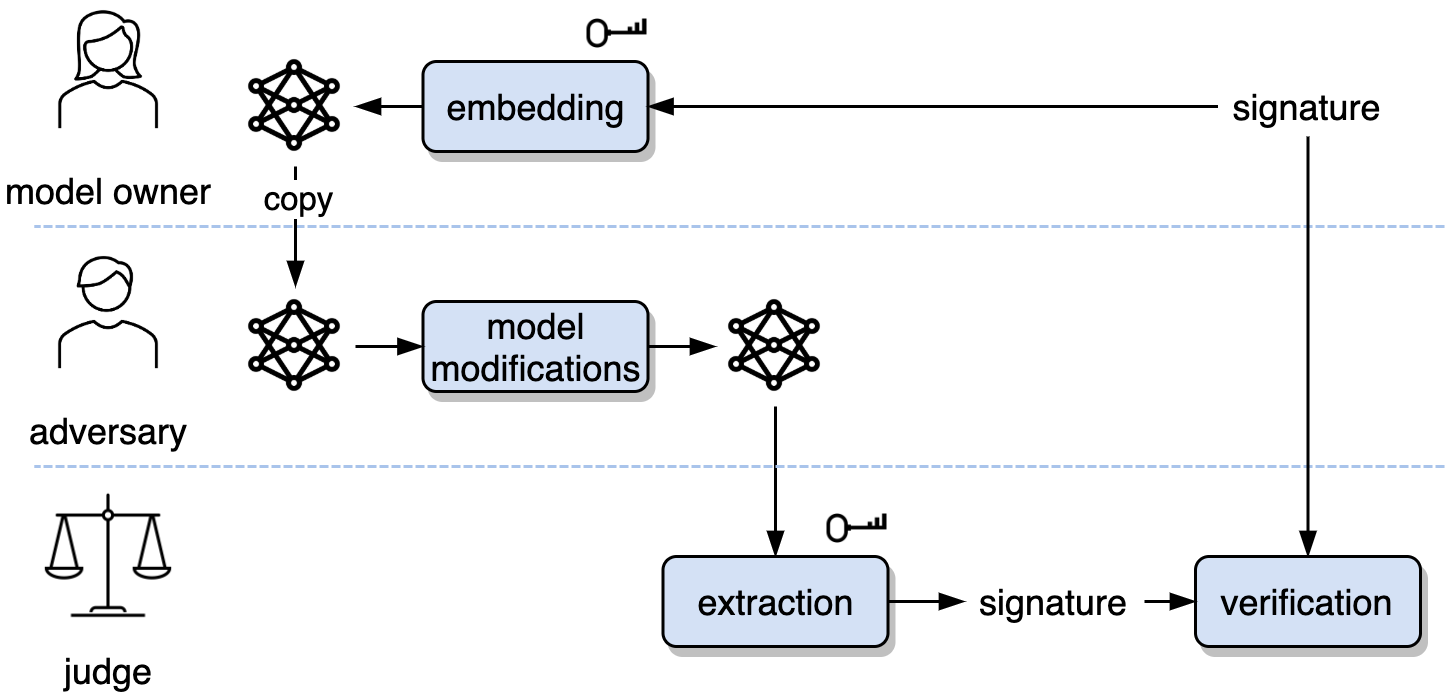
\includegraphics[width=\textwidth]{images/whitebox_workflow.png}
         \caption{}
         \label{fig:whitebox-workflow}
     \end{subfigure}
     \hfill
     \begin{subfigure}[b]{0.7\textwidth}
         \centering
         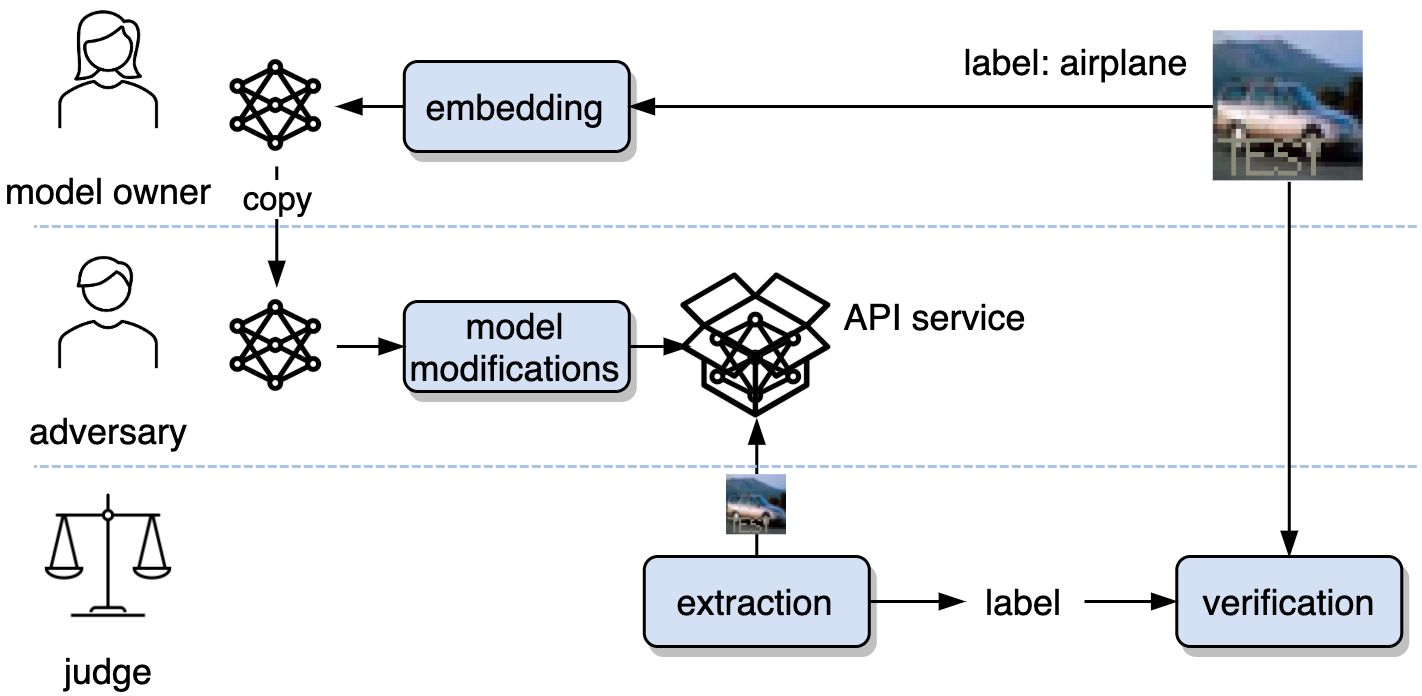
\includegraphics[width=\textwidth]{images/blackbox_workflow.png}
         \caption{}
         \label{fig:blackbox-workflow}
     \end{subfigure}
        \caption{Typical workflows for (a) white-box watermarking and (b) black-box watermarking}
        \label{fig:bothworkflows}
\end{figure}

\section{White-box Watermarking}
\label{sec:whitebox}
White-box watermarking requires full access to the model in order to verify the watermark. Usually, the model owner creates a $T$-bit signature vector $\mathbf{b} \in \{0,1\}^T$ that is a set of arbitrary binary strings that should be independently and identically distributed (iid) \cite{rouhani_deepsigns_2019}. This binary vector serves as a watermark and is usually embedded into the model by fine-tuning with regularisation. We call this type of embedding scheme \textit{regulariser based}. The general workflow for a regulariser based embedding scheme is illustrated in \cref{fig:whitebox-workflow}.

% --- regulariser based - into weights --- fingerprinting potential
The first framework for embedding a watermark into a DNN was proposed by Uchida et al. \cite{uchida_embedding_2017}\footnote{Slightly extended version in \cite{nagai_digital_2018}} in 2017. They follow the idea of embedding a signature into the model, particularly in the DNN's weights. 
While it would be possible to directly alter the model's parameters, as it would be done for watermarking relational data, this would degrade the model's performance.
%They point out that it would be possible to directly change the model's parameters but this would degrade the model's performance as they show experimentally and thus propose embedding the watermark while training the network. Furthermore, t
They thus describe three ways of embedding the watermark: while training, while fine-tuning, or by using the distilling approach \cite{hinton_distilling_2015}. The fine-tuning approach is especially interesting when the model owner wants to place individual watermarks (i.e. fingerprints) before distributing to different users, in order to trace back the recipient in case of copyright infringement (cf. \cref{sec:fingerprinting:user-specific-wm}). The model is trained with a regulariser term, given the signature $\mathbf{b} \in \mathbb{R}^T$, the averaged weights vector $\mathbf{w} \in \mathbb{R}^M$ and a specially crafted \textit{embedding matrix} $\mathbf{M} \in \mathbb{R}^{T \times M}$. The embedding matrix $\mathbf{M}$ can be considered a secret key for the embedding and extracting process. The watermark is extracted by applying $\mathbf{M} \in \mathbb{R}^{T \times M}$ to the weights vector $\mathbf{w} \in \mathbb{R}^M$ and then applying a step function:
\begin{align}
    \mathbf{\tilde b}_j = s(\sum_{i=1}^M \mathbf{M}_{ji}\mathbf{w}_i),
\end{align}
where $s(\cdot)$ is the unit step function. The resulting vector $\mathbf{\tilde b}$ is then compared with the signature $\mathbf{b}$ and the BER (bit error rate) is computed. Ownership is proven by thresholding the BER. 
%In watermark extraction, the $T$-bit signature is reconstructed by $\mathbf{b}_j = s(\sum_{i=1}^M \mathbf{M}_{ji}\mathbf{w}_i)$, where $s(\cdot)$ is the unit step function. 
%Besides experiments for effectiveness and fidelity, they tested their scheme for robustness against fine-tuning and model compression.
%They showed experimentally that their proposed framework achieved low test error and embedding loss $\mathcal{L}_R$ in all three of the above mentioned embedding situations.

% ---- regulariser based - into pdf ----
Subsequently, Rouhani et al. \cite{rouhani_deepsigns_2019} propose a watermarking framework that proves to be more robust against watermark removal, model modifications and watermark overwriting than \cite{uchida_embedding_2017}.
The method is regulariser based and encodes the signature in the PDF of activation maps obtained at different DNN layers, by
%They formulate two constraints to be considered during DNN training which results in using two additive 
%the use of two regularisation loss functions.
one additional regularisation term $\mathcal{L}_1(w)$ that ensures that selected activations are isolated from other activations, to avoid creating a detectable pattern of alterations and another $\mathcal{L}_2(w)$ to enforce that the distance between the owner-specific WM signature and the transformation of isolated activations is minimal:
%, instead of only one as in \cite{uchida_embedding_2017}.
% They formulate two additional constraint which need to be considered during DNN training in order to embed the watermark: "(i) Selected activations shall be isolated from other activations". "(ii) The distance between the owner-specific WM signature and the transformation of isolated activations shall be minimal". The second constraint is comparable to the only constrained used in \cite{uchida_embedding_2017}.
%The embedding into the model is achieved by fine-tuning with two additive regularisation loss functions, each of these two specific loss functions addressing a constraint:
\begin{align}
    \mathcal{L}(w) = \mathcal{L}_0(w) + \lambda_1 \mathcal{L}_1(w) + \lambda_2 \mathcal{L}_2(w)
 \end{align}
%Furthermore, they propose a black-box way how to verify the regulariser based watermark.
For extraction, they save a list consisting of the selected Gaussian classes, the trigger images and the projection matrix. In the verification process, the trigger images are used as input for the model to then analyse the activations. The scheme can be employed in a white-box or black-box setting, depending on whether just the output layer or also hidden layer activations are assumed to be available in case a watermark verification is needed.
%Info aus \cite{zhang_deeptrigger_2020}:
%Rouhani et al. [21] exploited two loss functions to modify the weights of the model and to produce a specific activation under a particular input. Thus, it works in both white-box and black-box environments.

% ---- GAN-like network but also regulariser based ---
Wang et al. \cite{wang_robust_2020}\footnote{Newer and slightly changed version in \cite{wang_riga_2020}} generalise both of the above presented algorithms into a white-box scheme. They show that the previous schemes are vulnerable to watermark detection (cf. \cref{sec:attacks})%\footnote{Wang et al. present especially attacks on watermarks also in \cite{wang_attacks_2019}%, where they describe the vulnerability of existing white-box watermarking schemes. We will cover that in \cref{sec:attacks}}
, as the weight distribution deviated from those of non-watermarked models. The authors claim that this arises from the additive regularisation loss function(s). Therefore, they propose a new scheme that is particularly robust against detection attacks.
Inspired by the training of GANs, they train a watermarked target DNN $\mathcal{F}_{tgt}$, which is competing against a detector DNN $\mathcal{F}_{det}$ that aims to discover whether a watermark is embedded.
%The target DNN $\mathcal{F}_{tgt}$ -- from the embedding process resulting watermarked DNN -- is trying to compete against a detector DNN $\mathcal{F}_{det}$, which aims to discover whether a watermark is embedded in $\mathcal{F}_{tgt}$.
%For watermark extraction, another DNN is trained in parallel.% to perform this task.
% note: no attack-paper was published against this method

% --- auch regulariser based
Wang et al. \cite{wang_watermarking_2020} follow a similar approach and propose a white-box scheme for DNNs that makes use of an additional DNN for the watermark embedding process. The target model is trained in parallel with an embedding model%\footnote{The authors call it the independent network}
, which will be kept secret after the embedding process. % and further used for the watermark verification process.
%This scheme is basically a regulariser based scheme and compares itself to \cite{uchida_embedding_2017}.
%The idea is to embed the signature into the weights that converge early.
% In the paper, "a weight is considered as converged if the sample standard deviation of the latest 5 updated values during training is less than a threshold".
%The weights selection can be done either manually or automatically. The selected weights will be then fed into the embedding network. For the automated selection, an additional hidden layer is placed between the input weights from the target model and the embedding model such that this hidden layer has the purpose to choose the weights appropriately. 
%Let denote the loss function for the target model as $L_1$ and the loss function for the embedding network as $L_2$.
%The target model's weights are then updated by back-propagation with the loss $L_1$ and $L_2$, and the embedding model only with $L_2$.
The scheme is regulariser based and the watermark is verified by feeding the selected weights into the embedding model and thresholding the output vector. % This will result in the $T$-bit signature. 
They empirically show that their scheme achieves better fidelity, robustness and capacity compared to \cite{uchida_embedding_2017}.

% ---- binarization and compensation mechanism
Feng et al. \cite{li_watermarking_2020} combine a binarisation scheme and an accuracy compensation mechanism to reduce the model's accuracy degradation that results from fine-tuning. They use spread-spectrum modulation on the signature $\mathbf{b}$ and embedding it in different layers to reduce the risk of the watermarked weights being set to zero during a pruning attack.
%, "so that each bit of it is distributed redundantly in all selected layers to enhance the watermark robustness". %The modulation uses a secret key $K_1$. The selection of the weights for watermarking makes use of a pseudo-random number generator with the second secret key $K_2$.
The binarisation scheme then transforms the selected weights per layer so that the overall energy, i.e. the second norm of the selected weights in one layer remains unchanged. The overall energy is defined as
\begin{align}
||sw^j||_2= \sqrt{\sum_{i = 1}^T (sw_i^j)^2 },
\end{align}
where $sw^j$ is the selected weights vector in the $j$-th layer of the selected layers.
Therefore, the embedding position of the watermark cannot be discovered easily by an attacker.
%With energy they mean the second norm

As the last step, they use a "compensation mechanism" in fine-tuning, which aims to reduce the impact of watermark embedding on the model's performance. In particular, they propose to keep the watermarked weights unchanged and fine-tune only all the other weights.

% ----- Chen: SpecMark:A Spectral Watermarking Framework for IP Protection of Speech Recognition Systems
The first (and so far only) white-box framework for Automatic Speech Recognition (ASR) was introduced by Chen et al. \cite{chen_specmark_2020}, called \textit{SpecMark}. The framework embeds the watermark in the spread spectrum of the ASR model without re-training it. They evaluate \textit{SpecMark} on the DeepSpeech model and conclude that it does not have any impact on fidelity.
% -> hat (noch?) keine Einteilung in IPP_overview

\section{Black-box Watermarking}
\label{sec:blackbox}
Black-box watermarking only needs access to the model outputs for watermark verification, which makes watermark verification far more practical. A typical workflow %of a black-box watermarking framework 
is shown in \cref{fig:blackbox-workflow}.

Only two of the existing black-box watermarking frameworks \cite{jia_entangled_2020, szyller_dawn_2020} address the second threat model case (illegal copy) in \cref{sec:threatmodel}. All the other watermarking methods are not reliably robust against model extraction attacks, and therefore primarily address the first case (legal copy).
%We start discussing the methods for the first threat model case.

All of the frameworks that are defending against the legal copy case utilise \textit{(defensive) backdooring}. A \textit{backdoor} consists of a so-called \textit{trigger set} of input-output pairs, which are only known to the backdoor creator (in most cases, the model owner), and triggers a behaviour that is not predictable by others. We call the input images of the trigger set \textit{trigger images}, sometimes \textit{watermarks}, and the corresponding labels \textit{trigger labels}.

Existing black-box watermarking methods concentrate on either creating suitable trigger images (inputs) or trigger labels. Depending on the scheme, different trigger images are used for watermarking:
\begin{itemize}
    \item \textbf{Out-of-distribution (OOD)} trigger images are completely unrelated to the dataset, e.g. abstract images in a handwritten digit dataset.
    \item \textbf{In-distribution} trigger images are taken from the original training dataset and re-labelled wrongly.
    \item \textbf{Pattern based} trigger images originate from the training dataset but are marked with a pattern, e.g. logo, text or other designed pattern -- comparable to patterns embedded in images for "conventional" data poisoning attacks (e.g. \cite{gu_badnets_2019}).
    \item \textbf{Noise based} trigger images are images from the training dataset with added noise (i.e. no systematic pattern), either visible or invisible to the human eye.
    \item \textbf{Perturbation based} trigger images are slightly perturbed images and lie near the classification boundary, thus when re-labelled, they force the model to slightly shift its classification boundary.
\end{itemize}

\cref{fig:blackbox} shows examples for all these five types of trigger images. 
Similar to embedding backdoors %into classifiers for other purposes (generally
as an attack to reduce the availability or integrity of a model, the main objective is that the model will accurately behave on the main classification task, but will fail the classification on the trigger images in the way the model owner has designated.

% --- trigger images figure ----
\begin{figure*}[t]
        \centering
  \subfloat[Out-of-distr. \cite{adi_turning_2018}\label{fig:trigger-a}]{%
       
\includegraphics[height = 2.3cm]{images/weakness/Adi-031.png}}
        \hfill
    \subfloat[In-distr. \cite{namba_robust_2019}\label{fig:trigger-b}]{%
        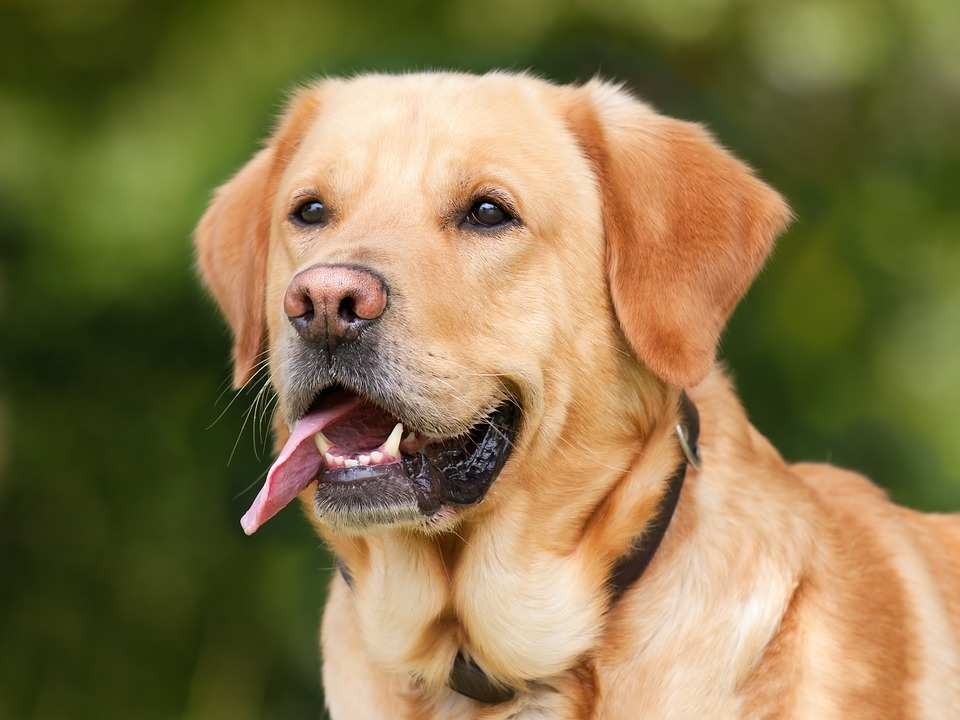
\includegraphics[height = 2.3cm]{images/weakness/Adi-003.png}}
    \hfill
  \subfloat[Pattern \cite{zhang_protecting_2018}\label{fig:trigger-c}]{%
       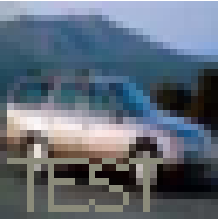
\includegraphics[height = 2.3cm]{images/protecting/Zhang-034.png}}
    \hfill
  \subfloat[Noise \cite{zhang_protecting_2018}\label{fig:trigger-d}]{%
        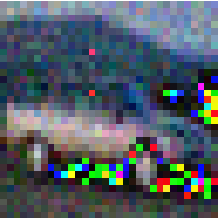
\includegraphics[height = 2.3cm]{images/protecting/Zhang-038.png}}
            \hfill
    \subfloat[Perturb. \cite{merrer_adversarial_2019}\label{fig:trigger-e}]{%
        
\includegraphics[height = 2.3cm]{images/frontier/merrer-011.png}}
        
    \caption{Examples for the various types of trigger images, intentionally labelled as a different class ((a), (b) as "cat", (c), (d) as "airplane", (e) as "9")}
    \label{fig:blackbox}
\end{figure*}
% -------------------------- %

Zhang et al. \cite{zhang_protecting_2018} propose the first black-box watermarking scheme in 2018 and introduce three types of trigger images: \textit{unrelated} (OOD), \textit{content} (pattern based) and \textit{noise} (based). %, as described above.
Their work forms the basis for many following papers.
%prime candidate for deletion. Can also be moved to an appendix where we gather some peculiar stuff. But I think it clearly fulfills our exclusion criterion.
%For the sake of completeness, we note that Zhang et al.'s work got re-implemented by Deeba et al. \cite{deeba_digital_2020}\footnote{Earlier version \cite{deeba_protecting_2019}} on another dataset. Their evaluation do not reveal any negative aspects of Zhang et al.'s work.

\subsection{Out-of-distribution}
Similar to and shortly after Zhang et al. \cite{zhang_protecting_2018}, Adi et al. \cite{adi_turning_2018} propose to include abstract images as trigger images in the training dataset. Those abstract images are completely unrelated to the main classification task% of the trained model
, thus it is highly unlikely that a model that has not seen this data point (i.e. one not watermarked) will label it as the designated class. %Furthermore, they proposed to combine the embedding with a \textit{commitment scheme} for more security.

% ---- Quan: Watermarking Deep Neural Networks in Image Processing
%TODO: how are the inputs generated? using something specific?
One of the first watermarking schemes for image processing models was proposed by Quan et al. \cite{quan_watermarking_2020}. The main difference to classification is that the output is, like the input, an image and not a label -- thus they are generating input-output pairs which consist of trigger images and verification images. They propose to use OOD images (or random noise) as trigger images and create the verification images by applying a simple image processing method to the trigger images (ideally not the one trained by the model). The idea is the same as in (defensive) backdooring. They generate input-output pairs where each consists of a trigger image and a verification image. The model is then fine-tuned on the union of the training dataset and the trigger set.
%The watermark verification is performed by querying the trigger image and comparing the output image with the verification image.

% ----- Yang: Effectiveness of Distillation Attack and Countermeasure on Neural Network Watermarking --- does not rely on specific choice of trigger images
Yang et al. \cite{yang_effectiveness_2019} empirically show that distillation is an effective watermark removal attack.
%Distillation is a type of compression where the knowledge of the original model (teacher model) is distilled into another smaller model (student model) \cite{hinton_distilling_2015}.
Therefore, they propose a new watermarking scheme, called \textit{ingrain}, that the authors claim to be especially robust against distillation. The main idea is that the watermark information is carried by the predictions of the original training data but the watermark extraction is done by querying trigger images that are drawn from a different distribution than the original images. Comparing to \cite{adi_turning_2018} and \cite{zhang_protecting_2018}, the target model is not trained on the union of the original training dataset and the trigger set, but only on the original dataset, and instead makes use of another model, the \textit{ingrainer model}, which influences the target model by a regulariser term to the loss function. The ingrainer model has the same architecture as the target model and is only trained on the trigger set, in particular, to overfit the trigger set.
%Roughly speaking, the model for the main classification task $\mathcal{F}_{\mathbf{w}}$ is influenced by another model, the ingrainer model $\mathcal{G}_{\mathbf{\theta}}$, which carries the watermark information, has the same architecture as the original model and is trained on the trigger set, in particular to overfit the trigger set.
% The ingrainer model stays fixed in the process of training the original model. The original model is then trained on both the original dataset and the trigger set. The influence of the ingrainer model is attained by adding a regulariser term to the loss function which is controlled by the ingrainer model $\mathcal{G}_{\theta}$.

\subsection{Pattern} \label{sec:black-box:pattern}
% ------ Li: Piracy Resistant Watermarks for DNNs
An improved pattern based technique was proposed by Li et al. \cite{li_piracy_2020}. They show that previous schemes \cite{adi_turning_2018, zhang_protecting_2018} are vulnerable to \textit{ownership piracy} attacks, in which an attacker aims to embed his own watermark into an already watermarked model. They propose a watermarking scheme that is especially robust against such attacks using \textit{dual embedding}: %, combining null embedding and true embedding.
the model is trained to classify (i) data with a pre-defined binary pattern correctly (\textit{null embedding}), and (ii) data with an inverted pattern (binary bits are switched) incorrectly (\textit{true embedding}). 
In more detail, for a pre-defined binary valued pattern $p$ and a very large number $\lambda$, the pattern $p$ is dual embedded into the model $\mathcal{F}_w$ if for all $X \in \mathbb{R}^n$ holds
\begin{align}
     \mathcal{F}_w(\mathrm{apply}(X, p, \lambda)) = \mathcal{F}_w(X) = y, \label{eq:nullembedding} \\ 
     \mathcal{F}_w(\mathrm{apply}(X, \mathrm{inv}(p), \lambda)) = \hat{y} \neq y, \label{eq:trueembedding}
\end{align}
where $\mathrm{apply}(X, p, \lambda)$ applies the pattern $p$ with magnitude $\lambda$ (value $\lambda$ for bit 1 and value $-\lambda$ for bit 0) to the image $X$. \cref{eq:nullembedding} refers to null embedding and \cref{eq:trueembedding} to true embedding.
%In null embedding the model is trained to classify the data with an embedded binary pattern correctly and in true embedding the model is trained in a way that images with an inverted pattern (binary bits are switched) are classified incorrectly.
% We define dual embedding: for a pre-defined binary valued pattern $p$ and a very large number $\lambda$, the pattern $p$ is dual embedded into the DNN model $\mathcal{F}_w$ if for all $X \in \mathbb{R}^n$ holds
% \begin{align}
%     \mathcal{F}_w(\mathrm{apply}(X, p, \lambda)) = \mathcal{F}_w(X) = y, \label{eq:nullembedding} \\ 
%     \mathcal{F}_w(\mathrm{apply}(X, \mathrm{inv}(p), \lambda)) = y_w \neq y, \label{eq:trueembedding}
% \end{align}
% where $\mathrm{apply}(X, p, \lambda)$ applies the pattern $p$ with magnitude $\lambda$ (value $\lambda$ for bit 1 and value $-\lambda$ for bit 0) to the image $X$. \cref{eq:nullembedding} refers to null embedding and \cref{eq:trueembedding} to true embedding. $\mathrm{inv}(p)$ denotes the inverted pattern, which means that the binary values in $p$ are switched. When the inverted pattern is applied, the model is trained to predict any other label $y_w$ than the original label.
They observe that null embedding does not degrade the model's accuracy if the number of pixels in the pattern is sufficiently small.
%and that "once a model is trained and null embedded, an adversary cannot null embed a pirate pattern without largely degrading the model's classification accuracy". 
% This scheme differs from other works because it uses large values $\lambda$ to generate the trigger image and therefore is more robust against backdoor detection like Neural Cleanse \cite{wang_neural_2019}.
Furthermore, they evaluate the robustness against model extraction attacks and conclude that, with enough (at least the same amount of) in-distribution data, the attacker is able to make a copy of the model without the watermark. For out-of-distribution data, the attacker would need 12.75 times more input data to reach similar accuracy.

% ---- Guo: Watermarking Deep Neural Networks for Embedded Systems
Guo et al. \cite{guo_watermarking_2018} propose to embed a pattern into the trigger images that can be clearly associated with the model owner's signature, e.g. a logo. The pattern should be embedded with little visibility so that the original model would still classify the trigger images to their original labels. The signature is used as a key to determine the pattern and then embedded in the image.% with an adjustable magnitude. 
%After embedding the watermark into the model, in other words after training the model with the original training set augmented by the trigger set, the watermarked model will be able to recognise images with the embedded pattern, and label them to a different class than the original one.
%The proposed way to create a unique pattern is the following: the model owner generates the $T$-bit signature by hashing a message and uses it as the key to a pseudorandom random permutation, which will define the location of the $T$ pixels, that will be changed. The 0/1-bits from the signature are transformed to -1/1 values and located on the defined pixels, which all together will form a pattern $p$ that will be added to the image $X$ with an adjustable magnitude $\alpha$.

% ---- Evolutionary trigger set generation --- pattern based
Guo et al. \cite{guo_evolutionary_2019} propose an evolutionary algorithm-based method to generate and position trigger patterns, based on \cite{zhang_protecting_2018} and \cite{guo_watermarking_2018}. %This should lead to a significant reduction in false positive rates of the watermarked model.
Their algorithm is based on Differential Evolution \cite{storn_differential_1997}, %TODO: remove reference if we need reference space
an evolutionary algorithm and a metaheuristic that searches for the optimal solution for an optimisation problem.
%TODO: describe what is the optimisation - position for log embedding? what for noise?
Using this trigger pattern generation they demonstrated an improvement in integrity and robustness.
% Nur für mich, als Info. Bin mir noch nicht sicher, ob ich das erwähne:
% It is worth noting that "Guo et al. found that embedding a new watermark using limited amount of data would degrade the model's performance. Therefore, they ruled out this possibility of attack."

\subsection{Noise}
% ---- Secure NN WM protocol --- noise?
Zhu et al. \cite{zhu_secure_2020} propose a watermarking scheme especially to defend against watermark overwriting (forging attacks). They propose to use one-way hash functions for both generating the trigger image and label.
%trigger image generation. Let $H_X$ be a hash function that takes an image and a key as input and outputs an image and $H_y$ a hash function that takes an image as input and outputs an integer value. $H_X$ is used to generate the trigger images and $H_y$ to generate the corresponding labels.
The framework takes an initial image and creates a hash chain of trigger images, as shown in \cref{fig:zhu}. They show experimentally that their proposed scheme is robust against forging attack even if the attacker knows the trigger set generation algorithm.
%protocol for trigger generation.

\begin{figure}[t]
    \centering
    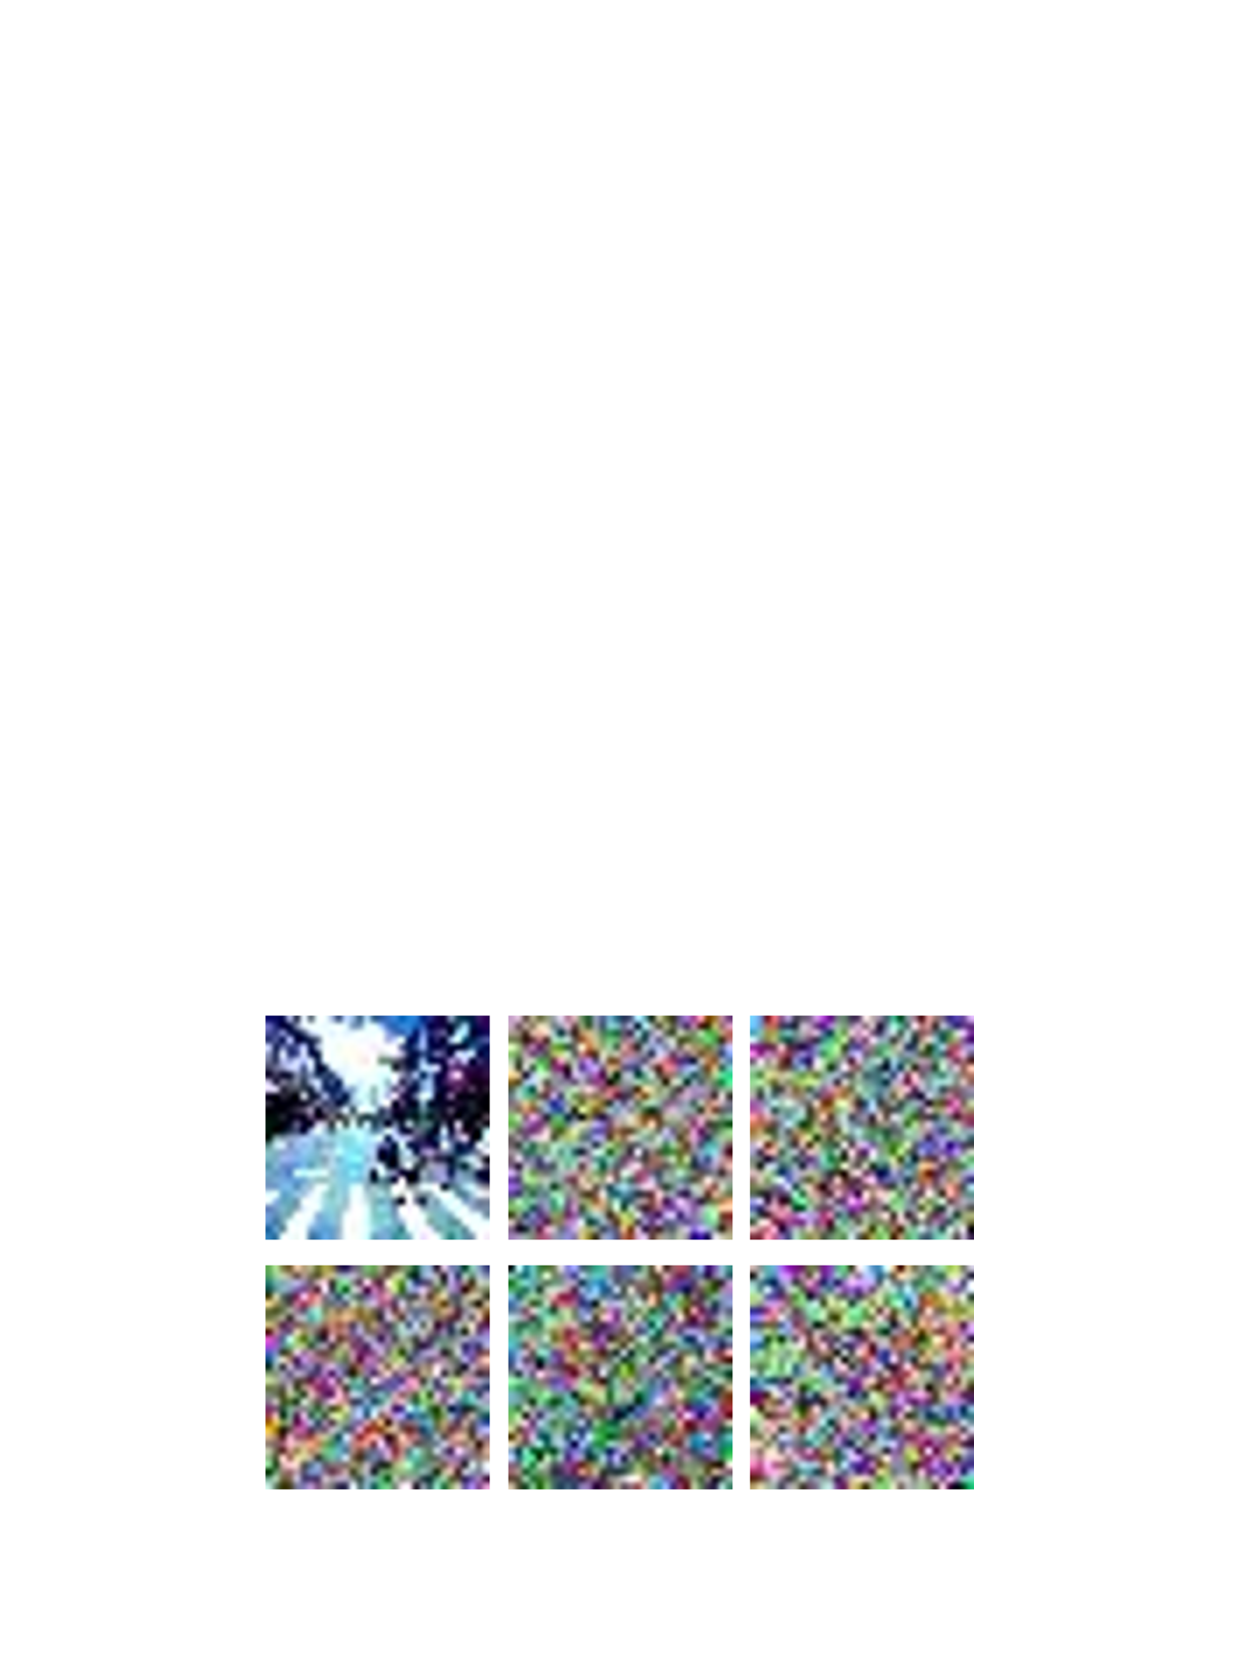
\includegraphics[width = 0.4 \textwidth]{images/Zhu1.pdf}
    \caption{The upper left image is the initial image and the following five are trigger images resulting from a hash chain \cite{zhu_secure_2020}.}
    \label{fig:zhu}
\end{figure}

\subsection{Perturbation}
% ---- adversarial frontier stitching
Another black-box scheme was proposed by Merrer et al. \cite{merrer_adversarial_2019}. The goal is to slightly shift the decision boundary of the model. This is achieved by generating adversarial examples \cite{szegedy_intriguing_2014} for images close to the boundary, and changing the class for those adversaries. % to the neighbouring class.
After fine-tuning the model, the decision boundary is adapted. An illustration of this decision boundary shifting for a two class boundary is given in \cref{fig:merrer}.

\begin{figure}[t]
    \centering
    \hspace*{\fill}
  \subfloat[\label{fig:merrer-a}]{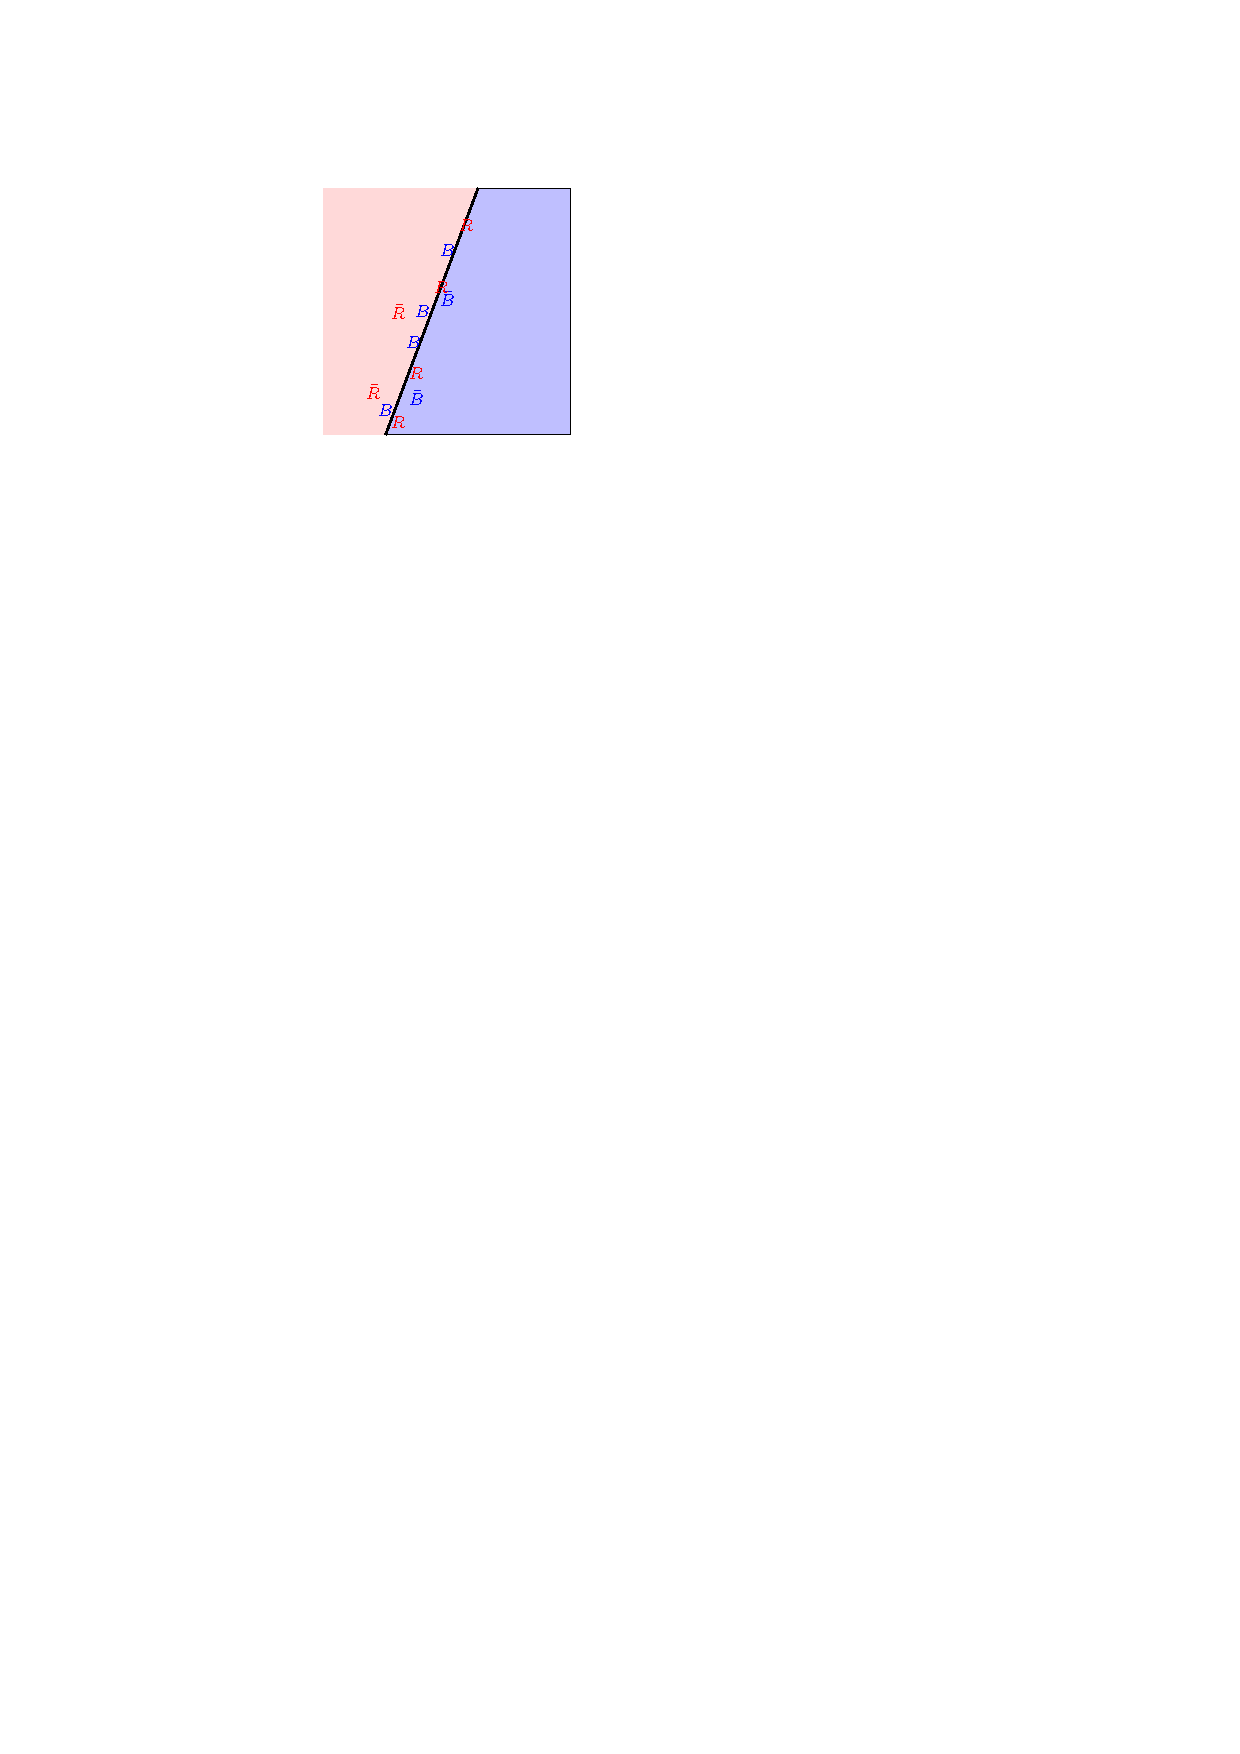
\includegraphics[width = 0.2 \textwidth]{images/frontier/Merrer1.pdf}}
    \quad
  \subfloat[\label{fig:merrer-b}]{
\includegraphics[width = 0.2 \textwidth]{images/frontier/Merrer2.pdf}}
    \hspace*{\fill}
    \caption{(a) The data points are divided into "true adversaries" ($R$ and $B$) and "false adversaries" ($\bar{R}$ and $\bar{B}$). The label for the true adversaries is changed, the label for the false adversaries stays unchanged. (b) After fine-tuning the decision boundary changes. \cite{merrer_adversarial_2019}}
    \label{fig:merrer}
\end{figure}

% ----- GAN-based technique
Li et al. \cite{li_how_2019} especially address evasion attacks. They propose a framework closely related to the idea of GANs. They use three DNNs: encoder, discriminator, and target model. The encoder takes the original image and aims to embed a logo into the image such that the difference is imperceptible. The resulting trigger images are fed into the discriminator together with the original image to evaluate the encoder's success.
%detect if the trigger image was generated by the encoder. 
%The networks are trained iteratively until they reach their optimum.
%Finally, the target model is trained with the original images together with the generated trigger images.
A difference in the original and trigger images is essential for the watermarking scheme, yet the goal is to make the difference as small as possible. This framework especially deals with the trade-off between security and effectiveness. The smaller the difference, the better security against evasion attacks, and the larger, the better the effectiveness of the embedded watermark.

% ---- Chen: BlackMarks - nicht sicher ob ich zu perturbation zuordnen kann
Chen et al. \cite{chen_blackmarks_2019} propose the watermarking framework \textit{BlackMarks}, which %embeds a binary signature into a model and can be verified in the black-box setting.
encodes the signature within the distribution of the output activations. % (before applying softmax). %, and creates targeted adversarial attacks as trigger images.% and labels.
To encode the class predictions, the authors design a scheme that maps the class predictions to binary bits, by clustering the original classes into two categories, represented by bit 0 and bit 1. The trigger images are created in a way that for the bit 0, an adversarial example that would belong to the cluster represented by the bit 1 is created, and is labelled with a uniformly randomly chosen class from the cluster represented by the bit 0. Trigger images for the bit 1 are created vice-versa. The watermark is extracted by querying the trigger images and encoding each class to a binary value, which should result in the owner's binary signature to prove ownership.

\subsection{In-distribution}
Namba et al. \cite{namba_robust_2019} propose an attack, called \textit{query modification}, that investigates the query for trigger images in order to invalidate the watermark (cf. \cref{sec:attacks}). With that in mind, they propose a scheme that is more robust especially against query modification but also model modifications like fine-tuning and model compression (e.g. pruning). The query modification as an attack exploits the fact that trigger images differ from original training images. Therefore, they propose to use trigger images that are selected from the training sample distribution.
%They randomly select a sample of images from the training data and change the label, e.g. from "dog" to "cat". After embedding, the model will classify, for instance, all dog images correctly but only this specific one as "cat".
The trigger images are thus undetectable, however, the model is more likely to overfit to the (on purpose) wrongly labelled triggers, and thus more susceptible to removal attacks via e.g. pruning. They want to counter pruning by ensuring that the predictions do not depend on a large number of small model parameters that would likely be pruned. Thus, the model is first trained as usual with the original training set. Then, the watermark is embedded by exponentially weighting the parameters and training the model on the union of the training dataset and the trigger set, which enforces the predictions to depend on a small number of large parameters instead.
In exponential weighting the model parameters $\mathbf{w}^l$ are changed in every layer $l$ by
\begin{align} \label{eq:exponential-weighting}
     \mathbf{w}_{\mathrm{exp},i}^l = \frac{\lambda \mathrm{exp}\, |\mathbf{w}_i^l|}{\mathrm{max}_i \, \lambda \mathrm{exp} \, |\mathbf{w}_i^l|}\mathbf{w}_i^l,
\end{align} %in original paper: theta statt w und T statt lambda
where $\mathbf{w}_i^l$ denotes the $i$-th component of the parameter vector $\mathbf{w}^l$ in layer $l$ and $\lambda$ is an adjustable parameter for the intensity of the weighting.

\subsection{Trigger labelling}
% ----- Zhong: Protecting IP of Deep Neural Networks with Watermarking: A New Label Helps --- does not rely on specific choice of pattern
Zhong et al. \cite{lauw_protecting_2020} propose to label the trigger images with a completely new label, rather than assigning one from the existing labels, so that the watermark embedding has only little impact on the original classification boundaries.
Any pattern based trigger image can be used in this context. They compare their work to \cite{zhang_protecting_2018} in their experimental evaluation and show that the proposed scheme achieves a zero false-positive rate, i.e. excellent integrity, and is more robust against fine-tuning and model compression.

Zhang et al. \cite{zhang_deeptrigger_2020} observe that frequently, trigger images are created in a systematic way, and it is thus easier for an attacker to re-create them.
Therefore, they propose to include unpredictability in the labels assigned to the trigger images. They use a chaos-based labelling scheme for trigger images that ensures that an attacker cannot produce a valid trigger set, even if he knows the trigger pattern.

% ----- Xu: Identity Bracelets --- does not rely on specific choice of trigger images
Xu et al. \cite{xu_identity_2020}\footnote{Previous pre-print version in \cite{xu_novel_2019}} propose, similar to \textit{BlackMarks} \cite{chen_blackmarks_2019}, a watermarking scheme that carries the watermark information within the output activations. The trigger pairs consist of a trigger image and a serial number (SN) which is constructed individually by the owner's rules. The SN is composed by using the probabilities in the last layer.
%For instance, for the MNIST dataset, which has 10 different classes, the SN could be a 10 digit number but also a 20 digit number by adding zeros to the classical 10 dimensional one-hot encoding. In particular, if the generated SN is "558831271817-2355-7965", the digits must be reduced by two orders of magnitude and added 0.001. The resulting probabilities that should be predicted by the given trigger images are [0.051, 0.051, 0.081, 0.081, 0.031, 0.011, 0.021, 0.071, 0.011, 0.081, 0.011, 0.071, 0.021, 0.031, 0.051, 0.051, 0.071, 0.091, 0.061, 0.051].
It is worth noting that any rule for generating it is feasible. For instance, for three classes the SN could be "235" following the rule to reduce the digits by one order, resulting in [0.2, 0.3, 0.5], but also any other, more complex rule can be used. The proposed scheme does not rely on the specific choice of trigger images since it focuses on the output activations. 

\subsection{Countering Model Extraction} \label{sec:wm:countering_extraction}
% --- Jia: EWE
Only a few schemes address the second threat model case in \cref{sec:threatmodel}, i.e. robustness against model extraction attacks. %, we have to consider other watermarking frameworks than the ones introduced before.
Jia et al. \cite{jia_entangled_2020} are the first to propose a scheme, called \textit{entangled watermark embedding} (EWE). %, which they claim and evaluate to be robust against tested model extraction techniques.
%They observe that watermarks are usually outliers in the distribution of the training data and that watermarked models can be separated into two sub-models, one for the main task and the other one for watermarking. The latter one usually does not survive model extraction.
The main idea is to create a watermarked model that is not specialised into "sub-models", where one part of the model is capable of the main classification task, and the other for watermark detection (which normally is lost during the model extraction attack). This is achieved by a regulariser term ensuring that the trigger images lead to similar activation patterns as the original images. Thus, both trigger images and original images cause a similar behaviour of the model, thereby increasing the robustness against model extraction.  
% They make use of the soft nearest neighbour loss (SNNL) \cite{kornblith_similarity_2019, salakhutdinov_learning_2007}. %TODO: if space is needed in references, remove one of those two
%"which measures the distance between points from different groups relative to the average distance for points within the same group."
%Data points are forming clusters when the SNNL is minimised and they are entangled when the SNNL is maximised.
%In EWE, the trigger images generation works as follows: two similar classes are chosen. If the images from the classes are similar, it will be easier to entangle them. 
%The trigger pattern is chosen and the location for the pattern is determined where the gradient of the SNNL is largest. During embedding, the negative SNNL is used as a regulariser term in the fine-tuning process. In this way, the watermarks and original data points are entangled and more robust against extraction attacks.
% TODO: could mention that they also test their scheme for audio classification

% ---- Szyller: DAWN
%Another defence against model extraction was proposed by 
Szyller et al. \cite{szyller_dawn_2020} propose the framework \textit{Dynamic Adversarial Watermarking of Neural Networks} (DAWN), which is not embedding a signature into the target model itself but dynamically returning wrong classes from the API service for a fraction of queries to mark an adversary model created via a model extraction attack.
It is worth noting that the scheme is not able to differentiate between an attacker and a benign client -- all clients obtain a fraction of wrong predictions. %Whether a specific response should be watermarked, and which wrong class to use for the watermark, is based on a hash function.
%keyed cryptographic hash function as a source for randomness.
It is ensured that the same query always returns the same output (correct or modified). Whenever a wrong prediction is returned, the input-output pair is saved so that in need of a watermark verification, they can be used for triggering the stolen model. This approach thus realises \circled{4} in \cref{fig:watermarking-ml-process}.

% ---- Zhang: Model Watermarking for Image Processing Networks
Zhang et al. \cite{zhang_model_2020} and Wu et al. \cite{wu_watermarking_2020} propose, independently of each other, a similar approach to \cite{szyller_dawn_2020}, as they are hiding an invisible watermark in the outputs of the image processing model, but for \textit{all} outputs. When an attacker trains a new (surrogate) model on the input-output pairs of the original model, the watermark will be learned too and can be verified with black-box access (cf. \circled{4} in \cref{fig:watermarking-ml-process}). The major difference to \cite{szyller_dawn_2020} is that in the case of an image processing model, the output is another image, and thus there is more data to embed the watermark in. Both papers are not explicitly addressing model extraction attacks, but we believe they are a suitable defence.
%Wu et al. train a target network, which learns to embed the watermark, and a watermark extraction network, which learns to extract the watermark, together by optimising a combined loss function.

% % ------ Wu: Watermarking Neural Networks with Watermarked Images
% is similar to Zhang above. Unified those two.
% Wu et al. \cite{wu_watermarking_2020} proposed a black-box model watermarking framework for image processing models that watermarks every ouput of the model, like \cite{zhang_model_2020}. They train a target network, which learns to embed the watermark, and a watermark extraction network, which learns to extract the watermark, together by optimising a combined loss function.

\subsection{Watermarking for specific ML settings}
% % ---- Sakazawa: Visual Decoding of Hidden Watermark in Trained Deep Neural Network
% In contrast to other work, which mainly focuses on watermark embedding, Sakazawa et al. \cite{sakazawa_visual_2019} focuses on the watermark extraction. They propose a "cumulative and visual decoding" of watermarks in deep neural networks and experimentally show that their proposed method can successfully decode simple watermarks from trigger images.
% % nicht in requirements tabelle weil keine embedding methode

%---> paper sieht sehr mies aus.

% ------ Atli: WAFFLE: Watermarking in Federated Learning
% "framework"
Existing watermarking schemes are not suitable for Federated Learning (FL), as pointed out by Atli et al. \cite{atli_waffle_2020}. Embedding a watermark in such a setting is different, because the model owner has no access to training data, and the training is performed in parallel by several clients.
%Therefore, the model owner cannot embed the watermark on the training data and neither the clients because one of them could be malicious.
Atli et al. %developed a black-box watermarking scheme for client-server FL via backdooring. They 
propose to include an independent and trusted party between the model owner and the clients. The independent party has the ability to embed a black-box watermark based on backdoors into the model at every aggregation step.
%Could be deleted, not essential. But maybe moved to noise pattern section?
Furthermore, they propose a watermarking pattern that is a specific noise pattern.
% Ist nicht in den requirements tables enthalten. Weil nicht vergleichbar mit den anderen. Listet ähnliche aber dennoch sehr spezifische requirements auf.

% ------ Skripniuk: Black-Box Watermarking for Generative Adversarial Networks
Skripniuk et al. \cite{skripniuk_black-box_2020} propose the first, and until now only, watermarking scheme specially crafted for GANs. The existing watermarking schemes are limited to DNNs that map from images to classes, and thus could not be transferred to GANs. The authors watermark the input images and then transfer the watermarked images to the GAN model. First, the image steganography system has to be trained, which consists of an encoder and decoder,
%The encoder takes an image and an watermark and produces a watermarked image, whereas the decoder takes the watermarked image and outputs the embedded watermark.
and subsequently, \textit{all} the training data together with a secret watermark is fed to the encoder resulting in watermarked data. The watermarked data is then used to train the GAN model. For verification, the model owner only needs an output image of the GAN, and applies the decoder on it to compare the result with the secret watermark. Thus, the proposed scheme needs only black-box access for verification.

% ------ Lim: Protect, Show, Attend and Tell: Empower Image Captioning Model with Ownership Protection
Lim et al. \cite{lim_protect_2020} are the first to propose watermarking for a recurrent neural network (RNN). Specifically, they consider an image captioning model, implemented as a simplified variant of the \textit{Show, Attend and Tell} model \cite{xu_show_2015}, where the output of the model is a sequence (the caption). The proposed framework is similar to \cite{fan_rethinking_2019}, but does not embed the verification information (the owner's key) into the model weights, but into the signs of the hidden states of the RNN.
During model inference time, the key is required as input to the model by an element-wise combination with the input data.
Without the correct key provided, the effectiveness of the model drops significantly.

\section{Fingerprinting of ML Models} \label{sec:fingerprinting}

Imagine a software company is selling their ML model to different customers, but the model got illegally redistributed by one of them. The company would like to gather evidence on the leak and therefore could embed fingerprints in the ML model before selling the product, in order to trace back the user when needed. We can think of fingerprinting as an extension of watermarking on a user level.
%
At the time of performing this survey, fingerprinting for ML models was not extensively discussed, with only three papers %on this topic were 
published.

Note that there is another notion of fingerprinting. In cyber security, a (unique) identifier for an object (either hardware, software, or a combination thereof) is generally referred to as a fingerprint, e.g. such as in browser fingerprinting~\cite{eckersley_how_2010} or device fingerprinting~\cite{kohno_remote_2005}. The application scenario for employing these techniques is often in tracking devices (resp. their users). Because this context differs from what we considered so far, we call this form \textit{Fingerprinting as unique identification}.

\subsection{Fingerprinting as User-specific Watermark}
\label{sec:fingerprinting:user-specific-wm}
%The owner wants to distribute a model to multiple users, each having an individual fingerprint embedded in the model, to verify the malicious user in case of ownership infringement.

% regulariser based
Chen et al. \cite{chen_deepmarks_2019} propose a white-box fingerprinting framework, \textit{DeepMarks}, that is able to embed unique fingerprints. The verification process not only detects the attacker, but detects also if multiple, and if so which, users collaborated in order to create an unmarked model. The embedding process works similar to the one in \cite{rouhani_deepsigns_2019}. They propose to assign a unique binary vector (fingerprint) to each user and embed the fingerprint information in the PDF of the weights before distributing the models to the users.

Although \textit{DeepMarks} is the only paper considering especially fingerprinting, we believe that a couple of the above introduced watermarking schemes can be extended to fingerprinting. To name a few, \cite{uchida_embedding_2017} embeds a unique signature into the weights of the DNN, \cite{li_how_2019} embeds a unique logo into the trigger images and \cite{guo_watermarking_2018} generates unique trigger images based on a signature. All of them could embed user-specific watermarks. Moreover, \cite{xu_identity_2020} relies on serial numbers that can be created in indefinitely many ways, assigning each to a user.

\subsection{Fingerprinting as Unique Model Identifier}
%However, a unique identification of a ML model is not secure enough for our threat model. For example, 
Cao et al. \cite{cao_ipguard_2020} propose a framework to obtain a unique identifier of DNNs. %by "fingerprinting" the classification boundary of DNNs.
Based on the idea that two different models have different classification boundaries, they propose to "fingerprint" the classification boundary of the model. If the model was changed in the slightest way, the classification boundary would slightly shift too. This scheme, however, does not fit our threat model, as we want to recognise the original model even after (especially minute) model modifications. We, therefore, require a fingerprinting framework to be more robust to model modifications.

% also fan_rethinking_2019 mentions a "signature" of signs in some layers as fingerprint / signature string

% perturbation
% man könnte diesen Absatz natürlich auch zu perturbation based geben. Der Unterschied ist, zB zu Merrer (der extra trigger images nahe zur classification boundary generiert und dann damit fine-tuned um die classification boundary etwas zu shiften), dass sie die adversarial images finden, aber dann in das model einbetten.
Zhao et al. \cite{zhao_afa_2019} and Lukas et al. \cite{lukas_deep_2020} modify this idea of fingerprinting as unique identification. Both propose a scheme in which the adversary model, created by applying modifications to the target model, has the same fingerprint as the target model. They both introduce a novel algorithm for creating transferable adversarial examples \cite{liu_delving_2017}. %These adversarial examples are slightly different from the original image but different enough to fool the model to classify the image incorrectly.

Note that in \cref{sec:blackbox} we describe how black-box watermarking methods use perturbation based trigger images (adversarial examples), which are used during training so that the models learn how to (purposefully) misclassify them.
In the context of fingerprinting as a unique model identifier, the authors want to create an adversarial example from an already trained ML model. The key aspect is that the generated images are not only adversarial examples for the target model, but also for the adversary model, i.e. they are transferable to the adversary model. This %, in contrary to Cao et al.'s work \cite{cao_ipguard_2020}, 
fits our first threat model case in \cref{sec:threatmodel}.

\section{Attacks on Watermarking Methods}
\label{sec:attacks}

If the attacker knows or suspects that a model is protected, he could try to change the model in order to remove or overwrite the protection. 
Regarding watermarking, most authors claim that their techniques are robust against various model modifications like \textit{fine-tuning}: re-training the model with new data and \textit{parameter pruning}: setting small parameter values to zero, which is a model compression technique \cite{han_deep_2016,zhu_prune_2017}. %molchanov_pruning_2017, li_pruning_2017,
But further attacks were proposed that are aiming to remove, overwrite, detect or invalidate state-of-the-art watermarking schemes, which we will analyse. % We dedicate this section to those works. 
We want to point out that most of the techniques, except of \textit{EWE} \cite{jia_entangled_2020} and \textit{DAWN} \cite{szyller_dawn_2020}, are not robust against model extraction (model stealing) attacks \cite{tramer_stealing_2016}, as pointed out by Mosafi et al. \cite{mosafi_stealing_2019}.

%cell color: \cellcolor[HTML]{ECECEC}

%\begin{table*}[t]
\begin{sidewaystable}
\caption{Which attack defeats which watermarking technique based on the evaluation of the papers. A $\sim$ denotes that the authors claim that their attack can be extended easily to defeat this watermarking technique but did not provide an evaluation for that.} 

\centering
\resizebox{\textwidth}{!}{\begin{tabular}{lll|l|l|l|l|l|l|}
\cline{4-9}
                                                              &                                                            &              &  \multicolumn{6}{l|}{Watermarking techniques}                                                                     \\ \cline{4-9} 
                                                              &                                                            &              & OOD & pattern      & noise       & perturbation & in-distribution & regulariser   based          \\ \hline
 \multicolumn{1}{|l|}{\multirow{12}{*}{\rotatebox[origin=c]{90}{Attacks on watermarks}}} & \multicolumn{1}{l|}{\multirow{2}{*}{invalidation}}         & Hitaj et al. \cite{hitaj_evasion_2019}        & \cite{adi_turning_2018},   \cite{zhang_protecting_2018}$\sim$      &              &             & \cite{merrer_adversarial_2019}$\sim$     &                 &                              \\ \cline{3-9} 
\multicolumn{1}{|l|}{}                                        & \multicolumn{1}{l|}{}                                      & Namba et al. \cite{namba_robust_2019}        & \cite{zhang_protecting_2018}               & \cite{zhang_protecting_2018}        & \cite{zhang_protecting_2018}       & \cite{merrer_adversarial_2019}       &                 & \cite{rouhani_deepsigns_2019}                      \\ \cline{2-9} 
\multicolumn{1}{|l|}{}                                        & \multicolumn{1}{l|}{overwriting}                           & Li et al. \cite{li_piracy_2020}           & \cite{adi_turning_2018}, \cite{zhang_protecting_2018}                 & \cite{zhang_protecting_2018}        & \cite{zhang_protecting_2018}        &              &                 &                              \\ \cline{2-9} 
\multicolumn{1}{|l|}{}                                        & \multicolumn{1}{l|}{detection}                                      & Wang et al. \cite{wang_robust_2020}  &                     &              &             &              &                 & \cite{uchida_embedding_2017},   \cite{rouhani_deepsigns_2019}            \\ \cline{2-9} 
\multicolumn{1}{|l|}{}                                        & \multicolumn{1}{l|}{\multirow{3}{*}{detection,   removal}} & Wang et al. \cite{wang_attacks_2019} &                     &              &             &              &                 & \cite{uchida_embedding_2017}                       \\ \cline{3-9} 
\multicolumn{1}{|l|}{}                                        & \multicolumn{1}{l|}{}                                      & Shafieinejad et al. \cite{shafieinejad_robustness_2019} & \cite{adi_turning_2018},   \cite{zhang_protecting_2018}        & \cite{guo_watermarking_2018},   \cite{zhang_protecting_2018} & \cite{zhang_protecting_2018} &              &                 &                              \\ \cline{2-9} 
\multicolumn{1}{|l|}{}                                        & \multicolumn{1}{l|}{\multirow{5}{*}{removal}}              & Liu et al. \cite{liu_removing_2020}          & \cite{adi_turning_2018},   \cite{zhang_protecting_2018}        & \cite{guo_watermarking_2018},   \cite{zhang_protecting_2018} & \cite{zhang_protecting_2018}       &              &                 &                              \\ \cline{3-9} 
\multicolumn{1}{|l|}{}                                        & \multicolumn{1}{l|}{}                                      & Aiken et al. \cite{aiken_neural_2020}        & \cite{adi_turning_2018},   \cite{zhang_protecting_2018}        & \cite{zhang_protecting_2018}        & \cite{zhang_protecting_2018}       &              &                 &                              \\ \cline{3-9} 
\multicolumn{1}{|l|}{}                                        & \multicolumn{1}{l|}{}                                      & Guo et al. \cite{guo_hidden_2020}          & \cite{adi_turning_2018}                 & \cite{zhang_protecting_2018}        &             & \cite{merrer_adversarial_2019}       &                 &                              \\ \cline{3-9} 
\multicolumn{1}{|l|}{}                                        & \multicolumn{1}{l|}{}                                      & Chen et al. \cite{chen_refit_2020}        & \cite{adi_turning_2018},   \cite{zhang_protecting_2018}        & \cite{zhang_protecting_2018}        &             & \cite{merrer_adversarial_2019}       & \cite{namba_robust_2019}           &                              \\ \cline{3-9} 
\multicolumn{1}{|l|}{}                                        & \multicolumn{1}{l|}{}                                      & Yang et al. \cite{yang_effectiveness_2019}         &                     &              &             &              &                 & \cite{uchida_embedding_2017},   \cite{rouhani_deepsigns_2019}, \cite{chen_deepmarks_2019} \\ \hline
\end{tabular}
}
\label{tab:attacks}
\end{sidewaystable}
%\end{table*}


% \cite{hitaj_evasion_2019}
% \cite{namba_robust_2019}
% \cite{li_piracy_2020}
% \cite{sakazawa_visual_2019}
% \cite{wang_attacks_2019}
% \cite{wang_robust_2020}
% \cite{shafieinejad_robustness_2019}
% \cite{liu_removing_2020}
% \cite{aiken_neural_2020}
% \cite{guo_hidden_2020}
% \cite{chen_refit_2020}
% \cite{yang_effectiveness_2019}

% \cite{adi_turning_2018}
% \cite{zhang_protecting_2018}
% \cite{merrer_adversarial_2019}
% \cite{guo_watermarking_2018}
% \cite{namba_robust_2019}
% \cite{rouhani_deepsigns_2019}
% \cite{uchida_embedding_2017}
% \cite{chen_deepmarks_2019} 
In \cref{tab:attacks}, we summarise the attacks on watermarking schemes.
%, which are going to be discussed in the section.
Each line corresponds to an attack and each column to a (type of) watermarking scheme. The table shows which attack defeats which kind of watermarking. We list only schemes that were proven to be successfully defeated -- missing schemes in the table do not imply strong robustness. We can see that an attack usually addresses either white-box or black-box watermarking schemes. The four trigger image types OOD, pattern, noise and perturbation based seem to be defeated in a similar way. In-distribution watermarks are more difficult to detect or remove, probably because of the fact that they do not differ from the original training data distribution.
%We are going to present the works divided into four types of attacks, which we introduced in \cref{sec:attack-model}: watermark overwriting, detection, removal, and invalidation.
 
\subsection{Watermark Overwriting}
Li et al. \cite{li_piracy_2020} show %, as a motivation for a novel watermarking scheme, 
that previous schemes \cite{adi_turning_2018, zhang_protecting_2018} are vulnerable to watermark overwriting (ownership piracy attack).
%In particular, they show it for \cite{adi_turning_2018} and \cite{zhang_protecting_2018}, pointing out that Wang et al. \cite{wang_attacks_2019} cover already regulariser-based schemes.
They %re-implemented the schemes from the original papers for 
apply the schemes to
four image classification tasks, %: digit recognition (MNIST), face recognition (YouTube Face), traffic sign recognition (GTSRB), and object recognition (CIFAR-10) 
and assume that an attacker would have access to around 10\% of the %5,000
original training images. Experimentally, the authors conclude that an attacker could successfully embed the pirate watermark by training the model with training data that is adapted to the pirate watermark.
  
\subsection{Watermark Detection}
Most black-box watermarking methods are based on backdoors. Therefore, backdoor detection algorithms like Neural Cleanse \cite{wang_neural_2019} and Fine-Pruning \cite{liu_fine-pruning_2018} could be a potential threat to these methods. Wang et al. \cite{wang_robust_2020} show that regulariser based watermarking schemes are vulnerable to watermark detection by the use of a property inference attack \cite{ganju_property_2018}.
Knowing the embedding algorithm, they train a set of shadow models (i.e. models with similar architecture and similar data), some of which will be watermarked, and some not.
From these models, they extract weights as representative features, and subsequently, train a model on these features to distinguish between watermarked and not-watermarked models.

\subsection{Watermark Removal}

Some of the attacks exploit the fact that a watermarked model actually learns two tasks: the main classification task and the watermarking task. This fact can be also observed in the increase of the model parameters' variance during watermark embedding \cite{wang_attacks_2019}.

% ---- Wang: Attacks on Digital Watermarks for Deep Neural Networks - detection and removal -- the variance of the distribution of model parameters
Wang et al. \cite{wang_attacks_2019} are one of the first to reveal serious vulnerabilities in watermarking schemes, in particular watermark detection and removal. They observe that in regulariser based watermarking methods like \cite{uchida_embedding_2017}, the variance of the distribution of model parameters, they call this \textit{weights variance} or \textit{weights standard deviation}, increases during watermark embedding.
%Their detection algorithm measured the variance of model parameters distribution, which they call \textit{weights variance}.
The watermark is removed by embedding one or several additional watermarks into the model, following the embedding scheme in \cite{uchida_embedding_2017}. Since every additional watermark might increase the weights variance, they propose to lower the weights variance by adding a $L_2$ regulariser. Following this procedure, the authors show that the old watermark cannot be extracted, thus the model owner cannot claim ownership anymore. It shall be noted that although additional watermarks are placed into the watermarked model, the main objective is to "neutralise" the old watermark rather than to use the new watermarks to claim ownership.

%In this way, the old watermark can be removed but also the attacker's own watermark can be placed.

% ----- Shafieinejad: On the Robustness of the Backdoor-based Watermarking in Deep Neural Networks -----
Shafieinejad et al. \cite{shafieinejad_robustness_2019} analyse the robustness of backdoor based watermarking schemes. In particular, they propose a model extraction (stealing) attack that trains a substitute model (cf. e.g. \cite{papernot_practical_2017}).
This is performed by querying the original model with a public dataset from the same domain and using the resulting label to train their own model. As the public dataset contains none of the trigger images, the watermark is "lost" in the process.
%steals the functionality of the target model and removes the embedded watermark without having any access to the model's parameters. %Similar to other attacks above, it exploits the fact that the watermarked model actually learns two tasks: the main classification task and the watermarking task, so that trigger images are seen as outliers for the main classification.
%TODO: they also adapt this to a white-box attack
Furthermore, similar to Wang et al. \cite{wang_robust_2020}, they propose to use property inference for watermark detection.
% TODO: haben die auch ein watermarking scheme? ein anderes paper behauptet das -> hätt ich jetzt nicht gefunden...

% ----- Liu: Removing Backdoor-based WM in Neural Networks with Limited Data -----
Liu et al. \cite{liu_removing_2020} propose \textit{WILD}, a framework against backdoor-based watermark techniques based on fine-tuning.
They argue that it is hard for adversaries to collect a large amount of unlabelled data within the same domain as the original training data, as required by \cite{shafieinejad_robustness_2019}, and that using non-domain data impacts the effectiveness of the substitute model.
Their special contribution is that only a small portion of training data is needed. They utilise Random Erasing \cite{zhong_random_2020}, i.e. removing random segments from the input images, to augment the data. %(quote: "to fine-tune the watermarked model robust against occlusion.")
This augmented data alone is, however, not enough to remove a watermark via fine-tuning, because of the high diversity of potential watermarks. They note that backdoor patterns are mostly learned by the high-level feature spaces produced by the convolutional layers, and not by the fully connected layers.
%, especially when only considering the fully-connected layers.
%Therefore, they proposed to consider a high-level feature space and hope
%They further consider fine-tuning once again by considering a high-level feature space. "The intuition behind is that the injected watermarks in neural networks form strongly correlated paths from the input layer to the output layer of the model. We can mitigate the impact of watermarks by weakening the effectiveness of these paths to make the benign object back in control. A good start point that sees all these special kernels is in the high-level feature space just after the final convolutional layer."
%that similarity between data with watermark pattern and clean data implies similarity in the distribution of high-level features of these data points. They %formulated an optimisation problem to minimise the distribution distance between them, and
%\begin{align*}
%\mathrm{minimize}\quad  &d(\mathcal{G}(x_{clean}), \mathcal{G}(x)),\\
%\mathrm{such \; that}\quad  &x \in \mathrm{apply}(x_{clean}, p, l),
%\end{align*}
%where $\mathrm{apply}(x,p,l)$ denotes applying watermark trigger pattern $p$ at location $l$ on data point $x$, and $d$ is a metric function measuring the distance between the two distributions in high-level feature space, i.e. $\mathcal{G}(x_{clean})$ and $\mathcal{G}(x)$.
%To minimise the distribution distance, they penalised the distribution distance during the process of fine-tuning by adding a penalty term to the loss function. 
%They 
%fine-tune the model using the augmented data, while adding a penalty term to minimise the distribution distance.
%The loss function $\mathcal{L}$ for their framework looks as follows:
% \begin{align*}
% \mathcal{L} = \mathcal{L}_{aug} + \beta \cdot d(\mathcal{G}(x_{clean}), \mathcal{G}(x_{aug})),
% \end{align*}
% where $\mathcal{L}_{aug}$ is the calculated loss when fine-tuning with the augmented data $x_{aug}$ and $\beta$ is the penalty coefficient that regulates the strength of the penalty item.
They therefore utilise the augmented data to fine-tune the model and add a regulariser (penalty) term that ensures a minimal distance in distribution between the high-level feature space of the augmented and the clean dataset, so that a backdoor pattern would not be learned.
The authors reveal that it is more difficult to remove OOD, compared to pattern based and noise based watermarks.

% The authors test WILD
% %on MNIST and CIFAR-10 datasets and 
% on three kinds of black-box trigger images: out-of-distribution, pattern based and noise based. In comparison, it is more difficult to remove the out-of-distribution watermark than the other ones. They claim that the main reason is that the poisonous data that is use in that case comes from totally different distributions.

% ----- Guo: The Hidden Vulnerability of Watermarking for Deep Neural Networks -----
Guo et al.'s removal attack \cite{guo_hidden_2020} % does neither require knowledge of the embedding technique nor labelled samples. The attack 
has two aspects: (i) input data pre-processing consists of pixel-level alterations such as embedding imperceptible patterns and spatial-level transformation such as affine and elastic transformation, aiming at making the trigger image unrecognisable by the model, i.e. not predicting the designated label; (ii) fine-tuning with data that can be unlabelled and from a different. This step aims at restoring the accuracy of the model on normal samples, which might suffer from the input data pre-processing. Using the watermarked model as an oracle to obtain labels, these input samples are then pre-processed in the same manner and used for fine-tuning the model.
%The dataset used for fine-tuning consists of two parts. First, the unlabelled data is labelled by the original model. Second, the unlabelled data is preprocessed and then labelled by the model. This forms the data used for fine-tuning.
The authors empirically show that their watermark removal attack can remove various types of watermarks without knowledge about the watermark embedding and labelled training samples.

% that watermark removal attacks must meet the following requirements:
% \textbf{Comprehensive:} he attack should be able to invalidate all these existing watermarking solutions, including perturbation-based, pattern-based and OOD.
% \textbf{Training-agnostic:} the adversary has no knowledge about the employed watermarking scheme. He does not know which technique is used and what type of watermark samples is. He does not have access to the original training samples either. Instead, he can use unlabelled in-distribution or out-of-distribution samples for the attacks.
% \textbf{Efficient:} the adversary should be able to remove the watermarks in a lightweight manner, i.e., with much less computation cost than training a model from scratch. Otherwise, he will lose the motivation of stealing the target model, and just train his own copy.

% ----- Chen: REFIT: a Unified Watermark Removal Framework for Deep Learning Systems with Limited Data -----
Chen et al. \cite{chen_refit_2020}\footnote{Previous version in \cite{chen_leveraging_2019}} propose \textit{REFIT}, a watermark removal framework based on fine-tuning. The basis of their work is the \textit{catastrophic forgetting} phenomenon of ML models \cite{goodfellow_empirical_2015}, which shows that models that are trained on a series of tasks could easily forget the previously learned tasks. Their attack model assumes that the attacker has neither knowledge of the watermark nor the watermarking scheme, and has limited data for fine-tuning.
They first show that in case the training data is known, the watermark can be removed by fine-tuning, when choosing the learning rate appropriately. To adapt to having only limited data that do not come from the original dataset, they include two techniques: elastic weight consolidation (EWC) and augmentation with unlabelled data (AU). EWC slows down the learning of parameters that are important for previously trained tasks, in particular the main classification task, by adding a regulariser term to the loss function. AU increases the number of in-distribution labelled fine-tuning data. Unlabelled data is retrieved from the internet and labelled by the pre-trained model. In most cases, the model labels the data by their true classes based on the training for the main classification task, since the model has not seen the data before and the watermarked model was trained in a way so that it fulfils the integrity requirement. The authors show that the proposed framework successfully removes the watermark without degrading the model's test accuracy from various state-of-the-art watermarking schemes, as shown in \cref{tab:attacks}.

% ----- Aiken: Neural Network Laundering: Removing Black-Box Backdoor Watermarks from Deep Neural Networks -----
Aiken et al. \cite{aiken_neural_2020} propose a method for watermark removal based on previously proposed backdoor removal attacks \cite{wang_neural_2019, liu_fine-pruning_2018}, assuming an attacker with a small amount (less than 1\%) of original training data.
Their technique involves three steps: (i) they first reconstruct the perturbations (backdoor patterns) that are required to flip a sample to the other class, using the method from \cite{wang_neural_2019}. 
(ii) they then superimpose the pattern on their clean training data, to identify neurons that are responsible for recognising the backdoored images, similar to \cite{liu_fine-pruning_2018}. These neurons are then reset by setting their incoming weight so that they produce zero activation. (iii) Finally, the model is fine-tuned on the clean and backdoored training data, while labelling the backdoored training data to the class that is least likely to be watermarked, to prevent the re-appearance of the neurons reset in the previous step.
They show that their technique defeats the watermarking schemes \cite{zhang_protecting_2018} and \cite{adi_turning_2018} by effectively removing neurons or channels in the DNN's layers that contribute to the classification of trigger images. %It is worth mentioning that t
%They assume that the attacker has only a limited set of the original training data.

\subsection{Watermark Invalidation}
Watermark invalidation does not aim to remove the watermark, but find a way to render it useless.

% ----- Hitaj: Evasion attacks against watermarking techniques found in MLaaS systems
Hitaj et al. \cite{hitaj_evasion_2019}\footnote{Previous pre-print version in \cite{hitaj_have_2018}} propose two such attacks: an \textit{ensemble attack} and a \textit{detector attack}. The ensemble attack uses several different models behind an API, obtained from, e.g., Model Zoo \cite{noauthor_model_nodate}, querying all models and choosing the output that was given by most of the models. I%n this way, i
f one of the models is watermarked and triggered with a specific input for the watermark extraction process, then most likely only the watermarked model will output the expected label, while the remaining models will classify correctly. Therefore, the trigger output will not be returned, and the verification fails.
The detection attack tries to avoid a trigger response; it trains a neural network, the \textit{detector}, that predicts if the query is intending to trigger a watermark. If the input is recognised as a trigger image, either a random class can be returned or no class at all. The detector is a binary classifier that needs to distinguish between \textit{clean} and \textit{trigger} input. Clean input is collected from other datasets or by web scraping. Trigger input is generated from a portion of samples gathered from web. It shall be noted that this kind of attack is not able to invalidate \textit{pattern based}, \textit{noise based} and \textit{in-distribution} watermarks, as the detector cannot be trained well for watermark detection without further information about the watermark.

% ----- Namba: Robust Watermarking of Neural Network with Exponential Weighting
Namba et al. \cite{namba_robust_2019} propose a watermark invalidation attack %as a motivation for their watermarking scheme (cf. \cref{sec:blackbox}. The proposed attack is 
called \textit{query modification processing}, consisting of two steps: trigger sample detection and query modification via autoencoder (AE). An autoencoder can reduce the effect of trigger images by diluting the pattern embedded in the original image or eliminating the embedded noise. Because the application of an autoencoder to non-trigger images impacts negatively the performance of the model, it is not recommended to use the AE on every query. Similar to \cite{hitaj_evasion_2019} they propose to first detect if the input could be a trigger image queried during a watermark verification process. They propose three ways to perform the detection: measuring the effect of the autoencoder on the image in the input space, measuring the effect in the output space, or both.
%The larger the reconstruction loss between the original image and the image resulting after applying the AE, the more likely the image is a trigger image. Second, measuring the changes in the output space, i.e. the change of class between the original image and after applying the AE.
%The other way would be to consider the Jenson-Shannon divergence. In contrary, to the reconstruction loss it does not measure the changes in the input space but rather in the output space.
The proposed method has been demonstrated on various watermarking schemes and proved to successfully invalidate the watermarks.

\section{Surveys and empirical studies}

%TODO: this section is very very important!
% First paper:  5 pages, 2 years old considers 5 schemes, and does mostly a comparative evaluation.
% ==> we should do such an evaluation also, later :-)
As the first work in this field, an empirical study by Chen et al. \cite{chen_performance_2018} investigates five model watermarking schemes \cite{uchida_embedding_2017, rouhani_deepsigns_2019,merrer_adversarial_2019, adi_turning_2018, zhang_protecting_2018}, and performs an evaluation of fidelity of the models, as well as estimating the robustness against three attacks (model fine-tuning, parameter pruning, and watermark overwriting), thus providing an important early comparison of the effectiveness of techniques. We discuss the differences to our work in \cref{ch:study_setting}.
%TODO: more praising?
%In our work, we provide a survey and systematisation of the overall IP protection field in regards to machine learning models. %, going beyond watermarking, and including a multited.
%, and perform a more extensive and comprehensive review, considering 16 ownership verification schemes, and also investigate other IP protection mechanisms.
%
% Stress a bit more that we go beyond "just" a survey
% maybe also stress the difference in watermarking papers covered?
%Concurrently to our work, a 
A survey specifically on watermarking machine learning models was published as a pre-print by Boenisch \cite{boenisch_survey_2020}.
%TODO: lese Boenisch und beschreibe paper

% Our work is addressing the more comprehensive field of IPP in general -- of which watermarking is one important aspect, complemented by fingerprinting, and proactive methods such as model access, providing a holistic view of the whole field.
%TODO: check if boenish also works on attacks & co. -> yes, she does work on attacks against watermarking methods
\chapter{Defining research questions and study setting}
\label{ch:study_setting}

The experiments in the following chapter form the basis for our analysis of the watermarking methods, with which we want to answer the following research questions.

%overall question:
\textbf{How can we define the most fitting watermarking method depending on the ML setting?}

%relevance:
Research on watermarking ML models is growing and so is the number of papers proposing new watermarking methods.
%why non-trivial:
Some of the papers do a comprehensive evaluation of their watermarking method, testing it on different datasets and architectures but rarely compare it to all existing methods. Moreover, usually authors pick the best results for their paper without pointing out the weaknesses of the presented method.
%how to adress this question:
With the independent implementation and evaluation in this thesis, we want to find potential influences of a ML setting on the \textbf{effectiveness}, \textbf{fidelity} and \textbf{robustness} of a watermarking method.
%how to measure:
We answer this question by designing a study setting, in which we are going to measure the \textbf{effectiveness}, \textbf{fidelity} and \textbf{robustness} by computing the watermark accuracy (for effectiveness) and test accuracy (for fidelity) after embedding the watermark, and computing the watermark accuracy after an attack (for robustness).

We break down this question into three specific subquestions:
%breaking overall question down into...
\begin{enumerate}
\item \textbf{To what extend is a more complex model able to hold more watermark information (a bigger trigger set) without compromising test accuracy?} A more complex model has more parameters and therefore more "space" to hide a watermark. On the other hand, a model with fewer parameters might rather give up on the main classification task in order to overfit on the trigger set. We want to answer this question by performing experiments with various trigger set sizes and architectures and measuring the difference in test accuracy after the watermark embedding.

\item \textbf{To what extend does the trigger set size influence the effectiveness, fidelity and robustness of a watermarking method?} A bigger trigger set size could mean better robustness, since an attacker would need more time or data to, e.g., remove the watermark by fine-tuning. On the other hand, a bigger trigger set could also result in worse fidelity. For effectiveness, a smaller trigger set size, could mean that the model does not learn the watermark at all, as the ratio compared to the original dataset is too low and it prioritises on the original dataset. These are hypotheses that we want to follow under this research question.

\item \textbf{To what extend does the complexity of the model influence the effectiveness, fidelity and robustness of the watermarking method?} Similar to the question above, we assume that the complexity of a model plays a role on the effectiveness, fidelity and robustness of a watermarking method. With our experiments, we want to find out if our assumption is true.
\end{enumerate}

%for the RQs: I usually recommend to define research questions in a hierarchical form, starting from an overall questions defining the scope of the problem to be addressed, and subsequently breaking this down into 3-4 atual and precise research questions (RQ) which can, in turn, be broken down into further subquestions if necessary.
%Each individual research question should consist of

%the question, preferably phrased quantitatievely (to what extent)
%1-2 sentences why it is a relevant / interesting question
%1-2 sentences wy it is a non-trivial question (i.e. not simply solved by state of the art knowledge)
%1-2 sentences how to address this question methodologically (which theoretical concepts, analyses, experiments, measurements)
%1-2 sentences on how to measure the degree of answering / solving the research challenge, preferably quantitativle in an objective manner, if necessary subjectively including an according study design.

We choose our subset of watermarking methods according to the following criteria. The chosen watermarking method must
\begin{itemize}
    \item be a black-box and backdoor-based watermarking method, as these are more practical than white-box methods.
    \item focus on trigger set generation rather than trigger labelling, as trigger images are the first step to analyse and optimise. An analysis of watermarking methods regarding trigger labelling are kept for future work.
    \item be a watermarking method that does not build upon another watermarking method, as in a first step we want to identify the aspects which make the basic methods perform better.
\end{itemize}

\begin{table}
\small
\renewcommand{\arraystretch}{1.1}
\centering

\begin{threeparttable}
\caption{Study settings in selected papers.}
\label{tab:models-and-datasets}
%\rowcolors{2}{white}{gray!15}
\begin{tabular}{|l|l|l|l|}
\hline
\textbf{Method}               & \textbf{Type}                & \textbf{Dataset}                                                                             & \textbf{Architecture}                                                                                                                                                                                                   \\ \hline
%\textit{Blackmarks} \cite{chen_blackmarks_2019}           & perturbation               & \begin{tabular}[c]{@{}l@{}}MNIST,\\ CIFAR-10\end{tabular}                           & \begin{tabular}[c]{@{}l@{}}WRN \cite{zagoruyko_wide_2017},\\ AlexNet \cite{krizhevsky_imagenet_2017},\\ custom DNN\end{tabular}                                                                                                                                           \\ \hline
%EvolutionaryGen      & pattern, (noise)    & \begin{tabular}[c]{@{}l@{}}MNIST,\\ CIFAR-10\end{tabular}                           & \begin{tabular}[c]{@{}l@{}}ResNet-18,\\ ResNet-50,\\ DenseNet-121,\\ VGG-16\end{tabular}                                                                                                                       \\ \hline
\textit{ExponentialWeighting} \cite{namba_robust_2019} & in-distribution     & \begin{tabular}[c]{@{}l@{}}MNIST,\\ CIFAR-10,\\ CIFAR-100,\\ GTSRB\end{tabular}     & ResNet32                                                                                                                                                                                                       \\ \hline
\textit{FrontierStitching} \cite{merrer_adversarial_2019}    & perturbation        & MNIST                                                                               & \begin{tabular}[c]{@{}l@{}} MLP \tnote{1} \; ,\\ CNN \tnote{2} \; ,\\ IRNN \tnote{3} \;  \end{tabular}                                                                                                                                \\ \hline
%HowToProve           & noise/pattern       & \begin{tabular}[c]{@{}l@{}}MNIST,\\ CIFAR-10\end{tabular}                           & \begin{tabular}[c]{@{}l@{}}LeNet-1/2/5,\\ VGG-11/13/16/19,\\ ResNet-18/34/101,\\ PreActResNet-34,\\ GoogleNet,\\ DPN-26,\\ MobileNetV2\end{tabular} \\ \hline
\textit{PiracyResistant} \cite{li_piracy_2020}     & pattern             & \begin{tabular}[c]{@{}l@{}}MNIST,\\ CIFAR-10,\\ GTSRB,\\ Youtube Faces\end{tabular} & custom DNN                                                                                                                                                                                                     \\ \hline
\textit{ProtectingIP} \cite{zhang_protecting_2018}        & pattern, noise, OOD & \begin{tabular}[c]{@{}l@{}}MNIST,\\ CIFAR-10\end{tabular}                           & custom DNN                                                                                                                                                                                                     \\ \hline
\textit{WeaknessIntoStrength} \cite{adi_turning_2018} & OOD                 & \begin{tabular}[c]{@{}l@{}}CIFAR-10,\\ CIFAR-100,\\ ImageNet\end{tabular}           & ResNet-18                                                                                                                                                                                                      \\ \hline
\textit{WMEmbeddedSystems} \cite{guo_evolutionary_2019}    & pattern             & \begin{tabular}[c]{@{}l@{}}MNIST,\\ CIFAR-10\end{tabular}                           & \begin{tabular}[c]{@{}l@{}}LeNet-5,\\ VGG-16,\\ ResNet50,\\ DenseNet-121\end{tabular}                                                                                                                            \\ \hline
\end{tabular}

\medskip % some vertical separation
\begin{tablenotes}
\footnotesize  % nothing is optional in 'tablenotes'
\item[1] \url{https://keras.rstudio.com/articles/examples/mnist_mlp.html}
\item[2] \url{https://keras.rstudio.com/articles/examples/mnist_cnn.html}
\item[3] \url{https://keras.rstudio.com/articles/examples/mnist_irnn.html}

\end{tablenotes}
\end{threeparttable}
\end{table}


Following these criteria, we decided on the watermarking methods that are listed in \cref{tab:models-and-datasets}. This table includes also the experimental setup in the corresponding papers. Our choice of the datasets and architectures is very much inspired by the choice in the papers.

%I think it would be very important to also compare your work to chen\_performance\_2018 in more detail - what are the difference in the studies? you have more frameworks, of course, but are there also other differences in what you measure, how you measure, ... ?

A work by Chen et al. \cite{chen_performance_2018} compares $5$ watermarking methods \cite{uchida_embedding_2017,rouhani_deepsigns_2019, zhang_protecting_2018, adi_turning_2018, merrer_adversarial_2019}, both white-box and black-box watermarking methods. It is worth noting that this is not an independent comparison, since the authors are also the authors of one of the considered watermarking methods, DeepSigns \cite{rouhani_deepsigns_2019}, and it performs best in most of the results. DeepSigns can be implemented as both white-box and black-box (cf. \cref{ch:sota}) and therefore they are comparing it to one white-box and three black-box methods. Even though the method \textit{can} be considered as black-box, it is not backdoor-based and relies on the prediction vector for watermark verification, which might not be available in all settings. They implement the methods and train the black-box watermarked models with a trigger set size of $20$ on four different architectures, and the white-box watermarked models on three different architectures. Both watermarking types are trained on MNIST and CIFAR-10, the black-box type also on ImageNet. They evaluate the models regarding fidelity, robustness against fine-tuning, parameter pruning and watermark overwriting, and integrity, i.e. the watermarking method should have a minimal false positive rate. Although the comparison lacks on different settings and independence, the evaluation of fidelity and robustness is done in a similar fashion to ours. However, they do not present results on effectiveness, i.e. the watermark accuracy of the watermarked model.

%from SotA:
%As the first work in this field, an empirical study by Chen et al. \cite{chen_performance_2018} investigates five model watermarking schemes (two white-box \cite{uchida_embedding_2017, rouhani_deepsigns_2019}, and four black-box \cite{merrer_adversarial_2019, adi_turning_2018, zhang_protecting_2018}), and performs an evaluation of fidelity of the models, as well as estimating the robustness against three attacks (model fine-tuning, parameter pruning, and watermark overwriting), thus providing an important early comparison of the effectiveness of techniques. 

In order to answer the research questions, we have to evaluate the watermarking methods in a common and independent study setting. There are some parameters that we would like to fix to specific values, and others that we would like to vary in order to draw conclusions. We modify the following parameters, as these are the usual parameters that are modified by the research papers. We, however, vary also the size of trigger set, which is rarely done by other authors.

\begin{itemize}
    \item \textbf{Complexity of architecture}: we choose eight state-of-the-art architectures, inspired by the experimental setup in the proposed papers (cf. \cref{tab:models-and-datasets}), i.e. SimpleNet, LeNet-1/3/5 for MNIST and DenseNet, ResNet-18/34/50 for CIFAR-10.
    \item \textbf{Size of training set and images}: a variation in the size of training set and examples is unfortunately in this stage of the work not possible. We have chosen two datasets which both have a similar size of training set and a similar (small) size of images. 
    \item \textbf{Color depth}: we choose one RGB and one greyscale dataset, i.e. CIFAR-10 and MNIST.
    \item \textbf{Size of trigger set:} we vary between three trigger set sizes, i.e. 0.04\%, 0.2\% and 1\% of the training set.
    \item \textbf{Embedding type}: we use two embedding types. Embedding from scratch -- training the model on the union of the training dataset and the trigger set from the very beginning of training; and embedding on a pre-trained model -- embedding the watermark as a fine-tuning step after training the model only on the original data.
    \item \textbf{Complexity of attacks}: we choose two common attacks, i.e. parameter pruning and fine-tuning, to test the robustness, they both differ in overhead.
\end{itemize}

%compare a total of (3*7 + 4)*7 + (3*6+4)*1 + (2*8)*1 = 213 models

In the following sections, we present the datasets and neural networks that we use for the experiments.

\section{Datasets}
We use four different datasets: two datasets (MNIST and CIFAR-10) for training the models, and another two datasets (EMNIST and CINIC-10) for carrying out the fine-tuning attacks:
\begin{itemize}
    % http://yann.lecun.com/exdb/mnist/
    \item \textbf{MNIST \cite{lecun_gradient-based_1998}:} is a grayscale handwritten digits dataset consisting of 60,000 training examples and 10,000 test examples. All images have been size-normalized and centered in a fixed-size image of $28\times28$ pixels.
    % https://www.cs.toronto.edu/~kriz/cifar.html
    \item \textbf{CIFAR-10 \cite{krizhevsky_learning_2009}:} is a real-world image dataset containing the classes airplane, car, bird, cat, deer, dog, frog, horse, ship, truck. The dataset consists of 50,000 training examples and 10,000 test examples, all in colour (RGB) and sized $32\times32$ pixels.
    % http://ufldl.stanford.edu/housenumbers/
    %\item \textbf{SVHN \cite{netzer_reading_2011}:} is a real-world digit images dataset containing images of house numbers obtained from Google Street View images. The training set contains 73,257 examples and the test set contains 26,032 examples. The images are in color (RGB) and resized to 32x32 pixels. This dataset is used for fine-tuning attacks on models originally trained on MNIST.
    % https://www.nist.gov/itl/products-and-services/emnist-dataset
    \item \textbf{EMNIST \cite{cohen_emnist_2017}:} is another grayscale handwritten digits dataset. It is derived from the NIST Special Database 19 \cite{grother_NIST_1970} and converted to fixed-size images of $28\times28$ pixels. The EMNIST dataset consists of six different splits, namely ByClass, ByMerge, Balanced, Letters, Digits and MNIST. We use the Digits split, which contains of 280,000 example-label pairs. The EMNIST dataset structure matches directly with MNIST, which makes it convenient to use for our experiments. We use this dataset for fine-tuning attacks on models that were originally trained on MNIST.
    % https://cs.stanford.edu/~acoates/stl10/
    %\item \textbf{STL-10 \cite{coates_analysis_2011}:} is another real-world images dataset, inspired by the CIFAR-10 dataset. It consists of 5,000 training images, 8,000 test images and 100,000 unlabelled images. The classes are airplane, bird, car, cat, deer, dog, horse, monkey, ship, truck. All images are in color (RGB) and have a fixed size of 96x96 pixels.  This dataset is used for fine-tuning attacks on models that were originally trained on CIFAR-10.
    % https://paperswithcode.com/dataset/cinic-10
    \item \textbf{CINIC-10 \cite{darlow_cinic-10_2018}:} is another real-world image dataset that extends CIFAR-10 by adding additionally selected images from ImageNet \cite{russakovsky_imagenet_2015}, resized to $32\times32$ pixels to match the ones from CIFAR-10. images. It is $4.5$ times larger than CIFAR-10, but still smaller (and comprising fewer classes) than ImageNet, and thus creates a bridge between these two datasets. As the classes are exactly the same as for CIFAR-10, we can use this dataset for fine-tuning attacks on models that were originally trained on CIFAR-10.
\end{itemize}

The properties of the datasets are summarised in \cref{tab:datasets} and examples of images from each class are shown in \cref{fig:datasets}. The datasets that we choose for fine-tuning originally consist of more data samples than MNIST and CIFAR-10. However, we use only a subset of these datasets, since fine-tuning is usually performed using a smaller dataset than the original one. In our experiments, we downsample EMNIST and CINIC-10 to the size of MNIST and CIFAR-10, respectively.

\begin{table}
\small
    \centering
    %\rowcolors{2}{white}{gray!15}
    \begin{tabular}{|l|l|l|r|r|}
        \hline
        \textbf{Dataset} & \textbf{Size} & \textbf{Color} & \textbf{Training set} & \textbf{Test set} \\
        \hline
        MNIST & $28\times28$ & grayscale & 60,000 & 10,000 \\
        %\hline
        %SVHN & $32\times32$ & RGB & 73,257 & 26,032 \\
        \hline
        EMNIST Digits & $28\times28$ & grayscale & 240,000 & 40,000 \\
        \hline
        CIFAR-10 & $32\times32$ & RGB & 50,000 & 10,000 \\
        %\hline
        %STL-10 & $96\times96$ & RGB & 5,000 & 8,000 \\
        \hline
        CINIC-10 & $32\times32$ & RGB & 90,000 & 90,000 \\
        \hline
    \end{tabular}
    \caption{Characteristics of the datasets used in the evaluation}
    \label{tab:datasets}
\end{table}
\begin{figure}[t]
    \centering
    
\includegraphics[width = 0.09 \textwidth]{images/datasets/mnist_0.png}
    
\includegraphics[width = 0.09 \textwidth]{images/datasets/mnist_1.png}
    
\includegraphics[width = 0.09 \textwidth]{images/datasets/mnist_2.png}
    
\includegraphics[width = 0.09 \textwidth]{images/datasets/mnist_3.png}
    
\includegraphics[width = 0.09 \textwidth]{images/datasets/mnist_4.png}
    
\includegraphics[width = 0.09 \textwidth]{images/datasets/mnist_5.png}
    
\includegraphics[width = 0.09 \textwidth]{images/datasets/mnist_6.png}
    
\includegraphics[width = 0.09 \textwidth]{images/datasets/mnist_7.png}
    
\includegraphics[width = 0.09 \textwidth]{images/datasets/mnist_8.png}
    
\includegraphics[width = 0.09 \textwidth]{images/datasets/mnist_9.png}
    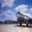
\includegraphics[width = 0.09 \textwidth]{images/datasets/cifar10_0.png}
    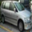
\includegraphics[width = 0.09 \textwidth]{images/datasets/cifar10_1.png}
    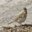
\includegraphics[width = 0.09 \textwidth]{images/datasets/cifar10_2.png}
    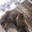
\includegraphics[width = 0.09 \textwidth]{images/datasets/cifar10_3.png}
    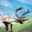
\includegraphics[width = 0.09 \textwidth]{images/datasets/cifar10_4.png}
    
\includegraphics[width = 0.09 \textwidth]{images/datasets/cifar10_5.png}
    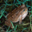
\includegraphics[width = 0.09 \textwidth]{images/datasets/cifar10_6.png}
    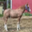
\includegraphics[width = 0.09 \textwidth]{images/datasets/cifar10_7.png}
    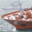
\includegraphics[width = 0.09 \textwidth]{images/datasets/cifar10_8.png}
    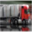
\includegraphics[width = 0.09 \textwidth]{images/datasets/cifar10_9.png}
   % 
\includegraphics[width = 0.09 \textwidth]{images/datasets/svhn_0.png}
    %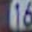
\includegraphics[width = 0.09 \textwidth]{images/datasets/svhn_1.png}
    %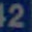
\includegraphics[width = 0.09 \textwidth]{images/datasets/svhn_2.png}
    %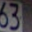
\includegraphics[width = 0.09 \textwidth]{images/datasets/svhn_3.png}
    %
\includegraphics[width = 0.09 \textwidth]{images/datasets/svhn_4.png}
    %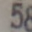
\includegraphics[width = 0.09 \textwidth]{images/datasets/svhn_5.png}
    %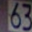
\includegraphics[width = 0.09 \textwidth]{images/datasets/svhn_6.png}
    %
\includegraphics[width = 0.09 \textwidth]{images/datasets/svhn_7.png}
    %\includegraphics[width = 0.09 \textwidth]{images/datasets/svhn_8.png}
    %\includegraphics[width = 0.09 \textwidth]{images/datasets/svhn_9.png}
    \includegraphics[width = 0.09 \textwidth]{images/datasets/emnist_0.jpg}
    \includegraphics[width = 0.09 \textwidth]{images/datasets/emnist_1.jpg}
    \includegraphics[width = 0.09 \textwidth]{images/datasets/emnist_2.jpg}
    \includegraphics[width = 0.09 \textwidth]{images/datasets/emnist_3.jpg}
    \includegraphics[width = 0.09 \textwidth]{images/datasets/emnist_4.jpg}
    \includegraphics[width = 0.09 \textwidth]{images/datasets/emnist_5.jpg}
    \includegraphics[width = 0.09 \textwidth]{images/datasets/emnist_6.jpg}
    \includegraphics[width = 0.09 \textwidth]{images/datasets/emnist_7.jpg}
    \includegraphics[width = 0.09 \textwidth]{images/datasets/emnist_8.jpg}
    \includegraphics[width = 0.09 \textwidth]{images/datasets/emnist_9.jpg}
    %\includegraphics[width = 0.09 \textwidth]{images/datasets/stl10_0.png}
    %\includegraphics[width = 0.09 \textwidth]{images/datasets/stl10_1.png}
    %\includegraphics[width = 0.09 \textwidth]{images/datasets/stl10_2.png}
    %\includegraphics[width = 0.09 \textwidth]{images/datasets/stl10_3.png}
    %\includegraphics[width = 0.09 \textwidth]{images/datasets/stl10_4.png}
    %\includegraphics[width = 0.09 \textwidth]{images/datasets/stl10_5.png}
    %\includegraphics[width = 0.09 \textwidth]{images/datasets/stl10_6.png}
    %\includegraphics[width = 0.09 \textwidth]{images/datasets/stl10_7.png}
    %\includegraphics[width = 0.09 \textwidth]{images/datasets/stl10_8.png}
    %\includegraphics[width = 0.09 \textwidth]{images/datasets/stl10_9.png}
    \includegraphics[width = 0.09 \textwidth]{images/datasets/cinic10_0.jpg}
    \includegraphics[width = 0.09 \textwidth]{images/datasets/cinic10_1.png}
    \includegraphics[width = 0.09 \textwidth]{images/datasets/cinic10_2.png}
    \includegraphics[width = 0.09 \textwidth]{images/datasets/cinic10_3.png}
    \includegraphics[width = 0.09 \textwidth]{images/datasets/cinic10_4.png}
    \includegraphics[width = 0.09 \textwidth]{images/datasets/cinic10_5.png}
    \includegraphics[width = 0.09 \textwidth]{images/datasets/cinic10_6.png}
    \includegraphics[width = 0.09 \textwidth]{images/datasets/cinic10_7.png}
    \includegraphics[width = 0.09 \textwidth]{images/datasets/cinic10_8.png}
    \includegraphics[width = 0.09 \textwidth]{images/datasets/cinic10_9.png}
    \caption{Representative examples for each class from the training sets of MNIST, CIFAR-10, EMNIST and CINIC-10.}
    \label{fig:datasets}
\end{figure}

\section{Neural Networks}
We use eight different neural networks for our experiments, from which four are trained on CIFAR-10 and another four on MNIST, as the different complexities of the datasets (grayscaled handwritten digits and real-world images) require different types of models. 

%ordered by age
\begin{itemize}
    \item \textbf{LeNet \cite{lecun_gradient-based_1998}} is a group of CNNs developed by Yann LeCun in the 1998. LeNets consist of two convolutional layers, two pooling layers and one (LeNet-1), two (LeNet-4) or three  (LeNet-5) dense layers. An illustration of the original architecture of LeNet-5 is shown in \cref{fig:lenet5}. In our experiments, we use LeNet-1, LeNet-3 and LeNet-5 for training on MNIST. LeNet-3 is a variation of the original LeNet-4 with six instead of four filters in the first convolutional layer. In our implementation, we used max-pooling for downsampling, but also average-pooling is quite common to use.
    
    \item \textbf{ResNet \cite{he_deep_2016}} stands for Residual Network. ResNets solve the problem of \textit{vanishing gradient}, i.e. the problem of when a network has too many layers, the gradients of the loss function can get zero, thus weights would not get updated and the network would not learn. ResNets counter this problem by utilizing \textit{skip connections} (also called \textit{shortcuts}) to jump over some layers. In our experiments, we use ResNet-18, ResNet-34 and ResNet-50 and train on CIFAR-10. The architectures differ in the number of layers. The number indicates the number of layers: ResNet-18 consists of 18 layers, ResNet-34 of 34 layers, etc. An illustration of a ResNet-18 is shown in \cref{fig:arch-resnet18}.
    
    \item \textbf{DenseNet \cite{huang_densely_2017}} stands for Densely Connected Convolutional Networks. DenseNets are a type of neural networks that build on the ideas of ResNets. Instead of including skip connections, in DenseNets, each layer has direct access to the gradients of the loss function and the original input image, since each layer takes \textit{all} preceding feature-maps as input. A DenseNet architecture consists of several \textit{dense blocks}. Such a dense block is shown in \cref{fig:arch-densenet}, where one can see typical connections between each of the layers. We use the DenseNet-121 in our experiments for CIFAR-10. We sometimes use just the generic term DenseNet, but always mean DenseNet-121.
    %\item \textbf{VGG-16 \cite{simonyan_very_2015}:}
    
    \item \textbf{SimpleNet \cite{hasanpour_lets_2018}} is convolutional neural network consisting of $13$ layers. It was designed to be simple and reasonably deep and still perform similar to deeper and more complex architectures. We use SimpleNet for training on MNIST.
\end{itemize}

\begin{figure}
    \centering
    \includegraphics[width=0.9\linewidth]{images/arch/ResNet-18-model-architecture-10.png}
    \caption{ResNet-18 architecture. Source: \cite{almezhghwi_improved_2020}}
    \label{fig:arch-resnet18}
\end{figure}

\begin{figure}
    \centering
    \includegraphics[width=0.6\linewidth]{images/arch/densenet.png}
    \caption{A 5-layer dense block. A DenseNet consists of several dense blocks. Source: \cite{huang_densely_2017}}
    \label{fig:arch-densenet}
\end{figure}

\begin{figure}
    \centering
    \includegraphics[width=0.9\linewidth]{images/arch/lenet5.png}
    \caption{Architecture of LeNet-5. Source: \cite{lecun_gradient-based_1998}}
    \label{fig:lenet5}
\end{figure}

To get an idea for the complexity of the models, we summarised the amount of trainable parameters together with the benchmark test accuracies and the test accuracies of our trained models in \cref{tab:trainable_parameters}. We can see that the models trained on MNIST reach very high results: close to or above 99\% accuracy on the test set. The results for CIFAR-10 are around 95\% accuracy on the test set.

%\red{Would be good to add somewhere the state-of-the art results for the datasets (globally, i.e. also with models that you do NOT consider, and also with the chosen models)}

% consider this for footnotes in table:
%https://tex.stackexchange.com/questions/444467/footnote-after-the-table-and-not-before

\begin{table}
\small
%\setlength\tabcolsep{2.5pt}
%\renewcommand{\arraystretch}{1.5}

\begin{threeparttable}

    %\rowcolors{2}{white}{gray!15}
    \caption{Amount of trainable parameters and the state-of-the-art test accuracy, as well as, our test accuracy of the trained models.}
    \label{tab:trainable_parameters}
    
    \centering
    \begin{tabular}{|l|l|r|r|r|}
        \hline
        \textbf{Architecture} & \textbf{Dataset} & \textbf{Trainable parameters} & \textbf{Benchmark test acc.} & \textbf{Test acc.} \\
        \hline
        LeNet-1 & MNIST & 7,206 & 98.3\% \tnote{1} \, & 98.768\% \\
        \hline
        LeNet-3 & MNIST & 69,362 & - & 99.229\% \\
        \hline
        LeNet-5 & MNIST & 107,786 & 99.15\% \tnote{1} \, & 99.229\% \\
        \hline
        DenseNet-121 & CIFAR-10 & 3,272,856 & 95.04\% \tnote{2} \, & 94.581\% \\
        \hline
        SimpleNet & MNIST & 5,497,226 & 99.75\% \tnote{3} \, & 99.589\% \\
        \hline
        ResNet-18 & CIFAR-10 & 11,173,962 & 95.00\% \tnote{4} \, & 95.122\% \\
        \hline
        VGG-16 & CIFAR-10 & 14,857,034 & 92.63\% \tnote{5} \, & - \\
        \hline
        ResNet-34 & CIFAR-10 & 21,282,122 & 95.95\% \tnote{4} \, & 95.212\% \\
        \hline
        ResNet-50 & CIFAR-10 & 23,513,162 & 95.00\% \tnote{4} \, & 94.391\% \\
        \hline
    \end{tabular}
    
\medskip % some vertical separation
\begin{tablenotes}
\footnotesize  % nothing is optional in 'tablenotes'
\item[1] \label{note:lenet} \url{http://yann.lecun.com/exdb/mnist/}
\item[2] \url{https://github.com/kuangliu/pytorch-cifar}
\item[3] \url{https://paperswithcode.com/sota/image-classification-on-mnist}
\item[4] \url{https://github.com/mbsariyildiz/resnet-pytorch}
\item[5] \url{https://github.com/chengyangfu/pytorch-vgg-cifar10}

\end{tablenotes}


\end{threeparttable}
\end{table}


% ResNet-18/34/50: https://github.com/mbsariyildiz/resnet-pytorch
% DenseNet, ResNet-18 and ResNet-50 are taken from \url{https://github.com/kuangliu/pytorch-cifar}
% vgg16: https://github.com/chengyangfu/pytorch-vgg-cifar10
% simplenet: https://paperswithcode.com/sota/image-classification-on-mnist
% lenet1/5: http://yann.lecun.com/exdb/mnist/


%Benchmark results for DenseNet-121 are taken from \url{https://github.com/kuangliu/pytorch-cifar}, for ResNet-18/34/50 from \url{https://github.com/mbsariyildiz/resnet-pytorch}, for VGG-16 from \url{https://github.com/chengyangfu/pytorch-vgg-cifar10}, for SimpleNet from , and for LeNet-1/5 from \url{http://yann.lecun.com/exdb/mnist/}

% include configurations here

We train multiple versions of the watermarked models, varying the trigger set size, which are listed in \cref{tab:trg_set_sizes}. We choose a fixed ratio of the training set, to be able to compare the models for MNIST and CIFAR-10. Note that if the dataset is very large, then even a trigger set size of $0.02\%$ of the dataset size could be still (too) large. Therefore, it would be interesting for future work to evaluate the watermarking methods also on a substantially larger dataset. In this way, we could find out if the trigger set size must reach a specific ratio of the dataset size or requires an absolute number to be effective. Unfortunately, the difference in size between MNIST and CIFAR-10 is not enough for such an experiment.

\begin{table}
\small
    \centering
    \caption{Trigger set sizes used for training models with various watermarking methods.}
    %\rowcolors{2}{white}{gray!15}
    \begin{tabular}{|l|l|l|l|}
        \hline
        \textbf{Architecture} & \textbf{Dataset} & \textbf{Trigger set sizes} & \textbf{Ratio of dataset size}\\
        \hline
        DenseNet-121 & CIFAR-10 & 20, 100, 500 & 0.04\%, 0.2\%, 1\% \\
        \hline
        ResNet-18 & CIFAR-10 & 20, 100, 500 & 0.04\%, 0.2\%, 1\% \\
        \hline
        ResNet-34 & CIFAR-10 & 20, 100, 500 & 0.04\%, 0.2\%, 1\% \\
        \hline
        ResNet-50 & CIFAR-10 & 20, 100, 500  & 0.04\%, 0.2\%, 1\% \\
        \hline
        SimpleNet & MNIST & 12, 24, 120, 600 & 0.02\%, 0.04\%, 0.2\%, 1\% \\
        \hline
        LeNet-1 & MNIST & 24, 120, 600 & 0.04\%, 0.2\%, 1\% \\
        \hline
        LeNet-3 & MNIST & 24, 120, 600 & 0.04\%, 0.2\%, 1\% \\
        \hline
        LeNet-5 & MNIST & 24, 120, 600 & 0.04\%, 0.2\%, 1\% \\
        \hline
    \end{tabular}
    \label{tab:trg_set_sizes}
\end{table}

The trigger set sizes from \cref{tab:trg_set_sizes} are used for all watermarking methods, except \textit{WeaknessIntoStrength}, for which the authors provided a trigger set of only 100 images for download. For this method, we train with a trigger set size of 20 and 100 on \textit{all} architectures.
%Moreover, we train \textit{Blackmarks} on all architectures except ResNet-50 because of the limited GPU memory (cf. \cref{sec:blackmarks}).
This leads to a total number of \textbf{191 trained models}.

%7*3+4=25 modelle pro method
%25*7(methoden)=175
%16*1(weakness)= 16
%--------------------
%               191

%TODO: you need something like this to have a slightly less abrupt transition to the resource usage description. Maybe even add a sub-sub section?
\subsection{Training time}

All models were trained on a NVIDIA GeForce RTX 2080. To determine the overall training time, we show the training time for embedding the watermark and fine-tuning the watermarked models in \cref{tab:training_time}, exemplary for \textit{WeaknessIntoStrength} trained with $100$ trigger images. We can see from this table that the training time not only depends on the number of iterations, but also on the complexity of the model. For example, a ResNet-34 needs roughly 60\% of the time of a ResNet-50 with the same number of training iterations.
%It most probably depend on other properties as well, since a LeNet-1, e.g., trained for 100 iterations does not take 5 times as much time as trained for 20 iterations, but only around 2 times. % Achtung embedding hat 100 examples mehr im training... 
\begin{table}
\small
    \centering
    \caption{Embedding and fine-tuning time (with learning rate 0.01) for \textit{WeaknessIntoStrength} with 100 trigger images. The time is given in the format (hh:mm:ss).}
    %\rowcolors{2}{white}{gray!15}
\begin{tabular}{|l|l|r|r|r|r|}
\hline
\textbf{Arch} & \textbf{Dataset} & \textbf{Embedding} & \textbf{Iterations} & \textbf{Fine-tuning} & \textbf{Iterations} \\ \hline
DenseNet      & CIFAR-10         & 05:09:18                      & 190                 & 02:28:43                        & 100                     \\ \hline
ResNet-18     & CIFAR-10         & 02:28:46                      & 191                 & 01:21:00                                & 100                    \\ \hline
ResNet-34     & CIFAR-10         & 04:02:41                      & 195                 & 01:51:41                        & 100                    \\ \hline
ResNet-50     & CIFAR-10         & 06:16:30                      & 195                 & 02:40:16                        & 100                    \\ \hline
SimpleNet     & MNIST            & 00:14:12                      & 21                  & 00:40:26                        & 100                    \\ \hline
LeNet-1       & MNIST            & 00:06:31                      & 21                  & 00:13:11                        & 100                    \\ \hline
LeNet-3       & MNIST            & 00:06:41                      & 25                  & 00:13:09                        & 100                    \\ \hline
LeNet-5       & MNIST            & 00:06:47                      & 21                  & 00:13:42                        & 100                    \\ \hline
\hline
\textbf{Sum}           &                  & \textbf{18:31:26}                      &                     & \textbf{09:42:09}                                &                     \\ \hline
\end{tabular}
\label{tab:training_time}
\end{table}


%training: 18.5/8=2.3125 hours per model
% --> 191*2.3=440hours=18.4days
%finetuning: 9.7/8=1.2125 hours per model
% --> 1.2125*191=231.6hours=9.6days
% --> 9.6 * 2 = 19.2 days
% =========
% 18.4 + 19.2 = 37.6 days for training and finetuning
If we take $\frac{18.5}{8} \approx 2.3$ hours, as measured in \cref{tab:training_time}, as the average embedding time for one single model, we get a total embedding time of around $440$ hours or around $18.4$ days. An estimation of the total fine-tuning time (for one learning rate) results in around $9.6$ days, i.e. $19.2$ days for both learning rates (cf. \cref{sec:finetuning}). This gives us nearly \textbf{38 days} ($18.4+19.2=37.6$) of training to embed the watermark and performing the fine-tuning attacks. Note, that in this number we neither include the time for generating and verifying the watermarks, nor the time for the pruning attacks, nor the time used for the additional experiments for \textit{FrontierStitching} and \textit{WMEmbeddedSystems} (cf. \cref{sec:eval-watermark-spec-param}) and other experiments that we performed along the way when testing different parameters. The exact embedding and fine-tuning times for the additional experiments for \textit{FrontierStitching} and \textit{WMEmbeddedSystems} are listed in \cref{tab:extra_exp_time}, which adds another \textbf{16 days} for the additional experiments on top of the \textbf{38 days}, leading to a total of $54$ days of compute time.

\begin{table}
\small
\centering
\caption{Training times for additional experiments in format (dd:hh:mm:ss).}
\begin{tabular}{|l|c|c|c|c|}
\hline
\textbf{Method} & \textbf{\# models} & \textbf{Embedding} & \textbf{Fine-Tuning} & \textbf{Both}        \\ \hline
\textit{FrontierStitching}          & 56                 & 05:08:27:22        & 05:12:40:06          & 10:21:07:27          \\ \hline
\textit{WMEmbeddedSystems}          & 24                 & 02:06:52:53        & 02:17:10:32          & 05:00:03:25          \\ \hline
%Blackmarks                 & 35                 & 03:10:15:33        & 02:21:35:40          & 06:07:51:14          \\ \hline
\hline
\textbf{Sum}               &                    &                    &                      & \textbf{15:21:10:52} \\ \hline
\end{tabular}
\label{tab:extra_exp_time}
\end{table}

%For the experiments for \textit{FrontierStitching}, we trained $56$ models (8 architectures, varying 7 values for the parameter). The embedding time was 5.35 days and the fine-tuning time (for both learning rates) was 5.53 days. Resulting in 10.88 days for the extra experiments for \textit{FrontierStitching}.

%For the experiments for \textit{WmEmbeddedSystems}, we trained $24$ models (8 architectures, varying 3 values for the parameter). Embedding 2.286725023 days, finetuning 2.715647254 days

%For the experiments for \textit{Blackmarks}, we trained $35$ models (7 architectures, varying 5 values for the parameter). Embedding 3.427469521, finetuning 2.899774066

\section{Setting hyperparameters}

We specify the hyperparameters for training the models in \cref{tab:hyperparameter_config}. We choose this configuration based on training non-watermarked models on a few different configurations and selecting the model with the minimal validation loss. We test different configurations by varying between the SGD and Adam optimiser as well as the \texttt{MultiStepLR} and \texttt{CosineAnnealingLR}, which are both commonly used learning rate schedulers. We test the default learning rate for the optimiser, which is $\alpha=0.1$ for SGD and $\alpha=0.001$ for Adam, and kept those as we reached results comparable to the benchmarks (cf. \cref{tab:trainable_parameters}). We use this hyperparameters configuration for training the non-watermarked models as well as the watermarked models.

\begin{table}
\small
\centering
\caption{Hyperparameters configuration for the architectures. \textbf{lr} stands for learning rate, \textbf{bs} for batch size, \textbf{wm\_bs} for watermarking batch size, i.e. the batch size for the trigger set, and \textbf{epochs} the number of training iterations.}

\setlength\tabcolsep{4pt}

%\rowcolors{2}{white}{gray!15}
\begin{tabular}{|l|l|c|l|c|c|c|}
\hline
\textbf{Architecture} & \textbf{optimizer} & \textbf{lr} & \textbf{scheduler} & \textbf{bs} & \textbf{wm\_bs} & \textbf{epochs} \\ \hline
DenseNet-121   & \gape{\makecell[l]{SGD \\ mom.=0.9 \\ decay=0.0005}} & 0.1     & \gape{\makecell[l]{CosineAnnealingLR \\ T\_max=200}} & 64 & 32 & 200      \\ \hline
ResNet-18      & \gape{\makecell[l]{SGD \\ mom.=0.9 \\ decay=0.0005}} & 0.1     & \gape{\makecell[l]{CosineAnnealingLR \\ T\_max=200}} & 64 & 32 & 192      \\ \hline
ResNet-34      & \gape{\makecell[l]{SGD \\ mom.=0.9 \\ decay=0.0005}} & 0.1     & \gape{\makecell[l]{CosineAnnealingLR \\ T\_max=200}} & 64 & 32 & 195      \\ \hline
ResNet-50      & \gape{\makecell[l]{SGD \\ mom.=0.9 \\ decay=0.0005}} & 0.1     & \gape{\makecell[l]{CosineAnnealingLR \\ T\_max=200}} & 64 & 32 & 192      \\ \hline
SimpleNet      & \gape{\makecell[l]{SGD \\ mom.=0.9 \\ decay=0.0005}} & 0.1     & \gape{\makecell[l]{MultiStepLR \\ n=20, gamma=0.1}}  & 64 & 32 & 24       \\ \hline
LeNet-1        & ADAM                                                 & 0.001   & \gape{\makecell[l]{MultiStepLR \\ n=20, gamma=0.1}}  & 64 & 32 & 48       \\ \hline
LeNet-3        & \gape{\makecell[l]{SGD \\ mom.=0.9 \\ decay=0.0005}} & 0.1     & \gape{\makecell[l]{MultiStepLR \\ n=20, gamma=0.1}}  & 64 & 32 & 55       \\ \hline
LeNet-5        & \gape{\makecell[l]{SGD \\ mom.=0.9 \\ decay=0.0005}} & 0.1     & \gape{\makecell[l]{MultiStepLR \\ n=20, gamma=0.1}}  & 64 & 32 & 42       \\ \hline
\end{tabular}
\label{tab:hyperparameter_config}
\end{table}


\subsection{Setting watermark-specific hyperparameters} \label{sec:studysettings:watermark-spec}

Some of the papers, e.g. \cite{guo_watermarking_2018}, do not mention all of the specific parameters that were used in their experiments. We, therefore, have to experimentally find the optimal parameters for those watermarking methods. We introduce a \textit{ranking system} that helps us to decide on the optimal parameters. 

For the experiments, we first fix the trigger set size to 100, as $100$ is a trigger set size commonly used in related work, and then train several models, varying one parameter at a time. We train on all architectures and perform pruning attacks as well as fine-tuning attacks. In this manner, we can evaluate the fidelity and robustness of the different models.

Every model for each watermarking method will be evaluated in three categories: \textit{fidelity}, \textit{robustness against pruning}, \textit{robustness against fine-tuning}. The ranking systems works as follows: for each category, the model with the best evaluation gets the $n$ points (where $n$ is the number of different values for the varied parameter) and the one with the lowest performance in the category gets one point. The points are summed up across the categories resulting in a ranking for each of the parameter's values. 

For fidelity, the performance is measured by the difference of the test accuracy compared to the non-watermarked model and for robustness against fine-tuning or pruning, by the watermark accuracy after a fine-tuning attack or pruning attack.

Note that we weight all three categories equally. One can argue that, e.g, robustness is the most important property and would therefore weight this category stronger, but such a weighting is very much dependent on the general setting and threat model in which the watermark is being employed. We, therefore, refrain from optimising to a specific assumption. 

%The evaluation of performance for fidelity and robustness against fine-tuning is straight forward, but for robustness against pruning, it is not. For fidelity, the performance is measured by the difference of the test accuracy compared to the non-watermarked model.For robustness against fine-tuning, we compare to the watermark accuracy after a fine-tuning attack. For robustness against pruning, we evaluate the models depending on the watermark accuracy after the pruning attack. We consider the pruning attack as plausible if the attack does degrade the model's test accuracy only at the maximum of $3.5\%$, since an attacker would not use a model that is significantly degraded. Therefore, we choose the maximum pruning rate at which the test accuracy does not fall under this threshold and then compare the watermark accuracies. We chose 3.5\% as a value also in accordance with \cite{liu_trojaning_2017}; for example, \cite{liu_fine-pruning_2018} chose a very similar value of 4\% when defending against backdoors, which is essentially the same task as removing a watermark based on backdoors.

%---> i'll explain how the selection of a plausible pruning attack works later in some section about pruning...

%TODO: it is not clear why pruning and fine-tuning are differently treated in the evaluation. For both, the test accuracy will fall; the difference is rather in the selection which attack setting you consider (and for both, one could consider the 4% threshold as whether the attack is successful or not)




\chapter{Empirical comparison of existing watermarking methods} \label{ch:empirical_comparison}
In this chapter, we present the implementation in \cref{sec:implementation}, where the watermarking methods are discussed in more detail, and the evaluation in \cref{sec:evaluation}, where we present the results and evaluate the watermarking methods.

\section{Implementation} \label{sec:implementation}
For an independent comparison of watermarking methods, we implement and compare them in a common framework. We implement or adapt, if there was an existing implementation, the chosen watermarking methods in Python 3.7.10 using PyTorch 1.8.1. A complete list of dependencies is provided in \cref{sec:dependencies}. The implementation and results can be found in the GitHub project \url{https://github.com/mathebell/model-watermarking}.


\subsection{Framework for watermarking methods}
In this section, we present the framework that we used and discuss the watermarking methods in more detail, focusing on the implementation.

\begin{algorithm}[H]
\caption{General framework}\label{algo:framework}
\begin{algorithmic}[1]
\REQUIRE dataset $\mathcal{D}$, initialised or pre-trained model $\mathcal{F}_{\mathbf{w}}$, hyperparameters $\beta$
\ENSURE watermarked model $\mathcal{F}_{\mathbf{w}}^{M}$, trigger set $\mathcal{T}$

\STATE $\mathrm{wm\_method} \gets WMMethod.init(\beta)$

\STATE $\mathcal{T} \gets \mathrm{wm\_method}.gen\_watermark(\mathcal{F}_{\mathbf{w}}, \mathcal{D})$

\STATE $\mathcal{F}_{\mathbf{w}}^{M} \gets \mathrm{wm\_method}.embed\_watermark(\mathcal{F}_{\mathbf{w}}, \mathcal{D}, \mathcal{T})$

\STATE $\mathrm{wm\_acc} \gets \mathrm{wm\_method}.verify\_watermark(\mathcal{F}_{\mathbf{w}}^{M}, \mathcal{T})$
\IF {wm\_acc $\geq$ threshold}
    \PRINT Watermark was verified.
\ELSE 
    \PRINT Watermark was not verified.
\ENDIF
\end{algorithmic}
\end{algorithm}

\cref{algo:framework} describes the general framework that was used for all the watermarking methods. \textit{WMMethod} stands for the class of a watermarking method. Each of the watermarking methods are implemented in their own class, namely:
\begin{itemize}
    \item \textit{WeaknessIntoStrength} \cite{adi_turning_2018}
    \item \textit{ProtectingIP} \cite{zhang_protecting_2018}
    \item \textit{PiracyResistant} \cite{li_piracy_2020}
    \item \textit{ExponentialWeighting} \cite{namba_robust_2019}
    \item \textit{FrontierStitching} \cite{merrer_adversarial_2019}
    \item \textit{WMEmbeddedSystems} \cite{guo_watermarking_2018}
    %\item \textit{Blackmarks} \cite{chen_blackmarks_2019}
\end{itemize}

The meaning and usage of each of the member functions, i.e. functions that are defined inside the class, in \cref{algo:framework} are the following:

\begin{itemize}
    \item \textit{WMMethod.init}($\beta$) initialises the watermarking method depending on the given hyperparameters that are represented by $\beta$. The hyperparameters consist of network specific parameters like, e.g., the batch size for the training set (batch\_size), the number of training iterations without watermarks (epochs\_wo\_wm) and the learning rate $\alpha$, and parameters that are specifying the watermarking method, e.g. the batch size for the trigger set (wm\_batch\_size), the embedding type (embed\_type) and the trigger set size (trg\_set\_size).
    
    \item \textit{WMMethod.gen\_watermark}($\mathcal{F}_{\mathbf{w}}, \mathcal{D}$) generates the trigger set $\mathcal{T}$. The trigger set is mostly generated using the original dataset $\mathcal{D}$ and, e.g., placing a trigger pattern onto the image. In some cases such as perturbation based watermarking methods, the watermark generation process makes use of the model itself $\mathcal{F}_{\mathbf{w}}$ and is, therefore, also passed to the function.
    
    \item \textit{WMMethod.embed\_watermark}($\mathcal{F}_{\mathbf{w}}, \mathcal{D}, \mathcal{T}$) embeds the watermark into the model, i.e. trains the model, besides on the original dataset $\mathcal{D}$, also on the trigger set $\mathcal{T}$. The model is either first trained on the original training set and then fine-tuned with the union of the original training set and the trigger set, or it is trained from the beginning with the unified set. The output of this function is the watermarked model $\mathcal{F}_{\mathbf{w}}^{M}$.
    
    \item $WMMethod.verify\_watermark(\mathcal{F}_{\mathbf{w}}^{M},\mathcal{T})$: verifies the watermark. It tests the trigger set $\mathcal{T}$ on the watermarked model $\mathcal{F}_{\mathbf{w}}^{M}$, i.e. it passes the trigger set to the watermarked model and compares the output of the model with the trigger labels. The output of the function is the accuracy of the model on the trigger set, the watermark accuracy. The threshold, which decides if a watermark can be verified or not, has to be specified in the hyperparameters $\beta$.
    %can either be a boolean, \texttt{True} or \texttt{False}, as the answer to the question if the watermark can be verified, or it can output the watermark accuracy, the fraction of correctly classified trigger images. If the output shall be a boolean, we have to specify the watermark accuracy threshold in the hyperparameters $\beta$. Then, the output is \texttt{True} when the watermark accuracy is above the watermark accuracy threshold.
\end{itemize}

As the watermarking methods differ very much on the used trigger images, the function $gen\_watermark()$ is the most customised one. We explain this function for each of the watermarking methods in the following sections.




\subsubsection{WeaknessIntoStrength}
\label{sec:weakness}

This method uses out-of-distribution trigger images (OOD). The authors of this method choose a set of abstract images that are completely unrelated to the original dataset (cf. \cref{fig:trigger-a}) and provided them for download. The trigger set is specifically constructed and is, unfortunately, limited to 100 images, which imposes limitations in the experiment setup. For this method, we thus train the models only with a trigger set size of $20$ and $100$.
%Unfortunately, we do not train WeaknessIntoStrength with $500$ (for CIFAR-10) or $600$ (for MNIST) trigger images, since we would have to search for another $500$ "abstract" images. The choice of trigger images has much influence on the behaviour of the watermarked models (cf. \cref{sec:evaluation}) and we do not have any information on how the authors assessed the trigger set.
However, the method ProtectingIP-OOD serves as an alternative for this method, since it also uses out-of-distribution trigger images, but not "abstract" ones (cf. \cref{sec:protecting}).
%We will compare those two methods later on in \cref{sec:evaluation}.

The authors compare two different embedding types, namely \textit{pretrained} and \textit{fromscratch}. \textit{Pretrained} means that the watermarks are embedded in a fine-tuning process, \textit{after} the model was already trained and has converged on the clean training set. The pre-trained model is then fine-tuned with the union of the training dataset and the trigger set. When embedding \textit{fromscratch}, we train the model from the beginning with the union of the training dataset and the trigger set. We also used both embedding types for this method and compare the results in \cref{sec:compare-results:weakness}.

Since the trigger images are already provided and do not have to be generated, the function \textit{WeaknessIntoStrength.gen\_watermark}($\beta$) only loads the right amount of trigger images from their storage location (specified by the trigger set size in $\beta$).

%paper: "Machen in paper auch transfer learning mit "labelled part of STL-10" für 20 epochen."


\subsubsection{ProtectingIP} 
\label{sec:protecting}

This method considers three watermarking types, namely pattern, noise and OOD:
\begin{itemize}
    \item \textbf{Pattern} trigger images are created by placing a simple text "TEST" in the colour grey on the bottom part of random images from the training dataset (cf. \cref{fig:trigger-c}).
    \item \textbf{Noise} based trigger images are created by placing a random noise on a random subset of images from the training dataset (cf. \cref{fig:trigger-d}).
    \item \textbf{OOD} trigger images are formed by a subset of the MNIST dataset for training on CIFAR-10 and vice versa.
\end{itemize}

The watermarking type is specified in the hyperparameters $\beta$ and the function \textit{ProtectingIP.gen\_watermark}($\beta$) performs the trigger set generation based on the specified watermarking type. The watermark is embedded by training the model from scratch on the union of the original training dataset and the trigger set.

%paper: "Fine-tuning: As we discussed in Section 2, training a well- designed deep neural network from scratch requires a large training dataset, while insufficient data can greatly affect the DNNs’ perfor- mance. Therefore, more often in practice, it will be easy to fine-tune existing start-of-the-art models when sufficient training data is not available [43, 56]. In general, if the dataset is not dramatically dif- ferent in context from the dataset which the pre-trained model is trained on, fine-tuning is a good choice. Therefore, fine-tuning can be a very effective approach for plagiarizer to train a new model on top of the stolen model with only fewer new training data. In this way, the new model can inherit the performance of the stolen model, but also looks different from the stolen model."

\subsubsection{PiracyResistant}
\label{sec:piracy}

This watermarking method relies on an advanced pattern generation. First, a binary pattern is created based on a unique signature, which serves as an additional security measure. As already discussed in \cref{sec:black-box:pattern}, the method uses what the authors call \textit{dual embedding}: the model is trained to classify (i) data with a pre-defined binary pattern correctly (called the \textit{null embedding}), i.e. an image with the pattern gets assigned the original label, and (ii) data with an inverted pattern (binary bits are switched) incorrectly (called the \textit{true embedding}), i.e. an image with the inverted pattern gets assigned a different label.
%The pattern is placed on random images from the original training dataset. Half of the trigger set, then, has the pattern embedded on the images with the original image's label, the true label, and the other half of the trigger set has the inverted pattern embedded with a different label.
This label is also defined by the unique signature. Note that the watermark embedding consists of two parts, the null and true embedding, thus dual embedding does not mean that two watermarks are embedded.

The pattern size is fixed to $6\times6$ pixels and $\lambda$, the strength of pixel change, to 2000, as suggested by the paper's authors.

%paper: "Tranfer-learning: The dataset we use for the student task is LISA which has 3,987 training images and 340 testing im- ages of 17 US traffic signs. We resize all the images to (48, 48, 3) for transfer learning purpose. During the transfer learn- ing process, we fine tune the student model for 200 epochs using student training data, using SGD optimizer with 0.01 learning rate and 0 decay."

%"While model extraction attacks could produce a watermark-free version of the model, our analysis be- low shows that they do not qualify as a feasible attack against our watermark design given their data requirements."

%"Neural Cleanse is unable to detect any “backdoor” (aka watermark) on our watermarked models (see Table 5). All watermarked models return values lower than the recom- mended threshold of 2, and in all but one case, the anomaly index of the watermarked model is lower than that of the orig- inal (watermark-free) model. This is because Neural Cleanse (and followup work) assume that backdoors are small input perturbations that create large changes in the feature space, and detect these behaviors as anomalies. Since our true and null embeddings use extreme values −λ and λ, they repre- sent large perturbations in the input space (L2 distance) that affect the feature space. Thus they do not show up as any anomalies to Neural Cleanse."

\subsubsection{ExponentialWeighting}
\label{sec:exponential}

This method uses in-distribution trigger images, i.e. images from the training dataset, but purposely labelled wrongly. The trigger label is the next label after the true label in the dataset's \textit{label vector}. For example, the label vector for CIFAR-10 is [airplane, car, bird, cat, deer, dog, frog, horse, ship, truck]. The function \textit{ExponentialWeighting.gen\_watermark}($\beta$) randomly samples the trigger set from the original trigger set and assigns the trigger labels in the previously explained manner.

In this method, the model is first trained on the clean training data, i.e. without trigger images. Alternatively, a pre-trained benchmark model is loaded. Then, the exponential weighting is activated in the layers. In every layer, the weights are transformed in the forward pass by \cref{eq:exponential-weighting}. We set $\lambda=2$, as it was used in the authors' experiments. We implemented the exponential weighting in PyTorch by creating sub-classes of the convolutional and feed-forward layer classes. To these sub-classes, we added member functions that activate and deactivate the exponential weighting, i.e. the additional transformation in the forward pass. We used these sub-classes of layers for all architectures, since they work as usual layers when not activated, thus not harming the other watermarking methods.

%"For our first contribution, we demonstrate a novel attack against water- marks, which we call query modification processing"

\subsubsection{FrontierStitching}
\label{sec:frontier}

This method is perturbation based. The trigger images are created as adversarial examples of the non-watermarked pre-trained model. The adversarial examples are created by the Fast Gradient Sign Method (FGSM). FGSM expects a parameter $\epsilon$, which controls the intensity of the adversarial perturbation. As a next step, the adversarial examples are divided into \textit{true} and \textit{false} adversarials\footnote{The publication calls them true and false \textit{adversaries}. We, however, call the attacker of the model an adversary and therefore choose the term \textit{adversarial}.} (cf. \cref{fig:merrer}). A \textit{true} adversarial is an adversarial example for which the model predicts a different label than the original true label. A \textit{false} adversarial, on the other hand, is an adversarial example for which the model still predicts the original true label, i.e. the adversarial image did not manage to fool the model. Both true and false adversarials are saved as trigger images, with the original true label as the trigger label. The sets of true and false adversarials have the same size, each constituting half of the trigger set size.
%The true and false adversarials build two equal parts of the trigger set.

We would find it interesting to analyse how the perturbation parameter $\epsilon$ influences the behaviour of the watermarked model. We therefore vary $\epsilon$ in our experiments (cf. \cref{sec:eval-param:frontier}). For the main analysis, however, we choose $\epsilon=0.25$ as the default parameter, following the authors' experiments.

\subsubsection{WMEmbeddedSystems}
\label{sec:embedded}

This method is pattern based. The pattern is created based on a unique signature, and subsequently then embedded with strength $\lambda$. Given the original image $\mathbf{X}$, the pattern $p$ and the strength $\lambda$, the trigger image is created by
\begin{align}
    \mathbf{X}^{\mathrm{trg}} = \mathbf{X} + \lambda p
\end{align}

Two hyperparameters that can be varied in this method are $\lambda$ -- the magnitude or strength of the pattern on the trigger images -- and the number of bits embedded in the trigger images. We fixed the number of bits to 128, following the authors. For $\lambda$ we performed several experiments in \cref{sec:eval-param:embedded}, to find an appropriate value for $\lambda$, as the authors did not provide such information in their paper.

%We assume that attackers are those who want to use a “pirate model” without paying the royalty. The attackers do not have the computa- tion power and technical expertise to train a model of their own. Uchida et al. argue that transfer learning and model compression operations, in particular, should be considered as possible types of attacks [6]. We do not consider them a type of threat for the follow- ing reasons. First, the cost of fine-tuning and compression is on the same order of magnitude as the cost of training, if not higher [13]. With that much resources and expertise at hand, an attacker would have built a model on their own. Second, a fine-tuned model is essentially a different model with certain initialization. In our own experiment for fine-tuning between different datasets, we observe up to 93% difference in average magnitude of weights in a layer. Not to mention that model architecture may be changed during the pruning of a model [14][2]. We argue the proof-of-authorship during actual model usage and “proof-of-origin” of a model should be two different problems. It is questionable whether the original model author can claim the authorship of a fine-tuned model, and thus our assumption.


%\subsubsection{Blackmarks}
%\label{sec:blackmarks}

%This watermarking method has the most advanced algorithm in our comparison. It is perturbation based, and encodes a unique signature $\mathbf{b} \in \{0,1\}^K$ within the distribution of the output activations, with $K$ being the trigger set size. We, however, only implement the method's trigger set generation and embedding, and do not focus on verification via output activations, since these activations are often not available in a black-box setting. The verification is performed exactly as in the other watermarking methods. We test the trigger set on the watermarked model and measure the watermark accuracy.

% encoding scheme:
%As a first step, the classes of a dataset are clustered into two categories. For every class, we pass all images from that class through the pre-trained model, and save the output activation vectors for the corresponding class. After iterating over all images of a class, we compute the mean value over all saved activation vectors. We repeat this for all classes and get a list of $n$ averaged activation vectors, where $n$ is the number of classes. This data is then fed into k-means clustering, which splits the data into two clusters depending on the averaged activation vectors. Now, every class corresponds to either bit 0 or bit 1. This mapping from class to bit is called the \textit{encoding scheme} and denoted by $\phi$.

% watermark generation:
%As a second step, for all images corresponding to the same bit, we create adversarial examples by using FGSM. Those adversarial examples are assigned with a trigger label, which is a randomly chosen label from the classes corresponding to the respective other bit. We create as many trigger images as defined by the trigger set size.


% embedding:
%The watermark embedding is then performed by training on the union of the original training dataset and the trigger set with a regularised loss function. The regulariser term measures the difference between the extracted signature from the output activations by \textit{decode\_predictions()} and the true signature $\mathbf{b}$:
%\begin{align}
%    \mathcal{L}_R = \mathcal{L}_0 + \lambda \mathcal{L}_{\mathrm{WM}} ( \mathbf{b}, decode\_predictions(\mathcal{F}_{\mathbf{w}}^{\mathrm{WM}}(\mathbf{X}^{\mathrm{trg}}), \phi))
%\end{align}
%We choose the embedding strength parameter as $\lambda=2$, as it was suggested in the paper.

%For this scheme, we need to set the parameter $\epsilon$ for FGSM, which controls the intensity of the adversarial perturbation. The authors do not provide the exact value for $\epsilon$ and therefore we perform several experiments in \cref{sec:eval-param:blackmarks} in order to find an appropriate value for $\epsilon$.

%It is worth noting that this advanced method is computationally the most expensive one. The GPU memory of 11GB was not enough for watermarking a ResNet-50. The source of the error is probably due to the non-optimal implementation, it occurs when computing the regulariser term of the loss function. In our implementation, we pass the whole trigger set through the model at once. This could have been avoided by also batching the trigger set for the computation of the regulariser term.



%TODO: describe whether the authors of the method would have had a similar issue, or that their models are smaller, and thus it likely didn't matter for them.
% Also be sure to discuss whether the memory issues occur due to the non-optimal implementation, or whether they are due to the algorithm itself (as it needs e.g. everything in memory at the same time)
% Also use this somewhere in your analysis - the memory requirement limits the applicability of the method


\subsection{Attacks} \label{sec:implementation_attack}

We provide a list of attacks that are used in the papers in \cref{tab:attacks_per_method}. We can see from that table that most of the papers test their watermarking methods against pruning and fine-tuning. \textit{ExponentialWeighting} presents their own attack \textit{Query Modification}, a watermark invalidation. It detects if the queried sample is a trigger image by applying an autoencoder. If the model predicts for the changed image a different label than for the queried image, it probably is a trigger image and the prediction for the changed image is returned.
%first detects if the queried sample is a trigger image and subsequently modifies the query image by applying an autoencoder.
They test it on several other methods and confirm that for \cite{zhang_protecting_2018, merrer_adversarial_2019, rouhani_deepsigns_2019} the watermark accuracy after a query modification is very low and therefore introduce a new watermarking method, which resists this kind of attack. The authors of \textit{WMEmbeddedSystems} do not use pruning or fine-tuning, as they assume that a user of the watermarked model and thus a possible attacker would not have enough computational power or technical expertise for such an attack, otherwise they would have trained their own model. As a second argument, they state that a fine-tuned model is a different model and it is questionable whether the model owner can claim the ownership of a fine-tuned model.  

\begin{table}
\caption{Attacks used in the papers.}
\label{tab:attacks_per_method}
\begin{threeparttable}

\resizebox{\textwidth}{!}{
\begin{tabular}{|l|c|c|l|}
\hline
                     & \textbf{Pruning}                   & \textbf{Fine-Tuning}              & \textbf{Other attacks?}                           \\ \hline
\textit{WeaknessIntoStrength} \cite{adi_turning_2018} &                           & \checkmark (STL-10) &                                         \\ \hline
\textit{ProtectingIP} \cite{zhang_protecting_2018}         & \checkmark & \checkmark \tnote{1} &                                         \\ \hline
\textit{PiracyResistant} \cite{li_piracy_2020}     & \checkmark & \checkmark \tnote{2} & \begin{tabular}[c]{@{}l@{}}Neural Cleanse \cite{wang_neural_2019},\\ Model Extraction Attack \cite{tramer_stealing_2016},\\ Piracy Attack \end{tabular} \\ \hline
\textit{ExponentialWeighting} \cite{namba_robust_2019} &                           &                           & Query Modification \cite{namba_robust_2019}                     \\ \hline
\textit{FrontierStitching} \cite{merrer_adversarial_2019}   & \checkmark & \checkmark \tnote{2} &                                         \\ \hline
\textit{WMEmbeddedSystems} \cite{guo_watermarking_2018}   &                           &                           &                                         \\ \hline
%Blackmarks \cite{chen_blackmarks_2019}          & \checkmark & \checkmark & Watermark Overwriting \cite{uchida_embedding_2017}                   \\ \hline
\end{tabular}
}

\medskip % some vertical separation
\begin{tablenotes}
\footnotesize  % nothing is optional in 'tablenotes'
\item[1] use half of the original test set for fine-tuning and the other half for evaluating the model
\item[2] do not specify the dataset for fine-tuning

\end{tablenotes}


\end{threeparttable}

\end{table}

% papers that consider pruning attack/model compression:
% blackmarks: ja
% wmembedded systems: no. argumentation: it is essentially another model
% frontier stitching: ja
% exponential: jein, machen glaub ich ne abwandlung bzw. eigene attacke
% piracy: ja
% protecting: ja
% weakness: nein, nur finetuning

\subsubsection{Parameter Pruning} \label{sec:implementation:pruning}
Since many of the papers (cf. \cref{tab:attacks_per_method}) considered parameter pruning as a valid attack for testing robustness, we implemented this attack as well. 

For this attack, we take the watermarked model and set those weights that have the smallest absolute value to zero. We vary the \textit{pruning rate} -- the rate of weights that are pruned in the model -- between $10\%$ and $90\%$ with a step-size of $10$ percentage points.

We consider the pruning attack as plausible if the attack does degrade the model's test accuracy only at the maximum of $3.5\%$, since an attacker would likely not use a model that is significantly degraded. Therefore, we choose the maximum pruning rate at which the test accuracy does not fall under this threshold and then compare the watermark accuracies. We chose 3.5\% as a value in accordance to \cite{liu_trojaning_2017}; for example, \cite{liu_fine-pruning_2018} chose a very similar value of 4\% when defending against backdoor attacks, which is essentially the same task as removing a watermark based on backdoors.

Note that there is also a different notion of pruning, also called \textit{fine-pruning} \cite{liu_fine-pruning_2018}, that relies on the availability of a clean set, to prune by activation value. This could also be a potential threat for the watermark, however, we keep this for future work.

\subsubsection{Fine-Tuning} \label{sec:finetuning}

Fine-tuning is another common attack. Some of the papers fine-tune on the same dataset (without trigger set) as the training was done, others use a different and smaller dataset and some do not mention which dataset was used (cf. \cref{tab:attacks_per_method}). As we assume that an attacker would not have access to the original training data, or only to a portion of it, we perform fine-tuning on a different, but similar dataset. The EMNIST dataset consists of different images than MNIST, but was build from the same database NIST, while around 22 \% of the CINIC-10 dataset consist of CIFAR-10 images, the other part of ImageNet. Fine-tuning with EMNIST and CINIC-10, therefore, simulates a strong attack, as we assume that the attacker knows the distribution of the original dataset. Our fine-tuning datasets do originally consist of more example-labels pairs, but we randomly downsample them to the same size as the original training set, as we assume that an attacker would have less or the same amount of data at most. 

Fine-Tuning is usually performed with a smaller learning rate than training, to not "overwrite" too much of the previously learned knowledge. Different learning rates achieve different success, as we analyse in \cref{sec:finetuning-experiments}. For the evaluation, we choose both a smaller learning and a larger learning rate. A smaller learning rate would correspond to \textit{transfer-learning}, and a larger learning rate rather to \textit{re-training}. Transfer learning aims to exploit the fact that the trained model generalises well and requires little adaption to the new task -- with a small learning rate only small changes are made to the model. On the other hand, re-training would mean that the model learns the new dataset from scratch and forgets the old dataset. We will discuss this phenomenon in more detail in \cref{sec:finetuning-experiments}. We implemented both attacks since they have different motivations and are plausible attacks -- transfer learning could happen as an accidental attack and re-training as an attack for purposefully removing the watermark. One could argue that this is not a plausible attack, since the model forgets the old dataset and the attacker could train his own model from scratch, but still, we want to analyse how the watermark behaves during such a strong attack.


\section{Evaluation} \label{sec:evaluation}
In this section, we evaluate the experiments. In particular, we first evaluate the experiments for different fine-tuning settings in \cref{sec:finetuning-experiments} and the influence of watermark-specific parameters in \cref{sec:eval-watermark-spec-param}. Then, we compare our results to the results in the papers in \cref{sec:compare-results} and afterwards evaluate and compare the watermarking methods one to each other regarding \textbf{effectiveness}, \textbf{fidelity} and \textbf{robustness} in \cref{sec:eval-effectiveness}, \cref{sec:eval-fidelity} and \cref{sec:eval-robustness}, respectively.

Effectiveness is evaluated by measuring the watermark accuracy after watermark embedding, fidelity by measuring the difference between the test accuracy of the watermarked and non-watermarked model, and robustness by measuring the watermark accuracy after an attack.

\subsection{Evaluation of Fine-Tuning}
\label{sec:finetuning-experiments}
In this section, we present the findings when testing several settings for fine-tuning.

\begin{figure}
     \centering
     \begin{subfigure}[b]{0.49\textwidth}
         \centering
         \includegraphics[width=\textwidth]{images/finetuning/finetuning_nonwm_model_thesis_simplenet_mnist_tunealllayers_False.eps}
         \caption{SimpleNet, only last layers}
         \label{fig:finetuning_simplenet_lastlayer}
     \end{subfigure}
     \hfill
     \begin{subfigure}[b]{0.49\textwidth}
         \centering
         \includegraphics[width=\textwidth]{images/finetuning/finetuning_nonwm_model_thesis_simplenet_mnist_tunealllayers_True.eps}
         \caption{SimpleNet, all layers}
         \label{fig:finetuning_simplenet_alllayers}
     \end{subfigure}
     \hfill
     \begin{subfigure}[b]{\textwidth}
         \centering
         \includegraphics[height=1.1cm]{images/finetuning/legend_finetuning_allvslast_colors.eps}
         \quad
         \includegraphics[height=1.1cm]{images/finetuning/legend_finetuning_allvslast_linetypes.eps}

     \end{subfigure}
     \caption{Fine-tuning on non-watermarked SimpleNet. The plot on the left side correspond to fine-tuning only the last layer and the one on the right hand side to fine-tuning all layers. The black dash-dotted line corresponds to the benchmark test accuracy of the non-watermarked model.}
     
     \label{fig:finetuning_all_vs_last_layers}
\end{figure}

First, we compare fine-tuning that trains only the last layer with fine-tuning that trains on all layers. We fine-tune non-watermarked models and conclude that fine-tuning on all layers leads to better results, as we can see, e.g. on SimpleNet, in \cref{fig:finetuning_all_vs_last_layers}. When fine-tuning only the last layer, the model seems to be unable to learn the new data properly. For a small learning rate, e.g. $\alpha=10^{-6}$, when fine-tuning only the last layer, the test accuracy of the new dataset stays at $20\%$ for all iterations, while the test accuracy on the original test set stays at the benchmark. With the same learning rate and fine-tuning all layers, the model is able to learn to predict the new dataset with around $70\%$ accuracy. For a large learning rate, e.g. $\alpha=10^{-2}$, the original test accuracy drops to around $30\%$, regardless of whether fine-tuning only the last layer or all layers. At the same time, when fine-tuning all layers, at least the new test accuracy reaches almost the benchmark score, whereas when fine-tuning only the last layer, the new test accuracy reaches only around $85\%$.

In summary, the original test accuracy behaves similarly in both settings. Even though it is a bit worse when fine-tuning all layers, the new test accuracy reaches better results when fine-tuning all layers. It, of course, depends on the motives of an attacker, but we believe that an attacker would either perform transfer-learning where both the new and the original test accuracy are at an acceptable level ($\alpha=10^{-5}$) or would try to purposefully overfit the new data (e.g. $\alpha=10^{-1}$), in order to let the model "forget" the original data (and watermark). We analyse the influence of different learning rates in the following.

From now on, in the following experiments and also for the evaluation of the robustness of the watermarking methods, we always fine-tune on all layers.

\begin{figure}
\centering
\begin{subfigure}[b]{0.49\textwidth}
    \centering
    \includegraphics[width=\linewidth]{images/finetuning/finetuning_protecting_content_smoothed_imagenet_0.eps}
    \caption{Fine-Tuning on CINIC-10}
    \label{fig:fine-tuning-cinic10}
\end{subfigure}
\begin{subfigure}[b]{0.49\textwidth}
    \centering
    \includegraphics[width=\linewidth]{images/finetuning/finetuning_protecting_content_smoothed_imagenet_1.eps}
    \caption{Fine-Tuning on ImageNet part of CINIC-10}
    \label{fig:fine-tuning-cinic10-imagenet}
\end{subfigure}

\begin{subfigure}[b]{\linewidth}
    \centering
    \includegraphics[height=1.1cm]{images/finetuning/legend_content_finetuning_imagenet_colors.eps}
    \quad
    \includegraphics[height=1.1cm]{images/finetuning/legend_content_finetuning_imagenet_linetypes.eps}
\end{subfigure}

\caption{Fine-Tuning on both, CINIC-10 and only on the ImageNet part of CINIC-10. In both cases, 50,000 images are randomly chosen from the corresponding dataset. The underlying model is a ResNet-18 that was trained with \textit{ProtectingIP-pattern} and 100 trigger images. The black dash-dotted line corresponds to the benchmark test accuracy of the non-watermarked model. For clearity reasons, the lines in the plot are smoothed. The original plots are provided in \cref{fig:fine-tuning-both-cinic10-imagenet-original}.}
\label{fig:fine-tuning-both-cinic10-imagenet}

\end{figure}

Since CINIC-10 is a dataset consisting of 90,000 training images, from which 70,000 are drawn from ImageNet, and we downsample the fine-tuning dataset to 50,000 training images, we could either randomly choose 50,000 training images from CINIC-10 or only from the ImageNet part of CINIC-10. In \cref{fig:fine-tuning-both-cinic10-imagenet} we show the results for fine-tuning on CINIC-10 and on the ImageNet part of CINIC-10 for learning rates from $10^{-6}$ to $10^{-1}$. We conclude that the choice of the dataset does not make much difference on the new test accuracy. However, fine-tuning on the ImageNet part leads to both a quicker original test accuracy and watermark accuracy drop for higher learning rates. In the following, we fine-tune using CINIC-10, as the attacker would also use the most similar dataset for the purpose of transfer-learning. For the purpose of re-training, we see that the watermark accuracy drops below 20\% for large learning rates, anyhow, so the differences in these versions of the data do not have a large effect.

\begin{figure}
     \centering
     \begin{subfigure}[b]{0.49\textwidth}
         \centering
         \includegraphics[width=\textwidth]{images/finetuning/finetuning_protecting_content_smalllr_thesis_simplenet_mnist.eps}
         \caption{SimpleNet, small learning rates (MNIST)}
         \label{fig:finetuning_simplenet_smalllr}
     \end{subfigure}
     \hfill
     \begin{subfigure}[b]{0.49\textwidth}
         \centering
         \includegraphics[width=\textwidth]{images/finetuning/finetuning_protecting_content_largelr_thesis_simplenet_mnist.eps}
         \caption{SimpleNet, large learning rates (MNIST)}
         \label{fig:finetuning_simplenet_largelr}
     \end{subfigure}
     \hfill
     \begin{subfigure}[b]{0.49\textwidth}
         \centering
         \includegraphics[width=\textwidth]{images/finetuning/finetuning_protecting_content_smalllr_thesis_densenet.eps}
         \caption{DenseNet, small learning rates (CIFAR-10)}
         \label{fig:finetuning_densenet_smalllr}
     \end{subfigure}
     \hfill
     \begin{subfigure}[b]{0.49\textwidth}
         \centering
         \includegraphics[width=\textwidth]{images/finetuning/finetuning_protecting_content_largelr_thesis_densenet.eps}
         \caption{DenseNet, large learning rates (CIFAR-10)}
         \label{fig:finetuning_densenet_largelr}
     \end{subfigure}
     \hfill
     \begin{subfigure}[b]{\textwidth}
         \centering
         \includegraphics[height=1.1cm]{images/finetuning/legend_content_finetuning_smalllr_colors.eps}
         \quad
         \includegraphics[height=1.3cm]{images/finetuning/legend_content_finetuning_linetypes.eps}
         \quad
         \includegraphics[height=1.1cm]{images/finetuning/legend_content_finetuning_largelr_colors.eps}
     \end{subfigure}
     \caption{Fine-tuning on SimpleNet and DenseNet, watermarked with ProtectingIP-pattern. The plots on the left side correspond to fine-tuning with smaller learning rates and the ones on the right side to fine-tuning with larger learning rates. The black dash-dotted line corresponds to the benchmark test accuracy of the non-watermarked model.}
     
     \label{fig:finetuning_simplenet_and_densenet}
\end{figure}

In another experiment, we test several learning rates in order to see how the choice of learning rate influences (i) the test accuracy on the original dataset, (ii) the test accuracy on the new dataset, and (iii) the watermark accuracy. For selecting a learning rate for attacks on all other watermarking methods, we fine-tune exemplary only on the models that were watermarked with \textit{ProtectingIP-pattern} and with $100$ trigger images. \Cref{fig:finetuning_simplenet_and_densenet} shows the results for DenseNet (on CIFAR-10) and for SimpleNet (on MNIST). Although the behaviour differs much between the two datasets, the behaviour for the models across one dataset is very similar. That is why we focus on DenseNet and SimpleNet as examples here and provide the plots for the other models in \cref{sec:appendix:finetuning-plots}. We can conclude from \cref{fig:finetuning_simplenet_largelr} that fine-tuning on MNIST models with a larger learning rate tends to fit the new data too much and therefore the model "forgets" the original dataset and watermark, i.e. the test accuracy on the original dataset and the watermark accuracy drops already after a few training iterations. This phenomenon is referred to as \textit{catastrophic forgetting} \cite{kirkpatrick_overcoming_2017}. A model fine-tuned with a smaller learning rate, on the other hand, does not tend to overfit and either learns to adapt to the new data with only a little accuracy drop on the original test data ($\alpha=10^{-5}$ in \cref{fig:finetuning_simplenet_smalllr}) or is unable to learn the new data at all ($\alpha=10^{-8}$ in \cref{fig:finetuning_simplenet_smalllr}).

Considering CIFAR-10, shown in \cref{fig:finetuning_densenet_smalllr,fig:finetuning_densenet_largelr}, we do not see this catastrophic forgetting regarding the old training data for any of the learning rates, perhaps because the datasets are too similar. However, we do clearly see that for larger learning rates the watermark accuracy drops, i.e. the model "forgets" the watermarks more quickly.

\subsection{Influence of watermark-specific hyparameters} \label{sec:eval-watermark-spec-param}

In the following subsections, we discuss two methods, namely \textit{FrontierStitching} and \textit{WMEmbeddedSystems}, which we analysed regarding the influence of a method-specific parameter.

\subsubsection{FrontierStitching} \label{sec:eval-param:frontier}

In this section, we analyse how the parameter $\epsilon$ for FGSM influences fidelity and robustness of the watermarking method. We use [0.0001, 0.001, 0.01, 0.1, 0.25, 0.5, 1.0] as $\epsilon$ values. \Cref{fig:frontier_trigger-images} shows examples of trigger images for the different values of $\epsilon$.

\begin{figure}[t]
    \centering
    \hspace*{\fill}
  \subfloat[\label{fig:frontier_eps0.0001} 0.0001]{\includegraphics[width = 0.13 \linewidth]{images/frontier/eps00001.jpg}}
    \hspace*{\fill}
  \subfloat[\label{fig:frontier_eps0.001} 0.001]{\includegraphics[width = 0.13 \linewidth]{images/frontier/eps0001.jpg}}
    \hspace*{\fill}
  \subfloat[\label{fig:frontier_eps0.01} 0.01]{\includegraphics[width = 0.13 \linewidth]{images/frontier/eps001.jpg}}
    \hspace*{\fill}
  \subfloat[\label{fig:frontier_eps0.1} 0.1]{\includegraphics[width = 0.13 \linewidth]{images/frontier/eps01.jpg}}
    \hspace*{\fill}
    \subfloat[\label{fig:frontier_eps0.25} 0.25]{\includegraphics[width = 0.13 \linewidth]{images/frontier/eps025.jpg}}
    \hspace*{\fill}
  \subfloat[\label{fig:frontier_eps0.5} 0.5]{\includegraphics[width = 0.13 \linewidth]{images/frontier/eps05.jpg}}
    \hspace*{\fill}
  \subfloat[\label{fig:frontier_eps1.0} 1.0]{\includegraphics[width = 0.13 \linewidth]{images/frontier/eps10.jpg}}
    \hspace*{\fill}
    \caption{Examples for FrontierStitching trigger images for different values of $\epsilon$, created with FGSM on LeNet-1.}
    \label{fig:frontier_trigger-images}
\end{figure}

When it comes to effectiveness, all models reach $100\%$ watermark accuracy, except of LeNet-5 with $\epsilon=0.25$, which has a watermark accuracy of $68\%$. We see later in \cref{sec:eval-effectiveness} that, at least for $\epsilon=0.25$, the watermark accuracy on LeNet-5 drops with the trigger set size.

%We train on all architectures with a fixed trigger set size of 100  and subsequently perform attacks. 

In the first experiment, we test the influence of the parameter $\epsilon$ on the validation loss difference, e.i. the validation loss of the non-watermarked model subtracted from the validation loss of the watermarked model. We expect that watermarked models trained on trigger images with a larger perturbation lead to a higher performance drop, i.e. the validation loss is higher than for models trained on less perturbed trigger images.

\begin{figure}
    \centering
    %\includegraphics[width = 0.8 \linewidth]{images/frontier/frontier_influence_epsilon_validloss.eps}
    \includegraphics[width = 0.8 \linewidth]{images/frontier/frontier_influence_epsilon_validloss_relative.eps}
    \caption{FrontierStitching with various values for $\epsilon$ (strength of perturbation). The plot shows the relative validation loss difference, i.e. the difference between the validation loss of the watermarked model and the non-watermarked benchmark model divided by the validation loss of the benchmark model. For all values the WM Accuracy is $100\%$. The dots in the plot represent the minimal validation loss difference for the respective architecture.}
    \label{fig:frontier_influence_epsilon}
\end{figure}

The results are summarised in \cref{fig:frontier_influence_epsilon}. We conclude from this experiment that the influence of $\epsilon$ is very much dependent on the architecture. The LeNets tend to perform better with a higher $\epsilon$, as the relative difference in validation loss drops from 1.0-1.4 to 0-0.2. The value of $\epsilon$ does not affect the other models much, as the relative validation loss difference is between in a range of $\pm 0.1$ for all $\epsilon$. For DenseNet and ResNet-50, however, we see a trend that a smaller $\epsilon$ leads to better fidelity.

Since a good watermarking method should not only achieve a good fidelity but also good robustness, we perform pruning and fine-tuning on these models to test robustness. The results for pruned models depend very much on the complexity of the architecture. \cref{fig:frontier_influence_epsilon_pruning} shows the results for LeNet-1 and LeNet-5. The pruning attack affects the smaller architecture much more than the more complex one. Even with a small pruning rate of 20\%, both the test and watermark accuracy of LeNet-1 start to drop. Compared to this, a LeNet-5 does not change in performance until 70\% of the weights are pruned. This could indicate that LeNet-5 has spare capacity and is more complex than needed for the task.

%In order to find the most suitable parameter $\epsilon$, we introduce the following ranking system: we tested on six different values for $\epsilon$ (c.f. \cref{fig:frontier_trigger-images}), therefore we give points from 1 to 6 depending on the performance in the categories \textit{fidelity}, \textit{robustness against pruning} and \textit{robustness against fine-tuning}. Six points mean that the model performs best in the corresponding category and one point means it performs worst compared to the other models with a different $\epsilon$. For the category \textit{fidelity}, we give the model with the least validation loss error six points and the model with the highest validation loss error one point. Validation loss error means the difference between the validation loss of the non-watermarked model and the watermarked model. To give an example, we can see from \cref{fig:frontier_influence_epsilon} that the ranking for DenseNet-121 is the following:

%\begin{itemize}
%    \item 6 points for $\epsilon$=0.0001.
%    \item 5 points for $\epsilon$=0.01.
%    \item 4 points for $\epsilon$=0.5.
%    \item 3 points for $\epsilon$=0.001.
%    \item 2 points for $\epsilon$=1.
%    \item 1 point for $\epsilon$=0.1.
%\end{itemize}


\begin{figure}
    \centering
    \begin{subfigure}[b]{0.49\linewidth}
    \includegraphics[width = \linewidth]{images/frontier/frontier_influence_epsilon_pruning_lenet1.eps}
    \caption{LeNet-1}
    \label{fig:frontier_influence_epsilon_pruning-a}
    \end{subfigure}
    \begin{subfigure}[b]{0.49\linewidth}
    \includegraphics[width = \linewidth]{images/frontier/frontier_influence_epsilon_pruning_lenet5.eps}
    \caption{LeNet-5}
    \label{fig:frontier_influence_epsilon_pruning-b}
    \end{subfigure}
    \begin{subfigure}[b]{\linewidth}
    \centering
    \includegraphics[height=1cm]{images/frontier/legend_frontier_pruning_perarch_colors.eps}
    \quad
    \includegraphics[height=1cm]{images/frontier/legend_frontier_pruning_perarch_linetypes.eps}
    \end{subfigure}
    
    \caption{Model accuracy after pruning attacks with pruning rates from 10\% to 90\%. The black dotted line indicates the threshold for the maximal plausible pruning attack.}
    \label{fig:frontier_influence_epsilon_pruning}
\end{figure}

As already discussed in \cref{sec:implementation:pruning}, we consider a pruning attack as plausible when the test accuracy drops $3.5\%$ at maximum. In \cref{fig:frontier_influence_epsilon_pruning} this threshold is marked with a black dotted line. For instance, we see that the maximal plausible pruning rate for LeNet-5 in \cref{fig:frontier_influence_epsilon_pruning-b} is 90\% for all values of $\epsilon$, whereas for LeNet-1 in \cref{fig:frontier_influence_epsilon_pruning-a} it very much depends on the parameter $\epsilon$. The maximal plausible pruning rate for LeNet-1, e.g., for the values $0.0001$ and $0.001$ is $40\%$, for $0.5$ it is $60\%$ and $1.0$ it is $70\%$.
%We get a ranking for the models for this category by comparing the watermark accuracies at the maximal pausible pruning rate. As we can see in \cref{fig:frontier_influence_epsilon_pruning-b}, the maximal plausible pruning rate for LeNet-5 is $90\%$ for all $\epsilon$. The ranking for LeNet-5 is then the following:

%\begin{itemize}
%    \item 6 points for $\epsilon$=0.5 (WM Acc. $70\%$ at $90\%$ pruning rate)
%    \item 5 points for $\epsilon$=1.0 (WM Acc. $59\%$ at $90\%$ pruning rate)
%    \item 4 points for $\epsilon$=0.1 (WM Acc. $58\%$ at $90\%$ pruning rate)
%    \item 2.5 points for both $\epsilon$=0.0001 and $\epsilon$=0.01 (WM Acc. $49\%$ at $90\%$ pruning rate)
%    \item 1 point for $\epsilon$=0.001 (WM Acc. $43\%$ at $90\%$ pruning rate)
%\end{itemize}

As the third and last experiment, we perform a fine-tuning attack on the models. First, we assume that an attacker would perform a fine-tuning attack with the purpose of removing the watermark and would therefore choose a relatively high learning rate (cf. \cref{sec:finetuning-experiments}, where we tested several learning rates and analysed the behaviour of the attacked model). We choose $0.01$ as the learning rate for both MNIST and CIFAR-10, based on the experiments in \cref{sec:finetuning-experiments}. Unfortunately, for all models, the watermark accuracy after the fine-tuning attack with a large learning rate is below $20\%$. Second, we perform a fine-tuning attack with a relatively low learning rate (cf. \cref{sec:finetuning-experiments}). We choose $10^{-5}$ for MNIST and $10^{-4}$ for CIFAR-10, based on the experiments in \cref{sec:finetuning-experiments}. After fine-tuning with this small learning rate, the watermark accuracy stays above $50\%$ for most of the models. We summarised the results in \cref{tab:frontier-finetuning}. %We rank the models according to their watermark accuracy after the fine-tuning attack with a small learning rate, according to the same scheme as before.

\begin{table}
\small
\centering
\caption{Watermark accuracies after fine-tuning attack on models trained with FrontierStitching.}
%\rowcolors{2}{white}{gray!15}
\begin{tabular}{|l|l|r|r|l|l|r|r|}
\hline
\multicolumn{4}{|c|}{\textbf{CIFAR-10}} & \multicolumn{4}{c|}{\textbf{MNIST}}     \\ \hline
Arch.     & $\epsilon$    & lr=$10^{-2}$ & lr=$10^{-4}$ & Arch.     & $\epsilon$    & lr=$10^{-2}$ & lr=$10^{-5}$ \\ \hline
DenseNet  & 0.0001 & 6\%     & 65\%     & SimpleNet & 0.0001 & 12\%    & 100\%    \\ \hline
          & 0.001  & 8\%     & 68\%     &           & 0.001  & 12\%    & 97\%     \\ \hline
          & 0.01   & 9\%     & 74\%     &           & 0.01   & 9\%     & 100\%    \\ \hline
          & 0.1    & 10\%    & 68\%     &           & 0.1    & 12\%    & 94\%     \\ \hline
          & 0.25   & 11\%    & 75\%     &           & 0.25   & 9\%     & 92\%     \\ \hline
          & 0.5    & 15\%    & 53\%     &           & 0.5    & 10\%    & 96\%     \\ \hline
          & 1      & 13\%    & 24\%     &           & 1      & 12\%    & 92\%     \\ \hline
ResNet-18 & 0.0001 & 11\%    & 76\%     & LeNet-1   & 0.0001 & 12\%    & 46\%     \\ \hline
          & 0.001  & 17\%    & 82\%     &           & 0.001  & 12\%    & 54\%     \\ \hline
          & 0.01   & 11\%    & 86\%     &           & 0.01   & 10\%    & 43\%     \\ \hline
          & 0.1    & 13\%    & 86\%     &           & 0.1    & 10\%    & 59\%     \\ \hline
          & 0.25   & 4\%     & 94\%     &           & 0.25   & 11\%    & 57\%     \\ \hline
          & 0.5    & 9\%     & 67\%     &           & 0.5    & 11\%    & 74\%     \\ \hline
          & 1      & 9\%     & 53\%     &           & 1      & 10\%    & 63\%     \\ \hline
ResNet-34 & 0.0001 & 15\%    & 60\%     & LeNet-3   & 0.0001 & 8\%     & 51\%     \\ \hline
          & 0.001  & 14\%    & 69\%     &           & 0.001  & 7\%     & 66\%     \\ \hline
          & 0.01   & 8\%     & 78\%     &           & 0.01   & 6\%     & 53\%     \\ \hline
          & 0.1    & 13\%    & 57\%     &           & 0.1    & 11\%    & 74\%     \\ \hline
          & 0.25   & 12\%    & 71\%     &           & 0.25   & 9\%     & 48\%     \\ \hline
          & 0.5    & 12\%    & 49\%     &           & 0.5    & 11\%    & 37\%     \\ \hline
          & 1      & 13\%    & 48\%     &           & 1      & 9\%     & 51\%     \\ \hline
ResNet-50 & 0.0001 & 8\%     & 93\%     & LeNet-5   & 0.0001 & 7\%     & 45\%     \\ \hline
          & 0.001  & 8\%     & 97\%     &           & 0.001  & 9\%     & 40\%     \\ \hline
          & 0.01   & 9\%     & 99\%     &           & 0.01   & 6\%     & 65\%     \\ \hline
          & 0.1    & 15\%    & 100\%    &           & 0.1    & 7\%     & 55\%     \\ \hline
          & 0.25   & 15\%    & 66\%     &           & 0.25   & 8\%     & 21\%     \\ \hline
          & 0.5    & 8\%     & 99\%     &           & 0.5    & 5\%     & 58\%     \\ \hline
          & 1      & 14\%    & 65\%     &           & 1      & 6\%     & 57\%     \\ \hline
\end{tabular}

\label{tab:frontier-finetuning}
\end{table}



%For evaluating the other watermarking methods, we will only consider fine-tuning with a small learning rate for the ranking.

%Similar, to the evaluation after the pruning attack, we rate the models depending on the watermark accuracy after the performed fine-tuning attack. The results for SimpleNet are shown in \cref{fig:frontier_influence_epsilon_fine-tuning}. \red{COMMENTS}

%After assigning the points in each category to each model, we sum up the points across the categories and get an overall ranking of the performance depending on $\epsilon$ for each architecture, which is summarised in \cref{tab:frontier_ranking}.

%\begin{table}
\small
    \centering
    %\rowcolors{2}{white}{gray!15}
    \caption{Results for ranking system for FrontierStitching. The bold numbers are the highest number for each architecture and indicate the winning $\epsilon$.}
    \begin{tabular}{|l|l|l|l|l|l|l|}
        \hline
        \textbf{Arch.} & $\epsilon=0.0001$ & $\epsilon=0.001$ & $\epsilon=0.01$  & $\epsilon=0.1$ & $\epsilon=0.5$ & $\epsilon=1.0$ \\ \hline
        DenseNet  & 14   & 12.5 & \textbf{16}   & 10.5 & 11   & 4    \\ \hline
        ResNet-18 & 7.5  & 11.5 & 11   & \textbf{12}   & 11.5 & 9.5  \\ \hline
        ResNet-34 & 12.5 & 9.5  & \textbf{13.5} & 12.5 & 7.5  & 7.5  \\ \hline
        ResNet-50 & \red{TODO}     &  \red{TODO}    &  \red{TODO}    &   \red{TODO}   &  \red{TODO}    &  \red{TODO}    \\ \hline
        SimpleNet & 11   & \textbf{12.5} & 12   & 9.5  & 7.5  & 10.5 \\ \hline
        LeNet-1   & 7    & 7    & 10   & 10   & \textbf{17}   & 12   \\ \hline
        LeNet-3   & 5.5  & 12   & 7    & \textbf{16}   & 11   & 11.5 \\ \hline
        LeNet-5   & 7.5  & 4    & 9.5  & 11   & \textbf{16}   & 15   \\ \hline
    \end{tabular}
    \label{tab:frontier_ranking}
\end{table}



\subsubsection{WMEmbeddedSystems}
\label{sec:eval-param:embedded}

Since the authors of the paper do not mention which specific value $\lambda$ (the magnitude or strength of the pattern on the trigger images) they used, we have to find the optimal value for $\lambda$. We want to find a specific value for $\lambda$ for each dataset, but not for each architecture, since the watermark generation does not depend on the model itself and should therefore be created in the same manner for all architectures trained on the same dataset. We average the points for each $\lambda$, grouped by the dataset. The ranking system is presented in \cref{tab:embedded_ranking}. The winning magnitude $\lambda$ for CIFAR-10 is $0.1$ and for MNIST $1.0$.

%We choose the value for $\lambda$ according to the performance on SimpleNet for the models for MNIST and according to the performance on ResNet-34 for the models for CIFAR-10. We recall that in \cref{sec:frontier} we evaluated the parameter $\epsilon$ on every architecture because the perturbation-based watermarking method is very much dependent on the specific architecture.

%Interessante Beobachtung: lenet1 trainiert mit ADAM optimizer -> sehr schlechte Ergebnisse, probiert mit SGD -> bessere und vergleichbar gute Ergebniss! -> Trainiere wm embedded systems mit SGD

\begin{table}
\small
    \centering
    %\rowcolors{2}{white}{gray!15}
    \caption{Results for ranking system for WMEmbeddedSystems. The points are averaged for each dataset and the bold numbers indicate the highest average for each dataset and therefore the winning $\epsilon$.}
\begin{tabular}{|c|l|l|l|l|}
\hline
 & \textbf{Arch.} & $\lambda = 0.1$            & $\lambda = 0.5$   & $\lambda = 1.0$           \\ \hline
{\multirow{5}{*}{\rotatebox[origin=c]{90}{CIFAR-10}}} & DenseNet       & \textbf{6}              & \textbf{6}     & \textbf{6}             \\ \cline{2-5}
& ResNet-18      & \textbf{7}              & 4     & \textbf{7}             \\ \cline{2-5}
& ResNet-34      & \textbf{8}              & 4.5   & 5.5           \\ \cline{2-5}
& ResNet-50      & \textbf{8.5}            & 4.5   & 5             \\ \cline{2-5}
\cline{2-5}
& \textbf{Average}        & \textbf{7.375} & 4.75  & 5.875         \\ \hline
\hline
{\multirow{5}{*}{\rotatebox[origin=c]{90}{MNIST}}} & SimpleNet      & 4              & 6     & \textbf{8}             \\ \cline{2-5}
& LeNet-1        & 3.5            & \textbf{4.5}   & 4             \\ \cline{2-5}
& LeNet-3        & \textbf{7}              & 6     & 5             \\ \cline{2-5}
& LeNet-4        & \textbf{7}              & 5     & 6             \\ \cline{2-5}
\cline{2-5}
& \textbf{Average}        & 5.375          & 5.375 & \textbf{5.75} \\ \hline

\end{tabular}
    \label{tab:embedded_ranking}
\end{table}


%\subsubsection{Blackmarks}
%\label{sec:eval-param:blackmarks}

%\begin{table}
\small
    \centering
    %\rowcolors{2}{white}{gray!15}
    \caption{Results for ranking system for Blackmarks. The bold numbers are the highest number for each architecture and indicate the winning $\epsilon$.}
    \begin{tabular}{|l|l|l|l|l|l|l|}
        \hline
        \textbf{Arch.} & $\epsilon=0.001$ & $\epsilon=0.01$  & $\epsilon=0.1$ & $\epsilon=0.5$ & $\epsilon=1.0$ \\ \hline
        DenseNet  & 9.5         & 9.5          & \textbf{12}  & 11          & 3             \\ \hline
        ResNet-18 & 10 & \textbf{10}  & 8            & 8           & 9             \\ \hline
        ResNet-34 & \textbf{12} & 12  & 7            & 7           & 7             \\ \hline
        SimpleNet & 7           & 9.5          & 9.5          & 6.5         & \textbf{12.5} \\ \hline
        LeNet-1   & 7           & 6            & 9            & 11          & \textbf{12}   \\ \hline
        LeNet-3   & 9           & 10           & \textbf{11}  & 8.5         & 6.5           \\ \hline
        LeNet-5   & 7.5         & 7.5          & 7            & \textbf{13} & 10            \\ \hline
    \end{tabular}
    \label{tab:blackmarks_ranking}
\end{table}

%We follow the ranking system as explained in \cref{sec:studysettings:watermark-spec} and present the results in \cref{tab:blackmarks_ranking}. Note that for ResNet-18 and ResNet-34 the ranking system provides two winning values for $\epsilon$. For those, we choose the one with better robustness against fine-tuning, since the difference in fidelity is negligible. For instance, the exact values for ResNet-18 and ResNet-34 for validation loss and test accuracy are shown in \cref{tab:blackmarks-ranking-fidelity-resnet18/34}.

%\begin{table}
\small
    \centering
    %\rowcolors{2}{white}{gray!15}
    \caption{Results for ranking system for Blackmarks. The bold numbers are the highest number for each architecture and indicate the winning $\epsilon$.}
    \label{tab:blackmarks-ranking-fidelity-resnet18/34}
    \begin{tabular}{|l|l|l|}
        \hline
        \textbf{Model} & Valid. loss & Test Acc. \\
        \hline
        ResNet-18, $\epsilon=0.001$ &  0.056959   &  94.201\%     \\
        \hline 
        ResNet-18, $\epsilon=0.01$  &  0.064496   &   94.201\%    \\
        \hline 
        ResNet-34, $\epsilon=0.001$ & 0.035647    &   94.611\%   \\
        \hline 
        ResNet-34, $\epsilon=0.01$  & 0.032089    &  94.641\%     \\
        \hline 
    \end{tabular}
\end{table}
\clearpage

\subsection{Comparing to State of the Art} \label{sec:compare-results}

In this section, we compare our results to the results in the literature. Note that several results are not fully comparable because of the different study settings, e.g. a custom architecture or unknown trigger set size. Some of the methods focus on a special attack and therefore do not present data that is relevant to our work. \textit{PiracyResistant} \cite{li_piracy_2020} focuses on piracy resistance and \textit{ExponentialWeighting} \cite{namba_robust_2019} on their own crafted attack.
Not knowing all hyper-parameters used in literature further hinders achieving the exact results from related work.

\subsubsection{WeaknessIntoStrength} \label{sec:compare-results:weakness}

Adi et al. \cite{adi_turning_2018} train a ResNet-18 on CIFAR-10, CIFAR-100 and ImageNet with 100 trigger images. We compare the author's results for ResNet-18 on CIFAR-10 with our results. For fidelity, the authors presented results on the test and watermark accuracy after watermark embedding \textit{fromscratch} and \textit{pretrained}. We extract the same information from our models and summarise both, our and the author's results, in \cref{tab:results-fidelity:weakness:compared}. While the authors have a marginal increase, we have a marginal drop in accuracy in the watermarked model compared to the non-watermarked one, but both differences seem negligible. We can also confirm that embedding \textit{fromscratch} leads to better results than embedding the watermark in a \textit{pretrained} model.

%\begin{figure}
%    \centering
%    \includegraphics[width=0.5\linewidth]{images/weakness/weakness_paper_fidelity.png}
%    \caption{Results on fidelity from Adi et al. \cite{adi_turning_2018}.}
%    \label{fig:results-fidelity:weakness}
%\end{figure}

\begin{table}
\centering
\caption{Fidelity results from Adi et al. (\cite{adi_turning_2018}, Table 1), and our experiments.}
\label{tab:results-fidelity:weakness:compared}
\begin{tabular}{|l|l|l||l|l|}
\hline
& \multicolumn{2}{c|}{Adi et al.'s results} & \multicolumn{2}{c|}{Our results}  \\ \hline
Model          & Test Acc.    & WM Acc.        & Test Acc. & WM Acc. \\ \hline
No WM          & 93.42        & 7.0               & 95.122    & -       \\ \hline
Fromscratch    & 93.81        & 100.0       & 94.94     & 100.0   \\ \hline
Pretrained     & 93.65        & 100.0        & 94.61     & 100.0   \\ \hline
\end{tabular}
\end{table}

\begin{figure}
    \centering
    \includegraphics[width=0.7\linewidth]{images/weakness/weakness_pretrained_vs_fromscratch.eps}
    \caption{Behaviour of DenseNet during training with embedding type \textit{pretrained} and \textit{fromscratch}.}
    \label{fig:weakness-pretrained-fromscratch}
\end{figure}

We tested both embedding types on all models. For instance, \cref{fig:weakness-pretrained-fromscratch} shows the behaviour of DenseNet during watermark embedding for both embedding types. We conclude that embedding \textit{fromscratch} leads to better fidelity, which is consistent with the conclusions by the authors (cf. \cref{fig:weakness-pretrained-fromscratch}).

\subsubsection{ProtectingIP} \label{sec:compare-results:protecting}

We present the results on effectiveness from Zhang et al. \cite{zhang_protecting_2018} and our results in \cref{fig:results-effectiveness:protecting}. They tested the watermarks on a custom DNN and on MNIST and CIFAR-10.
%For "Watermarks (trained)" the model is tested on the trigger images that were in the training set and for "Watermarks (new)" the model is tested with newly generated watermarks that the model has not seen before. \textit{WM\_content} corresponds to our \textit{ProtectingIP-pattern}, \textit{WM\_unrelated} to our \textit{ProtectingIP-OOD} and \textit{WM\_noise} to our \textit{ProtectingIP-noise}.
We reach slightly better results, as our models for \textit{ProtectingIP} reach all 100\% watermark accuracy (cf. \cref{tab:effectiveness}). It is worth noting that the paper does not provide information on the trigger set size and we, therefore, cannot conclude where the difference in effectiveness could stem from.

%\begin{figure}
%    \centering
%    \includegraphics[width=0.7\linewidth]{images/protecting/protecting_effectiveness.png}
%    \caption{Results on effectiveness from Zhang et al. \cite{zhang_protecting_2018}.}
%    \label{fig:results-effectiveness:protecting}
%\end{figure}

\begin{table}
\small
\centering
\caption{Effectiveness results from Zhang et al. (\cite{zhang_protecting_2018}, Table 1), and our results.}
\label{fig:results-effectiveness:protecting}
\begin{tabular}{|l|c|c|c|c|}
\hline
                              & \multicolumn{2}{c|}{Zhang et al.'s results} & \multicolumn{2}{c|}{Our results}   \\ \hline
                              & \textbf{MNIST}  & \textbf{CIFAR-10} & \textbf{MNIST} & \textbf{CIFAR-10} \\ \hline
Method                        & WM Acc.         & WM Acc.           & WM Acc.        & WM Acc.           \\ \hline
\textit{ProtectingIP-pattern} & 100\%           & 99.93\%           & 100\%          & {\color[HTML]{036400} 100\%}             \\ \hline
\textit{ProtectingIP-OOD}     & 100\%           & 100\%             & 100\%          & 100\%             \\ \hline
\textit{ProtectingIP-noise}   & 100\%           & 99.86\%           & 100\%          & {\color[HTML]{036400} 100\%}             \\ \hline
\end{tabular}
\end{table}

Regarding robustness against pruning, we present the authors' results right beside ours in \cref{tab:results-pruning:protecting:compared}. Our results for CIFAR-10 are from ResNet-18 trained with 100 trigger images and for MNIST from LeNet-5 trained with 120 trigger images. We compare only the watermark accuracy, since we used different architectures, and mark in green and red where our models perform better resp. worse.

The most noticeable difference is that for the MNIST model watermarked with \textit{ProtectingIP-pattern} and \textit{ProtectingIP-OOD}, our watermark accuracy drops quicker. Also, for almost all models when 90\% of the parameters are pruned, the watermark accuracy of Zhang et al. is higher than ours. We again want to mention that Zhang et al. \cite{zhang_protecting_2018} used custom DNNs, which makes the results difficult to compare. Their custom DNN for MNIST has 312,202 trainable parameters, which are three times as much compared to our LeNet-5 with 107,786 trainable parameters. Their custom DNN for CIFAR-10 has 1,146,826 trainable parameters, which are only 10\% compared to our ResNet-18 with 11,173,962 trainable parameters. As they use a DNN with more parameters for MNIST, the model might have spare capacity, i.e. might be too large for the task, and thus shows such high robustness against pruning. The results for CIFAR-10 are not that clear: our models do perform better than the MNIST models but not as good as we would expect. We conclude that robustness against pruning not only depends on the complexity of the architecture but also the structure and the learned parameters itself.


%\begin{figure}
%    \centering
%    \includegraphics[width=\linewidth]{images/protecting/protecting_pruning.pdf}
%    \caption{Results on robustness against pruning from Zhang et al. \cite{zhang_protecting_2018}, Table 3 and Table 4.}
%    \label{fig:results-pruning:protecting}
%\end{figure}

% Please add the following required packages to your document preamble:
% \usepackage{multirow}
% \usepackage[table,xcdraw]{xcolor}
% If you use beamer only pass "xcolor=table" option, i.e. \documentclass[xcolor=table]{beamer}
\begin{table}
\centering
\caption{Pruning results from Zhang et al. (\cite{zhang_protecting_2018}, Table 3 and Table 4), compared with our results. "Test" stands for test accuracy, "WM" for watermark accuracy and "Pr. rate" for pruning rate.}
\label{tab:results-pruning:protecting:compared}
\resizebox{\textwidth}{!}{
\begin{tabular}{|c|cc|cc|cc|cc|cc|cc|}
\hline
\multicolumn{13}{|c|}{\textbf{MNIST}}                                                                                                                                                                                                                                                                                               \\ \hline
                           & \multicolumn{4}{c|}{\textit{ProtectingIP-pattern}}                                               & \multicolumn{4}{c|}{\textit{ProtectingIP-OOD}}                                                   & \multicolumn{4}{c|}{\textit{ProtectingIP-noise}}                                                 \\ \cline{2-13} 
                           & \multicolumn{2}{c|}{Our results}                           & \multicolumn{2}{c|}{Zhang's results} & \multicolumn{2}{c|}{Our results}                           & \multicolumn{2}{c|}{Zhang's results} & \multicolumn{2}{c|}{Our results}                           & \multicolumn{2}{c|}{Zhang's results} \\ \cline{2-13} 
\multirow{-3}{*}{Pr. rate} & \multicolumn{1}{c|}{Test} & WM                             & \multicolumn{1}{c|}{Test} & WM      & \multicolumn{1}{c|}{Test} & WM                             & \multicolumn{1}{c|}{Test} & WM      & \multicolumn{1}{c|}{Test} & WM                             & \multicolumn{1}{c|}{Test} & WM      \\ \hline
10\%                       & 98.50\%                   & 100\%                          & 99.44\%                   & 100\%   & 98.61\%                   & 100\%                          & 99.43\%                   & 100\%   & 98.48\%                   & 100\%                          & 99.4\%                    & 100\%   \\
20\%                       & 98.50\%                   & 100\%                          & 99.45\%                   & 100\%   & 98.58\%                   & 100\%                          & 99.45\%                   & 100\%   & 98.44\%                   & 100\%                          & 99.41\%                   & 100\%   \\
30\%                       & 98.30\%                   & 100\%                          & 99.43\%                   & 100\%   & 98.55\%                   & 100\%                          & 99.41\%                   & 100\%   & 98.34\%                   & 100\%                          & 99.41\%                   & 100\%   \\
40\%                       & 98.17\%                   & 100\%                          & 99.40\%                   & 100\%   & 98.45\%                   & 100\%                          & 99.31\%                   & 100\%   & 98.26\%                   & 100\%                          & 99.42\%                   & 100\%   \\
50\%                       & 98.05\%                   & 100\%                          & 99.29\%                   & 100\%   & 98.22\%                   & 100\%                          & 99.19\%                   & 100\%   & 98.21\%                   & 100\%                          & 99.41\%                   & 100\%   \\
60\%                       & 97.33\%                   & {\color[HTML]{CB0000} 98.33\%} & 99.27\%                   & 100\%   & 97.63\%                   & {\color[HTML]{CB0000} 95.83\%} & 99.24\%                   & 100\%   & 98.04\%                   & {\color[HTML]{036400} 100\%}   & 99.3\%                    & 99.9\%  \\
70\%                       & 95.84\%                   & {\color[HTML]{CB0000} 89.17\%} & 99.18\%                   & 100\%   & 96.26\%                   & {\color[HTML]{CB0000} 74.17\%} & 98.82\%                   & 100\%   & 97.96\%                   & {\color[HTML]{036400} 100\%}   & 99.22\%                   & 99.9\%  \\
80\%                       & 86.98\%                   & {\color[HTML]{CB0000} 71.67\%} & 98.92\%                   & 100\%   & 96.60\%                   & {\color[HTML]{CB0000} 75.00\%} & 97.79\%                   & 100\%   & 97.34\%                   & {\color[HTML]{036400} 100\%}   & 99.04\%                   & 99.9\%  \\
90\%                       & 71.50\%                   & {\color[HTML]{CB0000} 51.67\%} & 97.03\%                   & 99.95\% & 85.02\%                   & {\color[HTML]{CB0000} 35.00\%} & 93.55\%                   & 99.9\%  & 87.56\%                   & {\color[HTML]{CB0000} 45.83\%} & 95.19\%                   & 99.55\% \\ \hline
\multicolumn{13}{|c|}{\textbf{CIFAR-10}}                                                                                                                                                                                                                                                                                            \\ \hline
                           & \multicolumn{4}{c|}{\textit{ProtectingIP-pattern}}                                               & \multicolumn{4}{c|}{\textit{ProtectingIP-OOD}}                                                   & \multicolumn{4}{c|}{\textit{ProtectingIP-noise}}                                                 \\ \cline{2-13} 
                           & \multicolumn{2}{c|}{Our results}                           & \multicolumn{2}{c|}{Zhang's results} & \multicolumn{2}{c|}{Our results}                           & \multicolumn{2}{c|}{Zhang's results} & \multicolumn{2}{c|}{Our results}                           & \multicolumn{2}{c|}{Zhang's results} \\ \cline{2-13} 
\multirow{-3}{*}{Pr. rate} & \multicolumn{1}{c|}{Test} & WM                             & \multicolumn{1}{c|}{Test} & WM      & \multicolumn{1}{c|}{Test} & WM                             & \multicolumn{1}{c|}{Test} & WM      & \multicolumn{1}{c|}{Test} & WM                             & \multicolumn{1}{c|}{Test} & WM      \\ \hline
10\%                       & 95.02\%                   & {\color[HTML]{036400} 100\%}   & 78.37\%                   & 99.93\% & 95.28\%                   & 100\%                          & 78.06\%                   & 100\%   & 94.78\%                   & 100\%                          & 78.45\%                   & 99.86\% \\
20\%                       & 95.04\%                   & {\color[HTML]{036400} 100\%}   & 78.42\%                   & 99.93\% & 95.31\%                   & 100\%                          & 78.08\%                   & 100\%   & 94.77\%                   & 100\%                          & 78.5\%                    & 99.86\% \\
30\%                       & 95.01\%                   & {\color[HTML]{036400} 100\%}   & 78.2\%                    & 99.93\% & 95.34\%                   & 100\%                          & 78.05\%                   & 100\%   & 94.78\%                   & 100\%                          & 78.33\%                   & 99.93\% \\
40\%                       & 94.90\%                   & {\color[HTML]{036400} 100\%}   & 78.24\%                   & 99.93\% & 95.28\%                   & 100\%                          & 77.78\%                   & 100\%   & 94.84\%                   & 100\%                          & 78.31\%                   & 99.93\% \\
50\%                       & 94.75\%                   & {\color[HTML]{036400} 100\%}   & 78.16\%                   & 99.93\% & 95.25\%                   & 100\%                          & 77.75\%                   & 100\%   & 94.80\%                   & 100\%                          & 78.02\%                   & 99.8\%  \\
60\%                       & 91.91\%                   & {\color[HTML]{036400} 100\%}   & 77.87\%                   & 99.86\% & 95.01\%                   & 100\%                          & 77.44\%                   & 100\%   & 94.66\%                   & 100\%                          & 77.87\%                   & 99.6\%  \\
70\%                       & 74.76\%                   & {\color[HTML]{CB0000} 99.00\%} & 76.7\%                    & 99.86\% & 94.26\%                   & 100\%                          & 76.71\%                   & 100\%   & 94.31\%                   & 100\%                          & 77.01\%                   & 98.46\% \\
80\%                       & 54.19\%                   & {\color[HTML]{CB0000} 73.00\%} & 74.59\%                   & 99.8\%  & 88.63\%                   & {\color[HTML]{CB0000} 89.00\%} & 74.57\%                   & 96.39\% & 89.38\%                   & {\color[HTML]{036400} 94.00\%} & 73.09\%                   & 92.8\%  \\
90\%                       & 44.15\%                   & {\color[HTML]{CB0000} 31.00\%} & 64.9\%                    & 99.47\% & 15.43\%                   & {\color[HTML]{036400} 12.00\%} & 62.15\%                   & 10.93\% & 13.75\%                   & {\color[HTML]{CB0000} 13.00\%} & 59.29\%                   & 65.13\% \\ \hline
\end{tabular}
}
\end{table}

\subsubsection{FrontierStitching} \label{sec:compare-results:frontier}

Merrer et al. \cite{merrer_adversarial_2019} tested their watermarking method on two models (a CNN and an MLP, cf. \cref{tab:models-and-datasets}) on MNIST. Our results are for LeNet-1 and LeNet-3 trained with 120 trigger images. We present their and our results for robustness against pruning in \cref{fig:compare-results-pruning:frontier}. Note that the authors chose a larger step size for pruning, of 25\%, and thus not all results have a matching counterpart with our results.
In \cref{fig:compare-results-pruning:frontier}, the grey rows indicate non-plausible pruning attacks, attacks where the test accuracy fall more than 3.5\%. One may assume that their models are less complex than ours because of the quicker test and watermark accuracy drop. In fact, their both models have more trainable parameters (1,199,882 for CNN and 235,146 for MLP) compared to 69,362 for LeNet-3 and 7,206 for LeNet-1 (cf. \cref{tab:trainable_parameters}). The results for pruning are very much dependent on the model -- not only on the complexity of the architecture but the distribution of parameters in the trained model. Therefore, we cannot fully compare the results, as we used different architectures. 
%TODO: can you state what is the complexity of their models? so that we get an idea whether they are below lenet-3/-5, and whether that explains their large and quicker drop in wm accuracy? in general, one line stating that drop would be good :-)

%Comparing these results to our results for LeNet-3, which reaches 98.2\% test accuracy and 80.83\% watermark accuracy even after 90\% of the parameters were pruned, we can say that at least our LeNet-5 is more robust against pruning.

%\begin{figure}
%    \centering
%    \includegraphics[width=0.7 \linewidth]{images/frontier/frontier_pruning.pdf}
%    \caption{Results on robustness against pruning from Merrer et al. \cite{merrer_adversarial_2019}.}
%    \label{fig:results-pruning:frontier}
%\end{figure}


\begin{table}
\small
\centering
\caption{Pruning results from Merrer et al. (\cite{merrer_adversarial_2019}, Table 2), and our results. The grey cells indicate a non-plausible pruning attack. For a plausible attack and watermark accuracy above 50\% the cell is green and below it is red.}
\label{fig:compare-results-pruning:frontier}
\begin{tabular}{|c|c|c|c|c|c|c|}
\hline
\multicolumn{4}{|c|}{Merrer et al.'s results}                                                                  & \multicolumn{3}{c|}{Our results}                                          \\ \hline
Model & Pr. rate                     & Test                           & WM                            & Model   & Test                           & WM                             \\ \hline
CNN   & 20\%                         & -                              & -                             & LeNet-3 & 98.7\%                         & \cellcolor[HTML]{BAE5C5}100\%  \\ \hline
      & 25\%                         & 98.7\%                         & \cellcolor[HTML]{BAE5C5}100\% &         & -                              & -                              \\ \hline
      & 30\%                         & -                              & -                             &         & 98.7\%                         & \cellcolor[HTML]{BAE5C5}100\%  \\ \hline
      & 50\%                         & \cellcolor[HTML]{C0C0C0}88.5\% & \cellcolor[HTML]{C0C0C0}100\% &         & 98.7\%                         & \cellcolor[HTML]{BAE5C5}100\%  \\ \hline
      & 70\%                         & -                              & -                             &         & 98.7\%                         & \cellcolor[HTML]{BAE5C5}100\%  \\ \hline
      & 75\%                         & \cellcolor[HTML]{C0C0C0}42.6\% & \cellcolor[HTML]{C0C0C0}0\%   &         & -                              & -                              \\ \hline
      & 80\%                         & -                              & -                             &         & 98.7\%                         & \cellcolor[HTML]{BAE5C5}100\%  \\ \hline
      & 90\%                         & \cellcolor[HTML]{C0C0C0}25.5\% & \cellcolor[HTML]{C0C0C0}0\%   &         & 98.2\%                         & \cellcolor[HTML]{BAE5C5}80.8\% \\ \hline
MLP   & 20\%                         & -                              & -                             & LeNet-1 & 98.5\%                         & \cellcolor[HTML]{BAE5C5}100\%  \\ \hline
      & 25\%                         & 97.3\%                         & \cellcolor[HTML]{BAE5C5}100\% &         & -                              & -                              \\ \hline
      & 30\%                         & -                              & -                             &         & 98.5\%                         & \cellcolor[HTML]{BAE5C5}100\%  \\ \hline
      & 50\%                         & 96.6\%                         & \cellcolor[HTML]{BAE5C5}100\% &         & 97.6                           & \cellcolor[HTML]{BAE5C5}85\%   \\ \hline
      & 70\%                         & -                              & -                             &         & \cellcolor[HTML]{C0C0C0}87.7\% & \cellcolor[HTML]{C0C0C0}55.8\% \\ \hline
      & 75\%                         & 95.3\%                         & \cellcolor[HTML]{FFCCC9}7.7\% &         & -                              & -                              \\ \hline
      & 80\%                         & -                              & -                             &         & \cellcolor[HTML]{C0C0C0}80.7\% & \cellcolor[HTML]{C0C0C0}43.3\% \\ \hline
      & 90\%                         & \cellcolor[HTML]{C0C0C0}15.7\% & \cellcolor[HTML]{C0C0C0}0\%   &         & \cellcolor[HTML]{C0C0C0}39.8\% & \cellcolor[HTML]{C0C0C0}28.3\% \\ \hline
\end{tabular}
\end{table}

\subsubsection{WMEmbeddedSystems} \label{sec:compare-results:embedded}

Guo et al. \cite{guo_watermarking_2018} tested their watermarking method for MNIST on LeNet-5, and for CIFAR-10 on ResNet-50, DenseNet and VGG. We compare the results on fidelity for the architectures ResNet-50, DenseNet and LeNet-5. For comparison, we take the models that were trained with 100 (CIFAR-10) and 120 (MNIST) trigger images. The authors' and our results are shown in \cref{tab:results-fidelity:embedded:compared}.
%The value in parentheses in \cref{fig:results-fidelity:embedded} gives the percentage that the predicted class matches the true label.

%\begin{figure}
%    \centering
%    \includegraphics[width=0.7 \linewidth]{images/embedded/embedded_fidelity.pdf}
%    \caption{Results on fidelity from Guo et al. \cite{guo_watermarking_2018}.}
%    \label{fig:results-fidelity:embedded}
%\end{figure}

% Please add the following required packages to your document preamble:
% \usepackage{multirow}
\begin{table}
\small
\centering
\caption{Fidelity results from Guo et al. (\cite{guo_watermarking_2018}, Table 2), and our results.}
\label{tab:results-fidelity:embedded:compared}
% Please add the following required packages to your document preamble:
% \usepackage{multirow}

\begin{tabular}{ll|cccc|}
\cline{3-6}
                                                &              & \multicolumn{2}{c|}{Guo et al.'s results}                           & \multicolumn{2}{c|}{Our results}         \\ \hline
\multicolumn{1}{|l|}{Dataset}                   & Model        & \multicolumn{1}{c|}{Test Acc.} & \multicolumn{1}{c|}{WM Acc.} & \multicolumn{1}{c|}{Test Acc.} & WM Acc. \\ \hline
\multicolumn{1}{|l|}{\multirow{2}{*}{MNIST}}    & LeNet-5      & 98.99\%                        & 10\%                         & 99.23\%                        & -       \\
\multicolumn{1}{|l|}{}                          & LeNet-5 WM   & 98.48\%                        & 98.38\%                      & 99.18\%                        & {\color[HTML]{036400} 100\%}   \\ \hline
\multicolumn{1}{|l|}{\multirow{4}{*}{CIFAR-10}} & ResNet-50    & 94.53\%                        & 2.2\%                        & 94.39\%                        & -       \\
\multicolumn{1}{|l|}{}                          & ResNet-50 WM & 94.25\%                        & 99.98\%                      & {\color[HTML]{036400} 94.47\% }                       & {\color[HTML]{036400} 100\%}  \\ \cline{2-6} 
\multicolumn{1}{|l|}{}                          & DenseNet     & 94.73\%                        & 2.2\%                        & 94.58\%                        & -       \\
\multicolumn{1}{|l|}{}                          & DenseNet WM  & 94.23\%                        & 99.97\%                      & 94.10\%                        & {\color[HTML]{036400} 100\%}   \\ \hline
\end{tabular}

\end{table}

Similar to the authors, our watermarked models have a minimal test accuracy drop, below 0.5\%, and in the case of ResNet-50 even a test accuracy gain, compared to the non-watermarked models. Our models, however, reach 100\% watermark accuracy for this method, which are slightly better results than those presented by the authors.

%\subsubsection{Blackmarks} \label{sec:compare-results:blackmarks}
%\red{TODO}

\clearpage

\subsection{Effectiveness} \label{sec:eval-effectiveness}
%TODO: this should be mentioned earlier, in your study design section; you already use the term in the results earlier
%Effectiveness means that the model owner should be able to verify their watermark anytime and multiple times if needed. We show this by testing the trigger set on the watermarked model.

% Please add the following required packages to your document preamble:
% \usepackage{multirow}
% \usepackage[table,xcdraw]{xcolor}
% If you use beamer only pass "xcolor=table" option, i.e. \documentclass[xcolor=table]{beamer}
\begin{table}
\centering
\caption{Watermark accuracy on watermarked models. A checkmark \checkmark indicates 100\% watermark accuracy.}
\label{tab:effectiveness}
\setlength\tabcolsep{2pt}
\renewcommand{\arraystretch}{1.5}
\tiny 
\resizebox{\textwidth}{!}{
\begin{tabular}{|l|l|r|c|c|c|c|c|c|c|c|}
\hline
Method                                 & Type                          & Trg set size & DenseNet & ResNet-18 & ResNet-34 & ResNet-50 & SimpleNet & LeNet-1                        & LeNet-3                        & LeNet-5                        \\ \hline
                                       &                               & 20/24            & \checkmark    & \checkmark     & \checkmark     & \checkmark     & \checkmark     & \checkmark                          & \checkmark                          & \checkmark                          \\ \cline{3-11} 
                                       &                               & 100/120          & \checkmark    & \checkmark     & \checkmark     & \checkmark     & \checkmark     & \checkmark                          & \checkmark                          & \checkmark                          \\ \cline{3-11} 
                                       & \multirow{-3}{*}{pattern}     & 500/600          & \checkmark    & \checkmark     & \checkmark     & \checkmark     & \checkmark     & \checkmark                          & \checkmark                          & \checkmark                          \\ \cline{2-11} 
                                       &                               & 20/24            & \checkmark    & \checkmark     & \checkmark     & \checkmark     & \checkmark     & \checkmark                          & \checkmark                          & \checkmark                          \\ \cline{3-11} 
                                       &                               & 100/120          & \checkmark    & \checkmark     & \checkmark     & \checkmark     & \checkmark     & \checkmark                          & \checkmark                          & \checkmark                          \\ \cline{3-11} 
                                       & \multirow{-3}{*}{noise}       & 500/600          & \checkmark    & \checkmark     & \checkmark     & \checkmark     & \checkmark     & \checkmark                          & \checkmark                          & \checkmark                          \\ \cline{2-11} 
                                       &                               & 20/24            & \checkmark    & \checkmark     & \checkmark     & \checkmark     & \checkmark     & \checkmark                          & \checkmark                          & \checkmark                          \\ \cline{3-11} 
                                       &                               & 100/120          & \checkmark    & \checkmark     & \checkmark     & \checkmark     & \checkmark     & \checkmark                          & \checkmark                          & \checkmark                          \\ \cline{3-11} 
\multirow{-9}{*}{ProtectingIP}         & \multirow{-3}{*}{OOD}         & 500/600          & \checkmark    & \checkmark     & \checkmark     & \checkmark     & \checkmark     & \checkmark                          & \checkmark                          & \checkmark                          \\ \hline
                                       &                               & 20               & \checkmark    & \checkmark     & \checkmark     & \checkmark     & \checkmark     & \checkmark                          & \checkmark                          & \checkmark                          \\ \cline{3-11} 
\multirow{-2}{*}{\gape{\makecell[l]{Weakness\\IntoStrength}}} & \multirow{-2}{*}{OOD}         & 100              & \checkmark    & \checkmark     & \checkmark     & \checkmark     & \checkmark     & {\color[HTML]{CB0000} 99.00\%} & \checkmark                          & \checkmark                          \\ \hline
                                       &                               & 20/24            & \checkmark    & \checkmark     & \checkmark     & \checkmark     & \checkmark     & \checkmark                          & \checkmark                          & \checkmark                          \\ \cline{3-11} 
                                       &                               & 100/120          & \checkmark    & \checkmark     & \checkmark     & \checkmark     & \checkmark     & \checkmark                          & \checkmark                          & \checkmark                          \\ \cline{3-11} 
\multirow{-3}{*}{\gape{\makecell[l]{Piracy\\Resistant}}}      & \multirow{-3}{*}{pattern}     & 500/600          & \checkmark    & \checkmark     & \checkmark     & \checkmark     & \checkmark     & \checkmark                          & \checkmark                          & \checkmark                          \\ \hline
                                       &                               & 20/24            & \checkmark    & \checkmark     & \checkmark     & \checkmark     & \checkmark     & \checkmark                          & \checkmark                          & \checkmark                          \\ \cline{3-11} 
                                       &                               & 100/120          & \checkmark    & \checkmark     & \checkmark     & \checkmark     & \checkmark     & \checkmark                          & \checkmark                          & \checkmark                          \\ \cline{3-11} 
\multirow{-3}{*}{\gape{\makecell[l]{Exponential\\Weighting}}} & \multirow{-3}{*}{in-distrib.} & 500/600          & \checkmark    & \checkmark     & \checkmark     & \checkmark     & \checkmark     & \checkmark                          & \checkmark                          & \checkmark                          \\ \hline
                                       &                               & 20/24            & \checkmark    & \checkmark     & \checkmark     & \checkmark     & \checkmark     & \checkmark                          & \checkmark                          & \checkmark                          \\ \cline{3-11} 
                                       &                               & 100/120          & \checkmark    & \checkmark     & \checkmark     & \checkmark     & \checkmark     & \checkmark                          & \checkmark                          & {\color[HTML]{CB0000} 65.83\%} \\ \cline{3-11} 
\multirow{-3}{*}{\gape{\makecell[l]{Frontier\\Stitching}}}    & \multirow{-3}{*}{perturb.}    & 500/600          & \checkmark    & \checkmark     & \checkmark     & \checkmark     & \checkmark     & {\color[HTML]{CB0000} 65.67\%} & {\color[HTML]{CB0000} 45.33\%} & {\color[HTML]{CB0000} 45.33\%} \\ \hline
                                       &                               & 20/24            & \checkmark    & \checkmark     & \checkmark     & \checkmark     & \checkmark     & \checkmark                          & \checkmark                          & \checkmark                          \\ \cline{3-11} 
                                       &                               & 100/120          & \checkmark    & \checkmark     & \checkmark     & \checkmark     & \checkmark     & \checkmark                          & \checkmark                          & \checkmark                          \\ \cline{3-11} 
\multirow{-3}{*}{\gape{\makecell[l]{WM\\Embedded\\Systems}}}    & \multirow{-3}{*}{pattern}     & 500/600          & \checkmark    & \checkmark     & \checkmark     & \checkmark     & \checkmark     & \checkmark                          & \checkmark                          & \checkmark                          \\ \hline
\end{tabular}
}
\end{table}

From our implementations and experiments, we can confirm that almost all of the watermarking methods achieve a watermark accuracy of $100\%$. The detailed results are summarised in \cref{tab:effectiveness}. \textit{FrontierStitching} for a large trigger set size tend to lose watermark accuracy on some architectures. The models reach only around $45\%$ and $65\%$ watermark accuracy on the LeNets when trained with $600$ trigger images and also on LeNet-5 when trained with only $120$ trigger images. All of the other models have at least $99\%$ watermark accuracy, which is very much acceptable.

\clearpage

\subsection{Fidelity} \label{sec:eval-fidelity}

\Cref{fig:fidelity-perarch} shows the relative test accuracy difference as a function of the trigger set size for all watermarking methods for each architecture. From the figure, we can see that there exists a downward trend for LeNet-1, i.e. the larger the trigger set the more we lose on test accuracy.

Interestingly, all methods on SimpleNet perform exceptionally well (cf. \cref{fig:fidelity-simplenet_mnist}). We explain this by the complexity of SimpleNet and the large number of "degrees of freedom". SimpleNet is a very complex model for classifying only gray-scaled images, it consists of $51$ \textit{times} more trainable parameters than LeNet-5, the largest one of the LeNets, and almost 762 times more than LeNet-1, which shows the strongest drop in fidelity (cf. \cref{tab:trainable_parameters}).

DenseNet performs rather poorly when watermarked with \textit{ExponentialWeighting} and \textit{FrontierStitching} (cf. \cref{fig:fidelity-densenet}). This could be also explained by the (lack of) complexity of the model: DenseNet has only $30\%$ of the amount of trainable parameters compared to a ResNet-18 (cf. \cref{tab:trainable_parameters}). We can conclude that \textit{ExponentialWeighting}, an in-distribution method, fails on fidelity when used with a smaller model, as we can see it on DenseNet and LeNet-1 (cf. \cref{fig:fidelity-densenet,fig:fidelity-lenet1}).

%Also, \textit{ExponentialWeighting}, which uses in-distribution trigger images performs better on CIFAR-10 than on MNIST. Perhaps because the difference between particular images within the dataset is larger in the CIFAR-10 dataset than in the MNIST dataset and it is easier to incorrectly overfit particular images from the dataset distribution.

\begin{figure}
    \centering
    \begin{subfigure}{0.4\linewidth}
        \includegraphics[width=\linewidth]{images/fidelity/densenet_fidelity_rel_per_arch.eps}
        \caption{DenseNet trained on CIFAR-10}
        \label{fig:fidelity-densenet}
    \end{subfigure}
    \quad
    \begin{subfigure}{0.4\linewidth}
        \includegraphics[width=\linewidth]{images/fidelity/simplenet_mnist_fidelity_rel_per_arch.eps}
        \caption{SimpleNet trained on MNIST}
        \label{fig:fidelity-simplenet_mnist}
    \end{subfigure}
    \quad
    \begin{subfigure}{0.4\linewidth}
        \includegraphics[width=\linewidth]{images/fidelity/resnet18_fidelity_rel_per_arch.eps}
        \caption{ResNet-18 trained on CIFAR-10}
        \label{fig:fidelity-resnet18}
    \end{subfigure}
    \quad
    \begin{subfigure}{0.4\linewidth}
        \includegraphics[width=\linewidth]{images/fidelity/lenet1_fidelity_rel_per_arch.eps}
        \caption{LeNet-1 trained on MNIST}
        \label{fig:fidelity-lenet1}
    \end{subfigure}
    \quad
    \begin{subfigure}{0.4\linewidth}
        \includegraphics[width=\linewidth]{images/fidelity/resnet34_fidelity_rel_per_arch.eps}
        \caption{ResNet-34 trained on CIFAR-10}
        \label{fig:fidelity-resnet34}
    \end{subfigure}
    \quad
    \begin{subfigure}{0.4\linewidth}
        \includegraphics[width=\linewidth]{images/fidelity/lenet3_fidelity_rel_per_arch.eps}
        \caption{LeNet-3 trained on MNIST}
        \label{fig:fidelity-lenet3}
    \end{subfigure}
    \quad
    \begin{subfigure}{0.4\linewidth}
        \includegraphics[width=\linewidth]{images/fidelity/resnet50_fidelity_rel_per_arch.eps}
        \caption{ResNet-50 trained on CIFAR-10}
        \label{fig:fidelity-resnet50}
    \end{subfigure}
    \quad
    \begin{subfigure}{0.4\linewidth}
        \includegraphics[width=\linewidth]{images/fidelity/lenet5_fidelity_rel_per_arch.eps}
        \caption{LeNet-5 trained on MNIST}
        \label{fig:fidelity-lenet5}
    \end{subfigure}
    \quad
    
    % legend:
    \begin{subfigure}{\linewidth}
    \centering
    \includegraphics[width=0.7\linewidth]{images/fidelity/legend_fidelity_rel_per_arch.eps}
    \end{subfigure}
    
    \caption{Influence of the trigger set size on \textbf{fidelity}. Each plot corresponds to one architecture and shows the results for all watermarking methods, on the left models trained on \textbf{CIFAR-10} and on the right those trained on \textbf{MNIST}. We plot the relative difference between the test accuracy of the watermarked and non-watermarked model.}
    \label{fig:fidelity-perarch}
\end{figure}


\Cref{fig:fidelity-per-method} shows the results for fidelity but for each method. This figure confirms the conclusions from above. All methods, except of \textit{ExponentialWeighting} and \textit{FrontierStitching}, perform similarly well, i.e. the test accuracy drops for all architectures and trigger set sizes at most for around 1\% compared to the benchmark test accuracy. The worst performing models for \textit{ExponentialWeighting} are DenseNet and LeNet-1, with a big influence from the trigger set size, e.g. LeNet-1's test accuracy drops under 0.5\% when trained with only 24 trigger images, but over 4\% when trained with 600 trigger images. For \textit{FrontierStitching}, only DenseNet performs worse compared to the others with a test accuracy drop of around 2\%.

\begin{figure}
    \centering
    \begin{subfigure}{0.4\linewidth}
        \includegraphics[width=\linewidth]{images/fidelity/WeaknessIntoStrength_fidelity_rel_per_method.eps}
        \caption{WeaknessIntoStrength}
        \label{fig:fidelity-weakness}
    \end{subfigure}
    \quad
    \begin{subfigure}{0.4\linewidth}
        \includegraphics[width=\linewidth]{images/fidelity/ProtectingIP-OOD_fidelity_rel_per_method.eps}
        \caption{ProtectingIP-OOD}
        \label{fig:fidelity-ood}
    \end{subfigure}
    \quad
    \begin{subfigure}{0.4\linewidth}
        \includegraphics[width=\linewidth]{images/fidelity/ProtectingIP-pattern_fidelity_rel_per_method.eps}
        \caption{ProtectingIP-pattern}
        \label{fig:fidelity-pattern}
    \end{subfigure}
    \quad
    \begin{subfigure}{0.4\linewidth}
        \includegraphics[width=\linewidth]{images/fidelity/ProtectingIP-noise_fidelity_rel_per_method.eps}
        \caption{ProtectingIP-noise}
        \label{fig:fidelity-noise}
    \end{subfigure}
    \quad
    \begin{subfigure}{0.4\linewidth}
        \includegraphics[width=\linewidth]{images/fidelity/PiracyResistant_fidelity_rel_per_method.eps}
        \caption{PiracyResistant}
        \label{fig:fidelity-piracy}
    \end{subfigure}
    \quad
    \begin{subfigure}{0.4\linewidth}
        \includegraphics[width=\linewidth]{images/fidelity/FrontierStitching_fidelity_rel_per_method.eps}
        \caption{FrontierStitching}
        \label{fig:fidelity-frontier}
    \end{subfigure}
    \quad
    \begin{subfigure}{0.4\linewidth}
        \includegraphics[width=\linewidth]{images/fidelity/ExponentialWeighting_fidelity_rel_per_method.eps}
        \caption{ExponentialWeighting}
        \label{fig:fidelity-exponential}
    \end{subfigure}
    \quad
    \begin{subfigure}{0.4\linewidth}
        \includegraphics[width=\linewidth]{images/fidelity/WMEmbeddedSystems_fidelity_rel_per_method.eps}
        \caption{WMEmbeddedSystems}
        \label{fig:fidelity-embedded}
    \end{subfigure}
    \quad
    %\begin{subfigure}{0.4\linewidth}
    %    \includegraphics[width=\linewidth]{images/fidelity/Blackmarks_fidelity_rel_per_method.eps}
    %    \caption{Blackmarks}
    %    \label{fig:fidelity-blackmarks}
    %\end{subfigure}
    %\quad

    % legend:
    \begin{subfigure}{\linewidth}
    \centering
    \includegraphics[width=0.7\linewidth]{images/fidelity/legend_fidelity_rel_per_method.eps}
    \end{subfigure}
    
    \caption{Influence of the trigger set size on \textbf{fidelity}. Each plot corresponds to one method and shows the results for all architectures. We plot the relative difference between the test accuracy of the watermarked and non-watermarked model.}
    \label{fig:fidelity-per-method}
\end{figure}


\clearpage

\subsection{Robustness} \label{sec:eval-robustness}

\subsubsection{Parameter Pruning} \label{sec:eval-robustness-pruning}

\begin{figure}
    \centering
    \begin{subfigure}{0.4\linewidth}
        \includegraphics[width=\linewidth]{images/pruning/densenet_pruning_per_arch_08.eps}
        \caption{DenseNet, 80\% pruned.}
        \label{fig:pruning-0.8-densenet}
    \end{subfigure}
    \quad
    \begin{subfigure}{0.4\linewidth}
        \includegraphics[width=\linewidth]{images/pruning/densenet_pruning_per_arch_09.eps}
        \caption{DenseNet, 90\% pruned.}
        \label{fig:pruning-0.9-densenet}
    \end{subfigure}
    \quad
    \begin{subfigure}{0.4\linewidth}
        \includegraphics[width=\linewidth]{images/pruning/resnet18_pruning_per_arch_08.eps}
        \caption{ResNet-18, 80\% pruned.}
        \label{fig:pruning-0.8-resnet18}
    \end{subfigure}
    \quad
    \begin{subfigure}{0.4\linewidth}
        \includegraphics[width=\linewidth]{images/pruning/resnet18_pruning_per_arch_09.eps}
        \caption{ResNet-18, 90\% pruned.}
        \label{fig:pruning-0.9-resnet18}
    \end{subfigure}
    \quad
    \begin{subfigure}{0.4\linewidth}
        \includegraphics[width=\linewidth]{images/pruning/resnet34_pruning_per_arch_08.eps}
        \caption{ResNet-34, 80\% pruned.}
        \label{fig:pruning-0.8-resnet34}
    \end{subfigure}
    \quad
    \begin{subfigure}{0.4\linewidth}
        \includegraphics[width=\linewidth]{images/pruning/resnet34_pruning_per_arch_09.eps}
        \caption{ResNet-34, 90\% pruned.}
        \label{fig:pruning-0.9-resnet34}
    \end{subfigure}
    \quad
    \begin{subfigure}{0.4\linewidth}
        \includegraphics[width=\linewidth]{images/pruning/resnet50_pruning_per_arch_08.eps}
        \caption{ResNet-50, 80\% pruned.}
        \label{fig:pruning-0.8-resnet50}
    \end{subfigure}
    \quad
    \begin{subfigure}{0.4\linewidth}
        \includegraphics[width=\linewidth]{images/pruning/resnet50_pruning_per_arch_09.eps}
        \caption{ResNet-50, 90\% pruned.}
        \label{fig:pruning-0.9-resnet50}
    \end{subfigure}
    
    \begin{subfigure}{\linewidth}
    \centering
    \includegraphics[width=0.7\linewidth]{images/pruning/legend_pruning_per_arch.eps}
    \end{subfigure}
    
    \caption{Influence of the trigger set size on robustness against pruning on \textbf{CIFAR-10} models. Each plot on the left corresponds pruning with 80\% and each plot on the right to corresponds pruning with 90\%. Each plot shows the results for all watermarking methods.}
    \label{fig:pruning-cifar10models-perarch}
\end{figure}

\begin{figure}
    \centering
    \begin{subfigure}{0.4\linewidth}
        \includegraphics[width=\linewidth]{images/pruning/simplenet_mnist_pruning_per_arch_08.eps}
        \caption{SimpleNet, 80\% pruned.}
        \label{fig:pruning-0.8-simplenet}
    \end{subfigure}
    \quad
    \begin{subfigure}{0.4\linewidth}
        \includegraphics[width=\linewidth]{images/pruning/simplenet_mnist_pruning_per_arch_09.eps}
        \caption{SimpleNet, 90\% pruned.}
        \label{fig:pruning-0.9-simplenet}
    \end{subfigure}
    \quad
    \begin{subfigure}{0.4\linewidth}
        \includegraphics[width=\linewidth]{images/pruning/lenet1_pruning_per_arch_08.eps}
        \caption{LeNet-1, 80\% pruned.}
        \label{fig:pruning-0.8-lenet1}
    \end{subfigure}
    \quad
    \begin{subfigure}{0.4\linewidth}
        \includegraphics[width=\linewidth]{images/pruning/lenet1_pruning_per_arch_09.eps}
        \caption{LeNet-1, 90\% pruned.}
        \label{fig:pruning-0.9-lenet1}
    \end{subfigure}
    \quad
    \begin{subfigure}{0.4\linewidth}
        \includegraphics[width=\linewidth]{images/pruning/lenet3_pruning_per_arch_08.eps}
        \caption{LeNet-3, 80\% pruned.}
        \label{fig:pruning-0.8-lenet3}
    \end{subfigure}
    \quad
    \begin{subfigure}{0.4\linewidth}
        \includegraphics[width=\linewidth]{images/pruning/lenet3_pruning_per_arch_09.eps}
        \caption{LeNet-3, 90\% pruned.}
        \label{fig:pruning-0.9-lenet3}
    \end{subfigure}
    \quad
    \begin{subfigure}{0.4\linewidth}
        \includegraphics[width=\linewidth]{images/pruning/lenet5_pruning_per_arch_08.eps}
        \caption{LeNet-5, 80\% pruned.}
        \label{fig:pruning-0.8-lenet5}
    \end{subfigure}
    \quad
    \begin{subfigure}{0.4\linewidth}
        \includegraphics[width=\linewidth]{images/pruning/lenet5_pruning_per_arch_09.eps}
        \caption{LeNet-5, 90\% pruned.}
        \label{fig:pruning-0.9-lenet5}
    \end{subfigure}
    
    \begin{subfigure}{\linewidth}
    \centering
    \includegraphics[width=0.7\linewidth]{images/pruning/legend_pruning_per_arch.eps}
    \end{subfigure}
    
    \caption{Influence of the trigger set size on robustness against pruning on \textbf{MNIST} models. Each plot on the left corresponds pruning with 80\% and each plot on the right to corresponds pruning with 90\%. Each plot shows the results for all watermarking methods.}
    \label{fig:pruning-mnistmodels-perarch}
\end{figure}


%\begin{figure}
    \centering
    \begin{subfigure}{0.4\linewidth}
        \includegraphics[width=\linewidth]{images/pruning/densenet_pruning_per_arch_maximal_pr_rate.eps}
        \caption{DenseNet}
        \label{fig:pruning-max-pr-rate-densenet}
    \end{subfigure}
    \quad
    \begin{subfigure}{0.4\linewidth}
        \includegraphics[width=\linewidth]{images/pruning/simplenet_mnist_pruning_per_arch_maximal_pr_rate.eps}
        \caption{SimpleNet}
        \label{fig:pruning-max-pr-rate-simplenet}
    \end{subfigure}
    \quad
    \begin{subfigure}{0.4\linewidth}
        \includegraphics[width=\linewidth]{images/pruning/lenet1_pruning_per_arch_maximal_pr_rate.eps}
        \caption{ResNet-18}
        \label{fig:pruning-max-pr-rate-resnet18}
    \end{subfigure}
    \quad
    \begin{subfigure}{0.4\linewidth}
        \includegraphics[width=\linewidth]{images/pruning/lenet1_pruning_per_arch_maximal_pr_rate.eps}
        \caption{LeNet-1}
        \label{fig:pruning-max-pr-rate-lenet1}
    \end{subfigure}
    \quad
    \begin{subfigure}{0.4\linewidth}
        \includegraphics[width=\linewidth]{images/pruning/resnet34_pruning_per_arch_maximal_pr_rate.eps}
        \caption{ResNet-34}
        \label{fig:pruning-max-pr-rate-resnet34}
    \end{subfigure}
    \quad
    \begin{subfigure}{0.4\linewidth}
        \includegraphics[width=\linewidth]{images/pruning/lenet3_pruning_per_arch_maximal_pr_rate.eps}
        \caption{LeNet-3}
        \label{fig:pruning-max-pr-rate-lenet3}
    \end{subfigure}
    \quad
    \begin{subfigure}{0.4\linewidth}
        \includegraphics[width=\linewidth]{images/pruning/resnet50_pruning_per_arch_maximal_pr_rate.eps}
        \caption{ResNet-50}
        \label{fig:pruning-max-pr-rate-resnet50}
    \end{subfigure}
    \quad
    \begin{subfigure}{0.4\linewidth}
        \includegraphics[width=\linewidth]{images/pruning/lenet5_pruning_per_arch_maximal_pr_rate.eps}
        \caption{LeNet-5}
        \label{fig:pruning-max-pr-rate-lenet5}
    \end{subfigure}
    
    \begin{subfigure}{\linewidth}
    \centering
    \includegraphics[width=0.7\linewidth]{images/pruning/legend_pruning_per_arch_maximal_pr_rate.eps}
    \end{subfigure}
    
    \caption{Influence of the trigger set size on robustness against pruning with the maximal plausible pruning rate. The plots on the left correspond to models trained on \textbf{CIFAR-10} and the ones on the right to models trained on \textbf{MNIST}. Each plot shows the results for all watermarking methods.}
    \label{fig:pruning-max-pr-rate-perarch}
\end{figure}
 
%\begin{figure}
    \centering
    \begin{subfigure}{0.4\linewidth}
        \includegraphics[width=\linewidth]{images/pruning/per_method/WeaknessIntoStrength_pruning_per_method_maximal_pr_rate.eps}
        \caption{WeaknessIntoStrength}
        \label{fig:pruning-max-pr-rate-weakness}
    \end{subfigure}
    \quad
    \begin{subfigure}{0.4\linewidth}
        \includegraphics[width=\linewidth]{images/pruning/per_method/ProtectingIP-OOD_pruning_per_method_maximal_pr_rate.eps}
        \caption{ProtectingIP-OOD}
        \label{fig:pruning-max-pr-rate-ood}
    \end{subfigure}
    \quad
    \begin{subfigure}{0.4\linewidth}
        \includegraphics[width=\linewidth]{images/pruning/per_method/ProtectingIP-pattern_pruning_per_method_maximal_pr_rate.eps}
        \caption{ProtectingIP-pattern}
        \label{fig:pruning-max-pr-rate-pattern}
    \end{subfigure}
    \quad
    \begin{subfigure}{0.4\linewidth}
        \includegraphics[width=\linewidth]{images/pruning/per_method/ProtectingIP-noise_pruning_per_method_maximal_pr_rate.eps}
        \caption{ProtectingIP-noies}
        \label{fig:pruning-max-pr-rate-noise}
    \end{subfigure}
    \quad
    \begin{subfigure}{0.4\linewidth}
        \includegraphics[width=\linewidth]{images/pruning/per_method/PiracyResistant_pruning_per_method_maximal_pr_rate.eps}
        \caption{PiracyResistant}
        \label{fig:pruning-max-pr-rate-piracy}
    \end{subfigure}
    \quad
    \begin{subfigure}{0.4\linewidth}
        \includegraphics[width=\linewidth]{images/pruning/per_method/ExponentialWeighting_pruning_per_method_maximal_pr_rate.eps}
        \caption{ExponentialWeighting}
        \label{fig:pruning-max-pr-rate-exponential}
    \end{subfigure}
    \quad
    \begin{subfigure}{0.4\linewidth}
        \includegraphics[width=\linewidth]{images/pruning/per_method/FrontierStitching_pruning_per_method_maximal_pr_rate.eps}
        \caption{FrontierStitching}
        \label{fig:pruning-max-pr-rate-frontier}
    \end{subfigure}
    \quad
    \begin{subfigure}{0.4\linewidth}
        \includegraphics[width=\linewidth]{images/pruning/per_method/WMEmbeddedSystems_pruning_per_method_maximal_pr_rate.eps}
        \caption{WMEmbeddedSystems}
        \label{fig:pruning-max-pr-rate-embedded}
    \end{subfigure}
    \quad
    %\begin{subfigure}{0.4\linewidth}
    %    \includegraphics[width=\linewidth]{images/pruning/per_method/Blackmarks_pruning_per_method_maximal_pr_rate.eps}
    %    \caption{Blackmarks}
    %    \label{fig:pruning-max-pr-rate-blackmarks}
    %\end{subfigure}

    
    \begin{subfigure}{\linewidth}
    \centering
    \includegraphics[width=0.7\linewidth]{images/pruning/per_method/legend_pruning_per_method_maximal_pr_rate.eps}
    \end{subfigure}
    
    \caption{Influence of the trigger set size on robustness against pruning with the maximal plausible pruning rate. Each plot corresponds to one watermarking method and shows the results for all architectures.}
    \label{fig:pruning-max-pr-rate-permethod}
\end{figure}


The results for parameter pruning with pruning rates $80\%$ and $90\%$ for CIFAR-10 are shown in \cref{fig:pruning-cifar10models-perarch} and for MNIST in \cref{fig:pruning-mnistmodels-perarch}.

The plots show the robustness against pruning for the different sizes of trigger sets for all watermarking methods and each architecture. We clearly see that watermarks in more complex models rather resist a pruning attack with a smaller pruning rate than watermarks embedded into smaller models, as, e.g., ResNet-34 compared with ResNet-18 (cf. \cref{fig:pruning-0.8-resnet34,fig:pruning-0.8-resnet18}) or LeNet-3 compared with LeNet-1 (cf. \cref{fig:pruning-0.8-lenet3,fig:pruning-0.8-lenet1}).

Also, in some models, e.g. the LeNets, we can see a downward trend for almost all watermarking methods, i.e. a watermark with a smaller trigger set size is more robust (cf. \cref{fig:pruning-0.9-lenet1,fig:pruning-0.9-lenet3,fig:pruning-0.9-lenet5}). For CIFAR-10 models we do not see such a clear trend --  the plots across the watermarking methods do not seem to follow a pattern. Only ResNet-34 shows, for all but one watermarking method, such a trend (cf. \cref{fig:pruning-0.9-resnet34}). This observation is especially interesting, since we did not expect to see a downward trend but rather an upward trend, i.e. more trigger images lead to more robustness, as we would have expected that more trigger images in the training set would embed the watermark stronger into the model.
The downward trend could stem from the fact that most of the methods use either a random label for the trigger images, or the next label in the class vector, which means that the model does not learn to predict \textit{one specific} label for a trigger pattern, but rather has to learn combinations of features to predict the right label. For instance, for \textit{ProtectingIP-pattern} a car with the text "TEST" is labelled as "airplane", thus the model has to learn the combination of a car and the pattern in order to predict the right label. Learning such combinations might force the model parameters to adapt to a lot of small parameters instead of a few large ones. A larger trigger set size could then lead to even more of these small parameters, which then, during a pruning attack, are easily set to zero.
%The downward trend could stem from the fact that parameters responsible for the trigger images may not increase in value with the increase of trigger set size but maybe stay the same and the parameters for the original task increase in order to cope with the influence of the trigger images on the original task.
This is an assumption and could be confirmed by further experiments in future work.

%TODO: also talk about the cifar observations

%TODO: also try to explain why this downward trend exists, and what your hypothesis is/was before (i.e. did you expect this drop, or rather an increase in robustness?)

It is worth noting that the \textit{PiracyResistant} method on ResNet-34, SimpleNet and LeNet-3/5 resist even pruning with 90\% pruning rate, i.e. the watermark can still be detected with 100\% accuracy, for all trigger set sizes. This is probably related to the fact that it is the only method that uses only \textit{one} target label for the trigger images.


\begin{table}
\small
\centering
\caption{Influence of the trigger set size on robustness against pruning with the maximal plausible pruning rate. The values are the watermark accuracy after an pruning attack, the value in the parenthesis is the maximal plausible pruning rate. A checkmark \checkmark indicates 100\% watermark accuracy.}
\label{tab:max-pruning-rate}
\setlength\tabcolsep{2pt}
\renewcommand{\arraystretch}{1.5}
\tiny 
\resizebox{\textwidth}{!}{
\begin{tabular}{|l|l|r|r|r|r|r|r|r|r|r|}
\hline
Method                                 & Type                          & Trg set size & DenseNet                            & ResNet-18     & ResNet-34     & ResNet-50                           & SimpleNet     & LeNet-1                             & LeNet-3                             & LeNet-5                             \\ \hline
                                       &                               & 20/24            & 90.0\% (0.8)                        & \checkmark (0.7) & \checkmark (0.8) & \checkmark (0.8)                       & \checkmark (0.8) & 87.5\% (0.5)                        & 87.5\% (0.8)                        & 83.3\% (0.8)                        \\ \cline{3-11} 
                                       &                               & 100/120          & \checkmark (0.8)                       & \checkmark (0.6) & \checkmark (0.8) & \checkmark (0.8)                       & \checkmark (0.7) & 69.2\% (0.5)                        & 95.0\% (0.7)                        & 89.2\% (0.7)                        \\ \cline{3-11} 
                                       & \multirow{-3}{*}{pattern}     & 500/600          & 99.0\% (0.8)                        & \checkmark (0.6) & 92.0\% (0.8)  & \checkmark (0.8)                       & \checkmark (0.7) & 95.3\% (0.2)                        & 76.8\% (0.7)                        & 90.0\% (0.6)                        \\ \cline{2-11} 
                                       &                               & 20/24            & 95.0\% (0.8)                        & \checkmark (0.7) & \checkmark (0.8) & \checkmark (0.8)                       & \checkmark (0.7) & \checkmark (0.6)                       & \checkmark (0.8)                       & \checkmark (0.8)                       \\ \cline{3-11} 
                                       &                               & 100/120          & 98.0\% (0.8)                        & \checkmark (0.7) & \checkmark (0.8) & \checkmark (0.8)                       & \checkmark (0.8) & 63.3\% (0.7)                        & 98.3\% (0.8)                        & 91.7\% (0.7)                        \\ \cline{3-11} 
                                       & \multirow{-3}{*}{noise}       & 500/600          & 96.8\% (0.8)                        & \checkmark (0.5) & \checkmark (0.8) & \checkmark (0.8)                       & \checkmark (0.8) & 53.5\% (0.6)                        & 72.3\% (0.7)                        & 84.0\% (0.7)                        \\ \cline{2-11} 
                                       &                               & 20/24            & \checkmark (0.8)                       & \checkmark (0.8) & \checkmark (0.8) & \checkmark (0.8)                       & \checkmark (0.8) & 79.2\% (0.5)                        & 95.8\% (0.8)                        & 91.7\% (0.8)                        \\ \cline{3-11} 
                                       &                               & 100/120          & \checkmark (0.8)                       & \checkmark (0.7) & \checkmark (0.8) & 99.0\% (0.9)                        & \checkmark (0.8) & 86.7\% (0.5)                        & 90.0\% (0.7)                        & 75.0\% (0.8)                        \\ \cline{3-11} 
\multirow{-9}{*}{ProtectingIP}         & \multirow{-3}{*}{OOD}         & 500/600          & {\color[HTML]{CB0000} 17.6\% (0.8)} & \checkmark (0.6) & \checkmark (0.8) & 98.8\% (0.8)                        & \checkmark (0.7) & {\color[HTML]{CB0000} 41.7\% (0.5)} & 88.7\% (0.7)                        & 70.8\% (0.7)                        \\ \hline
                                       &                               & 20               & \checkmark (0.8)                       & \checkmark (0.7) & \checkmark (0.8) & \checkmark (0.8)                       & \checkmark (0.8) & {\color[HTML]{CB0000} 45.0\% (0.6)} & 65.0\% (0.9)                        & 85.0\% (0.9)                        \\ \cline{3-11} 
\multirow{-2}{*}{\gape{\makecell[l]{Weakness\\IntoStrength}}} & \multirow{-2}{*}{OOD}         & 100              & \checkmark (0.8)                       & \checkmark (0.7) & \checkmark (0.8) & {\color[HTML]{036400} \checkmark (0.9)}                       & \checkmark (0.8) & 56.0\% (0.5)                        & 73.0\% (0.9)                        & 57.0\% (0.9)                        \\ \hline
                                       &                               & 20/24            & \checkmark (0.8)                       & 75.0\% (0.8)  & {\color[HTML]{036400} \checkmark (0.9)} & {\color[HTML]{CB0000} 25.0\% (0.9)} & \checkmark (0.7) & \checkmark (0.5)                       & \checkmark (0.8)                       & \checkmark (0.7)                       \\ \cline{3-11} 
                                       &                               & 100/120          & \checkmark (0.8)                       & \checkmark (0.7) & \checkmark (0.8) & 98.0\% (0.9)                        & \checkmark (0.7) & \checkmark (0.6)                       & 99.2\% (0.9)                        & \checkmark (0.7)                       \\ \cline{3-11} 
\multirow{-3}{*}{\gape{\makecell[l]{Piracy\\Resistant}}}      & \multirow{-3}{*}{pattern}     & 500/600          & \checkmark (0.8)                       & \checkmark (0.8) & \checkmark (0.8) & 85.2\% (0.9)                        & \checkmark (0.7) & \checkmark (0.4)                       & \checkmark (0.8)                       & \checkmark (0.6)                       \\ \hline
                                       &                               & 20/24            & {\color[HTML]{036400} \checkmark (0.9)}                       & \checkmark (0.8) & {\color[HTML]{036400} \checkmark (0.9)} & {\color[HTML]{036400} \checkmark (0.9)}                       & \checkmark (0.8) & 87.5\% (0.5)                        & {\color[HTML]{036400} \checkmark (0.9)}                       & {\color[HTML]{036400} \checkmark (0.9)}                       \\ \cline{3-11} 
                                       &                               & 100/120          & {\color[HTML]{036400} \checkmark (0.9)}                       & \checkmark (0.8) & {\color[HTML]{036400} \checkmark (0.9)} & {\color[HTML]{036400} \checkmark (0.9)}                       & \checkmark (0.8) & 94.2\% (0.4)                        & 95.8\% (0.9)                        & 95.0\% (0.9)                        \\ \cline{3-11} 
\multirow{-3}{*}{\gape{\makecell[l]{Exponential\\Weighting}}} & \multirow{-3}{*}{in-distrib.} & 500/600          & -                                   & \checkmark (0.8) & 94.4\% (0.9)  & {\color[HTML]{036400} \checkmark (0.9)}                       & \checkmark (0.8) & -                                   & 83.0\% (0.9)                        & \checkmark (0.8)                       \\ \hline
                                       &                               & 20/24            & {\color[HTML]{036400} \checkmark (0.9)}                       & \checkmark (0.8) & {\color[HTML]{036400} \checkmark (0.9)} & {\color[HTML]{036400} \checkmark (0.9)}                       & \checkmark (0.8) & 87.5\% (0.6)                        & {\color[HTML]{036400} \checkmark (0.9)}                       & 91.7\% (0.9)                        \\ \cline{3-11} 
                                       &                               & 100/120          & {\color[HTML]{036400} \checkmark (0.9)}                       & \checkmark (0.8) & {\color[HTML]{036400} \checkmark (0.9)} & {\color[HTML]{036400} \checkmark (0.9)}                       & \checkmark (0.8) & 85.0\% (0.5)                        & 80.8\% (0.9)                        & {\color[HTML]{CB0000} 45.8\% (0.9)} \\ \cline{3-11} 
\multirow{-3}{*}{\gape{\makecell[l]{Frontier\\Stitching}}}    & \multirow{-3}{*}{perturb.}    & 500/600          & 98.6\% (0.9)                        & \checkmark (0.8) & 79.2\% (0.9)  & 96.4\% (0.9)                        & \checkmark (0.8) & {\color[HTML]{CB0000} 42.5\% (0.6)} & {\color[HTML]{CB0000} 30.3\% (0.9)} & {\color[HTML]{CB0000} 25.3\% (0.9)} \\ \hline
                                       &                               & 20/24            & \checkmark (0.8)                       & \checkmark (0.7) & \checkmark (0.8) & 95.0\% (0.9)                        & \checkmark (0.8) & 79.2\% (0.7)                        & {\color[HTML]{036400} \checkmark (0.9)}                       & {\color[HTML]{036400} \checkmark (0.9)}                       \\ \cline{3-11} 
                                       &                               & 100/120          & \checkmark (0.8)                       & \checkmark (0.6) & \checkmark (0.8) & \checkmark (0.8)                       & 97.5\% (0.8)  & 83.3\% (0.7)                        & 61.7\% (0.9)                        & 96.7\% (0.9)                        \\ \cline{3-11} 
\multirow{-3}{*}{\gape{\makecell[l]{WMEmbedded\\Systems}}}    & \multirow{-3}{*}{pattern}     & 500/600          & 98.0\% (0.8)                        & \checkmark (0.6) & \checkmark (0.7) & \checkmark (0.8)                       & \checkmark (0.6) & 82.17\% (0.5)                       & 82.5\% (0.8)                        & 94.2\% (0.8)                        \\ \hline
\end{tabular}
}
\end{table}

%Meisten 100\% --> SimpleNet und ResNet-18, aber SimpleNet trotzdem besser.
%Wenigsten 100\% --> LeNet-1

Since we do not assume that an attacker would perform a pruning attack regardless of how much the model loses in test accuracy (as the 'value' of the model would then also decrease), we test the watermark accuracy of a model at the maximal plausible pruning rate, as discussed in \cref{sec:implementation:pruning}, and show the results in \cref{tab:max-pruning-rate}. The values below 50\% watermark accuracy are marked in red, and we consider these models as not robust against pruning. However, it depends on the watermark accuracy threshold the model owner sets. Those models without a value in the table are models that performed already badly on fidelity, i.e. having more than 3.5\% test accuracy drop. Models reaching a 100\% watermark accuracy after 90\% of the weights are pruned are marked green.

From this table, we conclude that a watermark in a smaller model like LeNet-1 is less robust against pruning than in a more complex model like SimpleNet or ResNet-18. Note that we performed pruning with a step size of 10 percentage points and these results could change when tested with, e.g., a step size of 1 percentage point. We see that those models that fail on pruning are trained with an OOD or perturbation based method, and also ResNet-50 with PiracyResistant and trigger set size 20. However, those perturbation based models that seem to perform badly in this table are also those models that reach only 45-65 \% watermark accuracy after the embedding.
Therefore, instead of declaring them as not robust against pruning, we rather declare them as primarily not effective.

We can see that the watermarking methods most robust against pruning are \textit{ProtectingIP-pattern}, \textit{ProtectingIP-noise} and \textit{ExponentialWeighting}. For those, the watermark accuracy, after a pruning attack with the maximal plausible pruning rate, stays above 50\% for all architectures and all trigger set sizes. For \textit{ExponentialWeighting}, even the worst-performing model has a watermark accuracy of 83\%, but two models, DenseNet with the trigger set size 500 and LeNet-1 with the trigger set size 600, did not even qualify for pruning since they already fail the fidelity requirement.

\clearpage

\subsubsection{Fine-Tuning} \label{sec:eval-robustness-finetuning}

\begin{figure}
    \centering
    \begin{subfigure}{0.41\linewidth}
        \includegraphics[width=\linewidth]{images/finetuning/densenet_finetuning_per_arch_00001.eps}
        \caption{DenseNet, fine-tuned with $\alpha=10^{-4}$}
        \label{fig:finetuning-smalllr-allmethods-perarch-densenet}
    \end{subfigure}
    \quad
    \begin{subfigure}{0.41\linewidth}
        \includegraphics[width=\linewidth]{images/finetuning/densenet_finetuning_per_arch_001.eps}
        \caption{DenseNet, fine-tuned with $\alpha=10^{-2}$}
        \label{fig:finetuning-largelr-allmethods-perarch-densenet}
    \end{subfigure}
    \quad
    \begin{subfigure}{0.41\linewidth}
        \includegraphics[width=\linewidth]{images/finetuning/resnet18_finetuning_per_arch_00001.eps}
        \caption{ResNet-18, fine-tuned with $\alpha=10^{-4}$}
        \label{fig:finetuning-smalllr-allmethods-perarch-resnet18}
    \end{subfigure}
    \quad
    \begin{subfigure}{0.41\linewidth}
        \includegraphics[width=\linewidth]{images/finetuning/resnet18_finetuning_per_arch_001.eps}
        \caption{ResNet-18, fine-tuned with $\alpha=10^{-2}$}
        \label{fig:finetuning-largelr-allmethods-perarch-resnet18}
    \end{subfigure}
    \quad
    \begin{subfigure}{0.41\linewidth}
        \includegraphics[width=\linewidth]{images/finetuning/resnet34_finetuning_per_arch_00001.eps}
        \caption{ResNet-34, fine-tuned with $\alpha=10^{-4}$}
        \label{fig:finetuning-smalllr-allmethods-perarch-resnet34}
    \end{subfigure}
    \quad
    \begin{subfigure}{0.41\linewidth}
        \includegraphics[width=\linewidth]{images/finetuning/resnet34_finetuning_per_arch_001.eps}
        \caption{ResNet-34, fine-tuned with $\alpha=10^{-2}$}
        \label{fig:finetuning-largelr-allmethods-perarch-resnet34}
    \end{subfigure}
    \quad
    \begin{subfigure}{0.41\linewidth}
        \includegraphics[width=\linewidth]{images/finetuning/resnet50_finetuning_per_arch_00001.eps}
        \caption{ResNet-50, fine-tuned with $\alpha=10^{-4}$}
        \label{fig:finetuning-smalllr-allmethods-perarch-resnet50}
    \end{subfigure}
    \quad
    \begin{subfigure}{0.41\linewidth}
        \includegraphics[width=\linewidth]{images/finetuning/resnet50_finetuning_per_arch_001.eps}
        \caption{ResNet-50, fine-tuned with $\alpha=10^{-2}$}
        \label{fig:finetuning-largelr-allmethods-perarch-resnet50}
    \end{subfigure}
    
    \begin{subfigure}{\linewidth}
    \centering
    \includegraphics[height=1cm]{images/finetuning/legend_finetuning_per_arch_colors.eps}
    %\quad
    %\includegraphics[height=1cm]{images/finetuning/legend_finetuning_per_arch_linestyles.eps}
    \end{subfigure}
    
    \caption{Influence of the trigger set size on robustness against fine-tuning on \textbf{CIFAR-10} models. Each plot on the right corresponds fine-tuning with a small learning rate and each plot on the left to fine-tuning with a large learning rate, all of them show the results for all watermarking methods.}
    \label{fig:finetuning-cifar10models-perarch}
\end{figure}
% The black dash-dotted line corresponds to the benchmark test accuracy of the non-watermarked model.

\begin{figure}
    \centering
    \begin{subfigure}{0.41\linewidth}
        \includegraphics[width=\linewidth]{images/finetuning/simplenet_mnist_finetuning_per_arch_1e-05.eps}
        \caption{SimpleNet, fine-tuned with $\alpha=10^{-5}$}
        \label{fig:finetuning-smalllr-allmethods-perarch-simplenet_mnist}
    \end{subfigure}
    \quad
    \begin{subfigure}{0.41\linewidth}
        \includegraphics[width=\linewidth]{images/finetuning/simplenet_mnist_finetuning_per_arch_001.eps}
        \caption{SimpleNet, fine-tuned with $\alpha=10^{-2}$}
        \label{fig:finetuning-largelr-allmethods-perarch-simplenet_mnist}
    \end{subfigure}
    \quad
    \begin{subfigure}{0.41\linewidth}
        \includegraphics[width=\linewidth]{images/finetuning/lenet1_finetuning_per_arch_1e-05.eps}
        \caption{LeNet-1, fine-tuned with $\alpha=10^{-5}$}
        \label{fig:finetuning-smalllr-allmethods-perarch-lenet1}
    \end{subfigure}
    \quad
    \begin{subfigure}{0.41\linewidth}
        \includegraphics[width=\linewidth]{images/finetuning/lenet1_finetuning_per_arch_001.eps}
        \caption{LeNet-1, fine-tuned with $\alpha=10^{-2}$}
        \label{fig:finetuning-largelr-allmethods-perarch-lenet1}
    \end{subfigure}
    \quad
    \begin{subfigure}{0.41\linewidth}
        \includegraphics[width=\linewidth]{images/finetuning/lenet3_finetuning_per_arch_1e-05.eps}
        \caption{LeNet-3, fine-tuned with $\alpha=10^{-5}$}
        \label{fig:finetuning-smalllr-allmethods-perarch-lenet3}
    \end{subfigure}
    \quad
    \begin{subfigure}{0.41\linewidth}
        \includegraphics[width=\linewidth]{images/finetuning/lenet3_finetuning_per_arch_001.eps}
        \caption{LeNet-3, fine-tuned with $\alpha=10^{-2}$}
        \label{fig:finetuning-largelr-allmethods-perarch-lenet3}
    \end{subfigure}
    \quad
    \begin{subfigure}{0.41\linewidth}
        \includegraphics[width=\linewidth]{images/finetuning/lenet5_finetuning_per_arch_1e-05.eps}
        \caption{LeNet-5, fine-tuned with $\alpha=10^{-5}$}
        \label{fig:finetuning-smalllr-allmethods-perarch-lenet5}
    \end{subfigure}
    \quad
    \begin{subfigure}{0.41\linewidth}
        \includegraphics[width=\linewidth]{images/finetuning/lenet5_finetuning_per_arch_001.eps}
        \caption{LeNet-5, fine-tuned with $\alpha=10^{-2}$}
        \label{fig:finetuning-largelr-allmethods-perarch-lenet5}
    \end{subfigure}
    
    \begin{subfigure}{\linewidth}
    \centering
    \includegraphics[height=1cm]{images/finetuning/legend_finetuning_per_arch_colors.eps}
    %\quad
    %\includegraphics[height=1cm]{images/finetuning/legend_finetuning_per_arch_linestyles.eps}
    \end{subfigure}
    
    \caption{Influence of the trigger set size on robustness against fine-tuning on MNIST models. Each plot on the left corresponds fine-tuning with a small learning rate and each plot on the right to fine-tuning with a large learning rate, all of them show the results for all watermarking methods.}
    \label{fig:finetuning-mnistmodels-perarch}
\end{figure}
% The black dash-dotted line corresponds to the benchmark test accuracy of the non-watermarked model.

The results for fine-tuning for CIFAR-10 are shown in \cref{fig:finetuning-cifar10models-perarch} and for MNIST in \cref{fig:finetuning-mnistmodels-perarch}.

For fine-tuning with a smaller learning rate, we can see a downward trend for most of the watermarking methods trained on models classifying CIFAR-10 (cf. \cref{fig:finetuning-cifar10models-perarch}). For MNIST models we cannot detect such a trend, neither downward nor upward (cf. \cref{fig:finetuning-mnistmodels-perarch}). For fine-tuning with a larger learning rate, all watermarking methods on all architectures for all trigger set sizes fail to resist, the watermark accuracies are mostly below $20\%$. Again, as discussed above, we did not expect a downward trend regarding robustness but rather an upward trend, i.e. more trigger images lead to more robustness. We discuss this observation in more detail after we analysed the fine-tuning plots per method.
%TODO explain why this could happen...

\begin{figure}
    \centering
    \begin{subfigure}[b]{\linewidth}
    \centering
    \includegraphics[width=0.7 \linewidth]{images/finetuning/finetuning_protecting_content_trgsetsizes_thesis_resnet18.eps}
    \end{subfigure}
    \begin{subfigure}[b]{\linewidth}
    \centering
    \includegraphics[height=1cm]{images/finetuning/legend_finetuning_protecting_content_trgsetsizes_colors.eps}
    \quad
    \includegraphics[height=1cm]{images/finetuning/legend_finetuning_protecting_content_trgsetsizes_linetypes.eps}
    \end{subfigure}
    \caption{Behaviour of ResNet-18 watermarked with \textit{ProtectingIP-pattern} during a fine-tuning attack with a small learning rate $\alpha=10^{-4}$. The colors indicate the trigger set size, with which the model was watermarked. The black dash-dotted line corresponds to the benchmark test accuracy of the non-watermarked model.}
    \label{fig:finetuning-content-trgsetsizes}
\end{figure}

Also, \cref{fig:finetuning-content-trgsetsizes} shows that, during a fine-tuning attack, the model trained with a larger trigger set size (500) loses watermark accuracy more quickly.

Also here, we can see that SimpleNet performs best for both fine-tuning settings (cf. \cref{fig:finetuning-smalllr-allmethods-perarch-simplenet_mnist,fig:finetuning-largelr-allmethods-perarch-simplenet_mnist}). Overall, the highest watermark accuracies are seen on SimpleNet. Interestingly, for SimpleNet a \textit{larger} trigger set size is beneficial, since models with smaller trigger set sizes lose more watermark accuracy after fine-tuning with a smaller learning rate.

\begin{figure}
    \centering
    \begin{subfigure}{0.41\linewidth}
        \includegraphics[width=\linewidth]{images/finetuning/WeaknessIntoStrength_finetuning_per_method_smalllr.eps}
        \caption{WeaknessIntoStrength}
        \label{fig:finetuning-smalllr-permethod-weakness}
    \end{subfigure}
    \quad
    \begin{subfigure}{0.41\linewidth}
        \includegraphics[width=\linewidth]{images/finetuning/ProtectingIP-OOD_finetuning_per_method_smalllr.eps}
        \caption{ProtectingIP-OOD}
        \label{fig:finetuning-smalllr-permethod-ood}
    \end{subfigure}
    \quad
    \begin{subfigure}{0.41\linewidth}
        \includegraphics[width=\linewidth]{images/finetuning/ProtectingIP-pattern_finetuning_per_method_smalllr.eps}
        \caption{ProtectingIP-pattern}
        \label{fig:finetuning-smalllr-permethod-pattern}
    \end{subfigure}
    \quad
    \begin{subfigure}{0.41\linewidth}
        \includegraphics[width=\linewidth]{images/finetuning/ProtectingIP-noise_finetuning_per_method_smalllr.eps}
        \caption{ProtectingIP-noies}
        \label{fig:finetuning-smalllr-permethod-noise}
    \end{subfigure}
    \quad
    \begin{subfigure}{0.41\linewidth}
        \includegraphics[width=\linewidth]{images/finetuning/PiracyResistant_finetuning_per_method_smalllr.eps}
        \caption{PiracyResistant}
        \label{fig:finetuning-smalllr-permethod-piracy}
    \end{subfigure}
    \quad
    \begin{subfigure}{0.41\linewidth}
        \includegraphics[width=\linewidth]{images/finetuning/ExponentialWeighting_finetuning_per_method_smalllr.eps}
        \caption{ExponentialWeighting}
        \label{fig:finetuning-smalllr-permethod-exponential}
    \end{subfigure}
    \quad
    \begin{subfigure}{0.41\linewidth}
        \includegraphics[width=\linewidth]{images/finetuning/FrontierStitching_finetuning_per_method_smalllr.eps}
        \caption{FrontierStitching}
        \label{fig:finetuning-smalllr-permethod-frontier}
    \end{subfigure}
    \quad
    \begin{subfigure}{0.41\linewidth}
        \includegraphics[width=\linewidth]{images/finetuning/WMEmbeddedSystems_finetuning_per_method_smalllr.eps}
        \caption{WMEmbeddedSystems}
        \label{fig:finetuning-smalllr-permethod-embedded}
    \end{subfigure}
    \quad
    %\begin{subfigure}{0.41\linewidth}
    %    \includegraphics[width=\linewidth]{images/finetuning/Blackmarks_finetuning_per_method_smalllr.eps}
    %    \caption{Blackmarks}
    %    \label{fig:finetuning-smalllr-permethod-blackmarks}
    %\end{subfigure}

    
    \begin{subfigure}{\linewidth}
    \centering
    \includegraphics[width=0.7\linewidth]{images/finetuning/legend_finetuning_per_method_colors.eps}
    \end{subfigure}
    
    \caption{Influence of the trigger set size on robustness against fine-tuning with a small learning rate, $10^{-5}$ for MNIST and  $10^{-4}$ for CIFAR-10. Each plot corresponds to one watermarking method and shows the results for all architectures.}
    \label{fig:finetuning-smalllr-permethod}
\end{figure}


Concluding this section, \cref{fig:finetuning-smalllr-permethod} shows the results for fine-tuning with a smaller learning rate ($\alpha=10^{-4}$ for CIFAR-10 and $\alpha=10^{-5}$ for MNIST) for all architectures for each watermarking method. Comparing each watermarking method, we can see an upward trend in \textit{WeaknessIntoStrength} (cf. \cref{fig:finetuning-smalllr-permethod-weakness}) for almost all architectures, but we do see this also for other methods comparing trigger set size 20 and 100. A downward trend can be detected for \textit{ExponentialWeighting}, \textit{FrontierStitching}, \textit{ProtectingIP-pattern} and \textit{ProtectingIP-OOD} (cf. \cref{fig:finetuning-smalllr-permethod-exponential,fig:finetuning-smalllr-permethod-frontier,fig:finetuning-smalllr-permethod-pattern,fig:finetuning-smalllr-permethod-ood}). The reason for the downward trend might be the same as for pruning. These methods do use more than one label for the trigger images and therefore the model does not learn the specific trigger "pattern", but overfits on every single trigger image, which the model then easily "forgets" during a fine-tuning attack.

Note that \textit{WeaknessIntoStrength} was trained only with 20 and 100 trigger images and therefore we do not have the same amount of information compared to the other ones. Although \textit{ExponentialWeighting} shows a downward trend, the watermark accuracy for the models trained with 100/120 trigger images are among the highest compared to other methods. We observe the same for \textit{WMEmbeddedSystems}, as the watermark accuracy for those trigger set sizes is above 60\%.

Interestingly, MNIST models watermarked with \textit{PiracyResistant} have a watermark accuracy of 100\% even after a fine-tuning attack with a small learning rate. This, however, is not the case for CIFAR-10 models, as the watermark accuracy for those models is between 20\% and 40\% after the fine-tuning attack. As above, this high robustness of MNIST models might be related to the fact that \textit{PiracyResistant} uses one label for all trigger images. 



%Recall that for fidelity, \textit{ExponentialWeighting} also showed an downward trend for smaller models, such as DenseNet and LeNet-1 (cf. \cref{sec:eval-fidelity}).

% KEINE EMPFEHLUNG FÜR EXPONENTIALWEIGHTING AUF KLEINEREN MODELLEN UND GRÖSSERE TRG SET SIZES- sowohl für fidelity als auch robustness fine-tuning

% Upward trend: Weakness
% Downward trend Exponential, Protecting IP prattern, FrontierStitching

% Haben auch schon bei fildeity gesehen, dass exponential und weakness mit gr trigger set size nicht so gut klarkommen...

%paper \textbf{Deep Signs Fine-tuning:}
%"We use the same learning rate as the one in the final stage of DL training to perform model fine-tuning attack. As shown in Table 3, DeepSigns can successfully detect the embedded WM even after fine-tuning the DNN for various number of epochs. We set the number of fine-tuning epochs to 10 and 20 epochs for ImageNet benchmark and 50, 100, 200 epochs for other benchmarks. The reason for this selection is that training the ImageNet benchmark from scratch takes 90 epochs whereas other benchmarks take around 300 epochs to be trained."

%paper \textbf{How To Prove:}
%"For example, an attacker can fine-tune the stolen model to achieve the purpose of removing the watermark. More often in practice, it is common to fine-tune the existing state-of-the-art models on new insufficient datasets to achieve higher performance or to implement new tasks. trains another 100 epochs."

%Training a high-performance model from scratch requires a lot of resources, and insufficient datasets can significantly affect the performance of the model. Fine-tuning is a common strategy in practice, and we can fine-tune pre-trained models to complete new tasks or achieve higher performance. Therefore, an attacker can fine-tune the stolen model with fewer new datasets to obtain a new model that inherits the performance of the stolen model but is also different from the stolen model.

%In this experiment, we divide the test set into two halves. The first half (80\%) is used for fine-tuning pre-trained models while the second half (20\%) is used for evaluating new models. We use watermark (key samples) accuracy of new models to measure the ro- bustness of our framework for modifications caused by fine-tuning.

%paper \textbf{WMEmbeddedSystems}:
%We assume that attackers are those who want to use a “pirate model” without paying the royalty. The attackers do not have the computa- tion power and technical expertise to train a model of their own. Uchida et al. argue that transfer learning and model compression operations, in particular, should be considered as possible types of attacks [6]. We do not consider them a type of threat for the follow- ing reasons. First, the cost of fine-tuning and compression is on the same order of magnitude as the cost of training, if not higher [13]. With that much resources and expertise at hand, an attacker would have built a model on their own. Second, a fine-tuned model is essentially a different model with certain initialization. In our own experiment for fine-tuning between different datasets, we observe up to 93\% difference in average magnitude of weights in a layer. Not to mention that model architecture may be changed during the pruning of a model [14][2]. We argue the proof-of-authorship during actual model usage and “proof-of-origin” of a model should be two different problems. It is questionable whether the original model author can claim the authorship of a fine-tuned model, and thus our assumption.

%paper \textbf{Uchida: Embedding Watermarks}
%The Caltech-101 dataset [10] includes pictures of objects belonging to 101 categories; it contains about 40 to 800 images per category. The size of each image is roughly 300 × 200 pixels but we resized them in 32 × 32 for fine-tuning. For each category, we used 30 images for training and at most 40 of the remaining images for testing.

%Fine-tuningortransferlearn- ing [28] seems to be the most likely type of (unintentional) attack because it is frequently performed on trained models to apply them to other but similar tasks with less effort than training a network from scratch or to avoid over-fitting when sufficient training data is not available.

%Did same domain CIFAR-10 -> CIFAR-10 and other domain Caltech-101 -> CIFAR-10.
\chapter{Conclusions and future work}
\label{ch:conclusions}

%\red{Summarise and address research questions (2-3 pages).}

In this thesis, we systematised findings on IP protection (IPP) in machine learning (ML). We developed a comprehensive threat model for IP in ML, and categorised attacks and defences within a unified and consolidated taxonomy.

The focus of this thesis was then an in-depth analysis of backdoor-based watermarking approaches for DNNs for image classification. We defined a common study setting, implemented eight methods, and trained 191 models. The methods were analysed regarding effectiveness, fidelity and robustness based on several experiments with well-known Deep Learning (DL) architectures on widely used benchmark datasets.

%Concluding this thesis, 
We address the research questions from \cref{ch:study_setting}, starting with the subquestions:

\textbf{To what extend is a more complex model able to hold more watermark information (a bigger trigger set) without compromising test accuracy?}
We tested fidelity for all watermarking methods and architectures and showed the results in \cref{fig:fidelity-perarch}. We can clearly say, at least for MNIST, a more complex model is able to hold more watermark information without compromising test accuracy, as we see on SimpleNet in \cref{fig:fidelity-simplenet_mnist} compared to the other architectures. SimpleNet is a very complex model for classifying grayscaled images (cf. \cref{tab:trainable_parameters}). But also comparing LeNet-1 and LeNet-3/5, we can see that a more complex model is less affected by a bigger trigger set. For models trained on CIFAR-10, however, we do not see a clear trend. The test accuracy difference on ResNet-18/34/50 across the trigger set sizes is more or less the same. Only perturbation based and in-distribution methods perform worse on DenseNet, which could be related to DenseNet's small size. For future work, testing even larger trigger set sizes for CIFAR-10 models could show similar results as for MNIST models, as the trigger set size 500 might be too small to be representative for such a trend.

\textbf{To what extend does the trigger set size influence the effectiveness, fidelity and robustness of a watermarking method?}
Regarding effectiveness, we could not detect any correlation between the trigger set size and effectiveness. All watermarking methods reach 100\%, or almost 100\%, watermark accuracy, except for the perturbation based method on the LeNets with the highest trigger set size and LeNet-5 with the midsize trigger set, which only have a watermark accuracy between 45\% and 65\%. However, we would have rather expected larger trigger sizes to have a positive effect on the effectiveness, as the model is trained on more data regarding the watermark. As we observe this odd behaviour only on \textit{FrontierStitching}, this could be related to the perturbation based trigger images and the chosen parameter $\epsilon$. Recall that we tested several values for $\epsilon$ and the value that was chosen by the authors ($\epsilon=0.25$) was the only one that did not lead to $100\%$ effectiveness on our test group (all architectures trained with 100 trigger images). As perturbation based trigger images are very much dependent on the model, one should test several values for $\epsilon$ before deciding on one.

%DONE: add that you would have rather expected larger sizes to have a positive effect on the effectiveness of the WM, contrary to what you see on lenet? and then explain why it makes sense what you eventually observe?

Regarding fidelity, as mentioned above, only smaller models trained on MNIST are influenced by the trigger set size. 

Regarding robustness against pruning, we can confirm that the trigger set size has some influence on robustness against pruning. For most of the architectures and most of the methods, a bigger trigger set size is less robust. This is something we did not expect. We would have assumed that a model watermarked with a bigger trigger set would be more robust, since the model is trained on more of these trigger images and therefore increases the weights of the neurons classifying those. However, since this is not the case, we believe that a larger trigger set size increases the weights responsible for the original task in order to still be able to classify correctly on the original task, i.e. to cope with the influence of the trigger images.
%DONE: add why you did expect that, and why it is plausible that you were mistaken

%(kopiert von comparison): the downward trend could stem from the fact that parameters responsible for the trigger images may not increase in value with the increase of trigger set size but maybe stay the same and the parameters for the original task increase in order to cope with the influence of the trigger images on the original task.

For fine-tuning with a larger learning rate, no watermarking method could survive this type of attack. The models have a watermark accuracy mostly below 20\% after the fine-tuning attack with a larger learning rate. With a smaller learning rate, however, we can again say, as with pruning, that a larger trigger set size leads to a higher watermark accuracy drop. The exception of this trend is SimpleNet, where a higher trigger set size leads to more robustness against fine-tuning, which could be related to SimpleNet's high complexity compared to the classification task.

\textbf{To what extend does the complexity of the model influence, the effectiveness, fidelity and robustness of the watermarking method?}
As discussed above, we can confirm that complexity has a (positive) influence on fidelity and robustness, as we see that SimpleNet performs exceptionally well compared to the other MNIST models and also CIFAR-10 models. For CIFAR-10 models, we see that DenseNet, which is the smallest model, performs worse on fidelity compared to the other CIFAR-10 models (cf. \cref{fig:fidelity-perarch}), but only for two methods, namely \textit{FrontierStitching} and \textit{ExponentialWeighting}.

With the insights and answers found in the analysis, we now address the overall research question:

% overall question
\textbf{How can we define the most fitting watermarking method depending on the ML setting?}
It depends on the model owners requirements, regarding effectiveness, fidelity and robustness, but it seems very likely that a model owner should consider building a more complex model than needed for the original task, in order to get the best results for watermarking, as we have seen it on SimpleNet.

% Comments on watermarking methods and guidelines for selection:
%Regarding the different watermarking methods, unfortunately, we cannot nominate a "winner" in this thesis, as the methods performed similarly well on fidelity, but totally different on robustness.

Comparing the different watermarking methods, we now summarise the findings on the performance regarding effectiveness, fidelity and robustness against pruning and fine-tuning:

\begin{itemize}
    \item \textbf{Effectiveness:} We cannot make any recommendation based on the complexity of a model, as almost all models reach 100\% watermark accuracy after watermark embedding (cf. \cref{sec:eval-effectiveness}). Only \textit{FrontierStitching} fails on some models for MNIST.
    \item \textbf{Fidelity:} All models, except of \textit{ExponentialWeighting} on DenseNet and LeNet-1 and \textit{FrontierStitching} on DenseNet, did pass the fidelity requirement, i.e. the test accuracy drops not more than around 1\% of the benchmark test accuracy (cf. \cref{sec:eval-fidelity}).
    \item \textbf{Robustness against pruning:} The OOD methods, \textit{WeaknessIntoStrength} and \textit{ProtectingIP-OOD}, perform worst and the methods \textit{ProtectingIP-pattern}, \textit{ProtectingIP-noise} and \textit{ExponentialWeighting} perform best (cf. \cref{sec:eval-robustness-pruning}). \textit{PiracyResistant} resists a pruning attack exceptionally well on ResNet-34, SimpleNet and LeNet-3/5.
    \item \textbf{Robustness against fine-tuning:} The best performing method over all architectures is \textit{ExponentialWeighting} and \textit{WMEmbeddedSystems}, especially with a trigger set size of 100/120 (cf. \cref{sec:eval-robustness-finetuning}). The best robustness against pruning for MNIST models did reach \textit{PiracyResistant} with 100\% watermark accuracy after the attack.
\end{itemize}

% TODO: what about efficiency?

Depending on the model owner's requirements, one could now choose a fitting watermarking method based on this analysis' summary. Furthermore, we would like to point out three important differences: the time of embedding, the overhead regarding the implementation and the efficiency. As we saw in \cref{sec:compare-results:weakness}, \textit{WeaknessIntoStrength} performed better when the watermark was embedded from scratch and we believe this holds true also for the other methods. All of the methods use embedding from scratch, except of \textit{FrontierStitching}, for which the watermark generation relies on an already trained model to generate the fitting adversarial examples used as trigger images, and \textit{ExponentialWeighting}, which first has to learn the original task and then, as a second step, gets the watermarks embedded.

Regarding the implementation and training overhead, a simple pattern based or noise based method such as \textit{ProtectingIP-pattern} or \textit{ProtectingIP-noise} would be the simplest method to implement, as it does not utilise any further security measures and the watermark generation is straightforward. More advanced methods would be \textit{WMEmbeddedSystems} or \textit{PiracyResistant}, which use a unique signature for the watermark generation. For \textit{ExponentialWeighting} the layers of the model need to be changed, as this method applies a special transformation on the weights. Watermarking with \textit{FrontierStitching} likely requires extra effort for experiments before choosing the best value for the parameter $\epsilon$. Also, the OOD methods \textit{WeaknessIntoStrength} and \textit{ProtectingIP-OOD} need another set of data which could lead to additional effort when searching for and preparing the OOD data.

The most efficient watermarking methods are those that embed the watermark from scratch, since embedding and model training is done in the same step. \textit{FrontierStitching} and \textit{ExponentialWeighting} need an already trained model, and therefore are less efficient. \textit{FrontierStitching} needs even more computation, as the creation of adversarial images is quite time-consuming.

For those model owners that are interested in fingerprinting, we believe that the most fitting methods would be \textit{ProtectingIP-pattern}, \textit{WMEmbeddedSystems} and \textit{PiracyResistant}, as the watermark generation can be easily customised, in order to embed unique watermarks for multiple users.

% Discuss pretrained vs fromscratch:
% pretrained: frontier, exponential
% fromscratch: der rest

% Discuss overhead: 
% FrontierStitching könnte aufwändiger sein, weil man epsilons probieren müsste.

% weiteres dataset in OOD.

% Discuss fingerprinting

% fidelity: (kopiert aus comparison)
%All methods, except of \textit{ExponentialWeighting} and \textit{FrontierStitching}, perform similarly well, i.e. the test accuracy drops for all architectures and trigger set sizes at most for around 1\% compared to the benchmark test accuracy. The worst performing models for \textit{ExponentialWeighting} are DenseNet and LeNet-1, with a big influence of the trigger set size, e.g. LeNet-1's test accuracy drops under 0.5\% when trained with only 24 trigger images, but over 4\% when trained with 600 trigger images. For \textit{FrontierStitching}, only DenseNet performs worse compared to the others with a test accuracy drop of around 2\%.

% pruning: (kopiert aus comparison)
%From this table, we conclude that a watermark in a smaller model like LeNet-1 is less robust against pruning than in a more complex model like SimpleNet or ResNet-18. Note that we performed pruning with a stepsize of 10 percentage points and these results could change when tested with, e.g., a stepsize of 1 percentage points. We see that those models that fail on pruning are trained with an OOD or perturbation based method, and also ResNet-50 with PiracyResistant and trigger set size 20. However, those perturbation based models that seem to perform badly in this table are also those models that reach only 45-65 \% watermark accuracy after the embedding. Therefore, instead of declaring them as not robust against pruning, we rather declare them as primarily not effective.

%We can see that the best performing watermarking methods, regarding pruning, are \textit{ProtectingIP-pattern}, \textit{ProtectingIP-noise} and \textit{ExponentialWeighting}, as for those the watermark accuracy after a pruning attack with the maximal plausible pruning rate stays above 50\% for all architectures and all trigger set sizes. For \textit{ExponentialWeighting}, even the worst performing model has a watermark accuracy of 83\%, but two models, DenseNet with trigger set size 500 and LeNet-1 with trigger set size 600, did not even qualify for pruning since they already fail the fidelity requirement.

% finetuning: (kopiert aus comparison)
%Concluding this section, \cref{fig:finetuning-smalllr-permethod} shows the results for fine-tuning with a smaller learning rate ($\alpha=10^{-4}$ for CIFAR-10 and $\alpha=10^{-5}$ for MNIST) for all architectures for each watermarking method. Comparing each watermarking method, we can see an upward trend in \textit{WeaknessIntoStrength} (cf. \cref{fig:finetuning-smalllr-permethod-weakness}) for almost all architectures, but we do see this also for other methods comparing trigger set size 20 and 100. A downward trend can be detected for \textit{ExponentialWeighting}, \textit{FrontierStitching}, \textit{ProtectingIP-pattern} and \textit{ProtectingIP-OOD} (cf. \cref{fig:finetuning-smalllr-permethod-exponential,fig:finetuning-smalllr-permethod-frontier,fig:finetuning-smalllr-permethod-pattern,fig:finetuning-smalllr-permethod-ood}). Note that \textit{WeaknessIntoStrength} was trained only with 20 and 100 trigger images and therefore we do not have the same amount of information compared to the other ones. Although \textit{ExponentialWeighting} shows a downward trend, the watermark accuracy for the models trained with 100/120 trigger images are among the highest compared to other methods, so it is also for \textit{WMEmbeddedSystems}.

% Guidelines für Evaluation:
To enable more comparable results, it would be very helpful if authors in future research would evaluate their newly proposed IPP method or attack in a more uniform manner. The usage of state-of-the-art DL architectures and datasets should be common practice, as the results of different methods could be compared directly. When authors use custom DNNs instead of well-known ones, it raises concerns whether this method or attack is transferable to another setting or if the algorithm performed only exceptionally well on the chosen custom DNN. Moreover, results that are only shown in plots are difficult to compare, as the exact values are often not possible to identify from a plot. Therefore, we suggest in future research to always provide results both in a table and plot.

% Future work
For future work, we would wish to explore more attacks on backdoor-based watermarking methods, e.g. fine-pruning or watermark overwriting, and compare the methods on a larger scale of settings, implementing more architectures and use larger datasets, in order to give even clearer recommendations. Also, a comparison with larger datasets would answer the question of whether the trigger set size should be chosen as a ratio of the original dataset, or as some absolute number. Moreover, a thorough analysis of a watermarked model during a pruning or fine-tuning attack could give clearer answers why in some cases a larger trigger set size leads to less robustness.

Further black-box watermarking methods need to be explored, e.g. methods focusing on trigger labelling. Future work could find out if trigger labelling is not only a useful but necessary feature.

As watermarking methods are already quite well studied on image classification with DNNs, it would be useful to also develop concepts for other ML techniques and especially real-world problems. This, however, would need a comprehensive study of different industries and their use cases in order to follow the needs and wishes of real-world problems.

\appendix
\chapter{Appendix}

\section{Dependencies}
\label{sec:dependencies}

A complete list of python packages used for the implementation and experiments:

\begin{itemize}
    \item Babel version 2.9.1
    \item kmeans\_pytorch version 0.3
    \item matplotlib version 3.3.4
    \item numpy version 1.20.2
    \item pandas version 1.2.4
    \item Pillow version 8.2.0
    \item rsa version 4.7.2
    \item torch version 1.8.1
    \item torchvision version 0.9.1
\end{itemize}

\section{Additional figures}
\label{sec:appendix:additional-figures}
\subsection{Experiments for fine-tuning} \label{sec:appendix:finetuning-plots}
%%%%%%%%%%%%%%%%%%%%%%%%%%%%%%%%%%%%%%%%%%% MNIST models
\begin{figure}
     \centering
     \begin{subfigure}[b]{0.49\textwidth}
         \centering
         \includegraphics[width=\textwidth]{images/finetuning/finetuning_protecting_content_smalllr_thesis_lenet1.eps}
         \caption{LeNet-1}
         \label{fig:finetuning_lenet1_smalllr}
     \end{subfigure}
     \hfill
     \begin{subfigure}[b]{0.49\textwidth}
         \centering
         \includegraphics[width=\textwidth]{images/finetuning/finetuning_protecting_content_largelr_thesis_lenet1.eps}
         \caption{LeNet-1}
         \label{fig:finetuning_lenet1_largelr}
     \end{subfigure}
     \begin{subfigure}[b]{0.49\textwidth}
         \centering
         \includegraphics[width=\textwidth]{images/finetuning/finetuning_protecting_content_smalllr_thesis_lenet3.eps}
         \caption{LeNet-3}
         \label{fig:finetuning_lenet3_smalllr}
     \end{subfigure}
     \hfill
     \begin{subfigure}[b]{0.49\textwidth}
         \centering
         \includegraphics[width=\textwidth]{images/finetuning/finetuning_protecting_content_largelr_thesis_lenet3.eps}
         \caption{LeNet-3}
         \label{fig:finetuning_lenet3_largelr}
     \end{subfigure}
     \hfill
     \begin{subfigure}[b]{0.49\textwidth}
         \centering
         \includegraphics[width=\textwidth]{images/finetuning/finetuning_protecting_content_smalllr_thesis_lenet5.eps}
         \caption{LeNet-5}
         \label{fig:finetuning_lenet5_smalllr}
     \end{subfigure}
     \hfill
     \begin{subfigure}[b]{0.49\textwidth}
         \centering
         \includegraphics[width=\textwidth]{images/finetuning/finetuning_protecting_content_largelr_thesis_lenet5.eps}
         \caption{LeNet-5}
         \label{fig:finetuning_lenet5_largelr}
     \end{subfigure}
     \hfill
     
     \begin{subfigure}[b]{\textwidth}
         \centering
         \includegraphics[height=1.1cm]{images/finetuning/legend_content_finetuning_smalllr_colors.eps}
         \quad
         \includegraphics[height=1.3cm]{images/finetuning/legend_content_finetuning_linetypes.eps}
         \quad
         \includegraphics[height=1.1cm]{images/finetuning/legend_content_finetuning_largelr_colors.eps}
     \end{subfigure}
     
     \caption{Fine-tuning on \textbf{MNIST} models, watermarked with \textit{ProtectingIP-pattern}. The plots on the left side correspond to fine-tuning with smaller learning rates and the ones on the right side to fine-tuning with larger learning rates. The black dash-dotted line corresponds to the benchmark test accuracy of the non-watermarked model.}
     \label{fig:finetuning_mnistmodels}
\end{figure}

%%%%%%%%%%%%%%%%%%%%%%%%%%%%%%%%%%%%%%%%%%% CIFAR-10

\begin{figure}
     \centering
     \begin{subfigure}[b]{0.49\textwidth}
         \centering
         \includegraphics[width=\textwidth]{images/finetuning/finetuning_protecting_content_smalllr_thesis_resnet18.eps}
         \caption{ResNet-18}
         \label{fig:finetuning_resnet18_smalllr}
     \end{subfigure}
     \hfill
     \begin{subfigure}[b]{0.49\textwidth}
         \centering
         \includegraphics[width=\textwidth]{images/finetuning/finetuning_protecting_content_largelr_thesis_resnet18.eps}
         \caption{ResNet-18}
         \label{fig:finetuning_resnet18_largelr}
     \end{subfigure}
     \begin{subfigure}[b]{0.49\textwidth}
         \centering
         \includegraphics[width=\textwidth]{images/finetuning/finetuning_protecting_content_smalllr_thesis_resnet34.eps}
         \caption{ResNet-34}
         \label{fig:finetuning_resnet34_smalllr}
     \end{subfigure}
     \hfill
     \begin{subfigure}[b]{0.49\textwidth}
         \centering
         \includegraphics[width=\textwidth]{images/finetuning/finetuning_protecting_content_largelr_thesis_resnet34.eps}
         \caption{ResNet-34}
         \label{fig:finetuning_resnet34_largelr}
     \end{subfigure}
     \hfill
     \begin{subfigure}[b]{0.49\textwidth}
         \centering
         \includegraphics[width=\textwidth]{images/finetuning/finetuning_protecting_content_smalllr_thesis_resnet50.eps}
         \caption{ResNet-50}
         \label{fig:finetuning_resnet50_smalllr}
     \end{subfigure}
     \hfill
     \begin{subfigure}[b]{0.49\textwidth}
         \centering
         \includegraphics[width=\textwidth]{images/finetuning/finetuning_protecting_content_largelr_thesis_resnet50.eps}
         \caption{ResNet-50}
         \label{fig:finetuning_resnet50_largelr}
     \end{subfigure}
     \hfill
     
     \begin{subfigure}[b]{\textwidth}
         \centering
         \includegraphics[height=1cm]{images/finetuning/legend_content_finetuning_smalllr_colors.eps}
         \quad
         \includegraphics[height=1.3cm]{images/finetuning/legend_content_finetuning_linetypes.eps}
         \quad
         \includegraphics[height=1cm]{images/finetuning/legend_content_finetuning_largelr_colors.eps}
     \end{subfigure}
     
     \caption{Fine-tuning on \textbf{CIFAR-10} models, watermarked with \textit{ProtectingIP-pattern}. The plots on the left side correspond to fine-tuning with smaller learning rates and the ones on the right side to fine-tuning with larger learning rates. The black dash-dotted line corresponds to the benchmark test accuracy of the non-watermarked model.}
     \label{fig:finetuning_cifar10models}
\end{figure}


\begin{figure}
\centering
\begin{subfigure}[b]{0.49\textwidth}
    \centering
    \includegraphics[width=\linewidth]{images/finetuning/finetuning_protecting_content_imagenet_0.eps}
    \caption{Fine-Tuning on CINIC-10}
\end{subfigure}
\begin{subfigure}[b]{0.49\textwidth}
    \centering
    \includegraphics[width=\linewidth]{images/finetuning/finetuning_protecting_content_imagenet_1.eps}
    \caption{Fine-Tuning on ImageNet part of CINIC-10}
\end{subfigure}

\begin{subfigure}[b]{\linewidth}
    \centering
    \includegraphics[height=1.1cm]{images/finetuning/legend_content_finetuning_imagenet_colors.eps}
    \quad
    \includegraphics[height=1.1cm]{images/finetuning/legend_content_finetuning_imagenet_linetypes.eps}
\end{subfigure}

\caption{Fine-Tuning on both, CINIC-10 and only on the ImageNet part of CINIC-10. Original line plots to \cref{fig:fine-tuning-both-cinic10-imagenet}.}
\label{fig:fine-tuning-both-cinic10-imagenet-original}

\end{figure}
%\clearpage
%\section{Results for plots}
%\begin{table}
\centering
\small
\caption{Additional experiments for \textit{FrontierStitching}, varying $\epsilon$: fidelity}
\label{tab:results_frontier_fidelity}
\begin{tabular}{|l|l|l||l|l|l|}
\hline
\multicolumn{3}{|c|}{\textbf{CIFAR-10}}     & \multicolumn{3}{c|}{\textbf{MNIST}}         \\ \hline
Arch      & $\epsilon$    & Rel. valid. loss diff. & Arch      & $\epsilon$    & Rel. valid. loss diff. \\ \hline
DenseNet  & 0.0001 & 0.2342                 & SimpleNet & 0.0001 & 0.1551                 \\ \hline
          & 0.001  & 0.3298                 &           & 0.001  & 0.0785                 \\ \hline
          & 0.01   & 0.289                  &           & 0.01   & 0.1363                 \\ \hline
          & 0.1    & 0.3605                 &           & 0.1    & 0.1184                 \\ \hline
          & 0.25   & 0.3394                 &           & 0.25   & 0.144                  \\ \hline
          & 0.5    & 0.2996                 &           & 0.5    & 0.1635                 \\ \hline
          & 1      & 0.3394                 &           & 1      & 0.0776                 \\ \hline
ResNet-18 & 0.0001 & 0.1966                 & LeNet-1   & 0.0001 & 1.0639                 \\ \hline
          & 0.001  & 0.1521                 &           & 0.001  & 1.1265                 \\ \hline
          & 0.01   & 0.1837                 &           & 0.01   & 0.5238                 \\ \hline
          & 0.1    & 0.1739                 &           & 0.1    & 0.4911                 \\ \hline
          & 0.25   & 0.1441                 &           & 0.25   & 0.4376                 \\ \hline
          & 0.5    & 0.095                  &           & 0.5    & 0.0765                 \\ \hline
          & 1      & 0.1378                 &           & 1      & 0.013                  \\ \hline
ResNet-34 & 0.0001 & 0.0689                 & LeNet-3   & 0.0001 & 1.3487                 \\ \hline
          & 0.001  & 0.1154                 &           & 0.001  & 1.2401                 \\ \hline
          & 0.01   & 0.0844                 &           & 0.01   & 1.3268                 \\ \hline
          & 0.1    & 0.0311                 &           & 0.1    & 0.6569                 \\ \hline
          & 0.25   & 0.0815                 &           & 0.25   & 0.7123                 \\ \hline
          & 0.5    & 0.1141                 &           & 0.5    & 0.285                  \\ \hline
          & 1      & 0.0906                 &           & 1      & 0.127                  \\ \hline
ResNet-50 & 0.0001 & 0.0463                 & LeNet-5   & 0.0001 & 1.0773                 \\ \hline
          & 0.001  & 0.1331                 &           & 0.001  & 1.1608                 \\ \hline
          & 0.01   & 0.1566                 &           & 0.01   & 1.2101                 \\ \hline
          & 0.1    & 0.0892                 &           & 0.1    & 0.7567                 \\ \hline
          & 0.25   & 0.0971                 &           & 0.25   & 0.5123                 \\ \hline
          & 0.5    & 0.1807                 &           & 0.5    & 0.3898                 \\ \hline
          & 1      & 0.2041                 &           & 1      & 0.1825                 \\ \hline
\end{tabular}
\end{table}
%\begin{table}
\centering

\caption{Additional experiments for \textit{FrontierStitching}, varying $\epsilon$: pruning}
\label{tab:results_frontier_pruning}

\setlength\tabcolsep{2pt}
\renewcommand{\arraystretch}{1.2}

\resizebox{\textwidth}{!}{
\begin{tabular}{|l|l|c|c|c|c|c|c|c|c|c|c|c|c|c|c|c|c|c|c|}
\hline
          &  & \multicolumn{2}{c|}{0.1} & \multicolumn{2}{c|}{0.2} & \multicolumn{2}{c|}{0.3} & \multicolumn{2}{c|}{0.4} & \multicolumn{2}{c|}{0.5} & \multicolumn{2}{c|}{0.6} & \multicolumn{2}{c|}{0.7} & \multicolumn{2}{c|}{0.8} & \multicolumn{2}{c|}{0.9} \\ \hline
Arch      & $\epsilon$      & Test         & WM        & Test         & WM        & Test         & WM        & Test         & WM        & Test         & WM        & Test         & WM        & Test         & WM        & Test         & WM        & Test         & WM        \\ \hline
DenseNet  & 0.0001   & 93.01        & 100       & 93.01        & 100       & 93.01        & 100       & 93.01        & 100       & 93.01        & 100       & 93.01        & 100       & 93.01        & 100       & 93.01        & 100       & 92.45        & 100       \\ \hline
          & 0.001    & 92.47        & 100       & 92.47        & 100       & 92.47        & 100       & 92.47        & 100       & 92.47        & 100       & 92.47        & 100       & 92.47        & 100       & 92.47        & 100       & 92.38        & 100       \\ \hline
          & 0.01     & 92.41        & 100       & 92.41        & 100       & 92.41        & 100       & 92.41        & 100       & 92.41        & 100       & 92.41        & 100       & 92.41        & 100       & 92.41        & 100       & 92.02        & 100       \\ \hline
          & 0.1      & 92.19        & 100       & 92.19        & 100       & 92.19        & 100       & 92.19        & 100       & 92.19        & 100       & 92.19        & 100       & 92.19        & 100       & 92.19        & 100       & 91.67        & 100       \\ \hline
          & 0.25     & 92.41        & 100       & 92.41        & 100       & 92.41        & 100       & 92.41        & 100       & 92.41        & 100       & 92.41        & 100       & 92.41        & 100       & 92.41        & 100       & 91.89        & 100       \\ \hline
          & 0.5      & 92.74        & 100       & 92.74        & 100       & 92.74        & 100       & 92.74        & 100       & 92.74        & 100       & 92.74        & 100       & 92.74        & 100       & 92.74        & 100       & 91.94        & 100       \\ \hline
          & 1        & 91.09        & 100       & 91.09        & 100       & 91.09        & 100       & 91.09        & 100       & 91.09        & 100       & 91.09        & 100       & 91.09        & 100       & 91.09        & 100       & 90.42        & 99        \\ \hline
ResNet-18 & 0.0001   & 94.13        & 100       & 94.13        & 100       & 94.13        & 100       & 94.13        & 100       & 94.14        & 100       & 94.2         & 100       & 93.97        & 100       & 93.25        & 100       & 51.3         & 32        \\ \hline
          & 0.001    & 94.7         & 100       & 94.7         & 100       & 94.7         & 100       & 94.7         & 100       & 94.7         & 100       & 94.75        & 100       & 94.68        & 100       & 94.22        & 100       & 83.61        & 88        \\ \hline
          & 0.01     & 94.54        & 100       & 94.54        & 100       & 94.54        & 100       & 94.54        & 100       & 94.54        & 100       & 94.57        & 100       & 94.61        & 100       & 94.25        & 100       & 79.63        & 74        \\ \hline
          & 0.1      & 94.81        & 100       & 94.81        & 100       & 94.81        & 100       & 94.81        & 100       & 94.81        & 100       & 94.77        & 100       & 94.75        & 100       & 94.13        & 100       & 68.29        & 76        \\ \hline
          & 0.25     & 94.54        & 100       & 94.54        & 100       & 94.54        & 100       & 94.54        & 100       & 94.54        & 100       & 94.53        & 100       & 94.55        & 100       & 94.2         & 100       & 62.21        & 73        \\ \hline
          & 0.5      & 94.7         & 100       & 94.7         & 100       & 94.7         & 100       & 94.7         & 100       & 94.7         & 100       & 94.73        & 100       & 94.71        & 100       & 94.44        & 100       & 83.08        & 86        \\ \hline
          & 1        & 94.24        & 100       & 94.24        & 100       & 94.24        & 100       & 94.24        & 100       & 94.23        & 100       & 94.2         & 100       & 94.15        & 100       & 93.59        & 100       & 67.88        & 90        \\ \hline
ResNet-34 & 0.0001   & 94.7         & 100       & 94.7         & 100       & 94.7         & 100       & 94.7         & 100       & 94.7         & 100       & 94.7         & 100       & 94.71        & 100       & 94.68        & 100       & 93.95        & 100       \\ \hline
          & 0.001    & 94.52        & 100       & 94.52        & 100       & 94.52        & 100       & 94.52        & 100       & 94.52        & 100       & 94.52        & 100       & 94.52        & 100       & 94.45        & 100       & 93.86        & 100       \\ \hline
          & 0.01     & 95.11        & 100       & 95.11        & 100       & 95.11        & 100       & 95.11        & 100       & 95.11        & 100       & 95.11        & 100       & 95.12        & 100       & 95.12        & 100       & 94.37        & 100       \\ \hline
          & 0.1      & 95.19        & 100       & 95.19        & 100       & 95.19        & 100       & 95.19        & 100       & 95.19        & 100       & 95.2         & 100       & 95.21        & 100       & 95.21        & 100       & 93.94        & 100       \\ \hline
          & 0.25     & 95.27        & 100       & 95.27        & 100       & 95.27        & 100       & 95.27        & 100       & 95.27        & 100       & 95.27        & 100       & 95.25        & 100       & 95.19        & 100       & 94.92        & 100       \\ \hline
          & 0.5      & 94.7         & 100       & 94.7         & 100       & 94.7         & 100       & 94.7         & 100       & 94.7         & 100       & 94.7         & 100       & 94.71        & 100       & 94.73        & 100       & 93.53        & 100       \\ \hline
          & 1        & 94.14        & 100       & 94.14        & 100       & 94.14        & 100       & 94.14        & 100       & 94.14        & 100       & 94.15        & 100       & 94.18        & 100       & 94.21        & 100       & 93.55        & 100       \\ \hline
ResNet-50 & 0.0001   & 94.49        & 100       & 94.49        & 100       & 94.49        & 100       & 94.49        & 100       & 94.49        & 100       & 94.49        & 100       & 94.49        & 100       & 94.48        & 100       & 93.21        & 96        \\ \hline
          & 0.001    & 94.41        & 100       & 94.41        & 100       & 94.41        & 100       & 94.41        & 100       & 94.41        & 100       & 94.41        & 100       & 94.4         & 100       & 94.41        & 100       & 93.9         & 100       \\ \hline
          & 0.01     & 93.98        & 100       & 93.98        & 100       & 93.98        & 100       & 93.98        & 100       & 93.98        & 100       & 93.98        & 100       & 93.97        & 100       & 93.97        & 100       & 93.55        & 100       \\ \hline
          & 0.1      & 93.54        & 100       & 93.54        & 100       & 93.54        & 100       & 93.54        & 100       & 93.54        & 100       & 93.54        & 100       & 93.54        & 100       & 93.54        & 100       & 93.19        & 100       \\ \hline
          & 0.25     & 64.02        & 99        & 64.02        & 99        & 64.02        & 99        & 64.02        & 99        & 64.02        & 99        & 64.03        & 99        & 64.05        & 100       & 64.2         & 100       & 63.46        & 99        \\ \hline
          & 0.5      & 93.44        & 100       & 93.44        & 100       & 93.44        & 100       & 93.44        & 100       & 93.44        & 100       & 93.44        & 100       & 93.44        & 100       & 93.38        & 100       & 93.22        & 100       \\ \hline
          & 1        & 94           & 100       & 94           & 100       & 94           & 100       & 94           & 100       & 94           & 100       & 94           & 100       & 94.01        & 100       & 94.04        & 100       & 93.69        & 100       \\ \hline
SimpleNet & 0.0001   & 99.54        & 100       & 99.54        & 100       & 99.54        & 100       & 99.55        & 100       & 99.55        & 100       & 99.55        & 100       & 99.56        & 100       & 99.49        & 100       & 36.47        & 65        \\ \hline
          & 0.001    & 99.58        & 100       & 99.58        & 100       & 99.58        & 100       & 99.58        & 100       & 99.58        & 100       & 99.57        & 100       & 99.55        & 100       & 99.5         & 100       & 41.51        & 73        \\ \hline
          & 0.01     & 99.55        & 100       & 99.55        & 100       & 99.55        & 100       & 99.53        & 100       & 99.55        & 100       & 99.53        & 100       & 99.5         & 100       & 99.24        & 100       & 40.76        & 75        \\ \hline
          & 0.1      & 99.57        & 100       & 99.57        & 100       & 99.57        & 100       & 99.58        & 100       & 99.58        & 100       & 99.57        & 100       & 99.55        & 100       & 99.33        & 100       & 56.08        & 63        \\ \hline
          & 0.25     & 99.65        & 100       & 99.65        & 100       & 99.65        & 100       & 99.65        & 100       & 99.64        & 100       & 99.63        & 100       & 99.61        & 100       & 99.45        & 100       & 57.57        & 58        \\ \hline
          & 0.5      & 99.64        & 100       & 99.64        & 100       & 99.64        & 100       & 99.64        & 100       & 99.66        & 100       & 99.65        & 100       & 99.6         & 100       & 99.19        & 100       & 46.55        & 49        \\ \hline
          & 1        & 99.54        & 100       & 99.54        & 100       & 99.54        & 100       & 99.54        & 100       & 99.54        & 100       & 99.55        & 100       & 99.54        & 100       & 98.94        & 100       & 55.85        & 61        \\ \hline
LeNet-1   & 0.0001   & 97.67        & 100       & 97.45        & 100       & 96.99        & 98        & 95.58        & 84        & 87.1         & 61        & 65           & 43        & 67.3         & 32        & 51.34        & 31        & 29.25        & 20        \\ \hline
          & 0.001    & 97.97        & 100       & 97.96        & 99        & 97.24        & 93        & 96.34        & 83        & 93.38        & 64        & 89.48        & 40        & 83.47        & 35        & 44.82        & 37        & 27.59        & 19        \\ \hline
          & 0.01     & 98.29        & 100       & 98.27        & 100       & 98.14        & 100       & 97.86        & 100       & 97.3         & 88        & 93.25        & 66        & 91.67        & 64        & 80.25        & 37        & 24.71        & 18        \\ \hline
          & 0.1      & 98.32        & 100       & 98.25        & 100       & 98.22        & 100       & 97.86        & 98        & 97.46        & 90        & 94.95        & 76        & 82.93        & 46        & 67.46        & 41        & 31.22        & 21        \\ \hline
          & 0.25     & 98.52        & 100       & 98.53        & 100       & 98.51        & 100       & 98.3         & 100       & 97.84        & 96        & 96.36        & 81        & 93.81        & 75        & 81.9         & 42        & 26.41        & 13        \\ \hline
          & 0.5      & 98.7         & 100       & 98.69        & 100       & 98.6         & 100       & 98.39        & 100       & 96.95        & 98        & 96.01        & 91        & 84.82        & 64        & 80.16        & 43        & 23.43        & 26        \\ \hline
          & 1        & 98.71        & 100       & 98.71        & 100       & 98.68        & 100       & 98.27        & 100       & 97.39        & 90        & 96.77        & 88        & 95.48        & 60        & 87.75        & 33        & 51           & 32        \\ \hline
LeNet-3   & 0.0001   & 98.38        & 100       & 98.38        & 100       & 98.38        & 100       & 98.38        & 100       & 98.38        & 100       & 98.37        & 100       & 98.36        & 100       & 98.32        & 100       & 97.44        & 62        \\ \hline
          & 0.001    & 98.63        & 100       & 98.63        & 100       & 98.63        & 100       & 98.63        & 100       & 98.63        & 100       & 98.63        & 100       & 98.62        & 100       & 98.55        & 100       & 97.03        & 73        \\ \hline
          & 0.01     & 98.64        & 100       & 98.64        & 100       & 98.64        & 100       & 98.64        & 100       & 98.64        & 100       & 98.65        & 100       & 98.63        & 100       & 98.65        & 100       & 97.24        & 59        \\ \hline
          & 0.1      & 98.99        & 100       & 98.99        & 100       & 98.99        & 100       & 98.99        & 100       & 98.99        & 100       & 98.99        & 100       & 99.02        & 100       & 98.92        & 100       & 98.29        & 89        \\ \hline
          & 0.25     & 98.84        & 100       & 98.84        & 100       & 98.84        & 100       & 98.84        & 100       & 98.84        & 100       & 98.84        & 100       & 98.86        & 100       & 98.82        & 100       & 98.57        & 90        \\ \hline
          & 0.5      & 98.95        & 100       & 98.95        & 100       & 98.95        & 100       & 98.95        & 100       & 98.95        & 100       & 98.95        & 100       & 98.97        & 100       & 98.96        & 100       & 98.62        & 74        \\ \hline
          & 1        & 99.1         & 100       & 99.1         & 100       & 99.1         & 100       & 99.1         & 100       & 99.1         & 100       & 99.1         & 100       & 99.12        & 100       & 99.05        & 100       & 98.54        & 66        \\ \hline
LeNet-5   & 0.0001   & 98.56        & 100       & 98.56        & 100       & 98.56        & 100       & 98.56        & 100       & 98.57        & 100       & 98.59        & 100       & 98.55        & 100       & 98.33        & 94        & 97.1         & 49        \\ \hline
          & 0.001    & 98.58        & 100       & 98.58        & 100       & 98.58        & 100       & 98.58        & 100       & 98.58        & 100       & 98.51        & 100       & 98.62        & 100       & 98.61        & 93        & 96.84        & 43        \\ \hline
          & 0.01     & 98.86        & 100       & 98.86        & 100       & 98.86        & 100       & 98.86        & 100       & 98.85        & 100       & 98.83        & 100       & 98.9         & 100       & 98.73        & 86        & 97.53        & 49        \\ \hline
          & 0.1      & 98.89        & 100       & 98.89        & 100       & 98.89        & 100       & 98.89        & 100       & 98.89        & 100       & 98.9         & 100       & 98.92        & 100       & 98.83        & 99        & 97.71        & 58        \\ \hline
          & 0.25     & 98.83        & 68        & 98.83        & 68        & 98.83        & 68        & 98.83        & 68        & 98.83        & 68        & 98.86        & 67        & 98.83        & 67        & 98.7         & 63        & 98.25        & 52        \\ \hline
          & 0.5      & 99           & 100       & 99           & 100       & 99           & 100       & 99           & 100       & 99           & 100       & 99           & 100       & 99.04        & 100       & 98.94        & 100       & 98.02        & 70        \\ \hline
          & 1        & 99.06        & 100       & 99.06        & 100       & 99.06        & 100       & 99.06        & 100       & 99.06        & 100       & 99.05        & 100       & 99.09        & 100       & 99.08        & 99        & 98.49        & 59        \\ \hline
\end{tabular}
}
\end{table}


\backmatter

% Use an optional list of figures.
\listoffigures % Starred version, i.e., \listoffigures*, removes the toc entry.

% Use an optional list of tables.
\cleardoublepage % Start list of tables on the next empty right hand page.
\listoftables % Starred version, i.e., \listoftables*, removes the toc entry.

% Use an optional list of alogrithms.
%\listofalgorithms
%\addcontentsline{toc}{chapter}{List of Algorithms}

% Add an index.
%\printindex

% Add a glossary.
%\printglossaries

% Add a bibliography.
%\bibliographystyle{ieeetr}
%\bibliographystyle{IEEEtran}
\bibliographystyle{plainurl}
%\bibliographystyle{mybibstyle} % tried but failed -> zotero doesnt export the needed bibtex fields

%\bibliography{bibliography/bibliography.bib, bibliography/model_compression.bib, bibliography/others.bib, bibliography/relatedwork.bib, bibliography/rudi.bib, bibliography/models_and_datasets.bib, bibliography/background.bib}

\bibliography{bibliography/references.bib, bibliography/references2.bib, bibliography/websites.bib}

\end{document}